%%%%%%%%%%%%%%%%%%%%%%%%%%%%%%%%%%%%%%%%%%%%%%%%%%%%%%%%%%%%%
%% HEADER
%%%%%%%%%%%%%%%%%%%%%%%%%%%%%%%%%%%%%%%%%%%%%%%%%%%%%%%%%%%%%
\documentclass[12pt,openany,oneside]{unc_dissertation}



%Font packages
%\usepackage[T1]{fontenc}
%\usepackage[latin1]{inputenc}
%Bilbiography styles
\usepackage{verbatim}
% List of acronyms
\usepackage[acronym]{glossaries-extra}
\usepackage{longtable}
\usepackage{textcase}
%% Math Packages %%%%%%%%%%%%%%%%%%%%%%%%%%%%%%%%%%%%%%%%%%%%https://www.overleaf.com/project/5efebf462266160001807855
\usepackage{amsmath}
\usepackage{amsthm}
\usepackage{amsfonts}
\usepackage{bbm}
\usepackage{amssymb}
\usepackage{geometry}
\usepackage{mathrsfs}
\usepackage{amsthm}
%\usepackage{lgrind}
\usepackage{url}
\usepackage{caption}
\usepackage{subcaption}
\usepackage{float}
\usepackage{expl3}
\usepackage{collcell}
\usepackage{diagbox}
\usepackage[table]{xcolor}
\usepackage{xspace}
\usepackage{epsfig,endnotes}
\usepackage[inline]{enumitem}
%\usepackage[alwaysadjust]{paralist}
\usepackage{color}
\usepackage{datatool}
\usepackage{booktabs}
\usepackage[labelformat=simple,font=small,skip=0ex,indention=0ex]{subcaption}
\renewcommand\thesubfigure{(\alph{subfigure})}
\usepackage{tikz}
\usepackage{listings}
\usepackage{multirow}
%for ieee template
\usepackage{algorithmicx}
\usepackage{algpseudocode}
\usepackage{graphicx}
\usepackage{lipsum}
\usepackage[verbose]{wrapfig}
\usepackage{etoolbox}
\usepackage{bookmark}
\usepackage{dcolumn}
\setcounter{secnumdepth}{3}
\renewcommand{\thesubsubsection}{\thesubsection(\alph{subsubsection})	}



\usepackage{xparse}

\usepackage[english]{babel}
\usepackage{blindtext}

\usepackage{mathtools}


\usepackage{wrapfig}
\usepackage{color,soul,framed}
\usepackage{booktabs}
\usepackage[ruled,vlined]{algorithm2e}
\usepackage{filecontents}


\graphicspath{{./fig/scc/}{./fig/nimble/}}
%\NeedsTeXFormat{LaTeX2e}
%\ProvidesPackage{adpwrapfig}[2013/07/28 ADP's Wrapfig Class]

%Requirements.
%\RequirePackage{wrapfig,calc,needspace,etoolbox,ifthen}

%Objects in this class.

%Create a boolean switch, for the case when the user specifies
%the number of lines, and,

\newcommand{\mkr}[1]{{\footnotesize\textcolor{brown}{[MKR: {#1}]}}\xspace}
\newcommand{\liu}[1]{{\footnotesize\textcolor{green}{[SL: {#1}]}}\xspace}
\newcommand{\highlight}[1]{{\textcolor{blue}{{#1}}}\xspace}

\newcommand{\sysname}{Nimble\xspace}

% Macros for \ref-ing different types of things
\newcommand{\chapref}[1]{\mbox{Chapter~\ref{#1}}\xspace}
\newcommand{\secref}[1]{Sec.~\ref{#1}\xspace}
\newcommand{\secrefs}[2]{Secs.~\ref{#1}--\ref{#2}\xspace}
\newcommand{\figref}[1]{Fig.~\ref{#1}\xspace}
\newcommand{\figrefs}[2]{Figs.~\ref{#1}--\ref{#2}\xspace}
\newcommand{\tblref}[1]{Table~\ref{#1}\xspace}
\newcommand{\figrefstatic}[1]{Fig.~{#1}\xspace}
\newcommand{\lineref}[1]{line~\ref{#1}\xspace}
\newcommand{\linesref}[2]{lines~\ref{#1}--\ref{#2}\xspace}
\newcommand{\eqnref}[1]{(\ref{#1})\xspace}
\newcommand{\eqnrefs}[2]{(\ref{#1})--(\ref{#2})\xspace}
\newcommand{\pagerefstatic}[1]{p.~{#1}\xspace}

\newcommand{\setSize}[1]{\ensuremath{\left|{#1}\right|}\xspace}

% Units
\newcommand{\mega}{\ensuremath{\mathrm{M}}\xspace}
\newcommand{\bytes}{\ensuremath{\mathrm{B}}\xspace}
\newcommand{\gigabits}{\textrm{Gb}\xspace}
\newcommand{\kilobytes}{\textrm{KB}\xspace}
\newcommand{\megabits}{\textrm{Mb}\xspace}
\newcommand{\megabytes}{\textrm{MB}\xspace}
\newcommand{\gigabytes}{\textrm{GB}\xspace}
\newcommand{\terabytes}{\textrm{TB}\xspace}
\newcommand{\kibibytes}{\textrm{KiB}\xspace}
\newcommand{\mebibytes}{\textrm{MiB}\xspace}
\newcommand{\gibibytes}{\textrm{GiB}\xspace}
\newcommand{\gigahertz}{\textrm{GHz}\xspace}
\newcommand{\secs}{\textrm{s}\xspace}
\newcommand{\msecs}{\ensuremath{\mathrm{ms}}\xspace}
\newcommand{\millisecs}{\textrm{ms}\xspace}
\newcommand{\microsecs}{\ensuremath{\mu\textrm{s}}\xspace}
\newcommand{\days}{\textrm{d}\xspace}
\newcommand{\mins}{\textrm{m}\xspace}
\newcommand{\hours}{\textrm{h}\xspace}

% Basics
\newcommand{\nats}[1]{\ensuremath{[{#1}]}\xspace}
\newcommand{\genericNat}{\ensuremath{w}\xspace}
\newcommand{\boolFalse}{\ensuremath{\mathit{false}}\xspace}
\newcommand{\boolTrue}{\ensuremath{\mathit{true}}\xspace}
\newcommand{\boolIndeterminate}{\ensuremath{\mathit{any}}\xspace}

\newtheorem{prop}{Proposition}
\newcommand{\propref}[1]{\mbox{Proposition~\ref{#1}}\xspace}

\NewDocumentCommand{\switchID}{ m g }{\ensuremath{\mathit{S}_{#1}\IfNoValueF{#2}{.{#2}}}\xspace}
\newcommand{\switchIdx}{\ensuremath{j}\xspace}
\newcommand{\switchIdxAlt}{\ensuremath{j'}\xspace}
\newcommand{\switchNmbr}{\ensuremath{m}\xspace}
\newcommand{\coverField}{\ensuremath{\mathsf{cover}}\xspace}
\newcommand{\switchField}{\ensuremath{\mathsf{switch}}\xspace}
\newcommand{\priorityField}{\ensuremath{\mathsf{priority}}\xspace}
\newcommand{\sendToField}{\ensuremath{\mathsf{sendTo}}\xspace}
\newcommand{\wpField}{\ensuremath{\mathsf{wpCtr}}\xspace}
\newcommand{\pathmodField}{\ensuremath{\mathsf{epochCtr}}\xspace}
\newcommand{\rulePriority}[1]{\ensuremath{\mathit{prt}_{#1}}\xspace}
\newcommand{\ruleSet}{\ensuremath{\mathsf{ruleSet}}\xspace}
\NewDocumentCommand{\flowAdd}{ g }{\ensuremath{\mathsf{flowadd}\IfNoValueF{#1}{({#1})}}\xspace}
\NewDocumentCommand{\flowDel}{ g }{\ensuremath{\mathsf{flowdel}\IfNoValueF{#1}{({#1})}}\xspace}
\NewDocumentCommand{\export}{ g g }{\ensuremath{\mathsf{export}\IfNoValueF{#1}{({#1}, {#2})}}\xspace}
\NewDocumentCommand{\import}{ g g }{\ensuremath{\mathsf{import}\IfNoValueF{#1}{({#1}, {#2})}}\xspace}
\NewDocumentCommand{\release}{ g }{\ensuremath{\mathsf{release}\IfNoValueF{#1}{({#1})}}\xspace}
\NewDocumentCommand{\flowAddNew}{ m g g g g g }{\ensuremath{{#1}.\mathsf{flowadd^{*}}\IfNoValueF{#2}{({#2}, {#3}, {#4})}}\xspace}
\NewDocumentCommand{\flowModNew}{ m g g g g g }{\ensuremath{{#1}.\mathsf{flowmod^{*}}\IfNoValueF{#2}{({#2}, {#3}, {#4})}}\xspace}
\NewDocumentCommand{\flowDelNew}{ m g g g g g }{\ensuremath{{#1}.\mathsf{flowdel^{*}}\IfNoValueF{#2}{({#2}, {#3}, {#4})}}\xspace}
\newcommand{\cmdID}{\ensuremath{c}\xspace}

\NewDocumentCommand{\flowID}{ m g }{\ensuremath{\mathit{f}_{#1}\IfNoValueF{#2}{^{#2}}}\xspace}
\NewDocumentCommand{\flowIDAlt}{ m }{\ensuremath{\mathit{f}'_{#1}}\xspace}
\NewDocumentCommand{\flowIDMigrate}{ m g }{\ensuremath{\mathit{f}^{\mathsf{mig}}_{#1}\IfNoValueF{#2}{^{#2}}}\xspace}
\NewDocumentCommand{\flowIDTunnel}{ m g }{\ensuremath{\mathit{f}^{\mathsf{tun}}_{#1}\IfNoValueF{#2}{^{#2}}}\xspace}
\NewDocumentCommand{\encapsulate}{ m }{\ensuremath{\mathsf{encap}[{#1}]}\xspace}
\NewDocumentCommand{\decapsulate}{ }{\ensuremath{\mathsf{decap}}\xspace}
\newcommand{\wpIdx}{\ensuremath{k}\xspace}
\newcommand{\wpNmbr}[1]{\ensuremath{n_{#1}}\xspace}
\newcommand{\wpNmbrMax}{\ensuremath{n_{\mathsf{max}}}\xspace}
\NewDocumentCommand{\wpFn}{ m g }{\ensuremath{\mathsf{wp}_{#1}\IfNoValueF{#2}{({#2})}}\xspace}
\newcommand{\flowIdx}{\ensuremath{\mathit{j}}\xspace}

\NewDocumentCommand{\pktID}{ m g }{\ensuremath{\mathit{pkt}_{#1}\IfNoValueF{#2}{.{#2}}}\xspace}
\NewDocumentCommand{\pktIDAlt}{ m g }{\ensuremath{\mathit{pkt}'_{#1}\IfNoValueF{#2}{.{#2}}}\xspace}
\NewDocumentCommand{\pktIDAltAlt}{ m g }{\ensuremath{\mathit{pkt}''_{#1}\IfNoValueF{#2}{.{#2}}}\xspace}
\newcommand{\pktSet}{\ensuremath{P}\xspace}
\NewDocumentCommand{\ruleID}{ m g }{\ensuremath{R_{#1}\IfNoValueF{#2}{.{#2}}}\xspace}
\NewDocumentCommand{\ruleIDAlt}{ m g }{\ensuremath{R'_{#1}\IfNoValueF{#2}{.{#2}}}\xspace}
\NewDocumentCommand{\ruleIDIn}{ m g }{\ensuremath{R^{\mathsf{enc}}_{#1}\IfNoValueF{#2}{.{#2}}}\xspace}
\NewDocumentCommand{\ruleIDOut}{ m g }{\ensuremath{R^{\mathsf{dec}}_{#1}\IfNoValueF{#2}{.{#2}}}\xspace}
\NewDocumentCommand{\ruleIDInv}{ m m g }{\ensuremath{R^{\mathsf{inv}}_{{#1},{#2}}\IfNoValueF{#3}{.{#3}}}\xspace}

\newcommand{\tagTmpLB}[1]{\ensuremath{L({#1})}\xspace}
\newcommand{\rules}{\ensuremath{\mathcal{R}}\xspace}
\newcommand{\updateIdx}{\ensuremath{\mathit{r}}\xspace}
\newcommand{\updateIdxAlt}{\ensuremath{\updateIdx'}\xspace}
\newcommand{\oldRules}{\ensuremath{\rules^{\mathsf{old}}}\xspace}
\newcommand{\newRules}{\ensuremath{\rules^{\mathsf{new}}}\xspace}
\NewDocumentCommand{\nfSeqID}{ m g }{\ensuremath{\mathit{seq}_{#1}\IfNoValueF{#2}{^{#2}}}\xspace}

\newcommand{\ruleMatchNew}[2]{\ensuremath{\mathit{matchRule}({#1},{#2})}\xspace}
\newcommand{\ruleIdx}{\ensuremath{j}\xspace}
\newcommand{\ruleIdxAlt}{\ensuremath{j'}\xspace}
\newcommand{\pktMatch}[1]{\ensuremath{\mathit{pMatch}_{#1}}\xspace}
\newcommand{\relevantSwitch}{\ensuremath{\mathsf{F}}\xspace}

\newcommand{\updateSteps}{\ensuremath{\mathit{\ell}}\xspace}
\newcommand{\updateStepsAlt}{\ensuremath{\mathit{\ell'}}\xspace}
\NewDocumentCommand{\pathID}{ m g }{\ensuremath{\mathit{path}_{#1}\IfNoValueF{#2}{^{#2}}}\xspace}
\newcommand{\updateID}[1]{\ensuremath{\mathit{U}_{#1}}\xspace}
\newcommand{\indexID}[1]{\ensuremath{\mathit{id}_{#1}}\xspace}
\newcommand{\oldIndexID}[1]{\ensuremath{\mathit{id}_{#1}}\xspace}
\newcommand{\newIndexID}[1]{\ensuremath{\mathit{id}^{\mathsf{new}}_{#1}}\xspace}

\NewDocumentCommand{\nfID}{ g g g }{\ensuremath{\mathit{NF}_{#1}\IfNoValueF{#2}{^{#2}}\IfNoValueF{#3}{.{#3}}}\xspace}
\newcommand{\nfNmbr}{\ensuremath{n}\xspace}
\newcommand{\nfIdx}{\ensuremath{i}\xspace}
\newcommand{\nfIdxAlt}{\ensuremath{i'}\xspace}
\newcommand{\nfIdxAltAlt}{\ensuremath{j}\xspace}
\newcommand{\nfIdxAltAltAlt}{\ensuremath{j'}\xspace}
\newcommand{\nfInstIdx}{\ensuremath{j}\xspace}
\newcommand{\nfInstIdxAlt}{\ensuremath{j'}\xspace}
\newcommand{\nfState}{\ensuremath{\mathit{state}}\xspace}
\NewDocumentCommand{\nfInstanceID}{ m g }{\ensuremath{\mathit{I}_{#1}\IfNoValueF{#2}{.{#2}}}\xspace}


\NewDocumentCommand{\oldSwitchID}{ m g }{\ensuremath{\mathit{S}^{\mathsf{old}}_{{#1}}\IfNoValueF{#2}{.{#2}}}\xspace}
\NewDocumentCommand{\newSwitchID}{ m g }{\ensuremath{\mathit{S}^{\mathsf{new}}_{{#1}}\IfNoValueF{#2}{.{#2}}}\xspace}


\newcommand{\flowSpace}{\ensuremath{\mathbb{F}}\xspace}
\newcommand{\subFlowSpace}{\ensuremath{\mathbb{F^{*}}}\xspace}
\NewDocumentCommand{\processPkt}{ g }{\ensuremath{\mathsf{processPkt}\IfNoValueF{#1}{({#1})}}\xspace}
\newcommand{\flowSpec}{\ensuremath{\mathsf{flowSpec}}\xspace}


\newcommand{\switchesSet}{\ensuremath{\mathbb{S}}\xspace}
\newcommand{\oldSwitchesSet}{\ensuremath{\mathbb{S}^{\mathsf{old}}}\xspace}
\newcommand{\newSwitchesSet}{\ensuremath{\mathbb{S}^{\mathsf{new}}}\xspace}
\newcommand{\switchesWLinkSwapSet}{\ensuremath{\mathbb{S}^{\pm}}\xspace}
\newcommand{\switchUpdateInd}[2]{\ensuremath{x^{#1}_{#2}}\xspace}
\newcommand{\linkActiveInd}[3]{\ensuremath{y^{#1}_{{#2},{#3}}}\xspace}
%\newcommand{\oldPath}[1]{\ensuremath{\mathbb{P}^{\mathsf{old}}}\xspace}
%\newcommand{\newPath}[1]{\ensuremath{\mathbb{P}^{\mathsf{new}}}\xspace}
\newcommand{\oldPath}[1]{\ensuremath{\mathit{path}^{\mathsf{old}}_{#1}}\xspace}
\newcommand{\newPath}[1]{\ensuremath{\mathit{path}^{\mathsf{new}}_{#1}}\xspace}
\newcommand{\disableLinksSet}{\ensuremath{\mathbb{L}^{-}}\xspace}
\newcommand{\enableLinksSet}{\ensuremath{\mathbb{L}^{+}}\xspace}
\newcommand{\todoNF}[3]{\ensuremath{z^{{#1},{#2}}_{#3}}\xspace}
\newcommand{\inSwitch}[1]{\ensuremath{\mathit{in}({#1})}\xspace}
\newcommand{\outSwitch}[1]{\ensuremath{\mathit{out}}({#1})\xspace}

\newcommand{\ourRouteUpdateName}{RWC\xspace}
\newcommand{\ourRouteUpdateNameLong}{``\underline{r}elaxed \underline{w}aypoint \underline{c}orrectness''\xspace}
\newcommand{\portsPerSwitch}{\ensuremath{K}\xspace}

\newcommand{\delayBase}{\ensuremath{db}\xspace}
\newcommand{\oneHopDelay}{\ensuremath{dh}\xspace}
\newcommand{\hopNumber}{\ensuremath{h}\xspace}



\newcommand{\flowTableRule}[1]{\ensuremath{\mathit{FT}_{#1}}\xspace}
\newcommand{\globalID}[1]{\ensuremath{\mathit{gid}_{#1}}\xspace}
\newcommand{\epochField}{\ensuremath{\mathsf{epochCtr}}\xspace}
\newcommand{\ruleCounter}{\ensuremath{\mathit{ct}}\xspace}
\newcommand{\action}[1]{\ensuremath{\mathit{act}_{#1}}\xspace}
\newcommand{\tagTmpField}{\ensuremath{\mathsf{tstamp}}\xspace}
\newcommand{\tagTMPNew}[1]{\ensuremath{\mathit{TTS}^{\mathsf{new}}_{#1}}\xspace}
\newcommand{\tagTMPOld}[1]{\ensuremath{\mathit{TTS}^{\mathsf{old}}_{#1}}\xspace}
\newcommand{\ruleTMP}[1]{\ensuremath{\mathit{RTS}_{#1}}\xspace}
\newcommand{\ruleTMPNew}[1]{\ensuremath{\mathit{RTS}^{\mathsf{new}}_{#1}}\xspace}
\newcommand{\ruleTMPOld}[1]{\ensuremath{\mathit{RTS}^{\mathsf{old}}_{#1}}\xspace}
\newcommand{\flowCommand}{\ensuremath{\mathit{cmd}}\xspace}
\NewDocumentCommand{\flowMod}{ g }{\ensuremath{\mathsf{flowmod}\IfNoValueF{#1}{({#1})}}\xspace}

\newcommand{\newFlowCMD}{\ensuremath{\mathit{ncmd}}\xspace}
\newcommand{\newFlowID}{\ensuremath{\mathit{nc}}\xspace}
\newcommand{\commandFlag}{\ensuremath{\mathit{flag}}\xspace}
\newcommand{\pktTmpField}{\ensuremath{\mathsf{tstamp}}\xspace}
\newcommand{\nodeID}[1]{\ensuremath{V_{#1}}\xspace}
\newcommand{\edgeID}[2]{\ensuremath{E_{#1#2}}\xspace}
\newcommand{\pktCounter}{\ensuremath{n_{pkt}}\xspace}
\newcommand{\dataVersion}[1]{\ensuremath{\mathit{ver}_{#1}\xspace}}
\newcommand{\dataDeps}[1]{\ensuremath{\mathit{deps}_{#1}\xspace}}
\newcommand{\dataKey}[1]{\ensuremath{\mathit{key}_{#1}\xspace}}
\newcommand{\userID}[1]{\ensuremath{\mathit{uid}_{#1}}\xspace}
\newcommand{\appContext}[1]{\ensuremath{\mathit{app\_cxt}_{#1}}\xspace}
\newcommand{\pktContext}[1]{\ensuremath{\mathit{pkt\_cxt}_{#1}}\xspace}


\newcommand{\addRules}{\ensuremath{\rules^{\mathsf{add}}}\xspace}
\newcommand{\keepRules}{\ensuremath{\rules^{\mathsf{keep}}}\xspace}
\newcommand{\deleteRules}{\ensuremath{\rules^{\mathsf{del}}}\xspace}
\newcommand{\oldClasses}{\ensuremath{c^{\mathsf{old}}}\xspace}
\newcommand{\newClasses}{\ensuremath{c^{\mathsf{new}}}\xspace}
\newcommand{\ruleMatch}[3]{\ensuremath{\mathit{match}({#1}},
  \ensuremath{#2}, \ensuremath{{#3})}\xspace}
\newcommand{\waypointID}[1]{\ensuremath{w_{#1}}\xspace}
\newcommand{\ruleAddSet}[1]{\ensuremath{\mathit{rAddSet}_{#1}}\xspace}
\newcommand{\pktAddSet}[1]{\ensuremath{\mathit{pAddSet}_{#1}}\xspace}
\newcommand{\sendBackSet}[1]{\ensuremath{\mathit{SbSet}_{#1}}\xspace}
\newcommand{\forward}{\ensuremath{N}\xspace}
\newcommand{\forwardOld}{\ensuremath{N^{\mathsf{old}}}\xspace}
\newcommand{\forwardNew}{\ensuremath{N^{\mathsf{new}}}\xspace}
\newcommand{\upstream}{\ensuremath{U}\xspace}
\newcommand{\upstreamOld}{\ensuremath{U^{\mathsf{old}}}\xspace}
\newcommand{\upstreamNew}{\ensuremath{U^{\mathsf{new}}}\xspace}
\newcommand{\sendBack}{\ensuremath{\mathit{SendBack}}\xspace}
\newcommand{\sendBackAction}{\ensuremath{\mathit{back}}\xspace}
\newcommand{\configuration}[1]{\ensuremath{C_{#1}}\xspace}
\newcommand{\sidUniverse}{\ensuremath{S}\xspace}
\newcommand{\pktUniverse}{\ensuremath{P}\xspace}
\newcommand{\clock}[1]{\ensuremath{\mathit{clk}_{#1}}\xspace}
\newcommand{\sendBackPath}[1]{\ensuremath{\mathit{backPath}_{#1}}\xspace}
\newcommand{\previousSwitch}{\ensuremath{\mathit{prev}}\xspace}
\newcommand{\nextSwitch}{\ensuremath{\mathit{next}}\xspace}
\newcommand{\destination}[1]{\ensuremath{\mathit{dst}_{#1}}\xspace}
\newcommand{\dropAction}{\ensuremath{\mathit{drop}}\xspace}
\newcommand{\segmentID}[1]{\ensuremath{\mathit{seg}_{#1}}\xspace}
\newcommand{\segmentOldID}[1]{\ensuremath{\mathit{seg}^{\mathsf{old}}_{#1}}\xspace}
\newcommand{\segmentNewID}[1]{\ensuremath{\mathit{seg}^{\mathsf{new}}_{#1}}\xspace}
\newcommand{\pktHeaderBit}[1]{\ensuremath{\mathit{pBit}_{#1}}\xspace}
\newcommand{\pktTrace}[1]{\ensuremath{\mathit{Trace}_{#1}}\xspace}
\newcommand{\epochIdx}{\ensuremath{\mathit{epochCtr}}\xspace}
\newcommand{\linkLatency}{\ensuremath{\mathit{linkLatency}}\xspace}
\newcommand{\netDiameter}{\ensuremath{\mathit{diameter}}\xspace}
\newcommand{\portID}[1]{\ensuremath{\mathit{p}_{#1}}\xspace}

\newcommand{\oldPathNB}{\ensuremath{\mathbb{P}^{\mathsf{old}}}\xspace}
\newcommand{\newPathNB}{\ensuremath{\mathbb{P}^{\mathsf{new}}}\xspace}


\bibliographystyle{abbrv}

%
% GETS RID OF INDENTATION IN LIST OF FIGURES/LIST OF TABLES
%
\makeatletter
\renewcommand{\@tocrmarg}{0.22\linewidth}% default is 1.55em
\renewcommand*\l@figure{\@dottedtocline{1}{0em}{2.3em}}% Default: 1.5em/2.3em
\let\l@table\l@figure
\makeatother





% USER DEFINED COMMANDS
\newtheorem{theorem}{Theorem}

%% Reduce spacing between paragraph and section title %%%%%%%
%% @todo: Put this modification in the class file itself.
\usepackage{titlesec}
\titlespacing*{\section}
{0pt}{-5pt}{0pt}
\titlespacing*{\subsection}
{0pt}{-5pt}{0pt}
\usepackage{indentfirst}   %Indents first paragraphs in every section.

%% Flush footnotes to the left
\usepackage[hang,flushmargin]{footmisc}
%% Places footnotes immediately below horizontal rule
\setlength{\footnotesep}{0pt}

%% Normal LaTeX or pdfLaTeX? %%%%%%%%%%%%%%%%%%%%%%%%%%%%%%%%
\RequirePackage{ifpdf}
%% Packages for Graphics & Figures %%%%%%%%%%%%%%%%%%%%%%%%%%

%%%%%%%%%%%%%%%%%%%%%%%%%%%%%%%%%%%%%%%%%%%%%%%%%%%%%%%%%%%%%
%% DOCUMENT SETTINGS
%%%%%%%%%%%%%%%%%%%%%%%%%%%%%%%%%%%%%%%%%%%%%%%%%%%%%%%%%%%%%
\title{Efficient and safe migration of network functions using software-defined networking}
\author{Sheng Liu}
\dissdept{Department of Computer Science}
\disstype{dissertation}
\committee{Michael Reiter}{Jasleen Kaur}{Prasun Dewan}{Rob Sherwood}{Theophilus Benson}
\date{November 1, 2020}
%%%%%%%%%%%%%%%%%%%%%%%%%%%%%%%%%%%%%%%%%%%%%%%%%%%%%%%%%%%%%
%% Abstract
%%%%%%%%%%%%%%%%%%%%%%%%%%%%%%%%%%%%%%%%%%%%%%%%%%%%%%%%%%%%%
\abstract{

Network function (NF) migration alongside (and possibly because of)
routing policy updates is a delicate task, making it difficult to
ensure that all traffic is processed by its required network
functions, in order. Achieving traffic redistribution while
ensuring correct processing of all packets requires an efficient network 
forwarding-state update and careful coordination between routing-policy 
change and NF migration. To achieve consistent network updates, in this dissertation,
we propose a new method that is inspired by \textit{causal consistency}, a consistency model for
shared-memory systems.  We propose and analyze a property called \textit{suffix causal consistency} (SCC) as an interpretation of causal consistency for rule updates in an SDN network. We design an algorithm implementing this property and formally verify the correctness of this algorithm using model checking. Our evaluation results show that SCC
provides greater efficiency than competing consistent-update
alternatives while offering consistency that is strong enough to
ensure high-level routing properties (e.g., black-hole freedom).

To coordinate routing-policy update with NF migration, we propose a design called \sysname for
interleaving these tasks to achieve more efficient
completion of both while ensuring complete processing of traffic by
the required sequences of NFs. Our technique works with any route-update protocol that implements a property we call \textit{relaxed waypoint
correctness}, which includes our SCC algorithm and many consistent-update protocols.
We also provide a route-update protocol that is customized to
achieve relaxed waypoint correctness without conforming to
conventional ``consistent update'' semantics, as typically defined for
such protocols.  We confirm the sufficiency of relaxed waypoint
correctness using model checking, and the implementation demonstrates the efficiency and efficacy of \sysname.

}


\dedication{To my family}


%%%%%%%%%%%%%%%%%%%%%%%%%%%%%%%%%%%%%%%%%%%%%%%%%%%%%%%%%%%%%
% GLOSSARIES AND ABBREVIATIONS
%%%%%%%%%%%%%%%%%%%%%%%%%%%%%%%%%%%%%%%%%%%%%%%%%%%%%%%%%%%%%
% To update the printed glossary, you need to run:
% - pdflatex dissertation
% - makeglossaries dissertation
% - pdflatex dissertation
% On Windows, you might need to install Perl first.

\makeglossaries
\setabbreviationstyle[acronym]{long-short}

\renewcommand{\glsnamefont}[1]{\textbf{#1}}
\glssetcategoryattribute{acronym}{glossdesc}{title}

%%%%%%%%%%%%%%%%%%%%%%%%%%%%%%%%%%%%%%%%%%%%%%%%%%%%%%%%%%%%%
%% DOCUMENT
%%%%%%%%%%%%%%%%%%%%%%%%%%%%%%%%%%%%%%%%%%%%%%%%%%%%%%%%%%%%%
\linespread{1.0}
\begin{document}
\long\def\symbolfootnote[#1]#2{\begingroup
\footnote[#1]{#2}\endgroup}
%% File Extensions of Graphics %%%%%%%%%%%%%%%%%%%%%%%%%%%%%%
\ifpdf
	\DeclareGraphicsExtensions{.pdf,.jpg,.png}
\else
	\DeclareGraphicsExtensions{.eps}
\fi

\pagestyle{plain}

%%%%%%%%%%%%%%%%%
%% INITIAL THINGS
%%%%%%%%%%%%%%%%%

\frontmatter
\maketitle
\clearpage
\pdfbookmark[0]{ACKNOWLEDGEMENTS}{Acknowledgements}
\chapter*{Acknowledgements}
First, I would like to express my sincere gratitude to my advisor Dr.~Michael Reiter, for providing me an opportunity to be his student and for his patience, motivation, and knowledge. I enjoy the time discussing with him, and his guidance helped me all the time at UNC. I thank my other committee members: Dr.~Theophilus Benson, Dr.~Rob Sherwood, Dr.~Jasleen Kaur, and Dr.~Prasun Dewan, for their valuable advice, insightful comments, and precious time they committed to serving on my committee.

I am grateful for all my collaborators, including Dr.~Vyas Sekar, who helped me a lot during the first two years of my Ph.D. study; Dr. ~Theophilus Benson, who can always give me useful suggestions for my research; Dr. Muntasir Rahman, who provided me an opportunity to join Bell Labs as an intern; and Dr.~Lalita Jagadeesan and Robert Hanmer who gave me helpful feedback throughout the duration of my internship.
 
Thanks to all my friends, without whom my time at UNC would not be nearly as delightful. In particular, thanks to Andrew Chi, Adam Humphries, Victor Heorhiadi, Jung Jiang, Marie Nesfield, Ke Coby Wang, Qiuyu Xiao, and Ziqiao Zhou. I have been very fortunate to be part of the team.


Last but not least, I would like to thank my parents, Xianxing Liu and Baoying Yao, who always support and encourage me. I thank Ziqiao Zhou, who supports me and endures me nonetheless. I could never have done this without them. I love you all.




% The graduate school requires that entries are double spaced.
% They also require that multiple lines in a single entry are single spaced.
% This achieves that by setting \baselineskip (the space between lines)
% and \parskip (the additional space between paragraphs) directly, then restoring them
%
% @todo: Find a more elegant way of achieving this

% Establish original spacings
\clearpage

\hypertarget{toc}{}
\bookmark[dest=toc]{TABLE OF CONTENTS}
% Establish original spacings
\newlength{\oldbaselineskip}
\setlength{\oldbaselineskip}{\the\baselineskip}
\newlength{\oldparskip}
\setlength{\oldparskip}{\the\parskip}
% Set spacings for these sections
\setlength{\baselineskip}{0.5\oldbaselineskip}
\setlength{\parskip}{0.5\oldbaselineskip}
\glsunsetall
\tableofcontents
\listoffigures
\nopagebreak[0]
\listoftables
\glsresetall
% Restore original spacings
\setlength{\baselineskip}{1.0\oldbaselineskip}
\setlength{\parskip}{1.0\oldparskip}
\listofabbreviations
\clearpage{\pagestyle{empty}\cleardoublepage}
\mainmatter

%%%%%%%%%%%%%%%%%%%%%%%%%%%%%%%%%%%%%%%%%%%%%%%%%%%
%MAIN CHAPTERS%%%%%%%%%%%%%%%%%%%%%%%%%%%%%%%%%%%%%
%%%%%%%%%%%%%%%%%%%%%%%%%%%%%%%%%%%%%%%%%%%%%%%%%%%

\pagestyle{plain} % Restore page numbers

% Chapter 1
\chapter{\uppercase{Introduction}}
\label{chap:intro}

Network functions (NFs), or middleboxes, are a staple of modern network infrastructures. These middleboxes play a critical role in the network and can perform a variety of functions on packets, such as access control, load balancing, and intrusion detection. For example, network intrusion detection/prevention systems (NIDS/NIPS) enjoy widespread use and are central to supporting secure and efficient operations of the network. 
Network service providers traditionally deploy these NFs using proprietary physical devices and maintain strict chaining or orders that must be reflected in the position of NFs.
As modern networks require ever-increasing flexibility and scalability for network function deployment, the traditional dedicated hardware equipment suffers from significant reconfiguration overhead and lacks the elasticity for service providers to provide dynamic and high-quality services. To meet the required elasticity, network function virtualization (NFV) has emerged to replace traditional dedicated hardware devices with software applications running in virtual machines (e.g., VMware workstation) or containers (e.g., docker).

The main idea of NFV is decoupling of the physical network device from the network services that run on it, such that these services can be realized on commodity hardware using virtualization. This enables a specific chain of services to be decomposed into multiple virtual network functions, which can be packaged as software running on one or more industry-standard servers located in data centers or at the network edge. As a result, service providers can deliver these services on demand without purchasing new hardware. As the progression of server virtualization and network virtualization, NFV is rapidly emerging and creating a brand new market. The global network function virtualization market size is forecasted to grow from $12.9$ billion dollars in 2019 to $36.3$ billion dollars by 2024 ~\cite{market}. Many companies have launched their products to provide NFV services (e.g., VMware vCloud NFV~\cite{vmware}, Cisco NFVI~\cite{cisco}) or leverage NFV techniques on their platforms (e.g., Microsoft Azure~\cite{azure}, Amazon AWS~\cite{aws}).

A significant benefit of NFV is that it can dynamically scale-out a particular virtualized network function by increasing the number of VM/container instances in response to the real-time traffic load. Realizing such elasticity requires moving the network function to a new position with corresponding states and redistributing traffic among multiple NF instances.
The speed of network update and NF migration is crucial because it determines the agility of the network control. If the network adapts to traffic volume changes, a slow update can result in a long period during which network functions are overloaded or underutilized. It further leads to degraded network performance or resource waste. Therefore, the effectiveness of NFV depends on how fast the traffic redistribution and NF migration can be achieved.

Efficient traffic reassignment needs rapidly determining new routing policies based on network topology and updating forwarding rules on switches to route traffic through the desired sequence of network functions correctly. 
%Unfortunately, traditional network routing protocols cannot offer the required flexibility and efficiency because they are typically hard-coded into hardware switches. 
However, achieving fast network updates is challenging in the traditional network. First, it is complicated and hard to reconfigure network devices to enforce new routing policies because network operators have to leverage vendor-specific low-level commands manually. This operation is performed separately on each device and thus can be very time-consuming and error-prone. Second, network environments have to endure frequent changes in both traffic volume and topology. Traditional network lacks the elasticity and programmability to adapt to network changes.

Software-defined networking (SDN) provides a promising alternative for deploying network updates with improved network management and network programmability. Specifically, SDN separates the network into an ``intelligent" control plane and a ``dumb" data plane that implements a standardized interface for the controller to change the network forwarding functions. The control plane, typically a logically centralized controller, stores a global view of network topology information and is responsible for configuring switches in the data plane. Each switch forwards packets based on the instructions sent by the controller using a standard configuration protocol, e.g., OpenFlow~\cite{OpenFlowSpec}. Such a decoupled architecture provides fine-grained network control and a high degree of network programmability. 

Although SDN started as an academic proposal, due to its benefits, it has drawn lots of attention in the industry over the past few years. Many vendors (e.g., Cisco, Barefoot) support OpenFlow on their commercial switches. For example, Pica8~\cite{pica8} is the first hardware-independent switch to support the OpenFlow standard. Moreover, a lot of large companies have leveraged SDN in their core network. Google, for instance, has deployed an SDN-driven WAN to connect its data centers across the planet. This network has been in production for many years and helps the company serve more traffic and save costs~\cite{b4}. AT\&T announced in 2019 that $75\%$ of the traffic traversing their MPLS tunnels is now under the control of SDN, and the number will hit $100\%$ soon~\cite{att}. In conclusion, SDN is promising from the perspective of both industry and academia.


Though SDN offers a cost-effective way to configure network devices, an inconsistent network update will result in packet loss or, worse, violations of network policies. For example, due to the varying delays between the controller and switches, switches cannot be updated atomically, which may cause traffic to sidestep intended NFs. This issue becomes even challenging when packets need to traverse a sequence of NFs, and traffic is redistributed among NF instances. The traditional approach to update consistency~\cite{CU}, on which most other update mechanisms~\cite{swan,dionysus,espres,zupdate,incrementalcu,timedcu} build, is atomic in nature --- packets either traverse the old path or the new path, but never both.  Some improvements in this vein focus on
reducing overheads~\cite{DecentralizedCU,incrementalcu,flip} or congestion~\cite{zupdate,swan}; others focus on finding better update orderings~\cite{espres,tango,dionysus,tsu, gnu, lfupdate, dlb}.  Despite these
improvements, enforcing atomicity places a fundamental limit on the speed with which the network can be updated by forcing packets (or flows) to wait until the new path is completely updated before it can
be used. Additionally, this requirement forces rules for both the new and old paths to co-exist, costing efficiency.  Inefficiency is not the only reason why these approaches is not a good fit for NFV. Most prior works on SDN routing-policy updates that ensure packets traverse intended NFs assume that NFs remain at fixed locations of the network during the routing-policy update, and thus they cannot be naively used in scenarios where NFs can move from one position to another. 


To ensure complete and correct processing of packets by intended NFs, the controller requires more than a consistent and efficient routing-policy update algorithm. For example, suppose the routing-update algorithm guarantees that all packets traverse the old or new position of each NF by ensuring each packet is sent through either its old or new path in its entirety. In that case, some NF packets may still not be processed if they arrive at the new position before NF migration is completed or if they arrive at the old location after NF migration begins. Therefore, ensuring that all packets get processed by their intended NFs needs additional coordination between migrating NFs to their new locations and adjusting traffic routing policies.  To our knowledge, all works proposed
to do so (e.g.,~\cite{opennf, split, transfer, swingstate}) coordinate
these actions by performing network forwarding-state update strictly
after NF migration is finished.  While these techniques are capable of
being used with arbitrary route-update protocols, their generality
slows down the process of flow redistribution longer than necessary,
possibly delaying rectification of the issue that required the
routing-policy update in the first place.


This dissertation aims at providing solutions to these challenges and contains three components. 
\begin{itemize}
\item To achieve efficient network update, in \chapref{chap:scc} we propose an alternative consistent update abstraction in which packets are allowed to traverse a combination of
both old and new path, thus relaxing the consistency model and speeding up the update
times.  Our approach is inspired by \textit{causal consistency}~\cite{causal}, a consistency model for shared-memory systems that guarantees that processes (in our case, packets) observe operations (in our case, rules) in a causal order. Applied to SDNs, causal consistency would imply that once a packet is matched to (``reads'') a forwarding rule
in a switch, it can be matched in downstream switches only to rules
that are equally or more up-to-date. We propose and analyze a relaxed version of this property called
\textit{suffix causal consistency} (SCC). We present an algorithm that implements this property
without updating switches unnecessarily, and show that SCC
provides greater efficiency than competing consistent-update
alternatives while offering consistency that is strong enough to
ensure high-level routing properties (black-hole freedom, bounded
looping, waypoint enforcement).

\item To ensure correct processing of packets, in \chapref{chap:nimble}, we propose a design called \sysname for interleaving routing-policy update and NF migration using software-defined networking (SDN), in a way that
significantly reduces the latency to achieve both and without permitting packets to evade processing by NFs.  Our technique works with any route-update protocol that implements a property we call
\textit{relaxed waypoint correctness}, which includes
consistent-update protocols like CU~\cite{CU} and our proposed algorithm SCC.
However, we provide a route-update protocol that is customized to
achieve relaxed waypoint correctness without conforming to
conventional ``consistent update'' semantics, as typically defined for
such protocols. The benefits of \sysname are myriad, including lower latency for completion of both tasks
and, depending on the routing-update protocol with which NF migration
is being deployed and the circumstances requiring their update,
reduced packet loss and/or reduced rule overhead in switches.

\item It is difficult to verify the correctness of our algorithm considering the complex network setting with all possible switch states and varying delays between the controller and switches. In \chapref{chap:modelchecking}, we construct a model using Z3 solver~\cite{Z3Solver} and verify the correctness of both SCC and \sysname. Specifically, we verify the enforcement of suffix causal consistency, as well as other high-level routing properties (black-hole freedom, etc.) for the SCC algorithm by exploring all possible switch configurations and arbitrary latencies for switch updates to occur. Also, we verify the correctness of \sysname by exploring all possible delays between the controller and switches with any route-update protocol satisfying the property of relaxed waypoint correctness. 

\end{itemize}


Together, SCC and \sysname support the following thesis statement: \textit{Consistent network-forwarding state update can be achieved efficiently through an appropriate adaptation of causal consistency for the network setting. Interleaving this network-update method and NF migration can significantly speed up the completion of both tasks while ensuring correct processing of traffic.} 


%Safe network-function state migration and consistent network-forwarding state update can be achieved efficiently through an appropriate adaptation of causal consistency for the network setting.  This adaptation is strong enough to enforce high-level network properties and can accommodate resource constraints.


%Efficient and safe migration of network functions can be achieved by carefully interleaving NF migration and network routing-policy update. Such coordination can provide efficient traffic redistribution with low latency and enforce high-level network properties.}

% Chapter 2
\chapter{\uppercase{Background and Related Work}}
\label{chap:related}

In this chapter, we describe background on software-defined networking and network function migration -- two fields included by this dissertation. We also summarize closely related works on consistent network updates and model checking.


\section{Software-defined Networking}
\label{sec:sdn}
%Tradition network is hard and complex to manage due to the following reasons. First, to configure network device to enforce high-level network policies, network operators have to leverage vendor-specific low-level commands. This operation is performed separately on each device and thus very time-consuming and error-prone. Besides, network environments have to endure frequent changes of traffic volume and topology. It is not feasible to use this method to efficiently achieve network reconfiguration. Second, traditional network device integrates the control plane with the data plane, reducing programmability and flexibility. It hinders network operators implementing novel network management protocols. 

Software-defined networking emerged to facilitate network management by centralizing and simplifying network control. It provides a new network paradigm by decoupling the network's control plane and the data plane. Specifically, SDN uses a logically centralized controller to maintain the network information base and manage underlying routers and switches. Routers and switches provide the controller a well-defined programming interface (e.g. OpenFlow{~\cite{OpenFlowSpec}}) to manipulate packet-forwarding logic. Each switch maintains one or more flow-entry tables which store packet-handling rules matching specific traffic and performing certain actions (e.g., dropping, forwarding). These rules can be updated by the controller such that switches can perform certain network functions (e.g., routing, load balancing, filtering traffic). The separation between the specification of network policies and their implementation in hardware devices offers flexibility and programmability for simplifying network management. Therefore, SDN significantly saves time and effort for network operators to reconfigure network equipment. Besides, it also shortens the development cycle to implement novel network management protocols.


\subsection{SDN Applications}
\label{sec:sdn:apps}

SDN has been widely used to implement network applications and optimize resource utilization. The flexibility of SDN facilitates the deployment of a variety of applications for traffic routing{~\cite{fibbing, espresso}}, network measurement{~\cite{univmon, opensketch}} and middlebox deployment{~\cite{simple, slick}}. Fibbing{~\cite{fibbing}} offers central control over distributed routing protocols, such as OSPF, by introducing fake links and nodes. Google uses Espresso{~\cite{espresso}}, an Internet peering edge routing infrastructure using SDN, to achieve fine-grained BGP-compliant bandwidth management. Besides the routing control, SDN can also be used to facilitate network measurement. OpenSketch{~\cite{opensketch}} separates the control plane from the measurement data plane to efficiently support a wide variety of measurement tasks. UnivMon{~\cite{univmon}} offers both high accuracy and generality for flow monitoring. Moreover, SDN provides an alternative way to enforce middlebox deployment. Simple{~\cite{simple}} uses SDN to steer traffic through a sequence of middleboxes while balancing the load across middleboxes. Slick{~\cite{slick}} handles both the placement of network functions and traffic routing through the elements.


SDN can also be leveraged for network resource management since it simplifies the network control. Google uses SDN to deploy its backbone WAN named B4{~\cite{b4}} so that it can leverage centralized traffic engineering to maximize link utilization. ElasticTree{~\cite{elastic}} utilizes a centralized power manager to handle traffic loads and save up energy cost dynamically. SWAN{~\cite{swan}} achieves high bandwidth by applying frequent congestion-free network updates. A more comprehensive survey on SDN can be found in this paper{~\cite{sdnsurvey}}.




%FRESCO~/cite{fresco} to implement, share, and compose together, many different security detection and mitigation modules such as scan detectors.

\subsection{Programmable Switches}
\label{sec:sdn:progsw}
In recent years, a new high-level packet-processing language called P4~\cite{P4Switch} has been developed to offer flexibility for programmable switches in the SDN data plane. Specifically, programmers can customize the forwarding logic of switch hardware by extracting specific packet headers, defining match and action formats for tables, and specifying the order in which these tables process packets. Programmable switches offer high programmability as well as high packet processing rates. A wide interest has arisen, and much effort has been made in both industries (e.g., Barefoot Networks' Tofino~\cite{tofino}) and academia (e.g., PISCES~\cite{PISCES}).  Barefoot Networks' hardware switch Tofino supports P4 language and can achieve up to $12.8$ Tb/s throughput. PISCES is a software switch derived from OpenVswitch{~\cite{ovs}}, that is customized for the P4 language.


The flexibility and programmability of P4 significantly speed up the implementation and deployment of new protocols and algorithms. Hula{~\cite{hula}} uses programmable switches to implement a load balancing mechanism. Contra{~\cite{contra}} achieves performance-aware routing based on real-time link conditions and allows network operators to specify user-defined performance objectives. NetCache{~\cite{netcache}} leverages switches to cache frequently-accessed items and balance loads across key-value stores. Since it is convenient to define new packet headers with P4 language, in this dissertation, we use P4 language to implement our SCC algorithm in {\chapref{chap:scc}}.


\section{Consistent Network Updates}
\label{sec:update}

Networks require fast and efficient updates for various reasons, ranging from planned maintenance to unexpected failures.  Meanwhile, network operators need to establish certain correctness conditions, such as black hole freedom or enforcing complex security policies, to achieve successful and safe network operation. As modern networks are changing continually, it is critical to maintaining these conditions even during transitions. Therefore, network systems require consistent updates that preserve certain properties during transitions between two operator-specified configurations. Consistent network update in SDN networks has recently received considerable attention (e.g.,~\cite{CU, dionysus, tsu, SynNetworkUpdate, timeflip,
  timedcu, incrementalcu, DecentralizedCU, ocusdn, ccg}). Most
approaches provide either strong consistency in the sense that packets
traverse either the old path or the new path (but not a mix)~\cite{CU,
 timedcu, incrementalcu} or ensure specific properties
(e.g., loop freedom, congestion freedom) via weaker, transient
consistency~\cite{tsu, gnu, dionysus, lfupdate, flip, dlb, swan,
zupdate}.  

  
The earliest work of the former class is Consistent Update
(CU)~\cite{CU}, which uses a two-phase commit to apply rule updates
atomically across the network and requires each switch to temporally
maintain both old rules and new rules during the update.  In addition,
a new rule configuration cannot be applied to packets until it is
confirmed as having reached all switches. Tal \textit{et al.}~\cite{timedcu} leverage synchronized clocks among the controller and switches to implement time-triggered Consistent Update and thus speeding up the process. These approaches can guarantee that traffic is processed by either an old or a new configuration, but not a mix of the two. However, though CU is capable of being used with any configuration, it has significant rule-space overhead by storing both old and new rules at switches. To reduce memory overhead, Naga \textit{et al.}~\cite{incrementalcu} propose performing a two-phase commit in multiple steps to update the network incrementally. 

Another class of solutions performs network updates incrementally and focuses on specific properties via weaker consistency. An example is Transiently Secure Network Updates
(TSU)~\cite{tsu}, which provides loop freedom and waypoint enforcement properties, implemented by scheduling updates to the network in multiple steps.
Only a subset of switches are updated in each step, and the next step must wait for the completion of the previous one. Specifically, TSU computes the optimal update schedules using mixed-integer programming. Klaus-Tycho \textit{et al.}~\cite{lfupdate} propose an algorithm to perform network updates in minimal steps and meanwhile achieving loop-freedom property. zUpdate~\cite{zupdate} and SWAN~\cite{swan} perform congestion-free network updates to maximize link utilization. Klaus-Tycho \textit{et al.}~\cite{dlb} discuss the tradeoff between various consistency properties and the speed to update the network. Also, some works~\cite{dionysus, ccg} allow network operators to customize correctness properties that should be satisfied during the transitions. Dionysus~\cite{dionysus} proposes an algorithm to generate a dependency graph among updates for a specific property and compute an update schedule to increase the update speed. Similar to Dionysus, CCG~\cite{ccg} supports general network properties and can be applied to applications with wildcarded rules.

 
We compare our proposed network-update algorithm SCC empirically to CU and TSU in \secref{sec:eval}, but the
lessons we draw from that comparison, we believe, apply more broadly
to the classes of solutions they represent: approaches (like CU) that
ensure that packets traverse either the old path or the new path (but
not a mix) come at a significantly greater network update delay and
transient rule-storage overhead than our approach, and those that
ensure specific network properties via weaker transient consistency
(like TSU) tend to scope their targeted properties narrowly and still
may incur significantly greater network update delay than our
approach, due to their multi-stage strategies.  As we will show, our
approach incurs low delay by avoiding multi-step deployment strategies
and implements a property, namely \textit{suffix causal consistency},
that implies a broad range of useful properties during routing
changes.

\iffalse
Broadly
speaking, these approaches either suffer from severe performance
penalties (large update delay and memory cost) or cannot provide
enough consistency to safely update the network (congestion freedom
does not imply, say, waypoint enforcement).  For example, Consistent
Update (CU)~\cite{CU}---probably the most closely related work to our
own---uses two-phase commit to apply rule updates atomically across
the network, and requires each switch to temporally maintain both old
rules and new rules during the update.  In addition, a new rule
configuration cannot be applied to packets until it is confirmed as
having reached all switches. Also, Transiently Secure Network Updates (TSU) 
~\cite{tsu}, \hl{an approach to provide certain properties (i.e. loop freedom 
and waypoint) via weaker consistency, schedules the network updates in 
multiple steps. In each round, only a subset of switches are updated and 
the operations of the next step must wait for the completion of the previous one. 
Therefore, these approaches suffer a large delay and may not be able to recover 
the communication in time in front of the network failures.  In contrast, 
our algorithm accelerates the update process by allowing a packet to transition 
from the old path to the new path and ensures the consistency by temporarily 
buffering on-the-fly packets. In doing so, we reduce the delay to update the
network and the number of rules that each switch must maintain during
updates, while still ensuring useful properties (e.g., bounded
looping, black-hole freedom)}.
\fi


\section{Causal Consistency}
\label{sec:causal}
Suffix causal consistency is inspired by
causal consistency~\cite{causal}, a consistency model for
shared-memory systems.  Informally, a system is causally consistent if
reads return values consistent with any reads and writes that could
have influenced them (in the sense of Lamport's \textit{potential
  causality} relation~\cite{LamportClock}).  Causal consistency is
widely used to ensure consistency and high availability of data
objects with minimal delay across a wide-area network~\cite{cops,
  eiger, bolton}. For example, COPS~\cite{cops} implements a scalable distributed key-value wide-area system that performs read and write operations in a local data center in a linearizable way and replicates data among datacenters satisfying causal consistency. Specifically, COPS explicitly tracks the causal dependencies among keys and checks whether these dependencies are satisfied before executing the write operation to a local datacenter.
Similar to COPS, Eiger~\cite{eiger} also uses causal consistency to provide a scalable, consistent geo-replicated storage system. However, different from COPS that tracks the dependencies on versions of keys, Eiger maintains dependencies on operations. Peter \textit{et al.}~\cite{bolton} develop a bolt-on framework to achieve causal consistency based on eventually consistent stores such that safety and liveness concerns can be separated. 
Our work adapts the causal consistency property to network routing, introducing improvements to reduce the extent and hence
delays associated with network updates.

Due to its shared basis in causal consistency, in \secref{sec:eval}
we will also empirically compare our SCC algorithm to COCONUT~\cite{COCONUT}, which seeks
to enable seamless scaling of logical network elements to multiple
physical replicas.  The core technical problem that COCONUT tackles are
that naive replication can result in incorrect behavior by a logical
component during routing updates if one physical replica applies an
old policy to packets that depend causally on packets to which another
replica applied a new policy.  COCONUT thus leverages (compressed)
vector timestamps~\cite{fidge88,mattern88} in packets, with one
component per logical rule undergoing an update, to signal to physical
replicas the rule version that other replicas previously applied to
flows on which this packet causally depends, enabling them to apply an
equally current version.  COCONUT thus ensures that each replicated
logical element respects causal relationships between flows (though
not across distinct logical elements).  In contrast, our SCC algorithm does not focus on
causal relationships between flows, but instead ensures that each flow
``reads'' (is matched to) rules in causal order across the network
elements, seamlessly transitioning it from old routing policy to new.
Despite the somewhat different goals of COCONUT, we will coerce it to
implement our goals in \secref{sec:eval} and compare SCC to it
empirically, as another point in the design space.



\section{Network Functions Migration}
\label{sec:nfv}
Stateful network functions are widely used in modern networks for network monitoring (e.g., PRADS~\cite{prads}), intrusion detection (e.g., Snort~\cite{snort}) and load balancing (e.g., HAProxy~\cite{HAProxy}). These NFs maintain state for ongoing connections, e.g., TCP connection state or number of transmitted bytes per host, and update the state when processing packets. Network function virtualization (NFV)~\cite{nfv} enables a network controller to spin up middleboxes in virtual machines/containers in response to real-time traffic volume and place these VMs/containers at arbitrary positions in the network. Due to its high flexibility and elasticity, many companies have embraced network function virtualization. Microsoft Azure~\cite{azure} and Amazon AWS~\cite{aws} support NFV on their platform to minimize operational complexity. VMware vCloud NFV~\cite{vmware} and Cisco NFVI~\cite{cisco} provide NFV service to customers and help them deploy new services faster.


Though NFV offers elasticity for middlebox deployment, ensuring the correct state for NFs collectively is difficult. Specifically, it requires identifying the states that should be migrated, migrating network function to a new location along with related states, and redistributing affected traffic. 

A lot of works ~\cite{stateAlyzr, swingstate, vnids} have been done to identify states using program analysis automatically. stateAlyzr~\cite{stateAlyzr} leverages data and control-flow analysis to identify states that need to be migrated to ensure consistency when scaling network functions. vNIDS~\cite{vnids} uses static program analysis for identification of shared states to achieve safe virtualization of Network Intrusion Detection Systems. SwingState~\cite{swingstate} analyzes the P4 program that implements specific network functions in the SDN data plane and figures out the states that require migration. It then modifies the P4 code to enable the live migration of these states. In this dissertation, we focus on how to migrate network functions and how to coordinate NF migration with traffic redistribution.

Network function (NF) migration using software-defined networking
(SDN) requires careful coordination between efficient routing-policy updates and NF migration. To ensure that all packets
are processed correctly during NF migration, all existing
works~\cite{swingstate, opennf, split, transfer} update network
forwarding state strictly after NF migration is done.  While some
approaches~\cite{split, opennf} use a centralized controller to
reroute affected traffic from the old to new NF position, other
works~\cite{swingstate, transfer} tunnel traffic directly to the new
NF position to reduce latency. Examples of the former class are
OpenNF~\cite{opennf} and Split/Merge~\cite{split}. OpenNF uses a centralized SDN controller to
coordinate NF migration with packet redistribution. The affected
incoming packets arriving at old NF positions are buffered at the
controller during NF migration to avoid packet loss. Split/Merge leverages SDN to split per-flow states among 
VM replicas and redistribute traffic among them.
An example of the latter class is SwingState~\cite{swingstate}. SwingState creates a tunnel
between the old position and the new position of each NF. NF states are prepended
to packets arriving at the old location and are then forwarded to the new
location. Asron \textit{et al.}~\cite{transfer} leverage virtual Ethernet interfaces to bridge old NF instance and new instance for packet redistribution. To reduce service downtime, they do not halt the operation of an old instance during migration. Old instance mirrors packets to the new instance such that the new instance maintains up-to-date states.
All of these works change network routing policy after NF
migration is finished, which slows down traffic redistribution.


Numerous works focus on virtual machine (VM) migration~\cite{livevm,
  lime, Remus, Xenflow}. Some works~\cite{livevm, Remus} clone VM
instances in their entirety. Live migration~\cite{livevm} copies a
snapshot of VM memory to the new location. To minimize the VM
downtime, write operations at the old position are intercepted and
copied to the new location. Remus~\cite{Remus} clones memory and disk
states across multiple VM replicas and uses checkpointing to provide
fault tolerance. These works do not coordinate VM migration with the
change of routing policies.  Other works~\cite{lime, Xenflow} propose
to migrate VMs along with the underlying virtual network.
XenFlow~\cite{Xenflow} migrates Xen VMs and the virtual network using
OpenFlow switches to minimize performance disruption. LIME~\cite{lime}
migrates a collection of VMs and virtual switches as an ensemble to
provide transparency to the applications, though with the risk of
packet loss while VMs or switches are temporarily frozen.



In this dissertation, NFs move along with their states. Some
works~\cite{streamnf, stateless, elastic}, which are orthogonal to ours, maintain an external data
store such that states do not need to migrate during NF
migration. Some papers~\cite{stateless} propose systems that keep all NF states in a
standalone centralized store, while other works~\cite{streamnf,
  elastic} maintain states both locally and remotely for performance.
 StatelessNF~\cite{stateless} breaks the tight coupling between the processing of network functions and state management by placing all states in a remote data store. However, customized techniques, e.g., RAMcloud~\cite{ramcloud} and Infiniband~\cite{infiniband}, need to be used to improve database and network performance. StreamNF~\cite{streamnf} provides state management among chain-wide NFs by classifying states into per-flow state and cross-flow state.  A per-flow state can only be updated by a single instance, and cross-flow state objects are shared among multiple instances. Cross-flow state objects can be cached locally for performance improvement but require synchronization with remote data store upon local write operations. S6~\cite{elastic} leverages distributed shared object (DSO) to distribute and share states among all NFs.
 
\section{Correctness Checking}
\label{sec:check}
A lot of works~\cite{netplumber, hsa, sdnracer, nice, atpg, veriflow} utilize automatic techniques, such as model checking, to find bugs in network applications, detect network anomaly or verify the correctness of network property. These works can be classified into two kinds, online and offline checking. The difference is that online checking trouble-shoots the network system at runtime by observing the change of network state when packets traverse the network. Examples of offline checking SDN are SDNRacer~\cite{sdnracer} and HSA~\cite{hsa}. SDNRacer detects concurrency issues in the data plane by defining the happens-before relation for network events. HSA developes a framework, called \textit{header space analysis}, to statically check the correctness of network configurations in the data plane. These works either use a simplified switch model for efficiency or can only be used for small-scale network settings. Examples of online checking SDN are NetPlumber~\cite{netplumber}, VeriFlow~\cite{veriflow} and ATPG~\cite{atpg}. NetPlumber and VeriFlow verify the network-wide invariants in SDN at runtime by observing OpenFlow messages. ATPG injects test packets into the data plane to monitor the router configurations. None of these verification tools can be directly used to verify the correctness of our algorithm since modeling our algorithm needs to take into account additional factors such as unknown delays for switch updates to occur and diverse behavior of network protocols. In this dissertation, we use model checking to model these factors and verify the correctness of our algorithms.

Model checking~\cite{modelcheck} emerged in the early 1980s to prove concurrent system correctness. A model-checking tool allows users to describe a system (called model) and a property (called specification) this system is expected to satisfy. The tool automatically verifies if this property is satisfied by searching for a counterexample that violates the property. To reduce state space that the model checking tools need to explore, techniques, such as symbolic execution~\cite{symbolic}, are used. Recently, model checking has been utilized to verify network-wide properties for SDN. NICE~\cite{nice} uses model checking in combination with symbolic execution to find bugs in OpenFlow controller applications. FLOVER~\cite{mcopenflow} model checks if the rules generated by an SDN app satisfy specific security policies. FlowChecker~\cite{flowchecker} checks misconfigurations for scenarios where multiple users share the same network and deploy their rules separately. In \chapref{chap:modelchecking}, we elaborate on how to model our system and demonstrate the correctness of our algorithms using model checking.



  
\chapter{\uppercase{Efficient and Safe Network Updates with Suffix Causal Consistency}}
\label{chap:scc}

In this chapter, we propose a new method to achieve efficient and safe network forwarding-state update using an alternative consistent update abstraction that we call \textit{suffix causal consistency}.
Unlike existing mechanisms~\cite{swan,dionysus,espres,zupdate,incrementalcu,timedcu}
which enforce atomicity, this approach allows packets to traverse a combination of
both old and new paths, thus relaxing the consistency model and speeding up update
times.  Our work builds on the following insights: (1) for most
network policies, the network paths are designed to control routes to
a destination (or a suffix), and (2) a packet (or a flow) traversing a
mixture of old and new paths can retain correctness provided it
traverses the old policy and then the new. These insights are a
natural fit for causal consistency~\cite{causal}, a shared memory
consistency model that guarantees that processes (in our case packets)
observe operations (in our case rules) in a causal order.  To this
end, we propose \textit{suffix causal consistency} (SCC), a practical and
efficient networking domain-specific realization of causal
consistency.

There are several challenges in practically realizing causal
consistency within the network of distributed devices.  The first is
designing update algorithms that provide causal consistency while
simultaneously preserving a broad range of network invariants,
e.g., black-hole freedom.  We tackle this challenge by tagging each
packet with a Lamport timestamp~\cite{LamportClock}; each switch then
updates this timestamp to reflect the rule matched to the packet.
Naively, this approach would then require that downstream switches
match this packet only to a rule with a timestamp at least as large,
but doing so requires that any network update affect \textit{all} of
these downstream switches (to increase their rule timestamps, even if
their rules need not change).  We thus propose a novel method of
managing these timestamps to limit the number of switches that each
network update must involve, thereby accelerating the update process.
A second challenge is developing network primitives to efficiently
support causal consistency on commodity switches in the face of
practical switch constraints and dynamic switch behavior. Despite the
development of highly programmable switches~\cite{P4Switch} that
unlock flexible functionality, support for causal consistency poses
several challenges. Specifically, supporting causal consistency
requires switches to detour packets and temporarily buffer
packets.

To demonstrate the effectiveness and efficiency of suffix causal
consistency, we developed prototypes for both Open vSwitch (OVS) and
P4~\cite{P4Switch}.  We evaluate our prototypes against realistic
workloads and topologies. Our analyses show that SCC deploys updates
faster than state-of-the-art alternatives (COCONUT~\cite{COCONUT}, TSU~\cite{tsu} and
CU~\cite{CU}) while simultaneously providing for less packet loss and
less rule overhead during updates.  We also show that our
rule-generation algorithm scales well to topologies of considerable
size.

Results of our evaluation show that:
\begin {enumerate*}
\item SCC outperforms COCONUT~\cite{COCONUT} and the original, uncoordinated approach to
rule updates in terms of the packets dropped during an update, and outperforms COCONUT,
CU~\cite{CU}, and TSU~\cite{tsu} in terms of the packets dropped due
to link failures.

\item SCC deploys rules more efficiently than CU, COCONUT, or
TSU and imposes less rule storage overhead in amount and/or duration than these alternatives.

\item The rule generation time of our algorithm scales across a range
of both fat-tree and ISP topologies.

\end {enumerate*}


\section{Network Model and Goals}
\label{sec:model}

In this section, we detail our model of the network, which is general
enough to include SDN setups and some others (\secref{sec:model:net}).
We then motivate and define our main goal in this dissertation, a property
that we call \textit{suffix causal consistency}
(\secref{sec:model:scc}).

\subsection{Network model}
\label{sec:model:net}

\paragraph{Controller}
The network has a logically centralized controller that is responsible
for configuring the switches.  To do so, the controller stores network
topology information, the \textit{rules} deployed on each switch
(i.e., flow table snapshot) as discussed below, and switch
configurations.  It makes network information available to one or more
\textit{applications} that make routing decisions.  The controller
produces a new routing policy as needed, based on input from
applications.  We refer to the emission of a new policy as a new
\textit{epoch}.  We assume that the routing policy of each new epoch
is deployed to the network (in the form of \textit{rules} described
below) before the next epoch begins.  Epochs are thus totally ordered
by time, and we use an epoch counter $\epochIdx = 1, 2, \ldots$ to
index a particular epoch.

\iffalse
An application informs the controller of a new route by calling the
interface \pathMod{\flowSpec}{\pathID{}}{\prtLevel} to specify a new
path \pathID{} (or drop action) for a set of flows specified by
\flowSpec (e.g., by IP 5-tuple).
\mkr{We don't use \prtLevel anywhere in the algorithm description or
  in the definition of SCC.  Suggest we drop this.}
The path \pathID{} is represented
by a list of switches $\switchID{\switchIdx} \rightarrow
... \rightarrow \switchID{\switchIdxAlt}$ where each $\switchID{}$ is
a switch id (or the application can specify $\dropAction$ to represent
the drop action). The priority level $\prtLevel$ indicates the
priority of this path.  \iffalse If the application requires higher
priority than other applications, it can issue commands with
$\prtLevel = high$ to ensure the rules deployed on switches of the
highest priority.  \fi The application leverages this interface to
provide a route change of a specific flow to the controller.  To
specify correctness for our protocol, we assume that the \pathMod
interface is invoked sequentially, and we denote by \pathModIdx the
index of a specific \pathMod invocation.
\fi

\paragraph{Routing policies} A routing policy specifies how to route
\textit{flows} through the network.  A flow consists of packets with
the same addressing information (IP 5-tuple).  We assume that the
packets of any flow enter the network at a single ingress point that
remains constant across epochs (as is commonly assumed,
e.g.,~\cite{CU}).
\iffalse
\footnote{This assumption can be relaxed through
  techniques to support migration, e.g.,~\cite{lime}.}
\fi

\paragraph{Rules}
The instructions for how a switch should treat certain packets are
specified by \textit{rules}.  Each rule \ruleID{} includes (at least)
the following fields, all of which are immutable:
\begin{itemize}
\item \ruleID{}{\coverField} specifies the set of flows to which
  this rule pertains (i.e., that can be matched to this rule);
\item \ruleID{}{\priorityField} specifies the priority of this rule,
  with higher priorities indicated by larger numbers and with a
  special priority $\infty$ to represent the maximum priority, which
  can be used only by our algorithm;
\item \ruleID{}{\sendToField} specifies the switch identifier (in
  practice, an outbound port) to which packets matched to this rule
  should be forwarded, or \dropAction if the packets should be
  dropped;
\item \ruleID{}{\switchField{}} specifies the unique switch
  \switchID{} into which \ruleID{} can be installed; and
\item \ruleID{}{\epochField{}} records the index \epochIdx of the
  epoch that produced this rule.
\end{itemize}

Each epoch yields a collection of rules for switches in the network to
implement the routing policy for this epoch.  That said, not all such
rules will necessarily be installed at (i.e., deployed to) switches,
since they may be redundant with rules already installed in some of
the switches.

\paragraph{Switches}
Each switch maintains a flow entry table which stores a set of rules
for flow management.  We denote the set of rules in the flow table of
switch \switchID{} as \switchID{}{\ruleSet}; e.g.,
$\switchID{}{\ruleSet} = \{\ruleID{1}, \ruleID{6}, \ruleID{10}\}$
means that switch \switchID{} includes rules $\ruleID{1}$,
$\ruleID{6}$ and $\ruleID{10}$.  The controller modifies this set by
invoking the following interface, which is similar to that provided by
OpenFlow:
\begin{itemize}
\item \switchID{}{\flowAdd{\ruleID{\ruleIdx}}} inserts rule
  \ruleID{\ruleIdx} into \switchID{}{\ruleSet}.  This command fails
  with no effect if $\ruleID{\ruleIdx}{\switchField} \neq \switchID{}$
  or if \switchID{}{\ruleSet} already contains a rule
  \ruleID{\ruleIdxAlt} such that $\ruleID{\ruleIdxAlt}{\priorityField}
  = \ruleID{\ruleIdx}{\priorityField}$ and
  $\ruleID{\ruleIdx}{\coverField} \cap
  \ruleID{\ruleIdxAlt}{\coverField} \neq \emptyset$.
\item \switchID{}{\flowDel{\ruleID{\ruleIdx}}} removes rule
  \ruleID{\ruleIdx} from \switchID{}{\ruleSet}.
\end{itemize}


Due to the communication delay between the controller and each switch,
invoking these switch commands on multiple switches simultaneously
cannot ensure that the switches reflect these changes at the same
time, which may cause inconsistent states across the switches. For
example, if one switch has already deleted a stale rule, but its
upstream switch still keeps sending packets to it, this switch may not
find a matching rule or leverage the default rule (which may drop the
packets and create a black hole).

\paragraph{An example}
Consider a packet \pktID{} that traverses a sequence of switches
$\switchID{\switchIdx} \rightarrow \ldots \rightarrow
\switchID{\switchIdxAlt}$, as directed by the rules on these switches,
written $\ruleID{\ruleIdx} \rightarrow \ldots \rightarrow
\ruleID{\ruleIdxAlt}$. For example, in \figref{fig:route}, the rules
applied to packet $\pktID{}$ on path $\switchID{1} \rightarrow
\switchID{2} \rightarrow \switchID{4} \rightarrow \switchID{5}$ are
$\ruleID{1} \rightarrow \ruleID{2} \rightarrow \ruleID{3} \rightarrow
\ruleID{4}$, where rule $\ruleID{1}$ directs switch $\switchID{1}$ to
send the packet $\pktID{}$ to switch $\switchID{2}$, and so on. If the
application wants to change the path of packet $\pktID{}$ from
$\switchID{1} \rightarrow \switchID{2} \rightarrow \switchID{4}
\rightarrow \switchID{5}$ (the dashed line in \figref{fig:route},
denoted \oldPath{\pktID{}}) to $\switchID{1} \rightarrow \switchID{3}
\rightarrow \switchID{4} \rightarrow \switchID{5}$ (the solid line,
denoted \newPath{\pktID{}}), then the application conveys this to the
controller, and the controller generates several commands to update
the switch states (resulting in a new epoch). The commands include:
\begin{itemize}
\item \switchID{1}{\flowDel{\ruleID{1}}} and
  \switchID{1}{\flowAdd{\ruleID{11}}}
  where\\ $\ruleID{11}{\sendToField} = \switchID{3}$ and $\pktID{}
  \in \ruleID{11}{\coverField}$;

\item \switchID{2}{\flowDel{\ruleID{2}}} to delete rule \ruleID{2}
  from \switchID{2}; and

\item \switchID{3}{\flowAdd{\ruleID{5}}} to instruct \switchID{3} to
  send \pktID{} to \switchID{4} (i.e., $\ruleID{5}{\sendToField} =
  \switchID{4}$ and $\pktID{} \in \ruleID{5}{\coverField}$).
\end{itemize}

Rule \ruleID{3} instructing \switchID{4} to send \pktID{} to
\switchID{5} need not be changed (assuming \ruleID{3}{\coverField}
does not specify the inbound port on \switchID{4}).  Nor does rule
\ruleID{4} instructing \switchID{5} to send \pktID{} to the
destination node.

\begin{figure}
\centering
\resizebox{0.75\linewidth}{!}{\small% Graphic for TeX using PGF
% Title: /Users/ziqiaozhou/GoogleDrive/sheng/svn/fig/example.dia
% Creator: Dia v0.97.2
% CreationDate: Tue Jan 30 21:33:30 2018
% For: ziqiaozhou
% \usepackage{tikz}
% The following commands are not supported in PSTricks at present
% We define them conditionally, so when they are implemented,
% this pgf file will use them.
\ifx\du\undefined
  \newlength{\du}
\fi
\setlength{\du}{4.8\unitlength}
\begin{tikzpicture}
\pgftransformxscale{1.000000}
\pgftransformyscale{-1.000000}
\definecolor{dialinecolor}{rgb}{0.000000, 0.000000, 0.000000}
\pgfsetstrokecolor{dialinecolor}
\definecolor{dialinecolor}{rgb}{1.000000, 1.000000, 1.000000}
\pgfsetfillcolor{dialinecolor}
\pgfsetlinewidth{0.100000\du}
\pgfsetdash{}{0pt}
\pgfsetdash{}{0pt}
\pgfsetbuttcap
\pgfsetmiterjoin
\pgfsetlinewidth{0.100000\du}
\pgfsetbuttcap
\pgfsetmiterjoin
\pgfsetdash{}{0pt}
\definecolor{dialinecolor}{rgb}{0.000000, 0.000000, 0.000000}
\pgfsetstrokecolor{dialinecolor}
\draw (62.600700\du,20.767400\du)--(62.600700\du,24.430619\du)--(66.996563\du,24.430619\du)--(66.996563\du,20.767400\du)--cycle;
\pgfsetlinewidth{0.010000\du}
\pgfsetbuttcap
\pgfsetmiterjoin
\pgfsetdash{}{0pt}
\definecolor{dialinecolor}{rgb}{0.000000, 0.000000, 0.000000}
\pgfsetstrokecolor{dialinecolor}
\draw (62.600700\du,20.767400\du)--(62.600700\du,24.430619\du)--(66.996563\du,24.430619\du)--(66.996563\du,20.767400\du)--cycle;
\pgfsetlinewidth{0.100000\du}
\pgfsetbuttcap
\pgfsetmiterjoin
\pgfsetdash{}{0pt}
\definecolor{dialinecolor}{rgb}{0.000000, 0.000000, 0.000000}
\pgfsetstrokecolor{dialinecolor}
\draw (62.844915\du,21.011615\du)--(62.844915\du,23.942190\du)--(66.752348\du,23.942190\du)--(66.752348\du,21.011615\du)--cycle;
\pgfsetlinewidth{0.010000\du}
\pgfsetbuttcap
\pgfsetmiterjoin
\pgfsetdash{}{0pt}
\definecolor{dialinecolor}{rgb}{0.000000, 0.000000, 0.000000}
\pgfsetstrokecolor{dialinecolor}
\draw (62.844915\du,21.011615\du)--(62.844915\du,23.942190\du)--(66.752348\du,23.942190\du)--(66.752348\du,21.011615\du)--cycle;
\pgfsetlinewidth{0.100000\du}
\pgfsetbuttcap
\pgfsetmiterjoin
\pgfsetdash{}{0pt}
\definecolor{dialinecolor}{rgb}{0.000000, 0.000000, 0.000000}
\pgfsetstrokecolor{dialinecolor}
\draw (63.333344\du,24.430619\du)--(66.263919\du,24.430619\du)--(65.531275\du,24.674834\du)--(64.065988\du,24.674834\du)--cycle;
\pgfsetlinewidth{0.010000\du}
\pgfsetbuttcap
\pgfsetmiterjoin
\pgfsetdash{}{0pt}
\definecolor{dialinecolor}{rgb}{0.000000, 0.000000, 0.000000}
\pgfsetstrokecolor{dialinecolor}
\draw (63.333344\du,24.430619\du)--(66.263919\du,24.430619\du)--(65.531275\du,24.674834\du)--(64.065988\du,24.674834\du)--cycle;
\pgfsetlinewidth{0.100000\du}
\pgfsetbuttcap
\pgfsetmiterjoin
\pgfsetdash{}{0pt}
\definecolor{dialinecolor}{rgb}{0.000000, 0.000000, 0.000000}
\pgfsetstrokecolor{dialinecolor}
\draw (64.065988\du,24.674834\du)--(64.065988\du,24.919048\du)--(65.531275\du,24.919048\du)--(65.531275\du,24.674834\du)--cycle;
\pgfsetlinewidth{0.010000\du}
\pgfsetbuttcap
\pgfsetmiterjoin
\pgfsetdash{}{0pt}
\definecolor{dialinecolor}{rgb}{0.000000, 0.000000, 0.000000}
\pgfsetstrokecolor{dialinecolor}
\draw (64.065988\du,24.674834\du)--(64.065988\du,24.919048\du)--(65.531275\du,24.919048\du)--(65.531275\du,24.674834\du)--cycle;
\pgfsetlinewidth{0.100000\du}
\pgfsetbuttcap
\pgfsetmiterjoin
\pgfsetdash{}{0pt}
\definecolor{dialinecolor}{rgb}{0.000000, 0.000000, 0.000000}
\pgfsetstrokecolor{dialinecolor}
\draw (63.333344\du,24.919048\du)--(63.333344\du,25.163263\du)--(66.263919\du,25.163263\du)--(66.263919\du,24.919048\du)--cycle;
\pgfsetlinewidth{0.010000\du}
\pgfsetbuttcap
\pgfsetmiterjoin
\pgfsetdash{}{0pt}
\definecolor{dialinecolor}{rgb}{0.000000, 0.000000, 0.000000}
\pgfsetstrokecolor{dialinecolor}
\draw (63.333344\du,24.919048\du)--(63.333344\du,25.163263\du)--(66.263919\du,25.163263\du)--(66.263919\du,24.919048\du)--cycle;
\pgfsetlinewidth{0.100000\du}
\pgfsetdash{}{0pt}
\pgfsetdash{}{0pt}
\pgfsetbuttcap
\pgfsetmiterjoin
\pgfsetlinewidth{0.100000\du}
\pgfsetbuttcap
\pgfsetmiterjoin
\pgfsetdash{}{0pt}
\definecolor{dialinecolor}{rgb}{0.000000, 0.000000, 0.000000}
\pgfsetstrokecolor{dialinecolor}
\draw (11.599100\du,20.671200\du)--(11.599100\du,24.334419\du)--(15.994963\du,24.334419\du)--(15.994963\du,20.671200\du)--cycle;
\pgfsetlinewidth{0.010000\du}
\pgfsetbuttcap
\pgfsetmiterjoin
\pgfsetdash{}{0pt}
\definecolor{dialinecolor}{rgb}{0.000000, 0.000000, 0.000000}
\pgfsetstrokecolor{dialinecolor}
\draw (11.599100\du,20.671200\du)--(11.599100\du,24.334419\du)--(15.994963\du,24.334419\du)--(15.994963\du,20.671200\du)--cycle;
\pgfsetlinewidth{0.100000\du}
\pgfsetbuttcap
\pgfsetmiterjoin
\pgfsetdash{}{0pt}
\definecolor{dialinecolor}{rgb}{0.000000, 0.000000, 0.000000}
\pgfsetstrokecolor{dialinecolor}
\draw (11.843315\du,20.915415\du)--(11.843315\du,23.845990\du)--(15.750748\du,23.845990\du)--(15.750748\du,20.915415\du)--cycle;
\pgfsetlinewidth{0.010000\du}
\pgfsetbuttcap
\pgfsetmiterjoin
\pgfsetdash{}{0pt}
\definecolor{dialinecolor}{rgb}{0.000000, 0.000000, 0.000000}
\pgfsetstrokecolor{dialinecolor}
\draw (11.843315\du,20.915415\du)--(11.843315\du,23.845990\du)--(15.750748\du,23.845990\du)--(15.750748\du,20.915415\du)--cycle;
\pgfsetlinewidth{0.100000\du}
\pgfsetbuttcap
\pgfsetmiterjoin
\pgfsetdash{}{0pt}
\definecolor{dialinecolor}{rgb}{0.000000, 0.000000, 0.000000}
\pgfsetstrokecolor{dialinecolor}
\draw (12.331744\du,24.334419\du)--(15.262319\du,24.334419\du)--(14.529675\du,24.578634\du)--(13.064388\du,24.578634\du)--cycle;
\pgfsetlinewidth{0.010000\du}
\pgfsetbuttcap
\pgfsetmiterjoin
\pgfsetdash{}{0pt}
\definecolor{dialinecolor}{rgb}{0.000000, 0.000000, 0.000000}
\pgfsetstrokecolor{dialinecolor}
\draw (12.331744\du,24.334419\du)--(15.262319\du,24.334419\du)--(14.529675\du,24.578634\du)--(13.064388\du,24.578634\du)--cycle;
\pgfsetlinewidth{0.100000\du}
\pgfsetbuttcap
\pgfsetmiterjoin
\pgfsetdash{}{0pt}
\definecolor{dialinecolor}{rgb}{0.000000, 0.000000, 0.000000}
\pgfsetstrokecolor{dialinecolor}
\draw (13.064388\du,24.578634\du)--(13.064388\du,24.822848\du)--(14.529675\du,24.822848\du)--(14.529675\du,24.578634\du)--cycle;
\pgfsetlinewidth{0.010000\du}
\pgfsetbuttcap
\pgfsetmiterjoin
\pgfsetdash{}{0pt}
\definecolor{dialinecolor}{rgb}{0.000000, 0.000000, 0.000000}
\pgfsetstrokecolor{dialinecolor}
\draw (13.064388\du,24.578634\du)--(13.064388\du,24.822848\du)--(14.529675\du,24.822848\du)--(14.529675\du,24.578634\du)--cycle;
\pgfsetlinewidth{0.100000\du}
\pgfsetbuttcap
\pgfsetmiterjoin
\pgfsetdash{}{0pt}
\definecolor{dialinecolor}{rgb}{0.000000, 0.000000, 0.000000}
\pgfsetstrokecolor{dialinecolor}
\draw (12.331744\du,24.822848\du)--(12.331744\du,25.067063\du)--(15.262319\du,25.067063\du)--(15.262319\du,24.822848\du)--cycle;
\pgfsetlinewidth{0.010000\du}
\pgfsetbuttcap
\pgfsetmiterjoin
\pgfsetdash{}{0pt}
\definecolor{dialinecolor}{rgb}{0.000000, 0.000000, 0.000000}
\pgfsetstrokecolor{dialinecolor}
\draw (12.331744\du,24.822848\du)--(12.331744\du,25.067063\du)--(15.262319\du,25.067063\du)--(15.262319\du,24.822848\du)--cycle;
\pgfsetlinewidth{0.350000\du}
\pgfsetdash{}{0pt}
\pgfsetdash{}{0pt}
\definecolor{dialinecolor}{rgb}{0.000000, 0.000000, 0.000000}
\pgfsetstrokecolor{dialinecolor}
\pgfpathellipse{\pgfpoint{23.108200\du}{22.875300\du}}{\pgfpoint{2.725000\du}{0\du}}{\pgfpoint{0\du}{2.775000\du}}
\pgfusepath{stroke}
% setfont left to latex
\definecolor{dialinecolor}{rgb}{0.000000, 0.000000, 0.000000}
\pgfsetstrokecolor{dialinecolor}
\node[anchor=west] at (20.542400\du,23.134800\du){\switchID{1}};
\pgfsetlinewidth{0.350000\du}
\pgfsetdash{}{0pt}
\pgfsetdash{}{0pt}
\definecolor{dialinecolor}{rgb}{0.000000, 0.000000, 0.000000}
\pgfsetstrokecolor{dialinecolor}
\pgfpathellipse{\pgfpoint{43.559900\du}{22.966400\du}}{\pgfpoint{2.725000\du}{0\du}}{\pgfpoint{0\du}{2.775000\du}}
\pgfusepath{stroke}
% setfont left to latex
\definecolor{dialinecolor}{rgb}{0.000000, 0.000000, 0.000000}
\pgfsetstrokecolor{dialinecolor}
\node[anchor=west] at (41.067400\du,23.275000\du){\switchID{4}};
% setfont left to latex
\definecolor{dialinecolor}{rgb}{0.000000, 0.000000, 0.000000}
\pgfsetstrokecolor{dialinecolor}
\node at (13.901300\du,22.437500\du){Src};
% setfont left to latex
\definecolor{dialinecolor}{rgb}{0.000000, 0.000000, 0.000000}
\pgfsetstrokecolor{dialinecolor}
\node at (64.920700\du,22.702400\du){Dst};
\pgfsetlinewidth{0.350000\du}
\pgfsetdash{}{0pt}
\pgfsetdash{}{0pt}
\pgfsetbuttcap
{
\definecolor{dialinecolor}{rgb}{0.000000, 0.000000, 0.000000}
\pgfsetfillcolor{dialinecolor}
% was here!!!
\pgfsetarrowsend{stealth}
\definecolor{dialinecolor}{rgb}{0.000000, 0.000000, 0.000000}
\pgfsetstrokecolor{dialinecolor}
\draw (16.295000\du,22.869524\du)--(20.083200\du,22.874876\du);
}
\pgfsetlinewidth{0.350000\du}
\pgfsetdash{{1.000000\du}{1.000000\du}}{0\du}
\pgfsetdash{{0.300000\du}{0.300000\du}}{0\du}
\pgfsetbuttcap
{
\definecolor{dialinecolor}{rgb}{0.000000, 0.000000, 0.000000}
\pgfsetfillcolor{dialinecolor}
% was here!!!
\pgfsetarrowsend{stealth}
\definecolor{dialinecolor}{rgb}{0.000000, 0.000000, 0.000000}
\pgfsetstrokecolor{dialinecolor}
\draw (25.673735\du,20.934066\du)--(30.321867\du,17.417018\du);
}
\pgfsetlinewidth{0.350000\du}
\pgfsetdash{{0.300000\du}{0.300000\du}}{0\du}
\pgfsetdash{{0.300000\du}{0.300000\du}}{0\du}
\pgfsetbuttcap
{
\definecolor{dialinecolor}{rgb}{0.000000, 0.000000, 0.000000}
\pgfsetfillcolor{dialinecolor}
% was here!!!
\pgfsetarrowsend{stealth}
\definecolor{dialinecolor}{rgb}{0.000000, 0.000000, 0.000000}
\pgfsetstrokecolor{dialinecolor}
\draw (35.126616\du,17.107073\du)--(40.921284\du,21.133127\du);
}
\pgfsetlinewidth{0.350000\du}
\pgfsetdash{}{0pt}
\pgfsetdash{}{0pt}
\pgfsetbuttcap
{
\definecolor{dialinecolor}{rgb}{0.000000, 0.000000, 0.000000}
\pgfsetfillcolor{dialinecolor}
% was here!!!
\pgfsetarrowsend{stealth}
\definecolor{dialinecolor}{rgb}{0.000000, 0.000000, 0.000000}
\pgfsetstrokecolor{dialinecolor}
\draw (25.796453\du,24.638739\du)--(30.173147\du,27.509761\du);
}
\pgfsetlinewidth{0.350000\du}
\pgfsetdash{}{0pt}
\pgfsetdash{}{0pt}
\pgfsetbuttcap
{
\definecolor{dialinecolor}{rgb}{0.000000, 0.000000, 0.000000}
\pgfsetfillcolor{dialinecolor}
% was here!!!
\pgfsetarrowsend{stealth}
\definecolor{dialinecolor}{rgb}{0.000000, 0.000000, 0.000000}
\pgfsetstrokecolor{dialinecolor}
\draw (46.584898\du,22.965235\du)--(51.097305\du,22.947717\du);
}
% setfont left to latex
\definecolor{dialinecolor}{rgb}{0.000000, 0.000000, 0.000000}
\pgfsetstrokecolor{dialinecolor}
\node[anchor=west] at (35.058200\du,14.140300\du){};
% setfont left to latex
\definecolor{dialinecolor}{rgb}{0.000000, 0.000000, 0.000000}
\pgfsetstrokecolor{dialinecolor}
\node[anchor=west] at (17.158200\du,7.840290\du){};
% setfont left to latex
\definecolor{dialinecolor}{rgb}{0.000000, 0.000000, 0.000000}
\pgfsetstrokecolor{dialinecolor}
\node[anchor=west] at (17.903200\du,7.840290\du){};
% setfont left to latex
\definecolor{dialinecolor}{rgb}{0.000000, 0.000000, 0.000000}
\pgfsetstrokecolor{dialinecolor}
\node[anchor=west] at (24.221200\du,28.042700\du){};
% setfont left to latex
\definecolor{dialinecolor}{rgb}{0.000000, 0.000000, 0.000000}
\pgfsetstrokecolor{dialinecolor}
\node[anchor=west] at (32.908200\du,24.290300\du){};
\pgfsetlinewidth{0.350000\du}
\pgfsetdash{}{0pt}
\pgfsetdash{}{0pt}
\pgfsetbuttcap
{
\definecolor{dialinecolor}{rgb}{0.000000, 0.000000, 0.000000}
\pgfsetfillcolor{dialinecolor}
% was here!!!
\pgfsetarrowsend{stealth}
\definecolor{dialinecolor}{rgb}{0.000000, 0.000000, 0.000000}
\pgfsetstrokecolor{dialinecolor}
\draw (35.057133\du,27.177749\du)--(40.683519\du,24.391048\du);
}
% setfont left to latex
\definecolor{dialinecolor}{rgb}{0.000000, 0.000000, 0.000000}
\pgfsetstrokecolor{dialinecolor}
\node[anchor=west] at (20.908200\du,26.865300\du){};
% setfont left to latex
\definecolor{dialinecolor}{rgb}{0.000000, 0.000000, 0.000000}
\pgfsetstrokecolor{dialinecolor}
\node[anchor=west] at (32.658200\du,24.465300\du){};
% setfont left to latex
\definecolor{dialinecolor}{rgb}{0.000000, 0.000000, 0.000000}
\pgfsetstrokecolor{dialinecolor}
\node[anchor=west] at (46.758200\du,24.915300\du){};
% setfont left to latex
\definecolor{dialinecolor}{rgb}{0.000000, 0.000000, 0.000000}
\pgfsetstrokecolor{dialinecolor}
\node[anchor=west] at (18.571200\du,28.102700\du){};
% setfont left to latex
\definecolor{dialinecolor}{rgb}{0.000000, 0.000000, 0.000000}
\pgfsetstrokecolor{dialinecolor}
\node[anchor=west] at (20.631600\du,27.566800\du){};
% setfont left to latex
\definecolor{dialinecolor}{rgb}{0.000000, 0.000000, 0.000000}
\pgfsetstrokecolor{dialinecolor}
\node[anchor=west] at (64.721700\du,28.991300\du){};
% setfont left to latex
\definecolor{dialinecolor}{rgb}{0.000000, 0.000000, 0.000000}
\pgfsetstrokecolor{dialinecolor}
\node at (21.719400\du,27.255070\du){$\pktID{}\in\ruleID{1}{\coverField}$};
% setfont left to latex
\definecolor{dialinecolor}{rgb}{0.000000, 0.000000, 0.000000}
\pgfsetstrokecolor{dialinecolor}
\node at (21.719400\du,29.548125\du){$\downarrow$};
% setfont left to latex
\definecolor{dialinecolor}{rgb}{0.000000, 0.000000, 0.000000}
\pgfsetstrokecolor{dialinecolor}
\node at (21.719400\du,31.841180\du){$\pktID{}\in\ruleID{11}{\coverField}$};
% setfont left to latex
\definecolor{dialinecolor}{rgb}{0.000000, 0.000000, 0.000000}
\pgfsetstrokecolor{dialinecolor}
\node at (46.295800\du,18.108325\du){$\pktID{}\in\ruleID{3}{\coverField}$};
\pgfsetlinewidth{0.350000\du}
\pgfsetdash{}{0pt}
\pgfsetdash{}{0pt}
\definecolor{dialinecolor}{rgb}{0.000000, 0.000000, 0.000000}
\pgfsetstrokecolor{dialinecolor}
\pgfpathellipse{\pgfpoint{54.522300\du}{22.945000\du}}{\pgfpoint{2.725000\du}{0\du}}{\pgfpoint{0\du}{2.775000\du}}
\pgfusepath{stroke}
% setfont left to latex
\definecolor{dialinecolor}{rgb}{0.000000, 0.000000, 0.000000}
\pgfsetstrokecolor{dialinecolor}
\node[anchor=west] at (52.029800\du,23.253600\du){\switchID{5}};
\pgfsetlinewidth{0.350000\du}
\pgfsetdash{}{0pt}
\pgfsetdash{}{0pt}
\pgfsetbuttcap
{
\definecolor{dialinecolor}{rgb}{0.000000, 0.000000, 0.000000}
\pgfsetfillcolor{dialinecolor}
% was here!!!
\pgfsetarrowsend{stealth}
\definecolor{dialinecolor}{rgb}{0.000000, 0.000000, 0.000000}
\pgfsetstrokecolor{dialinecolor}
\draw (57.547298\du,22.946138\du)--(61.900705\du,22.962646\du);
}
% setfont left to latex
\definecolor{dialinecolor}{rgb}{0.000000, 0.000000, 0.000000}
\pgfsetstrokecolor{dialinecolor}
\node at (54.529300\du,27.684625\du){$\pktID{}\in\ruleID{4}{\coverField}$};
% setfont left to latex
\definecolor{dialinecolor}{rgb}{0.000000, 0.000000, 0.000000}
\pgfsetstrokecolor{dialinecolor}
\node at (31.233363\du,11.157670\du){$\pktID{}\in\ruleID{2}{\coverField}\longrightarrow\flowDel{\ruleID{2}}$};
% setfont left to latex
\definecolor{dialinecolor}{rgb}{0.000000, 0.000000, 0.000000}
\pgfsetstrokecolor{dialinecolor}
\node at (39.058900\du,34.172625\du){$\bot\longrightarrow\pktID{}\in\ruleID{5}{\coverField}$};
\pgfsetlinewidth{0.350000\du}
\pgfsetdash{{1.000000\du}{1.000000\du}}{0\du}
\pgfsetdash{{0.300000\du}{0.300000\du}}{0\du}
\pgfsetbuttcap
{
\definecolor{dialinecolor}{rgb}{0.000000, 0.000000, 0.000000}
\pgfsetfillcolor{dialinecolor}
% was here!!!
\pgfsetarrowsend{stealth}
\definecolor{dialinecolor}{rgb}{0.000000, 0.000000, 0.000000}
\pgfsetstrokecolor{dialinecolor}
\draw (16.291500\du,21.738724\du)--(20.079700\du,21.744076\du);
}
\pgfsetlinewidth{0.350000\du}
\pgfsetdash{{0.300000\du}{0.300000\du}}{0\du}
\pgfsetdash{{0.300000\du}{0.300000\du}}{0\du}
\pgfsetbuttcap
{
\definecolor{dialinecolor}{rgb}{0.000000, 0.000000, 0.000000}
\pgfsetfillcolor{dialinecolor}
% was here!!!
\pgfsetarrowsend{stealth}
\definecolor{dialinecolor}{rgb}{0.000000, 0.000000, 0.000000}
\pgfsetstrokecolor{dialinecolor}
\draw (57.613798\du,21.755304\du)--(61.949205\du,21.739458\du);
}
\pgfsetlinewidth{0.350000\du}
\pgfsetdash{{0.300000\du}{0.300000\du}}{0\du}
\pgfsetdash{{0.300000\du}{0.300000\du}}{0\du}
\pgfsetbuttcap
{
\definecolor{dialinecolor}{rgb}{0.000000, 0.000000, 0.000000}
\pgfsetfillcolor{dialinecolor}
% was here!!!
\pgfsetarrowsend{stealth}
\definecolor{dialinecolor}{rgb}{0.000000, 0.000000, 0.000000}
\pgfsetstrokecolor{dialinecolor}
\draw (46.656098\du,21.807841\du)--(51.168505\du,21.790405\du);
}
% setfont left to latex
\definecolor{dialinecolor}{rgb}{0.000000, 0.000000, 0.000000}
\pgfsetstrokecolor{dialinecolor}
\node[anchor=west] at (60.259700\du,9.933870\du){\oldPath{\pktID{}}};
\pgfsetlinewidth{0.350000\du}
\pgfsetdash{{0.300000\du}{0.300000\du}}{0\du}
\pgfsetdash{{0.300000\du}{0.300000\du}}{0\du}
\pgfsetbuttcap
{
\definecolor{dialinecolor}{rgb}{0.000000, 0.000000, 0.000000}
\pgfsetfillcolor{dialinecolor}
% was here!!!
\pgfsetarrowsend{stealth}
\definecolor{dialinecolor}{rgb}{0.000000, 0.000000, 0.000000}
\pgfsetstrokecolor{dialinecolor}
\draw (53.165100\du,9.804570\du)--(60.186500\du,9.801700\du);
}
% setfont left to latex
\definecolor{dialinecolor}{rgb}{0.000000, 0.000000, 0.000000}
\pgfsetstrokecolor{dialinecolor}
\node[anchor=west] at (60.926200\du,13.024700\du){\newPath{\pktID{}}};
\pgfsetlinewidth{0.350000\du}
\pgfsetdash{}{0pt}
\pgfsetdash{}{0pt}
\pgfsetbuttcap
{
\definecolor{dialinecolor}{rgb}{0.000000, 0.000000, 0.000000}
\pgfsetfillcolor{dialinecolor}
% was here!!!
\pgfsetarrowsend{stealth}
\definecolor{dialinecolor}{rgb}{0.000000, 0.000000, 0.000000}
\pgfsetstrokecolor{dialinecolor}
\draw (53.274500\du,13.075100\du)--(60.295900\du,13.072300\du);
}
\pgfsetlinewidth{0.350000\du}
\pgfsetdash{}{0pt}
\pgfsetdash{}{0pt}
\definecolor{dialinecolor}{rgb}{0.000000, 0.000000, 0.000000}
\pgfsetstrokecolor{dialinecolor}
\pgfpathellipse{\pgfpoint{32.861400\du}{29.273200\du}}{\pgfpoint{2.725000\du}{0\du}}{\pgfpoint{0\du}{2.775000\du}}
\pgfusepath{stroke}
% setfont left to latex
\definecolor{dialinecolor}{rgb}{0.000000, 0.000000, 0.000000}
\pgfsetstrokecolor{dialinecolor}
\node[anchor=west] at (30.153200\du,29.580500\du){\switchID{3}};
\pgfsetlinewidth{0.350000\du}
\pgfsetdash{}{0pt}
\pgfsetdash{}{0pt}
\definecolor{dialinecolor}{rgb}{0.000000, 0.000000, 0.000000}
\pgfsetstrokecolor{dialinecolor}
\pgfpathellipse{\pgfpoint{32.488000\du}{15.273800\du}}{\pgfpoint{2.725000\du}{0\du}}{\pgfpoint{0\du}{2.775000\du}}
\pgfusepath{stroke}
% setfont left to latex
\definecolor{dialinecolor}{rgb}{0.000000, 0.000000, 0.000000}
\pgfsetstrokecolor{dialinecolor}
\node[anchor=west] at (29.977100\du,15.439300\du){\switchID{2}};
\end{tikzpicture}
}
%\vspace{-0.3cm}
\caption{Example of route change.}
\label{fig:route}
\vspace{-0.5cm}
\end{figure}

\subsection{Goals}
\label{sec:model:scc}

In the example of \figref{fig:route}, if \switchID{1} is updated prior
to the addition of \ruleID{5} to \switchID{3}, then \pktID{} might be
directed to \switchID{3} before \switchID{3} has a rule to handle it.
Similarly, if switch $\switchID{1}$ is not yet updated but switch
$\switchID{2}$ has already deleted the rule $\ruleID{2}$, then switch
$\switchID{2}$ would not have a rule to match \pktID{} upon its
arrival.  Our central goal in this dissertation is to develop a rule-update
framework that avoids such inconsistencies.

More specifically, the property we seek to implement in this dissertation,
namely \textit{suffix causal consistency} (SCC), prevents such
inconsistencies from occurring.  At a high level, SCC ensures that a
packet traverses a suffix of the most recent path specified for it and
for which it encounters rules.  If the path routes the packet to a
desirable egress point from the network, then any suffix of that path
also delivers the packet to that egress point.

\medskip

\hspace*{-\parindent}
\fbox{\begin{minipage}{0.95\columnwidth}
\textit{Suffix causal consistency (SCC)}:
Let \pktID{}{\epochField} denote the largest value of
\ruleID{}{\epochField} among all rules \ruleID{} to which a packet
\pktID{} is matched between its entry to and departure from the
network.  Let \pathID{} be the path specified for \pktID{} in epoch
\pktID{}{\epochField}.  Then, the sequence of switches traversed
by \pktID{} ends in a suffix of \pathID{}.
\end{minipage}}

\medskip

It is instructive to put this definition to work using the example in
\figref{fig:route}, discussed above.  In the first source of
inconsistency considered there, \switchID{1} is updated with rule
\ruleID{11} before \ruleID{5} is added to \switchID{3}, causing
\pktID{} to be directed to \switchID{3} before \switchID{3} has a rule
to handle it.  Since $\pktID{}{\epochField} =
\ruleID{11}{\epochField}$ (i.e., assuming \pktID{} does not encounter a
more recent update later), SCC ensures that \pktID{} is routed along
the new path; in this case, the suffix along which \pktID{} is routed
is all of \newPath{\pktID{}}.  To do so, our framework ensures that
\switchID{3} can detect that it needs to buffer \pktID{} and await the
arrival of \ruleID{5}.

The second potential source of inconsistency in the discussion above
was that $\switchID{2}$ already deleted $\ruleID{2}$ but
$\switchID{1}$, having not yet been updated, still forwards \pktID{}
to \switchID{2}.  Since \ruleID{2} is gone from \switchID{2}, there is
no hope of forwarding \pktID{} further along the old path,
\oldPath{\pktID{}}.  So, if the system deleted \ruleID{2}, SCC also
obligates the system to match \pktID{} to some rule, say \ruleID{6}
(not shown in \figref{fig:route}), with \ruleID{6}{\epochField}
reflecting the existence of a new path \newPath{\pktID{}} and, in
fact, that forwards \pktID{} in the direction of that new path.
(Additional rules will need to ensure it gets there.)  As we will see,
in our framework, \ruleID{6} is deployed to \switchID{2} alongside the
deletion of \ruleID{2}, expressly for the purpose of forwarding
\pktID{} back toward the switch at which \newPath{\pktID{}} departed
from \oldPath{\pktID{}} (which is \switchID{1} in this example).  The
\pktID{} will then pick up the new path at that departure point,
traveling the suffix of \newPath{\pktID{}} beginning there.
\ruleID{6} will need to remain in \switchID{2} only temporarily.

As we will discuss in \secref{sec:algo:properties}, SCC is a strong
property, in that it facilitates a number of other, more familiar
properties such as black-hole freedom and bounded looping during
updates, as well as various forms of waypoint enforcement.

Of course, we seek to implement SCC as efficiently as possible.  Our
primary efficiency concerns include the speed of an epoch taking
effect, the update of as few switches as is necessary to do so, and
minimizing the additional rules that switches must (even temporarily)
maintain during an update.

\section{Components}
\label{sec:architecture}

To support the SCC primitive, we augment both the controllers and the
switches with modules to support operations for managing and
maintaining the timestamps and epochs.  We summarize these components
here.

\paragraph{Controller Module Operations}
In our system, the SDN applications (SDNApps) remain
unmodified. Instead, the SDN controller intercepts rules and
introduces the timestamps and epoch counters into the rules. To do
this, the controller module maintains all information required to
efficiently manage the different epochs and timestamps.  Additionally,
the controller coordinates with the network edge to ensure that
appropriate timestamps are added into the different packets.

\paragraph{Switch Module Operations}
We modify the switches to provide operations required to maintain and
support timestamps.  Specifically, upon the arrival of the packet
\pktID{}, the switch will first search for the highest-priority rule
\ruleID{} covering the packet.  If $\ruleID{}{\epochField} \ge
\pktID{}{\pktTmpField}$, then the switch tags the packet with the
rule's \textit{tagging timestamp} \ruleID{}{\tagTmpField} (i.e.,
$\pktID{}{\pktTmpField} \gets \ruleID{}{\tagTmpField}$; see
\secref{sec:algo}) and forwards \pktID{} to \ruleID{}{\sendToField}.
Otherwise, the packet is buffered by the switch and until its
highest-priority rule \ruleID{} covering the packet satisfies
$\ruleID{}{\epochField} \ge \pktID{}{\pktTmpField}$.

The initial insertion and the final removal of the packet timestamp
\pktID{}{\pktTmpField} can be accomplished by the source and
destination endhosts themselves, by appliances between the endhosts
and switches, or by the ingress and egress switches. If switches are
in charge of inserting and removing timestamps, the ingress switch
should insert \ruleID{}{\tagTmpField} for the rule \ruleID{} to which
it matches the packet.  For example, when packet $\pktID{1}$ first
arrives at switch $\switchID{1}$ in \figref{fig:route}, the switch
tags the packet according to the rule \ruleID{1} to which it is
matched (i.e., $\pktID{1}{\pktTmpField} \gets
\ruleID{1}{\tagTmpField}$).  Then switch $\switchID{5}$ can remove the
tag from the packets by setting the corresponding header field to a
default value (e.g., $\pktID{1}{\pktTmpField} \gets \bot$).

We require switches to support bundled operations.  A bundle is a
sequence of multiple flow table modifications from the controller
(i.e., \switchID{}{\flowAdd} and \switchID{}{\flowDel} operations) to
the same switch that the switch should apply atomically.  (Bundled
operations are supported in the OpenFlow specification starting with
version 1.4.) In each epoch, the controller
submits all changes to each switch in one bundle.



\section{Algorithm Description}
\label{sec:algo}

In this section we provide an algorithm for preventing inconsistencies
during path updates such as those described in \secref{sec:model},
and specifically to implement SCC.  In our framework, we add to each
rule a \textit{tagging timestamp} \ruleID{}{\tagTmpField} (an integer)
with which a switch tags packets matched to that rule before
forwarding them.  Each packet thus includes a new field
\pktID{}{\pktTmpField} to hold this timestamp.  This timestamp plays a
role similar to a Lamport timestamp~\cite{LamportClock}, in that it
indicates to the switch at which a packet arrives the recency of the
previous rules applied to that packet.  The switch is then required to
match this packet to a rule at least this recent.  However, in the
event that the controller recognizes that a rule already deployed to a
switch is just as good for a packet \pktID{} as the most recent rule
\ruleID{} for that packet, then it can forego installing \ruleID{} at
that switch.  Instead, it \textit{backdates} the timestamp on the
packet, by deploying a rule \ruleID{\ruleIdx} to the immediately
upstream switch (if it had to do so anyway) with a tagging timestamp
\ruleID{\ruleIdx}{\tagTmpField} that, when carried forward by the
packet (in \pktID{}{\pktTmpField}), will not induce downstream
switches to await a new rule from the controller.  In the remainder of
this section we detail this algorithm.

\subsection{Controller Operation}
\label{sec:algo:controller}

Upon computing a new routing policy, the controller computes the rules
currently deployed that must be changed in this epoch.  The controller
does this by first computing forwarding rules based on the new epoch's
routing policy; here we simply borrow an existing algorithm (in our
implementation, we use the algorithm of Kang et
al.~\cite{OneBigSwitch}).  This algorithm outputs a rule set
\newRules, and let \oldRules denote the rules already deployed to the
network.


To define the controller's algorithm for generating the rules
$\addRules \subseteq \newRules$ to add to the network and the rules
$\deleteRules \subseteq \oldRules$ to delete, we first define some
additional notation.  First, we say that $\ruleID{1} \in \newRules$
and $\ruleID{2} \in \oldRules$ are \textit{copies} of one another if
\ruleID{1} and \ruleID{2} are identical except for their \epochField
and \tagTmpField fields.  Second, for any set \rules of rules, any
$\ruleID{1} \in \rules$, and any packet \pktID{}, the predicate
\ruleMatch{\rules}{\ruleID{1}}{\pktID{}} is true if and only if
$\pktID{} \in \ruleID{1}{\coverField}$ and there is no higher priority
rule $\ruleID{2} \in \rules$ such that $\pktID{} \in
\ruleID{2}{\coverField}$ and $\ruleID{2}{\switchField} =
\ruleID{1}{\switchField}$.

%\begin{shaded}
%The controller will keep the path information of each packet. To save the
%memory, we define flow \flowID{} as a class of packets traversing a single
%specific path \pathID{\flowID{}}. Specifically, the controller can store a
%number of flow-path pairs $(\flowID{}, \pathID{\flowID{}})$ where $\flowID{}$
%is represented by a sequence of bits (wildcard expression). For example, if the
%match fields of rules only take into account the source and destination IP address,
%we can use a(multiple) 64-bit string(s) to indicate a flow \flowID{} (consider
%a 32-bit IPv4 address). When the controller receives the \pathMod command,
%it will first search for the current paths of flows covered by
%\flowSpec. This can be done by transforming the \flowSpec into wildcard expression
%and computing the intersection for \flowSpec and flows $\flowID{}$ stored in the
%controller. For example, if \flowSpec is $10xx1$ ($x$ indicates a wildcard) and
%we have the current paths of flows $10x0x$ and $10x1x$ respectively.
%We can obtain two wildcard-path pairs, $(10x01, \pathID{10x01})$ and
%$(10x11, \pathID{10x11})$, because $10x0x \cap 10xx1 = 10x01$ and
%$10x1x \cap 10xx1 = 10x11$. Here we use the Header Space Algebra
%defined in~\cite{Header} to execute the set operations on wildcard
%expressions. After this operation, the controller will obtain
%a sequence of flows $(\flowID{1}, \flowID{2}, ...)$ and their corresponding
%current path $(\oldPath{\flowID{1}}, \oldPath{\flowID{2}}, ...)$.
%The controller will update the path information of each flow after each \pathMod operation.
%\end{shaded}

%\begin{table*}[t]
%\begin{center}
%  \begin{tabular}{ | c | c | c | c | c | c | c | }
%    \hline
%    \ruleID{} & \ruleID{}{\switchField} & \ruleID{}{\coverField} & \ruleID{}{\sendToField} & \ruleID{}{\epochField} & \ruleID{}{\tagTmpField} & \ruleID{}{\priorityField} \\ \hline
%    \ruleID{1} & \switchID{1} & 10xxx & \switchID{2} & 5 & 5 & 2  \\ \hline
%  \end{tabular}
%\end{center}
%\end{table*}

Then, the controller computes \addRules and \deleteRules using an
algorithm consisting of five steps, executed in order:
\begin{enumerate}
\item Initialization
\item Backward closure
\item Forward closure
\item Set tagging timestamps
\item Send-back rules
\end{enumerate}


We first describe the goals of these steps and then
elaborate on them in detail below.  The ``initialization'' step simply
sets $\addRules$, $\deleteRules$, and $\keepRules$ to initial values.  The
``backward closure'' step updates $\addRules$ to include rules from
$\newRules$ that precede (on routing paths) those already in $\addRules$
in certain circumstances, thereby propagating the installation of new
rules ``backward'' along routing paths.  The ``forward closure'' step
then updates $\addRules$ to include rules from $\newRules$ that follow (on
routing paths) those already in $\addRules$ in other circumstances, thus
propagating the installation of new rules ``forward'' along routing
paths.  The ``set tagging timestamps'' step sets the
$\ruleID{}{\tagTmpField}$ field of rules $\ruleID{} \in \addRules$ that
have not been set in the preceding steps.  Finally, the ``send-back
rules'' step adds new rules to $\addRules$ to account for the
possibility that a packet traveling its old path encounters a switch
at which the rule it would have matched in the old configuration has
already been deleted and no new rule has been added to instead match
this packet (e.g., since the new path does not traverse this switch).
To avoid dropping the packet, this step adds a temporary rule on the
switch to send the packet back to the upstream switch from which it
came, eventually allowing the packet to pick up the new path toward
its destination.

\paragraph{Initialization}
The controller initializes sets \keepRules, \addRules, and
\deleteRules that it will then update throughout the remainder of the
algorithm.  By the end of the algorithm, \addRules will contain those
rules that the controller will install via \switchID{}{\flowAdd}
invocations, and \deleteRules rules will contain those rules that
controller will remove via \switchID{}{\flowDel} invocations.  (As we
will discuss below, some of the added rules will also be deleted
afterwards.)  The rules in \keepRules at the end of the algorithm will
be those that the controller leaves in place.

\medskip

\hspace*{-\parindent}
\fbox{\begin{minipage}[t]{0.95\columnwidth}
\textbf{Initialization}: Initialize sets \keepRules, \addRules, and
\deleteRules as follows.  Initialize \keepRules to contain each
$\ruleID{} \in \oldRules$ for which there is a copy in \newRules.
Initialize \deleteRules to $\oldRules \setminus \keepRules$, and
initialize \addRules to include any $\ruleID{} \in \newRules$ for
which there is no copy in \keepRules.  Note that each $\ruleID{} \in
\addRules$ has $\ruleID{}{\epochField} = \epochIdx$ and
$\ruleID{}{\tagTmpField} = \bot$ (undefined) since $\addRules
\subseteq \newRules$.
\end{minipage}}

\paragraph{Taking the backward closure of \addRules}



The next stage of the algorithm is motivated by situations like that
shown in \figref{fig:backward example}, where $\oldPath{\pktID{}} =
(\switchID{1} \rightarrow \switchID{2} \rightarrow \switchID{5})$ is
the path taken by \pktID{} under the previous routing policy and the
new path $\newPath{\pktID{}} = (\switchID{1} \rightarrow
\switchID{3} \rightarrow \switchID{4} \rightarrow \switchID{5})$ is the
path it will take under the new routing policy.  At this stage of the
algorithm, $\ruleID{1} \in \keepRules$ and $\ruleID{2} \in
\addRules$. If we keep \ruleID{1} unchanged and if the packet \pktID{}
arrives at \switchID{3} on the new path, it will be tagged using the
old timestamp (e.g., $\pktID{}{\tagTmpField} \gets
\ruleID{1}{\tagTmpField} = 8$). Therefore, upon the arrival of the
packet at \switchID{4}, if \switchID{4} has not been updated, the
stale rule \ruleID{0} will be applied on the packet.  This rule may
send the packet to a switch that belongs to neither the old path nor
the new path (e.g., \switchID{6}) or to a switch (e.g., \switchID{1})
that the packet has already passed, potentially creating a black-hole
or loop. So we need to add a copy \ruleID{3} of \ruleID{1} to
\addRules, so that upon passing \switchID{3}, the packet will carry a
new timestamp $\pktID{}{\tagTmpField} \gets \ruleID{3}{\tagTmpField} =
10$, ensuring that new rule \ruleID{2} will be applied to it at switch
\switchID{4}.

\begin{figure}
\centering
\resizebox{0.75\linewidth}{!}{% Graphic for TeX using PGF
% Title: /Users/ziqiaozhou/GoogleDrive/sheng/svn/fig/backward.dia
% Creator: Dia v0.97.2
% CreationDate: Fri Jan 26 05:06:38 2018
% For: ziqiaozhou
% \usepackage{tikz}
% The following commands are not supported in PSTricks at present
% We define them conditionally, so when they are implemented,
% this pgf file will use them.
\ifx\du\undefined
  \newlength{\du}
\fi
\setlength{\du}{4.8\unitlength}
\begin{tikzpicture}
\pgftransformxscale{1.000000}
\pgftransformyscale{-1.000000}
\definecolor{dialinecolor}{rgb}{0.000000, 0.000000, 0.000000}
\pgfsetstrokecolor{dialinecolor}
\definecolor{dialinecolor}{rgb}{1.000000, 1.000000, 1.000000}
\pgfsetfillcolor{dialinecolor}
\pgfsetlinewidth{0.350000\du}
\pgfsetdash{}{0pt}
\pgfsetdash{}{0pt}
\definecolor{dialinecolor}{rgb}{0.000000, 0.000000, 0.000000}
\pgfsetstrokecolor{dialinecolor}
\pgfpathellipse{\pgfpoint{52.680100\du}{16.326400\du}}{\pgfpoint{2.725000\du}{0\du}}{\pgfpoint{0\du}{2.775000\du}}
\pgfusepath{stroke}
\pgfsetlinewidth{0.200000\du}
\pgfsetdash{}{0pt}
\pgfsetdash{}{0pt}
\pgfsetmiterjoin
\definecolor{dialinecolor}{rgb}{1.000000, 1.000000, 1.000000}
\pgfsetfillcolor{dialinecolor}
\fill (7.127910\du,27.021300\du)--(7.127910\du,30.052072\du)--(18.861322\du,30.052072\du)--(18.861322\du,27.021300\du)--cycle;
\definecolor{dialinecolor}{rgb}{0.000000, 0.000000, 0.000000}
\pgfsetstrokecolor{dialinecolor}
\draw (7.127910\du,27.021300\du)--(7.127910\du,30.052072\du)--(18.861322\du,30.052072\du)--(18.861322\du,27.021300\du)--cycle;
\pgfsetlinewidth{0.200000\du}
\pgfsetdash{}{0pt}
\pgfsetdash{}{0pt}
\pgfsetmiterjoin
\definecolor{dialinecolor}{rgb}{1.000000, 1.000000, 1.000000}
\pgfsetfillcolor{dialinecolor}
\fill (18.839800\du,27.015100\du)--(18.839800\du,30.050733\du)--(26.169082\du,30.050733\du)--(26.169082\du,27.015100\du)--cycle;
\definecolor{dialinecolor}{rgb}{0.000000, 0.000000, 0.000000}
\pgfsetstrokecolor{dialinecolor}
\draw (18.839800\du,27.015100\du)--(18.839800\du,30.050733\du)--(26.169082\du,30.050733\du)--(26.169082\du,27.015100\du)--cycle;
\pgfsetlinewidth{0.200000\du}
\pgfsetdash{}{0pt}
\pgfsetdash{}{0pt}
\pgfsetmiterjoin
\definecolor{dialinecolor}{rgb}{1.000000, 1.000000, 1.000000}
\pgfsetfillcolor{dialinecolor}
\fill (3.858150\du,27.016200\du)--(3.858150\du,30.051833\du)--(7.139304\du,30.051833\du)--(7.139304\du,27.016200\du)--cycle;
\definecolor{dialinecolor}{rgb}{0.000000, 0.000000, 0.000000}
\pgfsetstrokecolor{dialinecolor}
\draw (3.858150\du,27.016200\du)--(3.858150\du,30.051833\du)--(7.139304\du,30.051833\du)--(7.139304\du,27.016200\du)--cycle;
% setfont left to latex
\definecolor{dialinecolor}{rgb}{0.000000, 0.000000, 0.000000}
\pgfsetstrokecolor{dialinecolor}
\node at (12.994600\du,28.536700\du){\pathmodField};
\pgfsetlinewidth{0.200000\du}
\pgfsetdash{}{0pt}
\pgfsetdash{}{0pt}
\pgfsetmiterjoin
\definecolor{dialinecolor}{rgb}{1.000000, 1.000000, 1.000000}
\pgfsetfillcolor{dialinecolor}
\fill (40.117800\du,33.192500\du)--(40.117800\du,36.332019\du)--(43.687525\du,36.332019\du)--(43.687525\du,33.192500\du)--cycle;
\definecolor{dialinecolor}{rgb}{0.000000, 0.000000, 0.000000}
\pgfsetstrokecolor{dialinecolor}
\draw (40.117800\du,33.192500\du)--(40.117800\du,36.332019\du)--(43.687525\du,36.332019\du)--(43.687525\du,33.192500\du)--cycle;
\pgfsetlinewidth{0.200000\du}
\pgfsetdash{}{0pt}
\pgfsetdash{}{0pt}
\pgfsetmiterjoin
\definecolor{dialinecolor}{rgb}{1.000000, 1.000000, 1.000000}
\pgfsetfillcolor{dialinecolor}
\fill (47.254300\du,33.194500\du)--(47.254300\du,36.334019\du)--(50.824025\du,36.334019\du)--(50.824025\du,33.194500\du)--cycle;
\definecolor{dialinecolor}{rgb}{0.000000, 0.000000, 0.000000}
\pgfsetstrokecolor{dialinecolor}
\draw (47.254300\du,33.194500\du)--(47.254300\du,36.334019\du)--(50.824025\du,36.334019\du)--(50.824025\du,33.194500\du)--cycle;
\pgfsetlinewidth{0.200000\du}
\pgfsetdash{}{0pt}
\pgfsetdash{}{0pt}
\pgfsetmiterjoin
\definecolor{dialinecolor}{rgb}{1.000000, 1.000000, 1.000000}
\pgfsetfillcolor{dialinecolor}
\fill (43.695500\du,33.194500\du)--(43.695500\du,36.334019\du)--(47.265225\du,36.334019\du)--(47.265225\du,33.194500\du)--cycle;
\definecolor{dialinecolor}{rgb}{0.000000, 0.000000, 0.000000}
\pgfsetstrokecolor{dialinecolor}
\draw (43.695500\du,33.194500\du)--(43.695500\du,36.334019\du)--(47.265225\du,36.334019\du)--(47.265225\du,33.194500\du)--cycle;
% setfont left to latex
\definecolor{dialinecolor}{rgb}{0.000000, 0.000000, 0.000000}
\pgfsetstrokecolor{dialinecolor}
\node[anchor=west] at (34.310300\du,10.741000\du){\newPath{\pktID{}}};
\pgfsetlinewidth{0.350000\du}
\pgfsetdash{}{0pt}
\pgfsetdash{}{0pt}
\pgfsetbuttcap
{
\definecolor{dialinecolor}{rgb}{0.000000, 0.000000, 0.000000}
\pgfsetfillcolor{dialinecolor}
% was here!!!
\pgfsetarrowsend{stealth}
\definecolor{dialinecolor}{rgb}{0.000000, 0.000000, 0.000000}
\pgfsetstrokecolor{dialinecolor}
\draw (26.658600\du,10.791400\du)--(33.680000\du,10.788500\du);
}
% setfont left to latex
\definecolor{dialinecolor}{rgb}{0.000000, 0.000000, 0.000000}
\pgfsetstrokecolor{dialinecolor}
\node[anchor=west] at (11.622800\du,10.999800\du){\oldPath{\pktID{}}};
\pgfsetlinewidth{0.350000\du}
\pgfsetdash{}{0pt}
\pgfsetdash{}{0pt}
\pgfsetbuttcap
{
\definecolor{dialinecolor}{rgb}{0.000000, 0.000000, 0.000000}
\pgfsetfillcolor{dialinecolor}
% was here!!!
\pgfsetarrowsend{stealth}
\definecolor{dialinecolor}{rgb}{0.000000, 0.000000, 0.000000}
\pgfsetstrokecolor{dialinecolor}
\draw (9.356059\du,17.785394\du)--(17.541031\du,17.667906\du);
}
\pgfsetlinewidth{0.350000\du}
\pgfsetdash{{1.000000\du}{1.000000\du}}{0\du}
\pgfsetdash{{0.300000\du}{0.300000\du}}{0\du}
\pgfsetbuttcap
{
\definecolor{dialinecolor}{rgb}{0.000000, 0.000000, 0.000000}
\pgfsetfillcolor{dialinecolor}
% was here!!!
\pgfsetarrowsend{stealth}
\definecolor{dialinecolor}{rgb}{0.000000, 0.000000, 0.000000}
\pgfsetstrokecolor{dialinecolor}
\draw (23.766324\du,16.265892\du)--(34.620001\du,16.291979\du);
}
\pgfsetlinewidth{0.350000\du}
\pgfsetdash{{0.300000\du}{0.300000\du}}{0\du}
\pgfsetdash{{0.300000\du}{0.300000\du}}{0\du}
\pgfsetbuttcap
{
\definecolor{dialinecolor}{rgb}{0.000000, 0.000000, 0.000000}
\pgfsetfillcolor{dialinecolor}
% was here!!!
\pgfsetarrowsend{stealth}
\definecolor{dialinecolor}{rgb}{0.000000, 0.000000, 0.000000}
\pgfsetstrokecolor{dialinecolor}
\draw (40.845294\du,16.299873\du)--(49.479806\du,16.319227\du);
}
\pgfsetlinewidth{0.350000\du}
\pgfsetdash{}{0pt}
\pgfsetdash{}{0pt}
\pgfsetbuttcap
{
\definecolor{dialinecolor}{rgb}{0.000000, 0.000000, 0.000000}
\pgfsetfillcolor{dialinecolor}
% was here!!!
\pgfsetarrowsend{stealth}
\definecolor{dialinecolor}{rgb}{0.000000, 0.000000, 0.000000}
\pgfsetstrokecolor{dialinecolor}
\draw (23.241127\du,18.040866\du)--(29.037873\du,21.903734\du);
}
\pgfsetlinewidth{0.350000\du}
\pgfsetdash{}{0pt}
\pgfsetdash{}{0pt}
\pgfsetbuttcap
{
\definecolor{dialinecolor}{rgb}{0.000000, 0.000000, 0.000000}
\pgfsetfillcolor{dialinecolor}
% was here!!!
\pgfsetarrowsend{stealth}
\definecolor{dialinecolor}{rgb}{0.000000, 0.000000, 0.000000}
\pgfsetstrokecolor{dialinecolor}
\draw (34.737974\du,23.682445\du)--(41.539926\du,23.592755\du);
}
\pgfsetlinewidth{0.350000\du}
\pgfsetdash{}{0pt}
\pgfsetdash{}{0pt}
\pgfsetbuttcap
{
\definecolor{dialinecolor}{rgb}{0.000000, 0.000000, 0.000000}
\pgfsetfillcolor{dialinecolor}
% was here!!!
\pgfsetarrowsend{stealth}
\definecolor{dialinecolor}{rgb}{0.000000, 0.000000, 0.000000}
\pgfsetstrokecolor{dialinecolor}
\draw (55.705091\du,17.804291\du)--(59.537320\du,17.833555\du);
}
% setfont left to latex
\definecolor{dialinecolor}{rgb}{0.000000, 0.000000, 0.000000}
\pgfsetstrokecolor{dialinecolor}
\node[anchor=west] at (31.083000\du,11.089500\du){};
\pgfsetlinewidth{0.350000\du}
\pgfsetdash{{1.000000\du}{0.400000\du}{0.200000\du}{0.400000\du}}{0cm}
\pgfsetdash{{1.500000\du}{0.600000\du}{0.300000\du}{0.600000\du}}{0cm}
\pgfsetbuttcap
{
\definecolor{dialinecolor}{rgb}{0.000000, 0.000000, 0.000000}
\pgfsetfillcolor{dialinecolor}
% was here!!!
\pgfsetarrowsend{stealth}
\definecolor{dialinecolor}{rgb}{0.000000, 0.000000, 0.000000}
\pgfsetstrokecolor{dialinecolor}
\draw (47.679898\du,23.587731\du)--(54.616099\du,23.563007\du);
}
% setfont left to latex
\definecolor{dialinecolor}{rgb}{0.000000, 0.000000, 0.000000}
\pgfsetstrokecolor{dialinecolor}
\node[anchor=west] at (26.150000\du,17.743500\du){};
\pgfsetlinewidth{0.350000\du}
\pgfsetdash{}{0pt}
\pgfsetdash{}{0pt}
\pgfsetbuttcap
{
\definecolor{dialinecolor}{rgb}{0.000000, 0.000000, 0.000000}
\pgfsetfillcolor{dialinecolor}
% was here!!!
\pgfsetarrowsend{stealth}
\definecolor{dialinecolor}{rgb}{0.000000, 0.000000, 0.000000}
\pgfsetstrokecolor{dialinecolor}
\draw (47.015951\du,21.423587\du)--(50.285378\du,18.481418\du);
}
% setfont left to latex
\definecolor{dialinecolor}{rgb}{0.000000, 0.000000, 0.000000}
\pgfsetstrokecolor{dialinecolor}
\node[anchor=west] at (14.150000\du,20.318500\du){};
% setfont left to latex
\definecolor{dialinecolor}{rgb}{0.000000, 0.000000, 0.000000}
\pgfsetstrokecolor{dialinecolor}
\node[anchor=west] at (25.900000\du,17.918500\du){};
% setfont left to latex
\definecolor{dialinecolor}{rgb}{0.000000, 0.000000, 0.000000}
\pgfsetstrokecolor{dialinecolor}
\node[anchor=west] at (40.000000\du,18.368500\du){};
\pgfsetlinewidth{0.350000\du}
\pgfsetdash{{1.000000\du}{0.400000\du}{0.200000\du}{0.400000\du}}{0cm}
\pgfsetdash{{1.500000\du}{0.600000\du}{0.300000\du}{0.600000\du}}{0cm}
\pgfsetbuttcap
{
\definecolor{dialinecolor}{rgb}{0.000000, 0.000000, 0.000000}
\pgfsetfillcolor{dialinecolor}
% was here!!!
\pgfsetarrowsstart{stealth}
\definecolor{dialinecolor}{rgb}{0.000000, 0.000000, 0.000000}
\pgfsetstrokecolor{dialinecolor}
\draw (23.630247\du,17.192440\du)--(41.599218\du,22.670891\du);
}
% setfont left to latex
\definecolor{dialinecolor}{rgb}{0.000000, 0.000000, 0.000000}
\pgfsetstrokecolor{dialinecolor}
\node at (50.142600\du,21.961500\du){a};
% setfont left to latex
\definecolor{dialinecolor}{rgb}{0.000000, 0.000000, 0.000000}
\pgfsetstrokecolor{dialinecolor}
\node[anchor=west] at (32.349800\du,18.614600\du){b};
% setfont left to latex
\definecolor{dialinecolor}{rgb}{0.000000, 0.000000, 0.000000}
\pgfsetstrokecolor{dialinecolor}
\node at (13.873400\du,21.020000\du){};
\pgfsetlinewidth{0.350000\du}
\pgfsetdash{{1.500000\du}{1.500000\du}}{0\du}
\pgfsetdash{{0.300000\du}{0.300000\du}}{0\du}
\pgfsetbuttcap
{
\definecolor{dialinecolor}{rgb}{0.000000, 0.000000, 0.000000}
\pgfsetfillcolor{dialinecolor}
% was here!!!
\pgfsetarrowsend{stealth}
\definecolor{dialinecolor}{rgb}{0.000000, 0.000000, 0.000000}
\pgfsetstrokecolor{dialinecolor}
\draw (9.495269\du,16.250217\du)--(17.366801\du,16.229683\du);
}
\pgfsetlinewidth{0.350000\du}
\pgfsetdash{{0.300000\du}{0.300000\du}}{0\du}
\pgfsetdash{{0.300000\du}{0.300000\du}}{0\du}
\pgfsetbuttcap
{
\definecolor{dialinecolor}{rgb}{0.000000, 0.000000, 0.000000}
\pgfsetfillcolor{dialinecolor}
% was here!!!
\pgfsetarrowsend{stealth}
\definecolor{dialinecolor}{rgb}{0.000000, 0.000000, 0.000000}
\pgfsetstrokecolor{dialinecolor}
\draw (55.876400\du,16.169727\du)--(59.561500\du,16.167603\du);
}
\pgfsetlinewidth{0.350000\du}
\pgfsetdash{{0.300000\du}{0.300000\du}}{0\du}
\pgfsetdash{{0.300000\du}{0.300000\du}}{0\du}
\pgfsetbuttcap
{
\definecolor{dialinecolor}{rgb}{0.000000, 0.000000, 0.000000}
\pgfsetfillcolor{dialinecolor}
% was here!!!
\pgfsetarrowsend{stealth}
\definecolor{dialinecolor}{rgb}{0.000000, 0.000000, 0.000000}
\pgfsetstrokecolor{dialinecolor}
\draw (4.528130\du,10.870500\du)--(11.549600\du,10.867700\du);
}
\pgfsetlinewidth{0.350000\du}
\pgfsetdash{}{0pt}
\pgfsetdash{}{0pt}
\definecolor{dialinecolor}{rgb}{0.000000, 0.000000, 0.000000}
\pgfsetstrokecolor{dialinecolor}
\pgfpathellipse{\pgfpoint{37.645000\du}{16.292700\du}}{\pgfpoint{2.725000\du}{0\du}}{\pgfpoint{0\du}{2.775000\du}}
\pgfusepath{stroke}
% setfont left to latex
\definecolor{dialinecolor}{rgb}{0.000000, 0.000000, 0.000000}
\pgfsetstrokecolor{dialinecolor}
\node[anchor=west] at (35.134100\du,16.458100\du){\switchID{2}};
\pgfsetlinewidth{0.100000\du}
\pgfsetdash{}{0pt}
\pgfsetdash{}{0pt}
\pgfsetbuttcap
\pgfsetmiterjoin
\pgfsetlinewidth{0.100000\du}
\pgfsetbuttcap
\pgfsetmiterjoin
\pgfsetdash{}{0pt}
\definecolor{dialinecolor}{rgb}{0.000000, 0.000000, 0.000000}
\pgfsetstrokecolor{dialinecolor}
\draw (60.237300\du,14.175700\du)--(60.237300\du,17.838919\du)--(64.633163\du,17.838919\du)--(64.633163\du,14.175700\du)--cycle;
\pgfsetlinewidth{0.010000\du}
\pgfsetbuttcap
\pgfsetmiterjoin
\pgfsetdash{}{0pt}
\definecolor{dialinecolor}{rgb}{0.000000, 0.000000, 0.000000}
\pgfsetstrokecolor{dialinecolor}
\draw (60.237300\du,14.175700\du)--(60.237300\du,17.838919\du)--(64.633163\du,17.838919\du)--(64.633163\du,14.175700\du)--cycle;
\pgfsetlinewidth{0.100000\du}
\pgfsetbuttcap
\pgfsetmiterjoin
\pgfsetdash{}{0pt}
\definecolor{dialinecolor}{rgb}{0.000000, 0.000000, 0.000000}
\pgfsetstrokecolor{dialinecolor}
\draw (60.481515\du,14.419915\du)--(60.481515\du,17.350490\du)--(64.388948\du,17.350490\du)--(64.388948\du,14.419915\du)--cycle;
\pgfsetlinewidth{0.010000\du}
\pgfsetbuttcap
\pgfsetmiterjoin
\pgfsetdash{}{0pt}
\definecolor{dialinecolor}{rgb}{0.000000, 0.000000, 0.000000}
\pgfsetstrokecolor{dialinecolor}
\draw (60.481515\du,14.419915\du)--(60.481515\du,17.350490\du)--(64.388948\du,17.350490\du)--(64.388948\du,14.419915\du)--cycle;
\pgfsetlinewidth{0.100000\du}
\pgfsetbuttcap
\pgfsetmiterjoin
\pgfsetdash{}{0pt}
\definecolor{dialinecolor}{rgb}{0.000000, 0.000000, 0.000000}
\pgfsetstrokecolor{dialinecolor}
\draw (60.969944\du,17.838919\du)--(63.900519\du,17.838919\du)--(63.167875\du,18.083134\du)--(61.702588\du,18.083134\du)--cycle;
\pgfsetlinewidth{0.010000\du}
\pgfsetbuttcap
\pgfsetmiterjoin
\pgfsetdash{}{0pt}
\definecolor{dialinecolor}{rgb}{0.000000, 0.000000, 0.000000}
\pgfsetstrokecolor{dialinecolor}
\draw (60.969944\du,17.838919\du)--(63.900519\du,17.838919\du)--(63.167875\du,18.083134\du)--(61.702588\du,18.083134\du)--cycle;
\pgfsetlinewidth{0.100000\du}
\pgfsetbuttcap
\pgfsetmiterjoin
\pgfsetdash{}{0pt}
\definecolor{dialinecolor}{rgb}{0.000000, 0.000000, 0.000000}
\pgfsetstrokecolor{dialinecolor}
\draw (61.702588\du,18.083134\du)--(61.702588\du,18.327348\du)--(63.167875\du,18.327348\du)--(63.167875\du,18.083134\du)--cycle;
\pgfsetlinewidth{0.010000\du}
\pgfsetbuttcap
\pgfsetmiterjoin
\pgfsetdash{}{0pt}
\definecolor{dialinecolor}{rgb}{0.000000, 0.000000, 0.000000}
\pgfsetstrokecolor{dialinecolor}
\draw (61.702588\du,18.083134\du)--(61.702588\du,18.327348\du)--(63.167875\du,18.327348\du)--(63.167875\du,18.083134\du)--cycle;
\pgfsetlinewidth{0.100000\du}
\pgfsetbuttcap
\pgfsetmiterjoin
\pgfsetdash{}{0pt}
\definecolor{dialinecolor}{rgb}{0.000000, 0.000000, 0.000000}
\pgfsetstrokecolor{dialinecolor}
\draw (60.969944\du,18.327348\du)--(60.969944\du,18.571563\du)--(63.900519\du,18.571563\du)--(63.900519\du,18.327348\du)--cycle;
\pgfsetlinewidth{0.010000\du}
\pgfsetbuttcap
\pgfsetmiterjoin
\pgfsetdash{}{0pt}
\definecolor{dialinecolor}{rgb}{0.000000, 0.000000, 0.000000}
\pgfsetstrokecolor{dialinecolor}
\draw (60.969944\du,18.327348\du)--(60.969944\du,18.571563\du)--(63.900519\du,18.571563\du)--(63.900519\du,18.327348\du)--cycle;
% setfont left to latex
\definecolor{dialinecolor}{rgb}{0.000000, 0.000000, 0.000000}
\pgfsetstrokecolor{dialinecolor}
\node at (62.552400\du,16.079000\du){Dst};
\pgfsetlinewidth{0.350000\du}
\pgfsetdash{}{0pt}
\pgfsetdash{}{0pt}
\definecolor{dialinecolor}{rgb}{0.000000, 0.000000, 0.000000}
\pgfsetstrokecolor{dialinecolor}
\pgfpathellipse{\pgfpoint{31.713000\du}{23.686400\du}}{\pgfpoint{2.725000\du}{0\du}}{\pgfpoint{0\du}{2.775000\du}}
\pgfusepath{stroke}
% setfont left to latex
\definecolor{dialinecolor}{rgb}{0.000000, 0.000000, 0.000000}
\pgfsetstrokecolor{dialinecolor}
\node[anchor=west] at (29.004800\du,23.993800\du){\switchID{3}};
% setfont left to latex
\definecolor{dialinecolor}{rgb}{0.000000, 0.000000, 0.000000}
\pgfsetstrokecolor{dialinecolor}
\node[anchor=west] at (53.682000\du,10.653300\du){\ruleID{}{\sendToField}};
\pgfsetlinewidth{0.350000\du}
\pgfsetdash{{1.000000\du}{0.400000\du}{0.200000\du}{0.400000\du}}{0cm}
\pgfsetdash{{1.500000\du}{0.600000\du}{0.300000\du}{0.600000\du}}{0cm}
\pgfsetbuttcap
{
\definecolor{dialinecolor}{rgb}{0.000000, 0.000000, 0.000000}
\pgfsetfillcolor{dialinecolor}
% was here!!!
\pgfsetarrowsend{stealth}
\definecolor{dialinecolor}{rgb}{0.000000, 0.000000, 0.000000}
\pgfsetstrokecolor{dialinecolor}
\draw (46.391100\du,10.915400\du)--(53.412600\du,10.912500\du);
}
\pgfsetlinewidth{0.350000\du}
\pgfsetdash{}{0pt}
\pgfsetdash{}{0pt}
\definecolor{dialinecolor}{rgb}{0.000000, 0.000000, 0.000000}
\pgfsetstrokecolor{dialinecolor}
\pgfpathellipse{\pgfpoint{57.816300\du}{23.551600\du}}{\pgfpoint{2.725000\du}{0\du}}{\pgfpoint{0\du}{2.775000\du}}
\pgfusepath{stroke}
% setfont left to latex
\definecolor{dialinecolor}{rgb}{0.000000, 0.000000, 0.000000}
\pgfsetstrokecolor{dialinecolor}
\node[anchor=west] at (55.236400\du,23.849100\du){\switchID{6}};
% setfont left to latex
\definecolor{dialinecolor}{rgb}{0.000000, 0.000000, 0.000000}
\pgfsetstrokecolor{dialinecolor}
\node[anchor=west] at (50.117200\du,16.494500\du){\switchID{5}};
\pgfsetlinewidth{0.100000\du}
\pgfsetdash{}{0pt}
\pgfsetdash{}{0pt}
\pgfsetbuttcap
\pgfsetmiterjoin
\pgfsetlinewidth{0.100000\du}
\pgfsetbuttcap
\pgfsetmiterjoin
\pgfsetdash{}{0pt}
\definecolor{dialinecolor}{rgb}{0.000000, 0.000000, 0.000000}
\pgfsetstrokecolor{dialinecolor}
\draw (4.660230\du,14.186400\du)--(4.660230\du,17.849619\du)--(9.056093\du,17.849619\du)--(9.056093\du,14.186400\du)--cycle;
\pgfsetlinewidth{0.010000\du}
\pgfsetbuttcap
\pgfsetmiterjoin
\pgfsetdash{}{0pt}
\definecolor{dialinecolor}{rgb}{0.000000, 0.000000, 0.000000}
\pgfsetstrokecolor{dialinecolor}
\draw (4.660230\du,14.186400\du)--(4.660230\du,17.849619\du)--(9.056093\du,17.849619\du)--(9.056093\du,14.186400\du)--cycle;
\pgfsetlinewidth{0.100000\du}
\pgfsetbuttcap
\pgfsetmiterjoin
\pgfsetdash{}{0pt}
\definecolor{dialinecolor}{rgb}{0.000000, 0.000000, 0.000000}
\pgfsetstrokecolor{dialinecolor}
\draw (4.904445\du,14.430615\du)--(4.904445\du,17.361190\du)--(8.811878\du,17.361190\du)--(8.811878\du,14.430615\du)--cycle;
\pgfsetlinewidth{0.010000\du}
\pgfsetbuttcap
\pgfsetmiterjoin
\pgfsetdash{}{0pt}
\definecolor{dialinecolor}{rgb}{0.000000, 0.000000, 0.000000}
\pgfsetstrokecolor{dialinecolor}
\draw (4.904445\du,14.430615\du)--(4.904445\du,17.361190\du)--(8.811878\du,17.361190\du)--(8.811878\du,14.430615\du)--cycle;
\pgfsetlinewidth{0.100000\du}
\pgfsetbuttcap
\pgfsetmiterjoin
\pgfsetdash{}{0pt}
\definecolor{dialinecolor}{rgb}{0.000000, 0.000000, 0.000000}
\pgfsetstrokecolor{dialinecolor}
\draw (5.392874\du,17.849619\du)--(8.323449\du,17.849619\du)--(7.590805\du,18.093834\du)--(6.125518\du,18.093834\du)--cycle;
\pgfsetlinewidth{0.010000\du}
\pgfsetbuttcap
\pgfsetmiterjoin
\pgfsetdash{}{0pt}
\definecolor{dialinecolor}{rgb}{0.000000, 0.000000, 0.000000}
\pgfsetstrokecolor{dialinecolor}
\draw (5.392874\du,17.849619\du)--(8.323449\du,17.849619\du)--(7.590805\du,18.093834\du)--(6.125518\du,18.093834\du)--cycle;
\pgfsetlinewidth{0.100000\du}
\pgfsetbuttcap
\pgfsetmiterjoin
\pgfsetdash{}{0pt}
\definecolor{dialinecolor}{rgb}{0.000000, 0.000000, 0.000000}
\pgfsetstrokecolor{dialinecolor}
\draw (6.125518\du,18.093834\du)--(6.125518\du,18.338048\du)--(7.590805\du,18.338048\du)--(7.590805\du,18.093834\du)--cycle;
\pgfsetlinewidth{0.010000\du}
\pgfsetbuttcap
\pgfsetmiterjoin
\pgfsetdash{}{0pt}
\definecolor{dialinecolor}{rgb}{0.000000, 0.000000, 0.000000}
\pgfsetstrokecolor{dialinecolor}
\draw (6.125518\du,18.093834\du)--(6.125518\du,18.338048\du)--(7.590805\du,18.338048\du)--(7.590805\du,18.093834\du)--cycle;
\pgfsetlinewidth{0.100000\du}
\pgfsetbuttcap
\pgfsetmiterjoin
\pgfsetdash{}{0pt}
\definecolor{dialinecolor}{rgb}{0.000000, 0.000000, 0.000000}
\pgfsetstrokecolor{dialinecolor}
\draw (5.392874\du,18.338048\du)--(5.392874\du,18.582263\du)--(8.323449\du,18.582263\du)--(8.323449\du,18.338048\du)--cycle;
\pgfsetlinewidth{0.010000\du}
\pgfsetbuttcap
\pgfsetmiterjoin
\pgfsetdash{}{0pt}
\definecolor{dialinecolor}{rgb}{0.000000, 0.000000, 0.000000}
\pgfsetstrokecolor{dialinecolor}
\draw (5.392874\du,18.338048\du)--(5.392874\du,18.582263\du)--(8.323449\du,18.582263\du)--(8.323449\du,18.338048\du)--cycle;
% setfont left to latex
\definecolor{dialinecolor}{rgb}{0.000000, 0.000000, 0.000000}
\pgfsetstrokecolor{dialinecolor}
\node at (6.862400\du,16.129400\du){Src};
\pgfsetlinewidth{0.350000\du}
\pgfsetdash{}{0pt}
\pgfsetdash{}{0pt}
\definecolor{dialinecolor}{rgb}{0.000000, 0.000000, 0.000000}
\pgfsetstrokecolor{dialinecolor}
\pgfpathellipse{\pgfpoint{20.566000\du}{16.258200\du}}{\pgfpoint{2.725000\du}{0\du}}{\pgfpoint{0\du}{2.775000\du}}
\pgfusepath{stroke}
% setfont left to latex
\definecolor{dialinecolor}{rgb}{0.000000, 0.000000, 0.000000}
\pgfsetstrokecolor{dialinecolor}
\node[anchor=west] at (18.000300\du,16.517700\du){\switchID{1}};
\pgfsetlinewidth{0.350000\du}
\pgfsetdash{}{0pt}
\pgfsetdash{}{0pt}
\definecolor{dialinecolor}{rgb}{0.000000, 0.000000, 0.000000}
\pgfsetstrokecolor{dialinecolor}
\pgfpathellipse{\pgfpoint{44.609900\du}{23.588800\du}}{\pgfpoint{2.770000\du}{0\du}}{\pgfpoint{0\du}{2.775000\du}}
\pgfusepath{stroke}
% setfont left to latex
\definecolor{dialinecolor}{rgb}{0.000000, 0.000000, 0.000000}
\pgfsetstrokecolor{dialinecolor}
\node[anchor=west] at (41.895000\du,23.904600\du){\switchID{4}};
% setfont left to latex
\definecolor{dialinecolor}{rgb}{0.000000, 0.000000, 0.000000}
\pgfsetstrokecolor{dialinecolor}
\node at (11.950100\du,21.716500\du){};
% setfont left to latex
\definecolor{dialinecolor}{rgb}{0.000000, 0.000000, 0.000000}
\pgfsetstrokecolor{dialinecolor}
\node[anchor=west] at (31.959500\du,27.793500\du){};
% setfont left to latex
\definecolor{dialinecolor}{rgb}{0.000000, 0.000000, 0.000000}
\pgfsetstrokecolor{dialinecolor}
\node[anchor=west] at (26.964600\du,27.740800\du){};
\pgfsetlinewidth{0.200000\du}
\pgfsetdash{}{0pt}
\pgfsetdash{}{0pt}
\pgfsetbuttcap
{
\definecolor{dialinecolor}{rgb}{0.000000, 0.000000, 0.000000}
\pgfsetfillcolor{dialinecolor}
% was here!!!
\pgfsetarrowsend{to}
\definecolor{dialinecolor}{rgb}{0.000000, 0.000000, 0.000000}
\pgfsetstrokecolor{dialinecolor}
\draw (32.568872\du,30.396573\du)--(32.535228\du,32.901927\du);
}
% setfont left to latex
\definecolor{dialinecolor}{rgb}{0.000000, 0.000000, 0.000000}
\pgfsetstrokecolor{dialinecolor}
\node[anchor=west] at (43.243600\du,29.884000\du){};
% setfont left to latex
\definecolor{dialinecolor}{rgb}{0.000000, 0.000000, 0.000000}
\pgfsetstrokecolor{dialinecolor}
\node[anchor=west] at (41.493600\du,28.884000\du){};
\pgfsetlinewidth{0.200000\du}
\pgfsetdash{}{0pt}
\pgfsetdash{}{0pt}
\pgfsetmiterjoin
\definecolor{dialinecolor}{rgb}{1.000000, 1.000000, 1.000000}
\pgfsetfillcolor{dialinecolor}
\fill (40.120300\du,26.988000\du)--(40.120300\du,30.127519\du)--(43.690025\du,30.127519\du)--(43.690025\du,26.988000\du)--cycle;
\definecolor{dialinecolor}{rgb}{0.000000, 0.000000, 0.000000}
\pgfsetstrokecolor{dialinecolor}
\draw (40.120300\du,26.988000\du)--(40.120300\du,30.127519\du)--(43.690025\du,30.127519\du)--(43.690025\du,26.988000\du)--cycle;
\pgfsetlinewidth{0.200000\du}
\pgfsetdash{}{0pt}
\pgfsetdash{}{0pt}
\pgfsetmiterjoin
\definecolor{dialinecolor}{rgb}{1.000000, 1.000000, 1.000000}
\pgfsetfillcolor{dialinecolor}
\fill (47.256800\du,26.990100\du)--(47.256800\du,30.129619\du)--(50.826525\du,30.129619\du)--(50.826525\du,26.990100\du)--cycle;
\definecolor{dialinecolor}{rgb}{0.000000, 0.000000, 0.000000}
\pgfsetstrokecolor{dialinecolor}
\draw (47.256800\du,26.990100\du)--(47.256800\du,30.129619\du)--(50.826525\du,30.129619\du)--(50.826525\du,26.990100\du)--cycle;
\pgfsetlinewidth{0.200000\du}
\pgfsetdash{}{0pt}
\pgfsetdash{}{0pt}
\pgfsetmiterjoin
\definecolor{dialinecolor}{rgb}{1.000000, 1.000000, 1.000000}
\pgfsetfillcolor{dialinecolor}
\fill (43.698000\du,26.990100\du)--(43.698000\du,30.129619\du)--(47.267725\du,30.129619\du)--(47.267725\du,26.990100\du)--cycle;
\definecolor{dialinecolor}{rgb}{0.000000, 0.000000, 0.000000}
\pgfsetstrokecolor{dialinecolor}
\draw (43.698000\du,26.990100\du)--(43.698000\du,30.129619\du)--(47.267725\du,30.129619\du)--(47.267725\du,26.990100\du)--cycle;
% setfont left to latex
\definecolor{dialinecolor}{rgb}{0.000000, 0.000000, 0.000000}
\pgfsetstrokecolor{dialinecolor}
\node at (41.905200\du,28.557800\du){\ruleID{0}};
% setfont left to latex
\definecolor{dialinecolor}{rgb}{0.000000, 0.000000, 0.000000}
\pgfsetstrokecolor{dialinecolor}
\node at (45.482900\du,28.559800\du){8};
% setfont left to latex
\definecolor{dialinecolor}{rgb}{0.000000, 0.000000, 0.000000}
\pgfsetstrokecolor{dialinecolor}
\node at (49.041600\du,28.559800\du){8};
% setfont left to latex
\definecolor{dialinecolor}{rgb}{0.000000, 0.000000, 0.000000}
\pgfsetstrokecolor{dialinecolor}
\node at (22.504400\du,28.533000\du){\tagTmpField};
% setfont left to latex
\definecolor{dialinecolor}{rgb}{0.000000, 0.000000, 0.000000}
\pgfsetstrokecolor{dialinecolor}
\node at (5.498730\du,28.534000\du){\ruleID{\ruleIdx}};
% setfont left to latex
\definecolor{dialinecolor}{rgb}{0.000000, 0.000000, 0.000000}
\pgfsetstrokecolor{dialinecolor}
\node[anchor=west] at (28.562300\du,28.354300\du){};
\pgfsetlinewidth{0.200000\du}
\pgfsetdash{}{0pt}
\pgfsetdash{}{0pt}
\pgfsetmiterjoin
\definecolor{dialinecolor}{rgb}{1.000000, 1.000000, 1.000000}
\pgfsetfillcolor{dialinecolor}
\fill (27.210300\du,26.955000\du)--(27.210300\du,30.094519\du)--(30.780025\du,30.094519\du)--(30.780025\du,26.955000\du)--cycle;
\definecolor{dialinecolor}{rgb}{0.000000, 0.000000, 0.000000}
\pgfsetstrokecolor{dialinecolor}
\draw (27.210300\du,26.955000\du)--(27.210300\du,30.094519\du)--(30.780025\du,30.094519\du)--(30.780025\du,26.955000\du)--cycle;
\pgfsetlinewidth{0.200000\du}
\pgfsetdash{}{0pt}
\pgfsetdash{}{0pt}
\pgfsetmiterjoin
\definecolor{dialinecolor}{rgb}{1.000000, 1.000000, 1.000000}
\pgfsetfillcolor{dialinecolor}
\fill (34.346700\du,26.957000\du)--(34.346700\du,30.096519\du)--(37.916425\du,30.096519\du)--(37.916425\du,26.957000\du)--cycle;
\definecolor{dialinecolor}{rgb}{0.000000, 0.000000, 0.000000}
\pgfsetstrokecolor{dialinecolor}
\draw (34.346700\du,26.957000\du)--(34.346700\du,30.096519\du)--(37.916425\du,30.096519\du)--(37.916425\du,26.957000\du)--cycle;
\pgfsetlinewidth{0.200000\du}
\pgfsetdash{}{0pt}
\pgfsetdash{}{0pt}
\pgfsetmiterjoin
\definecolor{dialinecolor}{rgb}{1.000000, 1.000000, 1.000000}
\pgfsetfillcolor{dialinecolor}
\fill (30.788000\du,26.957000\du)--(30.788000\du,30.096519\du)--(34.357725\du,30.096519\du)--(34.357725\du,26.957000\du)--cycle;
\definecolor{dialinecolor}{rgb}{0.000000, 0.000000, 0.000000}
\pgfsetstrokecolor{dialinecolor}
\draw (30.788000\du,26.957000\du)--(30.788000\du,30.096519\du)--(34.357725\du,30.096519\du)--(34.357725\du,26.957000\du)--cycle;
% setfont left to latex
\definecolor{dialinecolor}{rgb}{0.000000, 0.000000, 0.000000}
\pgfsetstrokecolor{dialinecolor}
\node at (28.995100\du,28.524700\du){\ruleID{1}};
% setfont left to latex
\definecolor{dialinecolor}{rgb}{0.000000, 0.000000, 0.000000}
\pgfsetstrokecolor{dialinecolor}
\node at (32.572900\du,28.526800\du){8};
% setfont left to latex
\definecolor{dialinecolor}{rgb}{0.000000, 0.000000, 0.000000}
\pgfsetstrokecolor{dialinecolor}
\node at (36.131600\du,28.526800\du){8};
\pgfsetlinewidth{0.200000\du}
\pgfsetdash{}{0pt}
\pgfsetdash{}{0pt}
\pgfsetmiterjoin
\definecolor{dialinecolor}{rgb}{1.000000, 1.000000, 1.000000}
\pgfsetfillcolor{dialinecolor}
\fill (27.168600\du,33.199900\du)--(27.168600\du,36.339419\du)--(30.738325\du,36.339419\du)--(30.738325\du,33.199900\du)--cycle;
\definecolor{dialinecolor}{rgb}{0.000000, 0.000000, 0.000000}
\pgfsetstrokecolor{dialinecolor}
\draw (27.168600\du,33.199900\du)--(27.168600\du,36.339419\du)--(30.738325\du,36.339419\du)--(30.738325\du,33.199900\du)--cycle;
\pgfsetlinewidth{0.200000\du}
\pgfsetdash{}{0pt}
\pgfsetdash{}{0pt}
\pgfsetmiterjoin
\definecolor{dialinecolor}{rgb}{1.000000, 1.000000, 1.000000}
\pgfsetfillcolor{dialinecolor}
\fill (34.305000\du,33.201900\du)--(34.305000\du,36.341419\du)--(37.874725\du,36.341419\du)--(37.874725\du,33.201900\du)--cycle;
\definecolor{dialinecolor}{rgb}{0.000000, 0.000000, 0.000000}
\pgfsetstrokecolor{dialinecolor}
\draw (34.305000\du,33.201900\du)--(34.305000\du,36.341419\du)--(37.874725\du,36.341419\du)--(37.874725\du,33.201900\du)--cycle;
\pgfsetlinewidth{0.200000\du}
\pgfsetdash{}{0pt}
\pgfsetdash{}{0pt}
\pgfsetmiterjoin
\definecolor{dialinecolor}{rgb}{1.000000, 1.000000, 1.000000}
\pgfsetfillcolor{dialinecolor}
\fill (30.746300\du,33.201900\du)--(30.746300\du,36.341419\du)--(34.316025\du,36.341419\du)--(34.316025\du,33.201900\du)--cycle;
\definecolor{dialinecolor}{rgb}{0.000000, 0.000000, 0.000000}
\pgfsetstrokecolor{dialinecolor}
\draw (30.746300\du,33.201900\du)--(30.746300\du,36.341419\du)--(34.316025\du,36.341419\du)--(34.316025\du,33.201900\du)--cycle;
% setfont left to latex
\definecolor{dialinecolor}{rgb}{0.000000, 0.000000, 0.000000}
\pgfsetstrokecolor{dialinecolor}
\node at (28.953400\du,34.769600\du){\ruleID{3}};
% setfont left to latex
\definecolor{dialinecolor}{rgb}{0.000000, 0.000000, 0.000000}
\pgfsetstrokecolor{dialinecolor}
\node at (32.531200\du,34.771700\du){10};
% setfont left to latex
\definecolor{dialinecolor}{rgb}{0.000000, 0.000000, 0.000000}
\pgfsetstrokecolor{dialinecolor}
\node at (36.089900\du,34.771700\du){10};
% setfont left to latex
\definecolor{dialinecolor}{rgb}{0.000000, 0.000000, 0.000000}
\pgfsetstrokecolor{dialinecolor}
\node[anchor=west] at (43.873500\du,36.158700\du){};
% setfont left to latex
\definecolor{dialinecolor}{rgb}{0.000000, 0.000000, 0.000000}
\pgfsetstrokecolor{dialinecolor}
\node[anchor=west] at (42.123500\du,35.158700\du){};
% setfont left to latex
\definecolor{dialinecolor}{rgb}{0.000000, 0.000000, 0.000000}
\pgfsetstrokecolor{dialinecolor}
\node at (41.902700\du,34.762200\du){\ruleID{2}};
% setfont left to latex
\definecolor{dialinecolor}{rgb}{0.000000, 0.000000, 0.000000}
\pgfsetstrokecolor{dialinecolor}
\node at (45.480400\du,34.764300\du){10};
% setfont left to latex
\definecolor{dialinecolor}{rgb}{0.000000, 0.000000, 0.000000}
\pgfsetstrokecolor{dialinecolor}
\node at (49.039100\du,34.764300\du){7};
\pgfsetlinewidth{0.200000\du}
\pgfsetdash{}{0pt}
\pgfsetdash{}{0pt}
\pgfsetbuttcap
{
\definecolor{dialinecolor}{rgb}{0.000000, 0.000000, 0.000000}
\pgfsetfillcolor{dialinecolor}
% was here!!!
\pgfsetarrowsend{to}
\definecolor{dialinecolor}{rgb}{0.000000, 0.000000, 0.000000}
\pgfsetstrokecolor{dialinecolor}
\draw (45.482655\du,30.429600\du)--(45.480645\du,32.894500\du);
}
\end{tikzpicture}
}
%\vspace{-0.3cm}
\caption{Example motivating backward closure.}
\label{fig:backward example}
%\vspace{-0.5cm}
\end{figure}



\medskip

\hspace*{-\parindent}
\fbox{\begin{minipage}{0.95\columnwidth}
\textbf{Backward closure}: Repeat this
step until no more rules can be added to \addRules.  If for
any $\ruleID{1} \in \keepRules$, there is a \pktID{} where
  \begin{itemize}
    \item \ruleMatch{\addRules \cup \keepRules}{\ruleID{1}}{\pktID{}},
    \item there is a $\ruleID{2} \in \addRules$ with
      $\ruleID{2}{\switchField} = \ruleID{1}{\sendToField}$ such that
      \ruleMatch{\addRules \cup \keepRules}{\ruleID{2}}{\pktID{}},
    \item if \newPath{\pktID{}} is the path that \pktID{} would travel
      if routed by \newRules, and if \oldPath{\pktID{}} is the path
      that \pktID{} would travel if routed with \oldRules, then either
      $\ruleID{1}{\switchField{}} \not\in \oldPath{\pktID{}}$ or the
      prefixes of \newPath{\pktID{}} and \oldPath{\pktID{}} ending at
      \ruleID{1}{\switchField} are not the same,
  \end{itemize}
then add to \addRules the rule $\ruleID{3} \in \newRules$ that is a
copy of \ruleID{1}, and move \ruleID{1} from \keepRules to
\deleteRules.  Set $\ruleID{3}{\tagTmpField} \gets \epochIdx$.
\end{minipage}}


As such, the next step of the algorithm identifies any rule \ruleID{2}
to be added but for which some packet that will be matched to it could
be matched at the immediately upstream switch to a rule \ruleID{1}
that is currently slated to be kept.  If \ruleID{1} is not replaced by
its copy \ruleID{3} that will timestamp the packet to force it to
await the arrival of \ruleID{2}, then the packet could be routed
incorrectly or routed along the old path indefinitely.  The latter
case cannot be allowed (and achieve SCC) if the packet could have been
previously routed differently by new rules, i.e., if the prefixes of
the old and new paths ending at \ruleID{1}{\switchField} differ, or if
\ruleID{1}{\switchField} isn't even on the old path.


%Here, because we only change the path of flows defined by \flowSpec.
%Therefore, we do not need to search for all the packets covered by each
%rule, but just the flows obtained from \flowSpec.





\paragraph{Taking the forward closure of \addRules}



To understand the need for the next stage of our algorithm, consider
\figref{fig:forward example}, where there is a rule $\ruleID{1} \in
\addRules$ at \switchID{3} matching two packets $\pktID{1}$ and
$\pktID{2}$, another rule $\ruleID{2} \in \addRules$ at \switchID{4}
matching \pktID{1}, and another rule $\ruleID{3} \in \keepRules$ at
\switchID{4} matching packet \pktID{2}. Because
$\ruleID{2}{\epochField} = 10$, the \pktID{1}{\tagTmpField} should
equal $10$ to ensure that \ruleID{2} matches \pktID{1}.  To ensure
this, $\ruleID{1}{\tagTmpField} = 10$, meaning that
\pktID{2}{\tagTmpField} will also be assigned $10$.  So, the old
\ruleID{3} with $\ruleID{3}{\epochField} = 8$ must be replaced, to
ensure that \pktID{2} will be not buffered indefinitely at
\switchID{4}.

So, the next step of the algorithm identifies cases in which some
packets handled by a rule $\ruleID{1} \in \addRules$ will be handled
at the downstream switch by another rule $\ruleID{2} \in \addRules$,
while others handled by \ruleID{1} will be handled at the downstream
switch by a rule $\ruleID{3} \in \keepRules$.  In this case, packets
of the first type handled by \ruleID{1} must be timestamped to force
their handling by \ruleID{2} (see the ``Tagging timestamps'' step
below), but then packets of the second type will be stuck waiting
indefinitely for a new rule to replace \ruleID{3} that will never
arrive.  As such, we schedule \ruleID{3} to be replaced, as well.


\begin{figure}
\centering
\resizebox{0.75\linewidth}{!}{\small% Graphic for TeX using PGF
% Title: /Users/ziqiaozhou/GoogleDrive/sheng/svn/fig/forward.dia
% Creator: Dia v0.97.2
% CreationDate: Tue Jan 30 21:26:36 2018
% For: ziqiaozhou
% \usepackage{tikz}
% The following commands are not supported in PSTricks at present
% We define them conditionally, so when they are implemented,
% this pgf file will use them.
\ifx\du\undefined
  \newlength{\du}
\fi
\setlength{\du}{4.8\unitlength}
\begin{tikzpicture}
\pgftransformxscale{1.000000}
\pgftransformyscale{-1.000000}
\definecolor{dialinecolor}{rgb}{0.000000, 0.000000, 0.000000}
\pgfsetstrokecolor{dialinecolor}
\definecolor{dialinecolor}{rgb}{1.000000, 1.000000, 1.000000}
\pgfsetfillcolor{dialinecolor}
\pgfsetlinewidth{0.200000\du}
\pgfsetdash{}{0pt}
\pgfsetdash{}{0pt}
\pgfsetmiterjoin
\definecolor{dialinecolor}{rgb}{1.000000, 1.000000, 1.000000}
\pgfsetfillcolor{dialinecolor}
\fill (39.307900\du,40.983500\du)--(39.307900\du,44.123019\du)--(42.877625\du,44.123019\du)--(42.877625\du,40.983500\du)--cycle;
\definecolor{dialinecolor}{rgb}{0.000000, 0.000000, 0.000000}
\pgfsetstrokecolor{dialinecolor}
\draw (39.307900\du,40.983500\du)--(39.307900\du,44.123019\du)--(42.877625\du,44.123019\du)--(42.877625\du,40.983500\du)--cycle;
\pgfsetlinewidth{0.200000\du}
\pgfsetdash{}{0pt}
\pgfsetdash{}{0pt}
\pgfsetmiterjoin
\definecolor{dialinecolor}{rgb}{1.000000, 1.000000, 1.000000}
\pgfsetfillcolor{dialinecolor}
\fill (46.444300\du,40.985500\du)--(46.444300\du,44.125019\du)--(50.014025\du,44.125019\du)--(50.014025\du,40.985500\du)--cycle;
\definecolor{dialinecolor}{rgb}{0.000000, 0.000000, 0.000000}
\pgfsetstrokecolor{dialinecolor}
\draw (46.444300\du,40.985500\du)--(46.444300\du,44.125019\du)--(50.014025\du,44.125019\du)--(50.014025\du,40.985500\du)--cycle;
\pgfsetlinewidth{0.200000\du}
\pgfsetdash{}{0pt}
\pgfsetdash{}{0pt}
\pgfsetmiterjoin
\definecolor{dialinecolor}{rgb}{1.000000, 1.000000, 1.000000}
\pgfsetfillcolor{dialinecolor}
\fill (42.885600\du,40.985500\du)--(42.885600\du,44.125019\du)--(46.455325\du,44.125019\du)--(46.455325\du,40.985500\du)--cycle;
\definecolor{dialinecolor}{rgb}{0.000000, 0.000000, 0.000000}
\pgfsetstrokecolor{dialinecolor}
\draw (42.885600\du,40.985500\du)--(42.885600\du,44.125019\du)--(46.455325\du,44.125019\du)--(46.455325\du,40.985500\du)--cycle;
\pgfsetlinewidth{0.200000\du}
\pgfsetdash{}{0pt}
\pgfsetdash{}{0pt}
\pgfsetmiterjoin
\definecolor{dialinecolor}{rgb}{1.000000, 1.000000, 1.000000}
\pgfsetfillcolor{dialinecolor}
\fill (39.293700\du,34.805500\du)--(39.293700\du,37.945019\du)--(42.863425\du,37.945019\du)--(42.863425\du,34.805500\du)--cycle;
\definecolor{dialinecolor}{rgb}{0.000000, 0.000000, 0.000000}
\pgfsetstrokecolor{dialinecolor}
\draw (39.293700\du,34.805500\du)--(39.293700\du,37.945019\du)--(42.863425\du,37.945019\du)--(42.863425\du,34.805500\du)--cycle;
\pgfsetlinewidth{0.200000\du}
\pgfsetdash{}{0pt}
\pgfsetdash{}{0pt}
\pgfsetmiterjoin
\definecolor{dialinecolor}{rgb}{1.000000, 1.000000, 1.000000}
\pgfsetfillcolor{dialinecolor}
\fill (46.430200\du,34.807600\du)--(46.430200\du,37.947119\du)--(49.999925\du,37.947119\du)--(49.999925\du,34.807600\du)--cycle;
\definecolor{dialinecolor}{rgb}{0.000000, 0.000000, 0.000000}
\pgfsetstrokecolor{dialinecolor}
\draw (46.430200\du,34.807600\du)--(46.430200\du,37.947119\du)--(49.999925\du,37.947119\du)--(49.999925\du,34.807600\du)--cycle;
\pgfsetlinewidth{0.200000\du}
\pgfsetdash{}{0pt}
\pgfsetdash{}{0pt}
\pgfsetmiterjoin
\definecolor{dialinecolor}{rgb}{1.000000, 1.000000, 1.000000}
\pgfsetfillcolor{dialinecolor}
\fill (42.871400\du,34.807600\du)--(42.871400\du,37.947119\du)--(46.441125\du,37.947119\du)--(46.441125\du,34.807600\du)--cycle;
\definecolor{dialinecolor}{rgb}{0.000000, 0.000000, 0.000000}
\pgfsetstrokecolor{dialinecolor}
\draw (42.871400\du,34.807600\du)--(42.871400\du,37.947119\du)--(46.441125\du,37.947119\du)--(46.441125\du,34.807600\du)--cycle;
\pgfsetlinewidth{0.200000\du}
\pgfsetdash{}{0pt}
\pgfsetdash{}{0pt}
\pgfsetmiterjoin
\definecolor{dialinecolor}{rgb}{1.000000, 1.000000, 1.000000}
\pgfsetfillcolor{dialinecolor}
\fill (39.355000\du,27.322000\du)--(39.355000\du,30.461519\du)--(42.924725\du,30.461519\du)--(42.924725\du,27.322000\du)--cycle;
\definecolor{dialinecolor}{rgb}{0.000000, 0.000000, 0.000000}
\pgfsetstrokecolor{dialinecolor}
\draw (39.355000\du,27.322000\du)--(39.355000\du,30.461519\du)--(42.924725\du,30.461519\du)--(42.924725\du,27.322000\du)--cycle;
\pgfsetlinewidth{0.200000\du}
\pgfsetdash{}{0pt}
\pgfsetdash{}{0pt}
\pgfsetmiterjoin
\definecolor{dialinecolor}{rgb}{1.000000, 1.000000, 1.000000}
\pgfsetfillcolor{dialinecolor}
\fill (46.491400\du,27.324100\du)--(46.491400\du,30.463619\du)--(50.061125\du,30.463619\du)--(50.061125\du,27.324100\du)--cycle;
\definecolor{dialinecolor}{rgb}{0.000000, 0.000000, 0.000000}
\pgfsetstrokecolor{dialinecolor}
\draw (46.491400\du,27.324100\du)--(46.491400\du,30.463619\du)--(50.061125\du,30.463619\du)--(50.061125\du,27.324100\du)--cycle;
\pgfsetlinewidth{0.200000\du}
\pgfsetdash{}{0pt}
\pgfsetdash{}{0pt}
\pgfsetmiterjoin
\definecolor{dialinecolor}{rgb}{1.000000, 1.000000, 1.000000}
\pgfsetfillcolor{dialinecolor}
\fill (42.932700\du,27.329200\du)--(42.932700\du,30.468719\du)--(46.502425\du,30.468719\du)--(46.502425\du,27.329200\du)--cycle;
\definecolor{dialinecolor}{rgb}{0.000000, 0.000000, 0.000000}
\pgfsetstrokecolor{dialinecolor}
\draw (42.932700\du,27.329200\du)--(42.932700\du,30.468719\du)--(46.502425\du,30.468719\du)--(46.502425\du,27.329200\du)--cycle;
\pgfsetlinewidth{0.200000\du}
\pgfsetdash{}{0pt}
\pgfsetdash{}{0pt}
\pgfsetmiterjoin
\definecolor{dialinecolor}{rgb}{1.000000, 1.000000, 1.000000}
\pgfsetfillcolor{dialinecolor}
\fill (19.601600\du,27.406900\du)--(19.601600\du,30.546419\du)--(23.171325\du,30.546419\du)--(23.171325\du,27.406900\du)--cycle;
\definecolor{dialinecolor}{rgb}{0.000000, 0.000000, 0.000000}
\pgfsetstrokecolor{dialinecolor}
\draw (19.601600\du,27.406900\du)--(19.601600\du,30.546419\du)--(23.171325\du,30.546419\du)--(23.171325\du,27.406900\du)--cycle;
\pgfsetlinewidth{0.200000\du}
\pgfsetdash{}{0pt}
\pgfsetdash{}{0pt}
\pgfsetmiterjoin
\definecolor{dialinecolor}{rgb}{1.000000, 1.000000, 1.000000}
\pgfsetfillcolor{dialinecolor}
\fill (26.738000\du,27.408900\du)--(26.738000\du,30.548419\du)--(30.307725\du,30.548419\du)--(30.307725\du,27.408900\du)--cycle;
\definecolor{dialinecolor}{rgb}{0.000000, 0.000000, 0.000000}
\pgfsetstrokecolor{dialinecolor}
\draw (26.738000\du,27.408900\du)--(26.738000\du,30.548419\du)--(30.307725\du,30.548419\du)--(30.307725\du,27.408900\du)--cycle;
\pgfsetlinewidth{0.200000\du}
\pgfsetdash{}{0pt}
\pgfsetdash{}{0pt}
\pgfsetmiterjoin
\definecolor{dialinecolor}{rgb}{1.000000, 1.000000, 1.000000}
\pgfsetfillcolor{dialinecolor}
\fill (23.179300\du,27.414100\du)--(23.179300\du,30.553619\du)--(26.749025\du,30.553619\du)--(26.749025\du,27.414100\du)--cycle;
\definecolor{dialinecolor}{rgb}{0.000000, 0.000000, 0.000000}
\pgfsetstrokecolor{dialinecolor}
\draw (23.179300\du,27.414100\du)--(23.179300\du,30.553619\du)--(26.749025\du,30.553619\du)--(26.749025\du,27.414100\du)--cycle;
\pgfsetlinewidth{0.350000\du}
\pgfsetdash{}{0pt}
\pgfsetdash{}{0pt}
\definecolor{dialinecolor}{rgb}{0.000000, 0.000000, 0.000000}
\pgfsetstrokecolor{dialinecolor}
\pgfpathellipse{\pgfpoint{52.784600\du}{15.996000\du}}{\pgfpoint{2.725000\du}{0\du}}{\pgfpoint{0\du}{2.775000\du}}
\pgfusepath{stroke}
% setfont left to latex
\definecolor{dialinecolor}{rgb}{0.000000, 0.000000, 0.000000}
\pgfsetstrokecolor{dialinecolor}
\node at (52.583400\du,16.061800\du){\switchID{5}};
% setfont left to latex
\definecolor{dialinecolor}{rgb}{0.000000, 0.000000, 0.000000}
\pgfsetstrokecolor{dialinecolor}
\node at (25.011200\du,32.048900\du){${\pktID{1},\pktID{2}}\in\ruleID{1}{\coverField}$};
% setfont left to latex
\definecolor{dialinecolor}{rgb}{0.000000, 0.000000, 0.000000}
\pgfsetstrokecolor{dialinecolor}
\node at (58.204600\du,29.146900\du){${\pktID{1}}\in\ruleID{2}{\coverField}$};
\pgfsetlinewidth{0.350000\du}
\pgfsetdash{}{0pt}
\pgfsetdash{}{0pt}
\pgfsetbuttcap
{
\definecolor{dialinecolor}{rgb}{0.000000, 0.000000, 0.000000}
\pgfsetfillcolor{dialinecolor}
% was here!!!
\pgfsetarrowsend{stealth}
\definecolor{dialinecolor}{rgb}{0.000000, 0.000000, 0.000000}
\pgfsetstrokecolor{dialinecolor}
\draw (10.962100\du,17.428403\du)--(15.294273\du,17.426999\du);
}
\pgfsetlinewidth{0.350000\du}
\pgfsetdash{{1.000000\du}{1.000000\du}}{0\du}
\pgfsetdash{{0.300000\du}{0.300000\du}}{0\du}
\pgfsetbuttcap
{
\definecolor{dialinecolor}{rgb}{0.000000, 0.000000, 0.000000}
\pgfsetfillcolor{dialinecolor}
% was here!!!
\pgfsetarrowsend{stealth}
\definecolor{dialinecolor}{rgb}{0.000000, 0.000000, 0.000000}
\pgfsetstrokecolor{dialinecolor}
\draw (21.936712\du,15.955012\du)--(33.956400\du,15.971586\du);
}
\pgfsetlinewidth{0.350000\du}
\pgfsetdash{{0.300000\du}{0.300000\du}}{0\du}
\pgfsetdash{{0.300000\du}{0.300000\du}}{0\du}
\pgfsetbuttcap
{
\definecolor{dialinecolor}{rgb}{0.000000, 0.000000, 0.000000}
\pgfsetfillcolor{dialinecolor}
% was here!!!
\pgfsetarrowsend{stealth}
\definecolor{dialinecolor}{rgb}{0.000000, 0.000000, 0.000000}
\pgfsetstrokecolor{dialinecolor}
\draw (40.181322\du,15.976860\du)--(49.584678\du,15.991140\du);
}
\pgfsetlinewidth{0.350000\du}
\pgfsetdash{}{0pt}
\pgfsetdash{}{0pt}
\pgfsetbuttcap
{
\definecolor{dialinecolor}{rgb}{0.000000, 0.000000, 0.000000}
\pgfsetfillcolor{dialinecolor}
% was here!!!
\pgfsetarrowsend{stealth}
\definecolor{dialinecolor}{rgb}{0.000000, 0.000000, 0.000000}
\pgfsetstrokecolor{dialinecolor}
\draw (20.973425\du,18.275517\du)--(24.373575\du,21.810683\du);
}
\pgfsetlinewidth{0.350000\du}
\pgfsetdash{}{0pt}
\pgfsetdash{}{0pt}
\pgfsetbuttcap
{
\definecolor{dialinecolor}{rgb}{0.000000, 0.000000, 0.000000}
\pgfsetfillcolor{dialinecolor}
% was here!!!
\pgfsetarrowsend{stealth}
\definecolor{dialinecolor}{rgb}{0.000000, 0.000000, 0.000000}
\pgfsetstrokecolor{dialinecolor}
\draw (29.634700\du,24.135507\du)--(41.572500\du,24.131793\du);
}
\pgfsetlinewidth{0.350000\du}
\pgfsetdash{}{0pt}
\pgfsetdash{}{0pt}
\pgfsetbuttcap
{
\definecolor{dialinecolor}{rgb}{0.000000, 0.000000, 0.000000}
\pgfsetfillcolor{dialinecolor}
% was here!!!
\pgfsetarrowsend{stealth}
\definecolor{dialinecolor}{rgb}{0.000000, 0.000000, 0.000000}
\pgfsetstrokecolor{dialinecolor}
\draw (55.845973\du,17.228855\du)--(60.307555\du,17.171671\du);
}
% setfont left to latex
\definecolor{dialinecolor}{rgb}{0.000000, 0.000000, 0.000000}
\pgfsetstrokecolor{dialinecolor}
\node[anchor=west] at (28.147200\du,13.232200\du){};
% setfont left to latex
\definecolor{dialinecolor}{rgb}{0.000000, 0.000000, 0.000000}
\pgfsetstrokecolor{dialinecolor}
\node[anchor=west] at (31.959500\du,29.078400\du){};
% setfont left to latex
\definecolor{dialinecolor}{rgb}{0.000000, 0.000000, 0.000000}
\pgfsetstrokecolor{dialinecolor}
\node[anchor=west] at (17.463000\du,22.780900\du){};
% setfont left to latex
\definecolor{dialinecolor}{rgb}{0.000000, 0.000000, 0.000000}
\pgfsetstrokecolor{dialinecolor}
\node[anchor=west] at (26.150000\du,19.028400\du){};
\pgfsetlinewidth{0.350000\du}
\pgfsetdash{}{0pt}
\pgfsetdash{}{0pt}
\pgfsetbuttcap
{
\definecolor{dialinecolor}{rgb}{0.000000, 0.000000, 0.000000}
\pgfsetfillcolor{dialinecolor}
% was here!!!
\pgfsetarrowsend{stealth}
\definecolor{dialinecolor}{rgb}{0.000000, 0.000000, 0.000000}
\pgfsetstrokecolor{dialinecolor}
\draw (46.938942\du,21.837063\du)--(50.504061\du,18.274747\du);
}
% setfont left to latex
\definecolor{dialinecolor}{rgb}{0.000000, 0.000000, 0.000000}
\pgfsetstrokecolor{dialinecolor}
\node[anchor=west] at (14.150000\du,21.603400\du){};
% setfont left to latex
\definecolor{dialinecolor}{rgb}{0.000000, 0.000000, 0.000000}
\pgfsetstrokecolor{dialinecolor}
\node[anchor=west] at (25.900000\du,19.203400\du){};
% setfont left to latex
\definecolor{dialinecolor}{rgb}{0.000000, 0.000000, 0.000000}
\pgfsetstrokecolor{dialinecolor}
\node[anchor=west] at (40.000000\du,19.653400\du){};
% setfont left to latex
\definecolor{dialinecolor}{rgb}{0.000000, 0.000000, 0.000000}
\pgfsetstrokecolor{dialinecolor}
\node[anchor=west] at (11.813000\du,22.840900\du){};
% setfont left to latex
\definecolor{dialinecolor}{rgb}{0.000000, 0.000000, 0.000000}
\pgfsetstrokecolor{dialinecolor}
\node[anchor=west] at (13.873400\du,22.304900\du){};
% setfont left to latex
\definecolor{dialinecolor}{rgb}{0.000000, 0.000000, 0.000000}
\pgfsetstrokecolor{dialinecolor}
\node[anchor=west] at (26.964600\du,29.025700\du){};
% setfont left to latex
\definecolor{dialinecolor}{rgb}{0.000000, 0.000000, 0.000000}
\pgfsetstrokecolor{dialinecolor}
\node[anchor=west] at (40.384000\du,28.882100\du){};
% setfont left to latex
\definecolor{dialinecolor}{rgb}{0.000000, 0.000000, 0.000000}
\pgfsetstrokecolor{dialinecolor}
\node[anchor=west] at (39.079000\du,29.122000\du){};
\pgfsetlinewidth{0.350000\du}
\pgfsetdash{{1.000000\du}{1.000000\du}}{0\du}
\pgfsetdash{{0.300000\du}{0.300000\du}}{0\du}
\pgfsetbuttcap
{
\definecolor{dialinecolor}{rgb}{0.000000, 0.000000, 0.000000}
\pgfsetfillcolor{dialinecolor}
% was here!!!
\pgfsetarrowsend{stealth}
\definecolor{dialinecolor}{rgb}{0.000000, 0.000000, 0.000000}
\pgfsetstrokecolor{dialinecolor}
\draw (10.962100\du,15.962732\du)--(15.538233\du,15.955592\du);
}
\pgfsetlinewidth{0.350000\du}
\pgfsetdash{{0.300000\du}{0.300000\du}}{0\du}
\pgfsetdash{{0.300000\du}{0.300000\du}}{0\du}
\pgfsetbuttcap
{
\definecolor{dialinecolor}{rgb}{0.000000, 0.000000, 0.000000}
\pgfsetfillcolor{dialinecolor}
% was here!!!
\pgfsetarrowsend{stealth}
\definecolor{dialinecolor}{rgb}{0.000000, 0.000000, 0.000000}
\pgfsetstrokecolor{dialinecolor}
\draw (55.982757\du,16.011267\du)--(60.254508\du,16.031659\du);
}
% setfont left to latex
\definecolor{dialinecolor}{rgb}{0.000000, 0.000000, 0.000000}
\pgfsetstrokecolor{dialinecolor}
\node at (15.949600\du,24.925500\du){};
% setfont left to latex
\definecolor{dialinecolor}{rgb}{0.000000, 0.000000, 0.000000}
\pgfsetstrokecolor{dialinecolor}
\node at (58.264000\du,36.407500\du){${\pktID{2}}\in\ruleID{3}{\coverField}$};
\pgfsetlinewidth{0.350000\du}
\pgfsetdash{}{0pt}
\pgfsetdash{}{0pt}
\definecolor{dialinecolor}{rgb}{0.000000, 0.000000, 0.000000}
\pgfsetstrokecolor{dialinecolor}
\pgfpathellipse{\pgfpoint{18.737300\du}{15.950600\du}}{\pgfpoint{2.725000\du}{0\du}}{\pgfpoint{0\du}{2.775000\du}}
\pgfusepath{stroke}
% setfont left to latex
\definecolor{dialinecolor}{rgb}{0.000000, 0.000000, 0.000000}
\pgfsetstrokecolor{dialinecolor}
\node[anchor=west] at (16.171600\du,16.120100\du){\switchID{1}};
\pgfsetlinewidth{0.100000\du}
\pgfsetdash{}{0pt}
\pgfsetdash{}{0pt}
\pgfsetbuttcap
\pgfsetmiterjoin
\pgfsetlinewidth{0.100000\du}
\pgfsetbuttcap
\pgfsetmiterjoin
\pgfsetdash{}{0pt}
\definecolor{dialinecolor}{rgb}{0.000000, 0.000000, 0.000000}
\pgfsetstrokecolor{dialinecolor}
\draw (6.266250\du,13.765300\du)--(6.266250\du,17.428519\du)--(10.662113\du,17.428519\du)--(10.662113\du,13.765300\du)--cycle;
\pgfsetlinewidth{0.010000\du}
\pgfsetbuttcap
\pgfsetmiterjoin
\pgfsetdash{}{0pt}
\definecolor{dialinecolor}{rgb}{0.000000, 0.000000, 0.000000}
\pgfsetstrokecolor{dialinecolor}
\draw (6.266250\du,13.765300\du)--(6.266250\du,17.428519\du)--(10.662113\du,17.428519\du)--(10.662113\du,13.765300\du)--cycle;
\pgfsetlinewidth{0.100000\du}
\pgfsetbuttcap
\pgfsetmiterjoin
\pgfsetdash{}{0pt}
\definecolor{dialinecolor}{rgb}{0.000000, 0.000000, 0.000000}
\pgfsetstrokecolor{dialinecolor}
\draw (6.510465\du,14.009515\du)--(6.510465\du,16.940090\du)--(10.417898\du,16.940090\du)--(10.417898\du,14.009515\du)--cycle;
\pgfsetlinewidth{0.010000\du}
\pgfsetbuttcap
\pgfsetmiterjoin
\pgfsetdash{}{0pt}
\definecolor{dialinecolor}{rgb}{0.000000, 0.000000, 0.000000}
\pgfsetstrokecolor{dialinecolor}
\draw (6.510465\du,14.009515\du)--(6.510465\du,16.940090\du)--(10.417898\du,16.940090\du)--(10.417898\du,14.009515\du)--cycle;
\pgfsetlinewidth{0.100000\du}
\pgfsetbuttcap
\pgfsetmiterjoin
\pgfsetdash{}{0pt}
\definecolor{dialinecolor}{rgb}{0.000000, 0.000000, 0.000000}
\pgfsetstrokecolor{dialinecolor}
\draw (6.998894\du,17.428519\du)--(9.929469\du,17.428519\du)--(9.196825\du,17.672734\du)--(7.731538\du,17.672734\du)--cycle;
\pgfsetlinewidth{0.010000\du}
\pgfsetbuttcap
\pgfsetmiterjoin
\pgfsetdash{}{0pt}
\definecolor{dialinecolor}{rgb}{0.000000, 0.000000, 0.000000}
\pgfsetstrokecolor{dialinecolor}
\draw (6.998894\du,17.428519\du)--(9.929469\du,17.428519\du)--(9.196825\du,17.672734\du)--(7.731538\du,17.672734\du)--cycle;
\pgfsetlinewidth{0.100000\du}
\pgfsetbuttcap
\pgfsetmiterjoin
\pgfsetdash{}{0pt}
\definecolor{dialinecolor}{rgb}{0.000000, 0.000000, 0.000000}
\pgfsetstrokecolor{dialinecolor}
\draw (7.731538\du,17.672734\du)--(7.731538\du,17.916948\du)--(9.196825\du,17.916948\du)--(9.196825\du,17.672734\du)--cycle;
\pgfsetlinewidth{0.010000\du}
\pgfsetbuttcap
\pgfsetmiterjoin
\pgfsetdash{}{0pt}
\definecolor{dialinecolor}{rgb}{0.000000, 0.000000, 0.000000}
\pgfsetstrokecolor{dialinecolor}
\draw (7.731538\du,17.672734\du)--(7.731538\du,17.916948\du)--(9.196825\du,17.916948\du)--(9.196825\du,17.672734\du)--cycle;
\pgfsetlinewidth{0.100000\du}
\pgfsetbuttcap
\pgfsetmiterjoin
\pgfsetdash{}{0pt}
\definecolor{dialinecolor}{rgb}{0.000000, 0.000000, 0.000000}
\pgfsetstrokecolor{dialinecolor}
\draw (6.998894\du,17.916948\du)--(6.998894\du,18.161163\du)--(9.929469\du,18.161163\du)--(9.929469\du,17.916948\du)--cycle;
\pgfsetlinewidth{0.010000\du}
\pgfsetbuttcap
\pgfsetmiterjoin
\pgfsetdash{}{0pt}
\definecolor{dialinecolor}{rgb}{0.000000, 0.000000, 0.000000}
\pgfsetstrokecolor{dialinecolor}
\draw (6.998894\du,17.916948\du)--(6.998894\du,18.161163\du)--(9.929469\du,18.161163\du)--(9.929469\du,17.916948\du)--cycle;
% setfont left to latex
\definecolor{dialinecolor}{rgb}{0.000000, 0.000000, 0.000000}
\pgfsetstrokecolor{dialinecolor}
\node at (8.468420\du,15.683000\du){Src};
% setfont left to latex
\definecolor{dialinecolor}{rgb}{0.000000, 0.000000, 0.000000}
\pgfsetstrokecolor{dialinecolor}
\node[anchor=west] at (13.826300\du,40.624600\du){\oldPath{\pktID{}}};
\pgfsetlinewidth{0.350000\du}
\pgfsetdash{{1.000000\du}{1.000000\du}}{0\du}
\pgfsetdash{{0.300000\du}{0.300000\du}}{0\du}
\pgfsetbuttcap
{
\definecolor{dialinecolor}{rgb}{0.000000, 0.000000, 0.000000}
\pgfsetfillcolor{dialinecolor}
% was here!!!
\pgfsetarrowsend{stealth}
\definecolor{dialinecolor}{rgb}{0.000000, 0.000000, 0.000000}
\pgfsetstrokecolor{dialinecolor}
\draw (6.731610\du,40.495300\du)--(13.753100\du,40.492400\du);
}
% setfont left to latex
\definecolor{dialinecolor}{rgb}{0.000000, 0.000000, 0.000000}
\pgfsetstrokecolor{dialinecolor}
\node[anchor=west] at (14.191100\du,43.726500\du){\newPath{\pktID{}}};
\pgfsetlinewidth{0.350000\du}
\pgfsetdash{}{0pt}
\pgfsetdash{}{0pt}
\pgfsetbuttcap
{
\definecolor{dialinecolor}{rgb}{0.000000, 0.000000, 0.000000}
\pgfsetfillcolor{dialinecolor}
% was here!!!
\pgfsetarrowsend{stealth}
\definecolor{dialinecolor}{rgb}{0.000000, 0.000000, 0.000000}
\pgfsetstrokecolor{dialinecolor}
\draw (6.539460\du,43.776900\du)--(13.560800\du,43.774100\du);
}
\pgfsetlinewidth{0.350000\du}
\pgfsetdash{}{0pt}
\pgfsetdash{}{0pt}
\definecolor{dialinecolor}{rgb}{0.000000, 0.000000, 0.000000}
\pgfsetstrokecolor{dialinecolor}
\pgfpathellipse{\pgfpoint{44.642500\du}{24.131700\du}}{\pgfpoint{2.770000\du}{0\du}}{\pgfpoint{0\du}{2.775000\du}}
\pgfusepath{stroke}
% setfont left to latex
\definecolor{dialinecolor}{rgb}{0.000000, 0.000000, 0.000000}
\pgfsetstrokecolor{dialinecolor}
\node[anchor=west] at (41.927600\du,24.357500\du){\switchID{4}};
\pgfsetlinewidth{0.350000\du}
\pgfsetdash{}{0pt}
\pgfsetdash{}{0pt}
\definecolor{dialinecolor}{rgb}{0.000000, 0.000000, 0.000000}
\pgfsetstrokecolor{dialinecolor}
\pgfpathellipse{\pgfpoint{26.609700\du}{24.135600\du}}{\pgfpoint{2.725000\du}{0\du}}{\pgfpoint{0\du}{2.775000\du}}
\pgfusepath{stroke}
% setfont left to latex
\definecolor{dialinecolor}{rgb}{0.000000, 0.000000, 0.000000}
\pgfsetstrokecolor{dialinecolor}
\node[anchor=west] at (23.901500\du,24.353000\du){\switchID{3}};
\pgfsetlinewidth{0.350000\du}
\pgfsetdash{}{0pt}
\pgfsetdash{}{0pt}
\definecolor{dialinecolor}{rgb}{0.000000, 0.000000, 0.000000}
\pgfsetstrokecolor{dialinecolor}
\pgfpathellipse{\pgfpoint{36.981400\du}{15.972000\du}}{\pgfpoint{2.725000\du}{0\du}}{\pgfpoint{0\du}{2.775000\du}}
\pgfusepath{stroke}
% setfont left to latex
\definecolor{dialinecolor}{rgb}{0.000000, 0.000000, 0.000000}
\pgfsetstrokecolor{dialinecolor}
\node[anchor=west] at (34.470500\du,16.047400\du){\switchID{2}};
% setfont left to latex
\definecolor{dialinecolor}{rgb}{0.000000, 0.000000, 0.000000}
\pgfsetstrokecolor{dialinecolor}
\node[anchor=west] at (24.914600\du,25.685700\du){};
% setfont left to latex
\definecolor{dialinecolor}{rgb}{0.000000, 0.000000, 0.000000}
\pgfsetstrokecolor{dialinecolor}
\node at (21.386500\du,28.976700\du){\ruleID{1}};
% setfont left to latex
\definecolor{dialinecolor}{rgb}{0.000000, 0.000000, 0.000000}
\pgfsetstrokecolor{dialinecolor}
\node at (24.964200\du,28.983800\du){10};
% setfont left to latex
\definecolor{dialinecolor}{rgb}{0.000000, 0.000000, 0.000000}
\pgfsetstrokecolor{dialinecolor}
\node at (28.522900\du,28.978700\du){10};
% setfont left to latex
\definecolor{dialinecolor}{rgb}{0.000000, 0.000000, 0.000000}
\pgfsetstrokecolor{dialinecolor}
\node[anchor=west] at (40.307600\du,34.974800\du){};
% setfont left to latex
\definecolor{dialinecolor}{rgb}{0.000000, 0.000000, 0.000000}
\pgfsetstrokecolor{dialinecolor}
\node[anchor=west] at (39.002600\du,35.214700\du){};
\pgfsetlinewidth{0.200000\du}
\pgfsetdash{}{0pt}
\pgfsetdash{}{0pt}
\pgfsetbuttcap
{
\definecolor{dialinecolor}{rgb}{0.000000, 0.000000, 0.000000}
\pgfsetfillcolor{dialinecolor}
% was here!!!
\pgfsetarrowsend{to}
\definecolor{dialinecolor}{rgb}{0.000000, 0.000000, 0.000000}
\pgfsetstrokecolor{dialinecolor}
\draw (44.657702\du,38.247097\du)--(44.669098\du,40.685503\du);
}
\pgfsetlinewidth{0.100000\du}
\pgfsetdash{}{0pt}
\pgfsetdash{}{0pt}
\pgfsetbuttcap
\pgfsetmiterjoin
\pgfsetlinewidth{0.100000\du}
\pgfsetbuttcap
\pgfsetmiterjoin
\pgfsetdash{}{0pt}
\definecolor{dialinecolor}{rgb}{0.000000, 0.000000, 0.000000}
\pgfsetstrokecolor{dialinecolor}
\draw (60.954500\du,13.837100\du)--(60.954500\du,17.500319\du)--(65.350363\du,17.500319\du)--(65.350363\du,13.837100\du)--cycle;
\pgfsetlinewidth{0.010000\du}
\pgfsetbuttcap
\pgfsetmiterjoin
\pgfsetdash{}{0pt}
\definecolor{dialinecolor}{rgb}{0.000000, 0.000000, 0.000000}
\pgfsetstrokecolor{dialinecolor}
\draw (60.954500\du,13.837100\du)--(60.954500\du,17.500319\du)--(65.350363\du,17.500319\du)--(65.350363\du,13.837100\du)--cycle;
\pgfsetlinewidth{0.100000\du}
\pgfsetbuttcap
\pgfsetmiterjoin
\pgfsetdash{}{0pt}
\definecolor{dialinecolor}{rgb}{0.000000, 0.000000, 0.000000}
\pgfsetstrokecolor{dialinecolor}
\draw (61.198715\du,14.081315\du)--(61.198715\du,17.011890\du)--(65.106148\du,17.011890\du)--(65.106148\du,14.081315\du)--cycle;
\pgfsetlinewidth{0.010000\du}
\pgfsetbuttcap
\pgfsetmiterjoin
\pgfsetdash{}{0pt}
\definecolor{dialinecolor}{rgb}{0.000000, 0.000000, 0.000000}
\pgfsetstrokecolor{dialinecolor}
\draw (61.198715\du,14.081315\du)--(61.198715\du,17.011890\du)--(65.106148\du,17.011890\du)--(65.106148\du,14.081315\du)--cycle;
\pgfsetlinewidth{0.100000\du}
\pgfsetbuttcap
\pgfsetmiterjoin
\pgfsetdash{}{0pt}
\definecolor{dialinecolor}{rgb}{0.000000, 0.000000, 0.000000}
\pgfsetstrokecolor{dialinecolor}
\draw (61.687144\du,17.500319\du)--(64.617719\du,17.500319\du)--(63.885075\du,17.744534\du)--(62.419788\du,17.744534\du)--cycle;
\pgfsetlinewidth{0.010000\du}
\pgfsetbuttcap
\pgfsetmiterjoin
\pgfsetdash{}{0pt}
\definecolor{dialinecolor}{rgb}{0.000000, 0.000000, 0.000000}
\pgfsetstrokecolor{dialinecolor}
\draw (61.687144\du,17.500319\du)--(64.617719\du,17.500319\du)--(63.885075\du,17.744534\du)--(62.419788\du,17.744534\du)--cycle;
\pgfsetlinewidth{0.100000\du}
\pgfsetbuttcap
\pgfsetmiterjoin
\pgfsetdash{}{0pt}
\definecolor{dialinecolor}{rgb}{0.000000, 0.000000, 0.000000}
\pgfsetstrokecolor{dialinecolor}
\draw (62.419788\du,17.744534\du)--(62.419788\du,17.988748\du)--(63.885075\du,17.988748\du)--(63.885075\du,17.744534\du)--cycle;
\pgfsetlinewidth{0.010000\du}
\pgfsetbuttcap
\pgfsetmiterjoin
\pgfsetdash{}{0pt}
\definecolor{dialinecolor}{rgb}{0.000000, 0.000000, 0.000000}
\pgfsetstrokecolor{dialinecolor}
\draw (62.419788\du,17.744534\du)--(62.419788\du,17.988748\du)--(63.885075\du,17.988748\du)--(63.885075\du,17.744534\du)--cycle;
\pgfsetlinewidth{0.100000\du}
\pgfsetbuttcap
\pgfsetmiterjoin
\pgfsetdash{}{0pt}
\definecolor{dialinecolor}{rgb}{0.000000, 0.000000, 0.000000}
\pgfsetstrokecolor{dialinecolor}
\draw (61.687144\du,17.988748\du)--(61.687144\du,18.232963\du)--(64.617719\du,18.232963\du)--(64.617719\du,17.988748\du)--cycle;
\pgfsetlinewidth{0.010000\du}
\pgfsetbuttcap
\pgfsetmiterjoin
\pgfsetdash{}{0pt}
\definecolor{dialinecolor}{rgb}{0.000000, 0.000000, 0.000000}
\pgfsetstrokecolor{dialinecolor}
\draw (61.687144\du,17.988748\du)--(61.687144\du,18.232963\du)--(64.617719\du,18.232963\du)--(64.617719\du,17.988748\du)--cycle;
% setfont left to latex
\definecolor{dialinecolor}{rgb}{0.000000, 0.000000, 0.000000}
\pgfsetstrokecolor{dialinecolor}
\node at (63.301665\du,15.702084\du){Dst};
% setfont left to latex
\definecolor{dialinecolor}{rgb}{0.000000, 0.000000, 0.000000}
\pgfsetstrokecolor{dialinecolor}
\node at (41.139900\du,28.891800\du){\ruleID{2}};
% setfont left to latex
\definecolor{dialinecolor}{rgb}{0.000000, 0.000000, 0.000000}
\pgfsetstrokecolor{dialinecolor}
\node at (44.717600\du,28.899000\du){10};
% setfont left to latex
\definecolor{dialinecolor}{rgb}{0.000000, 0.000000, 0.000000}
\pgfsetstrokecolor{dialinecolor}
\node at (48.276300\du,28.893900\du){10};
% setfont left to latex
\definecolor{dialinecolor}{rgb}{0.000000, 0.000000, 0.000000}
\pgfsetstrokecolor{dialinecolor}
\node at (44.656300\du,36.377300\du){8};
% setfont left to latex
\definecolor{dialinecolor}{rgb}{0.000000, 0.000000, 0.000000}
\pgfsetstrokecolor{dialinecolor}
\node at (48.215000\du,36.377300\du){8};
% setfont left to latex
\definecolor{dialinecolor}{rgb}{0.000000, 0.000000, 0.000000}
\pgfsetstrokecolor{dialinecolor}
\node at (41.078600\du,36.375300\du){\ruleID{3}};
% setfont left to latex
\definecolor{dialinecolor}{rgb}{0.000000, 0.000000, 0.000000}
\pgfsetstrokecolor{dialinecolor}
\node at (44.670500\du,42.555300\du){10};
% setfont left to latex
\definecolor{dialinecolor}{rgb}{0.000000, 0.000000, 0.000000}
\pgfsetstrokecolor{dialinecolor}
\node at (48.229200\du,42.555300\du){8};
% setfont left to latex
\definecolor{dialinecolor}{rgb}{0.000000, 0.000000, 0.000000}
\pgfsetstrokecolor{dialinecolor}
\node at (41.092800\du,42.553200\du){\ruleID{4}};
\pgfsetlinewidth{0.200000\du}
\pgfsetdash{}{0pt}
\pgfsetdash{}{0pt}
\pgfsetmiterjoin
\definecolor{dialinecolor}{rgb}{1.000000, 1.000000, 1.000000}
\pgfsetfillcolor{dialinecolor}
\fill (9.903480\du,35.074700\du)--(9.903480\du,38.105472\du)--(21.975651\du,38.105472\du)--(21.975651\du,35.074700\du)--cycle;
\definecolor{dialinecolor}{rgb}{0.000000, 0.000000, 0.000000}
\pgfsetstrokecolor{dialinecolor}
\draw (9.903480\du,35.074700\du)--(9.903480\du,38.105472\du)--(21.975651\du,38.105472\du)--(21.975651\du,35.074700\du)--cycle;
\pgfsetlinewidth{0.200000\du}
\pgfsetdash{}{0pt}
\pgfsetdash{}{0pt}
\pgfsetmiterjoin
\definecolor{dialinecolor}{rgb}{1.000000, 1.000000, 1.000000}
\pgfsetfillcolor{dialinecolor}
\fill (21.966600\du,35.068500\du)--(21.966600\du,38.104133\du)--(29.539515\du,38.104133\du)--(29.539515\du,35.068500\du)--cycle;
\definecolor{dialinecolor}{rgb}{0.000000, 0.000000, 0.000000}
\pgfsetstrokecolor{dialinecolor}
\draw (21.966600\du,35.068500\du)--(21.966600\du,38.104133\du)--(29.539515\du,38.104133\du)--(29.539515\du,35.068500\du)--cycle;
\pgfsetlinewidth{0.200000\du}
\pgfsetdash{}{0pt}
\pgfsetdash{}{0pt}
\pgfsetmiterjoin
\definecolor{dialinecolor}{rgb}{1.000000, 1.000000, 1.000000}
\pgfsetfillcolor{dialinecolor}
\fill (6.633720\du,35.069600\du)--(6.633720\du,38.105233\du)--(9.914874\du,38.105233\du)--(9.914874\du,35.069600\du)--cycle;
\definecolor{dialinecolor}{rgb}{0.000000, 0.000000, 0.000000}
\pgfsetstrokecolor{dialinecolor}
\draw (6.633720\du,35.069600\du)--(6.633720\du,38.105233\du)--(9.914874\du,38.105233\du)--(9.914874\du,35.069600\du)--cycle;
% setfont left to latex
\definecolor{dialinecolor}{rgb}{0.000000, 0.000000, 0.000000}
\pgfsetstrokecolor{dialinecolor}
\node at (15.939500\du,36.590100\du){\pathmodField};
% setfont left to latex
\definecolor{dialinecolor}{rgb}{0.000000, 0.000000, 0.000000}
\pgfsetstrokecolor{dialinecolor}
\node at (25.753100\du,36.586400\du){\tagTmpField};
% setfont left to latex
\definecolor{dialinecolor}{rgb}{0.000000, 0.000000, 0.000000}
\pgfsetstrokecolor{dialinecolor}
\node at (8.274290\du,36.587400\du){\ruleID{\ruleIdx}};
\end{tikzpicture}
}
%\vspace{-0.3cm}
\caption{Example motivating forward closure.}
\label{fig:forward example}
%\vspace{-0.5cm}
\end{figure}


\medskip

\hspace*{-\parindent}
\fbox{\begin{minipage}{0.95\columnwidth}
\textbf{Forward closure}: Repeat this
step until no more rules can be added to \addRules.  If for
any $\ruleID{1} \in \addRules$, there are
\begin{itemize}
\item a rule $\ruleID{2} \in \addRules$ where $\ruleID{2}{\switchField} = \ruleID{1}{\sendToField}$,
\item a rule $\ruleID{3} \in \keepRules$ where $\ruleID{3}{\switchField} = \ruleID{1}{\sendToField}$,
\item a packet \pktID{2} such that
  \ruleMatch{\addRules \cup \keepRules}{\ruleID{1}}{\pktID{2}} and
  \ruleMatch{\addRules \cup \keepRules}{\ruleID{2}}{\pktID{2}}, and
\item a packet \pktID{3} such that
  \ruleMatch{\addRules \cup \keepRules}{\ruleID{1}}{\pktID{3}} and
  \ruleMatch{\addRules \cup \keepRules}{\ruleID{3}}{\pktID{3}},
\end{itemize}
then add to \addRules the rule $\ruleID{4} \in \newRules$ that is a
copy of \ruleID{3}, and move \ruleID{3} from \keepRules to
\deleteRules.  Set $\ruleID{4}{\tagTmpField} \gets
\ruleID{3}{\tagTmpField}$.
\end{minipage}}





\paragraph{Setting tagging timestamps}
So far, only rules added to \addRules in the preceding
``closure'' steps had their \tagTmpField fields initialized.  The
purpose of this step is to set the \tagTmpField fields for the other
rules in \addRules.  In brief, the \tagTmpField field for a rule
\ruleID{} in \addRules needs to be set to the minimum of the
\epochField field values for the rules at the immediately downstream
switch that will handle the same packets.  In this way, none of the
packets forwarded by \ruleID{} will be needlessly buffered at the
downstream switch.

Examples can be found in \figref{fig:tagging_example}.  In
\figref{fig:tagging_example:a}, assume we have $\ruleID{1} \in
\addRules$ at \switchID{1} matching two packets, $\pktID{1}$ and
$\pktID{2}$; $\ruleID{2} \in \keepRules$ at \switchID{2} matching
\pktID{1}; and $\ruleID{3} \in \keepRules$ at \switchID{2} matching
packet \pktID{2}. To ensure that \pktID{1} and \pktID{2} are matched
to \ruleID{2} and \ruleID{3}, respectively, and not needlessly
buffered, these packets need to carry timestamps that are at most
$\ruleID{2}{\epochField}$ and $\ruleID{3}{\epochField}$,
respectively. Therefore, we set $\ruleID{1}{\tagTmpField} \gets 8$.

\begin{figure}
    \centering
	\begin{subfigure}[b]{0.75\textwidth}
        \resizebox{\linewidth}{!}{\small% Graphic for TeX using PGF
% Title: /Users/ziqiaozhou/GoogleDrive/sheng/svn/fig/tagging1.dia
% Creator: Dia v0.97.2
% CreationDate: Fri Jan 26 05:06:43 2018
% For: ziqiaozhou
% \usepackage{tikz}
% The following commands are not supported in PSTricks at present
% We define them conditionally, so when they are implemented,
% this pgf file will use them.
\ifx\du\undefined
  \newlength{\du}
\fi
\setlength{\du}{4.8\unitlength}
\begin{tikzpicture}
\pgftransformxscale{1.000000}
\pgftransformyscale{-1.000000}
\definecolor{dialinecolor}{rgb}{0.000000, 0.000000, 0.000000}
\pgfsetstrokecolor{dialinecolor}
\definecolor{dialinecolor}{rgb}{1.000000, 1.000000, 1.000000}
\pgfsetfillcolor{dialinecolor}
\pgfsetlinewidth{0.200000\du}
\pgfsetdash{}{0pt}
\pgfsetdash{}{0pt}
\pgfsetmiterjoin
\definecolor{dialinecolor}{rgb}{1.000000, 1.000000, 1.000000}
\pgfsetfillcolor{dialinecolor}
\fill (8.186210\du,19.507300\du)--(8.186210\du,22.646819\du)--(11.755935\du,22.646819\du)--(11.755935\du,19.507300\du)--cycle;
\definecolor{dialinecolor}{rgb}{0.000000, 0.000000, 0.000000}
\pgfsetstrokecolor{dialinecolor}
\draw (8.186210\du,19.507300\du)--(8.186210\du,22.646819\du)--(11.755935\du,22.646819\du)--(11.755935\du,19.507300\du)--cycle;
\pgfsetlinewidth{0.200000\du}
\pgfsetdash{}{0pt}
\pgfsetdash{}{0pt}
\pgfsetmiterjoin
\definecolor{dialinecolor}{rgb}{1.000000, 1.000000, 1.000000}
\pgfsetfillcolor{dialinecolor}
\fill (11.764000\du,19.509400\du)--(11.764000\du,22.648919\du)--(15.333725\du,22.648919\du)--(15.333725\du,19.509400\du)--cycle;
\definecolor{dialinecolor}{rgb}{0.000000, 0.000000, 0.000000}
\pgfsetstrokecolor{dialinecolor}
\draw (11.764000\du,19.509400\du)--(11.764000\du,22.648919\du)--(15.333725\du,22.648919\du)--(15.333725\du,19.509400\du)--cycle;
\pgfsetlinewidth{0.200000\du}
\pgfsetdash{}{0pt}
\pgfsetdash{}{0pt}
\pgfsetmiterjoin
\definecolor{dialinecolor}{rgb}{1.000000, 1.000000, 1.000000}
\pgfsetfillcolor{dialinecolor}
\fill (8.186210\du,26.115500\du)--(8.186210\du,29.255019\du)--(11.755935\du,29.255019\du)--(11.755935\du,26.115500\du)--cycle;
\definecolor{dialinecolor}{rgb}{0.000000, 0.000000, 0.000000}
\pgfsetstrokecolor{dialinecolor}
\draw (8.186210\du,26.115500\du)--(8.186210\du,29.255019\du)--(11.755935\du,29.255019\du)--(11.755935\du,26.115500\du)--cycle;
\pgfsetlinewidth{0.200000\du}
\pgfsetdash{}{0pt}
\pgfsetdash{}{0pt}
\pgfsetmiterjoin
\definecolor{dialinecolor}{rgb}{1.000000, 1.000000, 1.000000}
\pgfsetfillcolor{dialinecolor}
\fill (11.764000\du,26.117500\du)--(11.764000\du,29.257019\du)--(15.333725\du,29.257019\du)--(15.333725\du,26.117500\du)--cycle;
\definecolor{dialinecolor}{rgb}{0.000000, 0.000000, 0.000000}
\pgfsetstrokecolor{dialinecolor}
\draw (11.764000\du,26.117500\du)--(11.764000\du,29.257019\du)--(15.333725\du,29.257019\du)--(15.333725\du,26.117500\du)--cycle;
\pgfsetlinewidth{0.400000\du}
\pgfsetdash{}{0pt}
\pgfsetdash{}{0pt}
\pgfsetbuttcap
{
\definecolor{dialinecolor}{rgb}{0.000000, 0.000000, 0.000000}
\pgfsetfillcolor{dialinecolor}
% was here!!!
\pgfsetarrowsend{stealth}
\definecolor{dialinecolor}{rgb}{0.000000, 0.000000, 0.000000}
\pgfsetstrokecolor{dialinecolor}
\draw (6.989314\du,15.590221\du)--(12.168600\du,15.588311\du);
}
\pgfsetlinewidth{0.400000\du}
\pgfsetdash{}{0pt}
\pgfsetdash{}{0pt}
\pgfsetbuttcap
{
\definecolor{dialinecolor}{rgb}{0.000000, 0.000000, 0.000000}
\pgfsetfillcolor{dialinecolor}
% was here!!!
\pgfsetarrowsend{stealth}
\definecolor{dialinecolor}{rgb}{0.000000, 0.000000, 0.000000}
\pgfsetstrokecolor{dialinecolor}
\draw (18.393781\du,15.586567\du)--(36.686968\du,15.577233\du);
}
\pgfsetlinewidth{0.400000\du}
\pgfsetdash{}{0pt}
\pgfsetdash{}{0pt}
\pgfsetbuttcap
{
\definecolor{dialinecolor}{rgb}{0.000000, 0.000000, 0.000000}
\pgfsetfillcolor{dialinecolor}
% was here!!!
\pgfsetarrowsend{stealth}
\definecolor{dialinecolor}{rgb}{0.000000, 0.000000, 0.000000}
\pgfsetstrokecolor{dialinecolor}
\draw (42.912149\du,15.575494\du)--(50.681454\du,15.572738\du);
}
% setfont left to latex
\definecolor{dialinecolor}{rgb}{0.000000, 0.000000, 0.000000}
\pgfsetstrokecolor{dialinecolor}
\node at (18.366700\du,12.386500\du){};
% setfont left to latex
\definecolor{dialinecolor}{rgb}{0.000000, 0.000000, 0.000000}
\pgfsetstrokecolor{dialinecolor}
\node at (17.463000\du,20.888300\du){};
% setfont left to latex
\definecolor{dialinecolor}{rgb}{0.000000, 0.000000, 0.000000}
\pgfsetstrokecolor{dialinecolor}
\node at (26.150000\du,17.135800\du){};
% setfont left to latex
\definecolor{dialinecolor}{rgb}{0.000000, 0.000000, 0.000000}
\pgfsetstrokecolor{dialinecolor}
\node at (14.150000\du,19.710800\du){};
% setfont left to latex
\definecolor{dialinecolor}{rgb}{0.000000, 0.000000, 0.000000}
\pgfsetstrokecolor{dialinecolor}
\node at (25.900000\du,17.310800\du){};
% setfont left to latex
\definecolor{dialinecolor}{rgb}{0.000000, 0.000000, 0.000000}
\pgfsetstrokecolor{dialinecolor}
\node at (40.000000\du,17.760800\du){};
% setfont left to latex
\definecolor{dialinecolor}{rgb}{0.000000, 0.000000, 0.000000}
\pgfsetstrokecolor{dialinecolor}
\node at (11.813000\du,20.948300\du){};
% setfont left to latex
\definecolor{dialinecolor}{rgb}{0.000000, 0.000000, 0.000000}
\pgfsetstrokecolor{dialinecolor}
\node at (13.873400\du,20.412300\du){};
\pgfsetlinewidth{0.100000\du}
\pgfsetdash{}{0pt}
\pgfsetdash{}{0pt}
\pgfsetbuttcap
\pgfsetmiterjoin
\pgfsetlinewidth{0.100000\du}
\pgfsetbuttcap
\pgfsetmiterjoin
\pgfsetdash{}{0pt}
\definecolor{dialinecolor}{rgb}{0.000000, 0.000000, 0.000000}
\pgfsetstrokecolor{dialinecolor}
\draw (2.293451\du,13.392400\du)--(2.293451\du,17.055619\du)--(6.689314\du,17.055619\du)--(6.689314\du,13.392400\du)--cycle;
\pgfsetlinewidth{0.010000\du}
\pgfsetbuttcap
\pgfsetmiterjoin
\pgfsetdash{}{0pt}
\definecolor{dialinecolor}{rgb}{0.000000, 0.000000, 0.000000}
\pgfsetstrokecolor{dialinecolor}
\draw (2.293451\du,13.392400\du)--(2.293451\du,17.055619\du)--(6.689314\du,17.055619\du)--(6.689314\du,13.392400\du)--cycle;
\pgfsetlinewidth{0.100000\du}
\pgfsetbuttcap
\pgfsetmiterjoin
\pgfsetdash{}{0pt}
\definecolor{dialinecolor}{rgb}{0.000000, 0.000000, 0.000000}
\pgfsetstrokecolor{dialinecolor}
\draw (2.537665\du,13.636615\du)--(2.537665\du,16.567190\du)--(6.445099\du,16.567190\du)--(6.445099\du,13.636615\du)--cycle;
\pgfsetlinewidth{0.010000\du}
\pgfsetbuttcap
\pgfsetmiterjoin
\pgfsetdash{}{0pt}
\definecolor{dialinecolor}{rgb}{0.000000, 0.000000, 0.000000}
\pgfsetstrokecolor{dialinecolor}
\draw (2.537665\du,13.636615\du)--(2.537665\du,16.567190\du)--(6.445099\du,16.567190\du)--(6.445099\du,13.636615\du)--cycle;
\pgfsetlinewidth{0.100000\du}
\pgfsetbuttcap
\pgfsetmiterjoin
\pgfsetdash{}{0pt}
\definecolor{dialinecolor}{rgb}{0.000000, 0.000000, 0.000000}
\pgfsetstrokecolor{dialinecolor}
\draw (3.026095\du,17.055619\du)--(5.956670\du,17.055619\du)--(5.224026\du,17.299834\du)--(3.758738\du,17.299834\du)--cycle;
\pgfsetlinewidth{0.010000\du}
\pgfsetbuttcap
\pgfsetmiterjoin
\pgfsetdash{}{0pt}
\definecolor{dialinecolor}{rgb}{0.000000, 0.000000, 0.000000}
\pgfsetstrokecolor{dialinecolor}
\draw (3.026095\du,17.055619\du)--(5.956670\du,17.055619\du)--(5.224026\du,17.299834\du)--(3.758738\du,17.299834\du)--cycle;
\pgfsetlinewidth{0.100000\du}
\pgfsetbuttcap
\pgfsetmiterjoin
\pgfsetdash{}{0pt}
\definecolor{dialinecolor}{rgb}{0.000000, 0.000000, 0.000000}
\pgfsetstrokecolor{dialinecolor}
\draw (3.758738\du,17.299834\du)--(3.758738\du,17.544048\du)--(5.224026\du,17.544048\du)--(5.224026\du,17.299834\du)--cycle;
\pgfsetlinewidth{0.010000\du}
\pgfsetbuttcap
\pgfsetmiterjoin
\pgfsetdash{}{0pt}
\definecolor{dialinecolor}{rgb}{0.000000, 0.000000, 0.000000}
\pgfsetstrokecolor{dialinecolor}
\draw (3.758738\du,17.299834\du)--(3.758738\du,17.544048\du)--(5.224026\du,17.544048\du)--(5.224026\du,17.299834\du)--cycle;
\pgfsetlinewidth{0.100000\du}
\pgfsetbuttcap
\pgfsetmiterjoin
\pgfsetdash{}{0pt}
\definecolor{dialinecolor}{rgb}{0.000000, 0.000000, 0.000000}
\pgfsetstrokecolor{dialinecolor}
\draw (3.026095\du,17.544048\du)--(3.026095\du,17.788263\du)--(5.956670\du,17.788263\du)--(5.956670\du,17.544048\du)--cycle;
\pgfsetlinewidth{0.010000\du}
\pgfsetbuttcap
\pgfsetmiterjoin
\pgfsetdash{}{0pt}
\definecolor{dialinecolor}{rgb}{0.000000, 0.000000, 0.000000}
\pgfsetstrokecolor{dialinecolor}
\draw (3.026095\du,17.544048\du)--(3.026095\du,17.788263\du)--(5.956670\du,17.788263\du)--(5.956670\du,17.544048\du)--cycle;
% setfont left to latex
\definecolor{dialinecolor}{rgb}{0.000000, 0.000000, 0.000000}
\pgfsetstrokecolor{dialinecolor}
\node at (4.495621\du,15.310100\du){Src};
\pgfsetlinewidth{0.350000\du}
\pgfsetdash{}{0pt}
\pgfsetdash{}{0pt}
\definecolor{dialinecolor}{rgb}{0.000000, 0.000000, 0.000000}
\pgfsetstrokecolor{dialinecolor}
\pgfpathellipse{\pgfpoint{15.193600\du}{15.588200\du}}{\pgfpoint{2.725000\du}{0\du}}{\pgfpoint{0\du}{2.775000\du}}
\pgfusepath{stroke}
% setfont left to latex
\definecolor{dialinecolor}{rgb}{0.000000, 0.000000, 0.000000}
\pgfsetstrokecolor{dialinecolor}
\node at (15.286500\du,15.695800\du){\switchID{1}};
\pgfsetlinewidth{0.100000\du}
\pgfsetdash{}{0pt}
\pgfsetdash{}{0pt}
\pgfsetbuttcap
\pgfsetmiterjoin
\pgfsetlinewidth{0.100000\du}
\pgfsetbuttcap
\pgfsetmiterjoin
\pgfsetdash{}{0pt}
\definecolor{dialinecolor}{rgb}{0.000000, 0.000000, 0.000000}
\pgfsetstrokecolor{dialinecolor}
\draw (50.981454\du,13.374700\du)--(50.981454\du,17.037919\du)--(55.377317\du,17.037919\du)--(55.377317\du,13.374700\du)--cycle;
\pgfsetlinewidth{0.010000\du}
\pgfsetbuttcap
\pgfsetmiterjoin
\pgfsetdash{}{0pt}
\definecolor{dialinecolor}{rgb}{0.000000, 0.000000, 0.000000}
\pgfsetstrokecolor{dialinecolor}
\draw (50.981454\du,13.374700\du)--(50.981454\du,17.037919\du)--(55.377317\du,17.037919\du)--(55.377317\du,13.374700\du)--cycle;
\pgfsetlinewidth{0.100000\du}
\pgfsetbuttcap
\pgfsetmiterjoin
\pgfsetdash{}{0pt}
\definecolor{dialinecolor}{rgb}{0.000000, 0.000000, 0.000000}
\pgfsetstrokecolor{dialinecolor}
\draw (51.225669\du,13.618915\du)--(51.225669\du,16.549490\du)--(55.133102\du,16.549490\du)--(55.133102\du,13.618915\du)--cycle;
\pgfsetlinewidth{0.010000\du}
\pgfsetbuttcap
\pgfsetmiterjoin
\pgfsetdash{}{0pt}
\definecolor{dialinecolor}{rgb}{0.000000, 0.000000, 0.000000}
\pgfsetstrokecolor{dialinecolor}
\draw (51.225669\du,13.618915\du)--(51.225669\du,16.549490\du)--(55.133102\du,16.549490\du)--(55.133102\du,13.618915\du)--cycle;
\pgfsetlinewidth{0.100000\du}
\pgfsetbuttcap
\pgfsetmiterjoin
\pgfsetdash{}{0pt}
\definecolor{dialinecolor}{rgb}{0.000000, 0.000000, 0.000000}
\pgfsetstrokecolor{dialinecolor}
\draw (51.714098\du,17.037919\du)--(54.644673\du,17.037919\du)--(53.912029\du,17.282134\du)--(52.446742\du,17.282134\du)--cycle;
\pgfsetlinewidth{0.010000\du}
\pgfsetbuttcap
\pgfsetmiterjoin
\pgfsetdash{}{0pt}
\definecolor{dialinecolor}{rgb}{0.000000, 0.000000, 0.000000}
\pgfsetstrokecolor{dialinecolor}
\draw (51.714098\du,17.037919\du)--(54.644673\du,17.037919\du)--(53.912029\du,17.282134\du)--(52.446742\du,17.282134\du)--cycle;
\pgfsetlinewidth{0.100000\du}
\pgfsetbuttcap
\pgfsetmiterjoin
\pgfsetdash{}{0pt}
\definecolor{dialinecolor}{rgb}{0.000000, 0.000000, 0.000000}
\pgfsetstrokecolor{dialinecolor}
\draw (52.446742\du,17.282134\du)--(52.446742\du,17.526348\du)--(53.912029\du,17.526348\du)--(53.912029\du,17.282134\du)--cycle;
\pgfsetlinewidth{0.010000\du}
\pgfsetbuttcap
\pgfsetmiterjoin
\pgfsetdash{}{0pt}
\definecolor{dialinecolor}{rgb}{0.000000, 0.000000, 0.000000}
\pgfsetstrokecolor{dialinecolor}
\draw (52.446742\du,17.282134\du)--(52.446742\du,17.526348\du)--(53.912029\du,17.526348\du)--(53.912029\du,17.282134\du)--cycle;
\pgfsetlinewidth{0.100000\du}
\pgfsetbuttcap
\pgfsetmiterjoin
\pgfsetdash{}{0pt}
\definecolor{dialinecolor}{rgb}{0.000000, 0.000000, 0.000000}
\pgfsetstrokecolor{dialinecolor}
\draw (51.714098\du,17.526348\du)--(51.714098\du,17.770563\du)--(54.644673\du,17.770563\du)--(54.644673\du,17.526348\du)--cycle;
\pgfsetlinewidth{0.010000\du}
\pgfsetbuttcap
\pgfsetmiterjoin
\pgfsetdash{}{0pt}
\definecolor{dialinecolor}{rgb}{0.000000, 0.000000, 0.000000}
\pgfsetstrokecolor{dialinecolor}
\draw (51.714098\du,17.526348\du)--(51.714098\du,17.770563\du)--(54.644673\du,17.770563\du)--(54.644673\du,17.526348\du)--cycle;
% setfont left to latex
\definecolor{dialinecolor}{rgb}{0.000000, 0.000000, 0.000000}
\pgfsetstrokecolor{dialinecolor}
\node at (53.296554\du,15.278000\du){Dst};
\pgfsetlinewidth{0.350000\du}
\pgfsetdash{}{0pt}
\pgfsetdash{}{0pt}
\definecolor{dialinecolor}{rgb}{0.000000, 0.000000, 0.000000}
\pgfsetstrokecolor{dialinecolor}
\pgfpathellipse{\pgfpoint{39.887149\du}{15.575600\du}}{\pgfpoint{2.725000\du}{0\du}}{\pgfpoint{0\du}{2.775000\du}}
\pgfusepath{stroke}
% setfont left to latex
\definecolor{dialinecolor}{rgb}{0.000000, 0.000000, 0.000000}
\pgfsetstrokecolor{dialinecolor}
\node at (39.913449\du,15.883000\du){\switchID{2}};
% setfont left to latex
\definecolor{dialinecolor}{rgb}{0.000000, 0.000000, 0.000000}
\pgfsetstrokecolor{dialinecolor}
\node at (24.032800\du,19.448272\du){${\pktID{1},\pktID{2}}$};
% setfont left to latex
\definecolor{dialinecolor}{rgb}{0.000000, 0.000000, 0.000000}
\pgfsetstrokecolor{dialinecolor}
\node at (24.032800\du,21.741328\du){$\in\ruleID{1}{\coverField}$};
% setfont left to latex
\definecolor{dialinecolor}{rgb}{0.000000, 0.000000, 0.000000}
\pgfsetstrokecolor{dialinecolor}
\node at (53.186949\du,21.058100\du){$\pktID{1}\in\ruleID{2}{\coverField}$};
% setfont left to latex
\definecolor{dialinecolor}{rgb}{0.000000, 0.000000, 0.000000}
\pgfsetstrokecolor{dialinecolor}
\node at (53.461949\du,27.608500\du){$\pktID{2}\in\ruleID{3}{\coverField}$};
\pgfsetlinewidth{0.400000\du}
\pgfsetdash{}{0pt}
\pgfsetdash{}{0pt}
\pgfsetmiterjoin
\definecolor{dialinecolor}{rgb}{1.000000, 1.000000, 1.000000}
\pgfsetfillcolor{dialinecolor}
\fill (15.322700\du,19.509400\du)--(15.322700\du,22.648919\du)--(18.892425\du,22.648919\du)--(18.892425\du,19.509400\du)--cycle;
\definecolor{dialinecolor}{rgb}{0.000000, 0.000000, 0.000000}
\pgfsetstrokecolor{dialinecolor}
\draw (15.322700\du,19.509400\du)--(15.322700\du,22.648919\du)--(18.892425\du,22.648919\du)--(18.892425\du,19.509400\du)--cycle;
% setfont left to latex
\definecolor{dialinecolor}{rgb}{0.000000, 0.000000, 0.000000}
\pgfsetstrokecolor{dialinecolor}
\node at (9.971072\du,21.077060\du){\ruleID{1}};
% setfont left to latex
\definecolor{dialinecolor}{rgb}{0.000000, 0.000000, 0.000000}
\pgfsetstrokecolor{dialinecolor}
\node at (13.548862\du,21.079160\du){10};
% setfont left to latex
\definecolor{dialinecolor}{rgb}{0.000000, 0.000000, 0.000000}
\pgfsetstrokecolor{dialinecolor}
\node at (17.107562\du,21.079160\du){$\bot$};
\pgfsetlinewidth{0.400000\du}
\pgfsetdash{}{0pt}
\pgfsetdash{}{0pt}
\pgfsetmiterjoin
\definecolor{dialinecolor}{rgb}{1.000000, 1.000000, 1.000000}
\pgfsetfillcolor{dialinecolor}
\fill (15.322700\du,26.117500\du)--(15.322700\du,29.257019\du)--(18.892425\du,29.257019\du)--(18.892425\du,26.117500\du)--cycle;
\definecolor{dialinecolor}{rgb}{0.000000, 0.000000, 0.000000}
\pgfsetstrokecolor{dialinecolor}
\draw (15.322700\du,26.117500\du)--(15.322700\du,29.257019\du)--(18.892425\du,29.257019\du)--(18.892425\du,26.117500\du)--cycle;
% setfont left to latex
\definecolor{dialinecolor}{rgb}{0.000000, 0.000000, 0.000000}
\pgfsetstrokecolor{dialinecolor}
\node at (9.971072\du,27.685260\du){\ruleID{1}};
% setfont left to latex
\definecolor{dialinecolor}{rgb}{0.000000, 0.000000, 0.000000}
\pgfsetstrokecolor{dialinecolor}
\node at (13.548862\du,27.687260\du){10};
% setfont left to latex
\definecolor{dialinecolor}{rgb}{0.000000, 0.000000, 0.000000}
\pgfsetstrokecolor{dialinecolor}
\node at (17.107562\du,27.687260\du){8};
\pgfsetlinewidth{0.200000\du}
\pgfsetdash{}{0pt}
\pgfsetdash{}{0pt}
\pgfsetbuttcap
{
\definecolor{dialinecolor}{rgb}{0.000000, 0.000000, 0.000000}
\pgfsetfillcolor{dialinecolor}
% was here!!!
\pgfsetarrowsend{to}
\definecolor{dialinecolor}{rgb}{0.000000, 0.000000, 0.000000}
\pgfsetstrokecolor{dialinecolor}
\draw (13.548862\du,22.948919\du)--(13.548862\du,25.817500\du);
}
\pgfsetlinewidth{0.200000\du}
\pgfsetdash{}{0pt}
\pgfsetdash{}{0pt}
\pgfsetmiterjoin
\definecolor{dialinecolor}{rgb}{1.000000, 1.000000, 1.000000}
\pgfsetfillcolor{dialinecolor}
\fill (35.015849\du,19.534600\du)--(35.015849\du,22.674119\du)--(38.585574\du,22.674119\du)--(38.585574\du,19.534600\du)--cycle;
\definecolor{dialinecolor}{rgb}{0.000000, 0.000000, 0.000000}
\pgfsetstrokecolor{dialinecolor}
\draw (35.015849\du,19.534600\du)--(35.015849\du,22.674119\du)--(38.585574\du,22.674119\du)--(38.585574\du,19.534600\du)--cycle;
\pgfsetlinewidth{0.200000\du}
\pgfsetdash{}{0pt}
\pgfsetdash{}{0pt}
\pgfsetmiterjoin
\definecolor{dialinecolor}{rgb}{1.000000, 1.000000, 1.000000}
\pgfsetfillcolor{dialinecolor}
\fill (42.152349\du,19.536700\du)--(42.152349\du,22.676219\du)--(45.722074\du,22.676219\du)--(45.722074\du,19.536700\du)--cycle;
\definecolor{dialinecolor}{rgb}{0.000000, 0.000000, 0.000000}
\pgfsetstrokecolor{dialinecolor}
\draw (42.152349\du,19.536700\du)--(42.152349\du,22.676219\du)--(45.722074\du,22.676219\du)--(45.722074\du,19.536700\du)--cycle;
\pgfsetlinewidth{0.400000\du}
\pgfsetdash{}{0pt}
\pgfsetdash{}{0pt}
\pgfsetmiterjoin
\definecolor{dialinecolor}{rgb}{1.000000, 1.000000, 1.000000}
\pgfsetfillcolor{dialinecolor}
\fill (38.593649\du,19.536700\du)--(38.593649\du,22.676219\du)--(42.163374\du,22.676219\du)--(42.163374\du,19.536700\du)--cycle;
\definecolor{dialinecolor}{rgb}{0.000000, 0.000000, 0.000000}
\pgfsetstrokecolor{dialinecolor}
\draw (38.593649\du,19.536700\du)--(38.593649\du,22.676219\du)--(42.163374\du,22.676219\du)--(42.163374\du,19.536700\du)--cycle;
% setfont left to latex
\definecolor{dialinecolor}{rgb}{0.000000, 0.000000, 0.000000}
\pgfsetstrokecolor{dialinecolor}
\node at (36.800712\du,21.104360\du){\ruleID{2}};
% setfont left to latex
\definecolor{dialinecolor}{rgb}{0.000000, 0.000000, 0.000000}
\pgfsetstrokecolor{dialinecolor}
\node at (40.378512\du,21.106460\du){8};
% setfont left to latex
\definecolor{dialinecolor}{rgb}{0.000000, 0.000000, 0.000000}
\pgfsetstrokecolor{dialinecolor}
\node at (43.937212\du,21.106460\du){7};
\pgfsetlinewidth{0.200000\du}
\pgfsetdash{}{0pt}
\pgfsetdash{}{0pt}
\pgfsetmiterjoin
\definecolor{dialinecolor}{rgb}{1.000000, 1.000000, 1.000000}
\pgfsetfillcolor{dialinecolor}
\fill (34.946249\du,26.045100\du)--(34.946249\du,29.184619\du)--(38.515974\du,29.184619\du)--(38.515974\du,26.045100\du)--cycle;
\definecolor{dialinecolor}{rgb}{0.000000, 0.000000, 0.000000}
\pgfsetstrokecolor{dialinecolor}
\draw (34.946249\du,26.045100\du)--(34.946249\du,29.184619\du)--(38.515974\du,29.184619\du)--(38.515974\du,26.045100\du)--cycle;
\pgfsetlinewidth{0.200000\du}
\pgfsetdash{}{0pt}
\pgfsetdash{}{0pt}
\pgfsetmiterjoin
\definecolor{dialinecolor}{rgb}{1.000000, 1.000000, 1.000000}
\pgfsetfillcolor{dialinecolor}
\fill (42.082749\du,26.047200\du)--(42.082749\du,29.186719\du)--(45.652474\du,29.186719\du)--(45.652474\du,26.047200\du)--cycle;
\definecolor{dialinecolor}{rgb}{0.000000, 0.000000, 0.000000}
\pgfsetstrokecolor{dialinecolor}
\draw (42.082749\du,26.047200\du)--(42.082749\du,29.186719\du)--(45.652474\du,29.186719\du)--(45.652474\du,26.047200\du)--cycle;
\pgfsetlinewidth{0.400000\du}
\pgfsetdash{}{0pt}
\pgfsetdash{}{0pt}
\pgfsetmiterjoin
\definecolor{dialinecolor}{rgb}{1.000000, 1.000000, 1.000000}
\pgfsetfillcolor{dialinecolor}
\fill (38.523949\du,26.047200\du)--(38.523949\du,29.186719\du)--(42.093674\du,29.186719\du)--(42.093674\du,26.047200\du)--cycle;
\definecolor{dialinecolor}{rgb}{0.000000, 0.000000, 0.000000}
\pgfsetstrokecolor{dialinecolor}
\draw (38.523949\du,26.047200\du)--(38.523949\du,29.186719\du)--(42.093674\du,29.186719\du)--(42.093674\du,26.047200\du)--cycle;
% setfont left to latex
\definecolor{dialinecolor}{rgb}{0.000000, 0.000000, 0.000000}
\pgfsetstrokecolor{dialinecolor}
\node at (36.731112\du,27.614860\du){\ruleID{3}};
% setfont left to latex
\definecolor{dialinecolor}{rgb}{0.000000, 0.000000, 0.000000}
\pgfsetstrokecolor{dialinecolor}
\node at (40.308812\du,27.616960\du){9};
% setfont left to latex
\definecolor{dialinecolor}{rgb}{0.000000, 0.000000, 0.000000}
\pgfsetstrokecolor{dialinecolor}
\node at (43.867612\du,27.616960\du){7};
\end{tikzpicture}
}
        \caption{}
        \label{fig:tagging_example:a}
        \end{subfigure}
	\begin{subfigure}[b]{0.75\textwidth}
          \resizebox{\linewidth}{!}{\small% Graphic for TeX using PGF
% Title: /Users/ziqiaozhou/GoogleDrive/sheng/svn/fig/tagging2.dia
% Creator: Dia v0.97.2
% CreationDate: Thu Jan 25 15:00:39 2018
% For: ziqiaozhou
% \usepackage{tikz}
% The following commands are not supported in PSTricks at present
% We define them conditionally, so when they are implemented,
% this pgf file will use them.
\ifx\du\undefined
  \newlength{\du}
\fi
\setlength{\du}{4.8\unitlength}
\begin{tikzpicture}
\pgftransformxscale{1.000000}
\pgftransformyscale{-1.000000}
\definecolor{dialinecolor}{rgb}{0.000000, 0.000000, 0.000000}
\pgfsetstrokecolor{dialinecolor}
\definecolor{dialinecolor}{rgb}{1.000000, 1.000000, 1.000000}
\pgfsetfillcolor{dialinecolor}
\pgfsetlinewidth{0.200000\du}
\pgfsetdash{}{0pt}
\pgfsetdash{}{0pt}
\pgfsetmiterjoin
\definecolor{dialinecolor}{rgb}{1.000000, 1.000000, 1.000000}
\pgfsetfillcolor{dialinecolor}
\fill (8.196240\du,41.168100\du)--(8.196240\du,44.307619\du)--(11.765965\du,44.307619\du)--(11.765965\du,41.168100\du)--cycle;
\definecolor{dialinecolor}{rgb}{0.000000, 0.000000, 0.000000}
\pgfsetstrokecolor{dialinecolor}
\draw (8.196240\du,41.168100\du)--(8.196240\du,44.307619\du)--(11.765965\du,44.307619\du)--(11.765965\du,41.168100\du)--cycle;
\pgfsetlinewidth{0.200000\du}
\pgfsetdash{}{0pt}
\pgfsetdash{}{0pt}
\pgfsetmiterjoin
\definecolor{dialinecolor}{rgb}{1.000000, 1.000000, 1.000000}
\pgfsetfillcolor{dialinecolor}
\fill (11.774000\du,41.170100\du)--(11.774000\du,44.309619\du)--(15.343725\du,44.309619\du)--(15.343725\du,41.170100\du)--cycle;
\definecolor{dialinecolor}{rgb}{0.000000, 0.000000, 0.000000}
\pgfsetstrokecolor{dialinecolor}
\draw (11.774000\du,41.170100\du)--(11.774000\du,44.309619\du)--(15.343725\du,44.309619\du)--(15.343725\du,41.170100\du)--cycle;
\pgfsetlinewidth{0.200000\du}
\pgfsetdash{}{0pt}
\pgfsetdash{}{0pt}
\pgfsetmiterjoin
\definecolor{dialinecolor}{rgb}{1.000000, 1.000000, 1.000000}
\pgfsetfillcolor{dialinecolor}
\fill (8.196240\du,47.776300\du)--(8.196240\du,50.915819\du)--(11.765965\du,50.915819\du)--(11.765965\du,47.776300\du)--cycle;
\definecolor{dialinecolor}{rgb}{0.000000, 0.000000, 0.000000}
\pgfsetstrokecolor{dialinecolor}
\draw (8.196240\du,47.776300\du)--(8.196240\du,50.915819\du)--(11.765965\du,50.915819\du)--(11.765965\du,47.776300\du)--cycle;
\pgfsetlinewidth{0.200000\du}
\pgfsetdash{}{0pt}
\pgfsetdash{}{0pt}
\pgfsetmiterjoin
\definecolor{dialinecolor}{rgb}{1.000000, 1.000000, 1.000000}
\pgfsetfillcolor{dialinecolor}
\fill (11.774000\du,47.778300\du)--(11.774000\du,50.917819\du)--(15.343725\du,50.917819\du)--(15.343725\du,47.778300\du)--cycle;
\definecolor{dialinecolor}{rgb}{0.000000, 0.000000, 0.000000}
\pgfsetstrokecolor{dialinecolor}
\draw (11.774000\du,47.778300\du)--(11.774000\du,50.917819\du)--(15.343725\du,50.917819\du)--(15.343725\du,47.778300\du)--cycle;
\pgfsetlinewidth{0.400000\du}
\pgfsetdash{}{0pt}
\pgfsetdash{}{0pt}
\pgfsetbuttcap
{
\definecolor{dialinecolor}{rgb}{0.000000, 0.000000, 0.000000}
\pgfsetfillcolor{dialinecolor}
% was here!!!
\pgfsetarrowsend{stealth}
\definecolor{dialinecolor}{rgb}{0.000000, 0.000000, 0.000000}
\pgfsetstrokecolor{dialinecolor}
\draw (6.999344\du,37.251021\du)--(12.178700\du,37.249111\du);
}
\pgfsetlinewidth{0.400000\du}
\pgfsetdash{}{0pt}
\pgfsetdash{}{0pt}
\pgfsetbuttcap
{
\definecolor{dialinecolor}{rgb}{0.000000, 0.000000, 0.000000}
\pgfsetfillcolor{dialinecolor}
% was here!!!
\pgfsetarrowsend{stealth}
\definecolor{dialinecolor}{rgb}{0.000000, 0.000000, 0.000000}
\pgfsetstrokecolor{dialinecolor}
\draw (18.228700\du,37.248877\du)--(36.697566\du,37.241307\du);
}
\pgfsetlinewidth{0.400000\du}
\pgfsetdash{}{0pt}
\pgfsetdash{}{0pt}
\pgfsetbuttcap
{
\definecolor{dialinecolor}{rgb}{0.000000, 0.000000, 0.000000}
\pgfsetfillcolor{dialinecolor}
% was here!!!
\pgfsetarrowsend{stealth}
\definecolor{dialinecolor}{rgb}{0.000000, 0.000000, 0.000000}
\pgfsetstrokecolor{dialinecolor}
\draw (42.922144\du,37.297090\du)--(50.641235\du,37.340516\du);
}
% setfont left to latex
\definecolor{dialinecolor}{rgb}{0.000000, 0.000000, 0.000000}
\pgfsetstrokecolor{dialinecolor}
\node at (17.473000\du,42.549100\du){};
% setfont left to latex
\definecolor{dialinecolor}{rgb}{0.000000, 0.000000, 0.000000}
\pgfsetstrokecolor{dialinecolor}
\node at (26.160000\du,38.796600\du){};
% setfont left to latex
\definecolor{dialinecolor}{rgb}{0.000000, 0.000000, 0.000000}
\pgfsetstrokecolor{dialinecolor}
\node at (14.160000\du,41.371600\du){};
% setfont left to latex
\definecolor{dialinecolor}{rgb}{0.000000, 0.000000, 0.000000}
\pgfsetstrokecolor{dialinecolor}
\node at (25.910000\du,38.971600\du){};
% setfont left to latex
\definecolor{dialinecolor}{rgb}{0.000000, 0.000000, 0.000000}
\pgfsetstrokecolor{dialinecolor}
\node at (40.010000\du,39.421600\du){};
% setfont left to latex
\definecolor{dialinecolor}{rgb}{0.000000, 0.000000, 0.000000}
\pgfsetstrokecolor{dialinecolor}
\node at (11.774000\du,42.354860\du){};
% setfont left to latex
\definecolor{dialinecolor}{rgb}{0.000000, 0.000000, 0.000000}
\pgfsetstrokecolor{dialinecolor}
\node at (13.883400\du,42.073100\du){};
\pgfsetlinewidth{0.100000\du}
\pgfsetdash{}{0pt}
\pgfsetdash{}{0pt}
\pgfsetbuttcap
\pgfsetmiterjoin
\pgfsetlinewidth{0.100000\du}
\pgfsetbuttcap
\pgfsetmiterjoin
\pgfsetdash{}{0pt}
\definecolor{dialinecolor}{rgb}{0.000000, 0.000000, 0.000000}
\pgfsetstrokecolor{dialinecolor}
\draw (2.303481\du,35.053200\du)--(2.303481\du,38.716419\du)--(6.699344\du,38.716419\du)--(6.699344\du,35.053200\du)--cycle;
\pgfsetlinewidth{0.010000\du}
\pgfsetbuttcap
\pgfsetmiterjoin
\pgfsetdash{}{0pt}
\definecolor{dialinecolor}{rgb}{0.000000, 0.000000, 0.000000}
\pgfsetstrokecolor{dialinecolor}
\draw (2.303481\du,35.053200\du)--(2.303481\du,38.716419\du)--(6.699344\du,38.716419\du)--(6.699344\du,35.053200\du)--cycle;
\pgfsetlinewidth{0.100000\du}
\pgfsetbuttcap
\pgfsetmiterjoin
\pgfsetdash{}{0pt}
\definecolor{dialinecolor}{rgb}{0.000000, 0.000000, 0.000000}
\pgfsetstrokecolor{dialinecolor}
\draw (2.547695\du,35.297415\du)--(2.547695\du,38.227990\du)--(6.455129\du,38.227990\du)--(6.455129\du,35.297415\du)--cycle;
\pgfsetlinewidth{0.010000\du}
\pgfsetbuttcap
\pgfsetmiterjoin
\pgfsetdash{}{0pt}
\definecolor{dialinecolor}{rgb}{0.000000, 0.000000, 0.000000}
\pgfsetstrokecolor{dialinecolor}
\draw (2.547695\du,35.297415\du)--(2.547695\du,38.227990\du)--(6.455129\du,38.227990\du)--(6.455129\du,35.297415\du)--cycle;
\pgfsetlinewidth{0.100000\du}
\pgfsetbuttcap
\pgfsetmiterjoin
\pgfsetdash{}{0pt}
\definecolor{dialinecolor}{rgb}{0.000000, 0.000000, 0.000000}
\pgfsetstrokecolor{dialinecolor}
\draw (3.036125\du,38.716419\du)--(5.966700\du,38.716419\du)--(5.234056\du,38.960634\du)--(3.768768\du,38.960634\du)--cycle;
\pgfsetlinewidth{0.010000\du}
\pgfsetbuttcap
\pgfsetmiterjoin
\pgfsetdash{}{0pt}
\definecolor{dialinecolor}{rgb}{0.000000, 0.000000, 0.000000}
\pgfsetstrokecolor{dialinecolor}
\draw (3.036125\du,38.716419\du)--(5.966700\du,38.716419\du)--(5.234056\du,38.960634\du)--(3.768768\du,38.960634\du)--cycle;
\pgfsetlinewidth{0.100000\du}
\pgfsetbuttcap
\pgfsetmiterjoin
\pgfsetdash{}{0pt}
\definecolor{dialinecolor}{rgb}{0.000000, 0.000000, 0.000000}
\pgfsetstrokecolor{dialinecolor}
\draw (3.768768\du,38.960634\du)--(3.768768\du,39.204848\du)--(5.234056\du,39.204848\du)--(5.234056\du,38.960634\du)--cycle;
\pgfsetlinewidth{0.010000\du}
\pgfsetbuttcap
\pgfsetmiterjoin
\pgfsetdash{}{0pt}
\definecolor{dialinecolor}{rgb}{0.000000, 0.000000, 0.000000}
\pgfsetstrokecolor{dialinecolor}
\draw (3.768768\du,38.960634\du)--(3.768768\du,39.204848\du)--(5.234056\du,39.204848\du)--(5.234056\du,38.960634\du)--cycle;
\pgfsetlinewidth{0.100000\du}
\pgfsetbuttcap
\pgfsetmiterjoin
\pgfsetdash{}{0pt}
\definecolor{dialinecolor}{rgb}{0.000000, 0.000000, 0.000000}
\pgfsetstrokecolor{dialinecolor}
\draw (3.036125\du,39.204848\du)--(3.036125\du,39.449063\du)--(5.966700\du,39.449063\du)--(5.966700\du,39.204848\du)--cycle;
\pgfsetlinewidth{0.010000\du}
\pgfsetbuttcap
\pgfsetmiterjoin
\pgfsetdash{}{0pt}
\definecolor{dialinecolor}{rgb}{0.000000, 0.000000, 0.000000}
\pgfsetstrokecolor{dialinecolor}
\draw (3.036125\du,39.204848\du)--(3.036125\du,39.449063\du)--(5.966700\du,39.449063\du)--(5.966700\du,39.204848\du)--cycle;
% setfont left to latex
\definecolor{dialinecolor}{rgb}{0.000000, 0.000000, 0.000000}
\pgfsetstrokecolor{dialinecolor}
\node at (4.505661\du,36.970900\du){Src};
\pgfsetlinewidth{0.350000\du}
\pgfsetdash{}{0pt}
\pgfsetdash{}{0pt}
\definecolor{dialinecolor}{rgb}{0.000000, 0.000000, 0.000000}
\pgfsetstrokecolor{dialinecolor}
\pgfpathellipse{\pgfpoint{15.203700\du}{37.249000\du}}{\pgfpoint{2.725000\du}{0\du}}{\pgfpoint{0\du}{2.775000\du}}
\pgfusepath{stroke}
% setfont left to latex
\definecolor{dialinecolor}{rgb}{0.000000, 0.000000, 0.000000}
\pgfsetstrokecolor{dialinecolor}
\node at (15.296500\du,37.356600\du){\switchID{1}};
\pgfsetlinewidth{0.100000\du}
\pgfsetdash{}{0pt}
\pgfsetdash{}{0pt}
\pgfsetbuttcap
\pgfsetmiterjoin
\pgfsetlinewidth{0.100000\du}
\pgfsetbuttcap
\pgfsetmiterjoin
\pgfsetdash{}{0pt}
\definecolor{dialinecolor}{rgb}{0.000000, 0.000000, 0.000000}
\pgfsetstrokecolor{dialinecolor}
\draw (50.991454\du,35.035500\du)--(50.991454\du,38.698719\du)--(55.387317\du,38.698719\du)--(55.387317\du,35.035500\du)--cycle;
\pgfsetlinewidth{0.010000\du}
\pgfsetbuttcap
\pgfsetmiterjoin
\pgfsetdash{}{0pt}
\definecolor{dialinecolor}{rgb}{0.000000, 0.000000, 0.000000}
\pgfsetstrokecolor{dialinecolor}
\draw (50.991454\du,35.035500\du)--(50.991454\du,38.698719\du)--(55.387317\du,38.698719\du)--(55.387317\du,35.035500\du)--cycle;
\pgfsetlinewidth{0.100000\du}
\pgfsetbuttcap
\pgfsetmiterjoin
\pgfsetdash{}{0pt}
\definecolor{dialinecolor}{rgb}{0.000000, 0.000000, 0.000000}
\pgfsetstrokecolor{dialinecolor}
\draw (51.235669\du,35.279715\du)--(51.235669\du,38.210290\du)--(55.143102\du,38.210290\du)--(55.143102\du,35.279715\du)--cycle;
\pgfsetlinewidth{0.010000\du}
\pgfsetbuttcap
\pgfsetmiterjoin
\pgfsetdash{}{0pt}
\definecolor{dialinecolor}{rgb}{0.000000, 0.000000, 0.000000}
\pgfsetstrokecolor{dialinecolor}
\draw (51.235669\du,35.279715\du)--(51.235669\du,38.210290\du)--(55.143102\du,38.210290\du)--(55.143102\du,35.279715\du)--cycle;
\pgfsetlinewidth{0.100000\du}
\pgfsetbuttcap
\pgfsetmiterjoin
\pgfsetdash{}{0pt}
\definecolor{dialinecolor}{rgb}{0.000000, 0.000000, 0.000000}
\pgfsetstrokecolor{dialinecolor}
\draw (51.724098\du,38.698719\du)--(54.654673\du,38.698719\du)--(53.922029\du,38.942934\du)--(52.456742\du,38.942934\du)--cycle;
\pgfsetlinewidth{0.010000\du}
\pgfsetbuttcap
\pgfsetmiterjoin
\pgfsetdash{}{0pt}
\definecolor{dialinecolor}{rgb}{0.000000, 0.000000, 0.000000}
\pgfsetstrokecolor{dialinecolor}
\draw (51.724098\du,38.698719\du)--(54.654673\du,38.698719\du)--(53.922029\du,38.942934\du)--(52.456742\du,38.942934\du)--cycle;
\pgfsetlinewidth{0.100000\du}
\pgfsetbuttcap
\pgfsetmiterjoin
\pgfsetdash{}{0pt}
\definecolor{dialinecolor}{rgb}{0.000000, 0.000000, 0.000000}
\pgfsetstrokecolor{dialinecolor}
\draw (52.456742\du,38.942934\du)--(52.456742\du,39.187148\du)--(53.922029\du,39.187148\du)--(53.922029\du,38.942934\du)--cycle;
\pgfsetlinewidth{0.010000\du}
\pgfsetbuttcap
\pgfsetmiterjoin
\pgfsetdash{}{0pt}
\definecolor{dialinecolor}{rgb}{0.000000, 0.000000, 0.000000}
\pgfsetstrokecolor{dialinecolor}
\draw (52.456742\du,38.942934\du)--(52.456742\du,39.187148\du)--(53.922029\du,39.187148\du)--(53.922029\du,38.942934\du)--cycle;
\pgfsetlinewidth{0.100000\du}
\pgfsetbuttcap
\pgfsetmiterjoin
\pgfsetdash{}{0pt}
\definecolor{dialinecolor}{rgb}{0.000000, 0.000000, 0.000000}
\pgfsetstrokecolor{dialinecolor}
\draw (51.724098\du,39.187148\du)--(51.724098\du,39.431363\du)--(54.654673\du,39.431363\du)--(54.654673\du,39.187148\du)--cycle;
\pgfsetlinewidth{0.010000\du}
\pgfsetbuttcap
\pgfsetmiterjoin
\pgfsetdash{}{0pt}
\definecolor{dialinecolor}{rgb}{0.000000, 0.000000, 0.000000}
\pgfsetstrokecolor{dialinecolor}
\draw (51.724098\du,39.187148\du)--(51.724098\du,39.431363\du)--(54.654673\du,39.431363\du)--(54.654673\du,39.187148\du)--cycle;
% setfont left to latex
\definecolor{dialinecolor}{rgb}{0.000000, 0.000000, 0.000000}
\pgfsetstrokecolor{dialinecolor}
\node at (53.306554\du,36.938800\du){Dst};
\pgfsetlinewidth{0.350000\du}
\pgfsetdash{}{0pt}
\pgfsetdash{}{0pt}
\definecolor{dialinecolor}{rgb}{0.000000, 0.000000, 0.000000}
\pgfsetstrokecolor{dialinecolor}
\pgfpathellipse{\pgfpoint{39.897149\du}{37.239995\du}}{\pgfpoint{2.725000\du}{0\du}}{\pgfpoint{0\du}{2.775000\du}}
\pgfusepath{stroke}
% setfont left to latex
\definecolor{dialinecolor}{rgb}{0.000000, 0.000000, 0.000000}
\pgfsetstrokecolor{dialinecolor}
\node at (39.923449\du,37.547395\du){\switchID{2}};
% setfont left to latex
\definecolor{dialinecolor}{rgb}{0.000000, 0.000000, 0.000000}
\pgfsetstrokecolor{dialinecolor}
\node at (26.413400\du,42.694500\du){$\pktID{1}\in\ruleID{1}{\coverField}$};
% setfont left to latex
\definecolor{dialinecolor}{rgb}{0.000000, 0.000000, 0.000000}
\pgfsetstrokecolor{dialinecolor}
\node at (53.196949\du,42.718900\du){$\pktID{1}\in\ruleID{2}{\coverField}$};
\pgfsetlinewidth{0.400000\du}
\pgfsetdash{}{0pt}
\pgfsetdash{}{0pt}
\pgfsetmiterjoin
\definecolor{dialinecolor}{rgb}{1.000000, 1.000000, 1.000000}
\pgfsetfillcolor{dialinecolor}
\fill (15.332700\du,41.170100\du)--(15.332700\du,44.309619\du)--(18.902425\du,44.309619\du)--(18.902425\du,41.170100\du)--cycle;
\definecolor{dialinecolor}{rgb}{0.000000, 0.000000, 0.000000}
\pgfsetstrokecolor{dialinecolor}
\draw (15.332700\du,41.170100\du)--(15.332700\du,44.309619\du)--(18.902425\du,44.309619\du)--(18.902425\du,41.170100\du)--cycle;
% setfont left to latex
\definecolor{dialinecolor}{rgb}{0.000000, 0.000000, 0.000000}
\pgfsetstrokecolor{dialinecolor}
\node at (9.981102\du,42.737860\du){\ruleID{1}};
% setfont left to latex
\definecolor{dialinecolor}{rgb}{0.000000, 0.000000, 0.000000}
\pgfsetstrokecolor{dialinecolor}
\node at (13.558862\du,42.739860\du){12};
% setfont left to latex
\definecolor{dialinecolor}{rgb}{0.000000, 0.000000, 0.000000}
\pgfsetstrokecolor{dialinecolor}
\node at (17.117562\du,42.739860\du){$\bot$};
\pgfsetlinewidth{0.400000\du}
\pgfsetdash{}{0pt}
\pgfsetdash{}{0pt}
\pgfsetmiterjoin
\definecolor{dialinecolor}{rgb}{1.000000, 1.000000, 1.000000}
\pgfsetfillcolor{dialinecolor}
\fill (15.332700\du,47.778300\du)--(15.332700\du,50.917819\du)--(18.902425\du,50.917819\du)--(18.902425\du,47.778300\du)--cycle;
\definecolor{dialinecolor}{rgb}{0.000000, 0.000000, 0.000000}
\pgfsetstrokecolor{dialinecolor}
\draw (15.332700\du,47.778300\du)--(15.332700\du,50.917819\du)--(18.902425\du,50.917819\du)--(18.902425\du,47.778300\du)--cycle;
% setfont left to latex
\definecolor{dialinecolor}{rgb}{0.000000, 0.000000, 0.000000}
\pgfsetstrokecolor{dialinecolor}
\node at (9.981102\du,49.346060\du){\ruleID{1}};
% setfont left to latex
\definecolor{dialinecolor}{rgb}{0.000000, 0.000000, 0.000000}
\pgfsetstrokecolor{dialinecolor}
\node at (13.558862\du,49.348060\du){12};
% setfont left to latex
\definecolor{dialinecolor}{rgb}{0.000000, 0.000000, 0.000000}
\pgfsetstrokecolor{dialinecolor}
\node at (17.117562\du,49.348060\du){12};
\pgfsetlinewidth{0.200000\du}
\pgfsetdash{}{0pt}
\pgfsetdash{}{0pt}
\pgfsetbuttcap
{
\definecolor{dialinecolor}{rgb}{0.000000, 0.000000, 0.000000}
\pgfsetfillcolor{dialinecolor}
% was here!!!
\pgfsetarrowsend{to}
\definecolor{dialinecolor}{rgb}{0.000000, 0.000000, 0.000000}
\pgfsetstrokecolor{dialinecolor}
\draw (13.558862\du,44.609619\du)--(13.558862\du,47.478300\du);
}
\pgfsetlinewidth{0.200000\du}
\pgfsetdash{}{0pt}
\pgfsetdash{}{0pt}
\pgfsetmiterjoin
\definecolor{dialinecolor}{rgb}{1.000000, 1.000000, 1.000000}
\pgfsetfillcolor{dialinecolor}
\fill (35.025849\du,41.195400\du)--(35.025849\du,44.334919\du)--(38.595574\du,44.334919\du)--(38.595574\du,41.195400\du)--cycle;
\definecolor{dialinecolor}{rgb}{0.000000, 0.000000, 0.000000}
\pgfsetstrokecolor{dialinecolor}
\draw (35.025849\du,41.195400\du)--(35.025849\du,44.334919\du)--(38.595574\du,44.334919\du)--(38.595574\du,41.195400\du)--cycle;
\pgfsetlinewidth{0.200000\du}
\pgfsetdash{}{0pt}
\pgfsetdash{}{0pt}
\pgfsetmiterjoin
\definecolor{dialinecolor}{rgb}{1.000000, 1.000000, 1.000000}
\pgfsetfillcolor{dialinecolor}
\fill (42.162349\du,41.197500\du)--(42.162349\du,44.337019\du)--(45.732074\du,44.337019\du)--(45.732074\du,41.197500\du)--cycle;
\definecolor{dialinecolor}{rgb}{0.000000, 0.000000, 0.000000}
\pgfsetstrokecolor{dialinecolor}
\draw (42.162349\du,41.197500\du)--(42.162349\du,44.337019\du)--(45.732074\du,44.337019\du)--(45.732074\du,41.197500\du)--cycle;
\pgfsetlinewidth{0.400000\du}
\pgfsetdash{}{0pt}
\pgfsetdash{}{0pt}
\pgfsetmiterjoin
\definecolor{dialinecolor}{rgb}{1.000000, 1.000000, 1.000000}
\pgfsetfillcolor{dialinecolor}
\fill (38.515849\du,41.197500\du)--(38.515849\du,44.337019\du)--(42.085574\du,44.337019\du)--(42.085574\du,41.197500\du)--cycle;
\definecolor{dialinecolor}{rgb}{0.000000, 0.000000, 0.000000}
\pgfsetstrokecolor{dialinecolor}
\draw (38.515849\du,41.197500\du)--(38.515849\du,44.337019\du)--(42.085574\du,44.337019\du)--(42.085574\du,41.197500\du)--cycle;
% setfont left to latex
\definecolor{dialinecolor}{rgb}{0.000000, 0.000000, 0.000000}
\pgfsetstrokecolor{dialinecolor}
\node at (36.810712\du,42.765160\du){\ruleID{2}};
% setfont left to latex
\definecolor{dialinecolor}{rgb}{0.000000, 0.000000, 0.000000}
\pgfsetstrokecolor{dialinecolor}
\node at (40.300712\du,42.767260\du){12};
% setfont left to latex
\definecolor{dialinecolor}{rgb}{0.000000, 0.000000, 0.000000}
\pgfsetstrokecolor{dialinecolor}
\node at (43.947212\du,42.767260\du){11};
\end{tikzpicture}
}
          \caption{}
          \label{fig:tagging_example:b}
        \end{subfigure}
        \caption{Example of tagging timestamps.}
        \label{fig:tagging_example}
\end{figure}

In \figref{fig:tagging_example:b}, assume $\ruleID{1} \in \addRules$
at \switchID{1} matches a packet $\pktID{1}$ and $\ruleID{2} \in
\addRules$ at \switchID{2} matches \pktID{1}. According to forward
closure, any \ruleID{3} at \switchID{2} matching packet \pktID{2}
which is also matched by \ruleID{1} should have
$\ruleID{3}{\epochField} = \epochIdx$ where \epochIdx is the latest
epoch counter. Therefore, we set the tagging timestamp of
$\ruleID{1}{\tagTmpField} \gets \epochIdx$, i.e.,
$\ruleID{1}{\tagTmpField} \gets 12$.

\medskip

\hspace*{-\parindent}
\fbox{\begin{minipage}{0.95\columnwidth}
\textbf{Tagging timestamps}: For each $\ruleID{1} \in \addRules$
with $\ruleID{1}{\tagTmpField} = \bot$ and each packet \pktID{} such
that \ruleMatch{\addRules \cup \keepRules}{\ruleID{1}}{\pktID{}}, let
\ruleID{\pktID{}} be the rule with $\ruleID{\pktID{}}{\switchField} =
\ruleID{1}{\sendToField}$ such that \ruleMatch{\addRules \cup
  \keepRules}{\ruleID{\pktID{}}}{\pktID{}}.  Then, set
$\ruleID{1}{\tagTmpField} \gets \min_{\pktID{}}
\{\ruleID{\pktID{}}{\epochField}\}$, where the $\min$ is taken over
all such packets \pktID{}.
\end{minipage}}

\paragraph{Creating send-back rules}
The last step of the controller's algorithm is to create rules that
cause a packet to backtrack if, while traveling its old path, it
encounters a switch \switchID{2} at which the rule it would have
matched in the old configuration has already been deleted and no new
rule has been added to instead match this packet (e.g., since the new
path doesn't traverse this switch).  Rather than just drop the packet,
the switch will send the packet back to the switch \switchID{1} from
which it came.  This time, however, the send-back rule \ruleID{} at
\switchID{2} will tag the packet with $\pktID{}{\pktTmpField} =
\ruleID{}{\tagTmpField} = \epochIdx$, causing the packet to be
buffered at \switchID{1} until a new rule arrives.  This rule might,
in fact, be another send-back rule.

An example is shown in \figref{fig:send-back}, where a packet \pktID{}
travels along an old path until it reaches switch \switchID{3}, which
is not on \pktID{}'s new path.  Rather than drop the packet, the
send-back rule \ruleID{3} is added to \switchID{3} when the old rule
\ruleID{2} matching \pktID{} in the old configuration is deleted, to
direct \pktID{} back to \switchID{2}.  Because
$\ruleID{3}{\tagTmpField} = \epochIdx = 9$, $\pktID{}{\tagTmpField} =
9$ when it arrives back at \switchID{2}, where it is buffered until
the rule \ruleID{4} with $\ruleID{4}{\epochField} = 9$ is installed.
\ruleID{4} is also a send-back rule, causing \pktID{} to be forwarded
back to \switchID{1}, where it will await the installation of a rule
that will forward the packet on its new path.

\begin{figure}
\centering
\resizebox{0.75\linewidth}{!}{\small% Graphic for TeX using PGF
% Title: /Users/ziqiaozhou/GoogleDrive/sheng/svn/fig/sendback.dia
% Creator: Dia v0.97.2
% CreationDate: Wed Jan 31 19:37:17 2018
% For: ziqiaozhou
% \usepackage{tikz}
% The following commands are not supported in PSTricks at present
% We define them conditionally, so when they are implemented,
% this pgf file will use them.
\ifx\du\undefined
  \newlength{\du}
\fi
\setlength{\du}{4.8\unitlength}
\begin{tikzpicture}
\pgftransformxscale{1.000000}
\pgftransformyscale{-1.000000}
\definecolor{dialinecolor}{rgb}{0.000000, 0.000000, 0.000000}
\pgfsetstrokecolor{dialinecolor}
\definecolor{dialinecolor}{rgb}{1.000000, 1.000000, 1.000000}
\pgfsetfillcolor{dialinecolor}
\pgfsetlinewidth{0.350000\du}
\pgfsetdash{}{0pt}
\pgfsetdash{}{0pt}
\pgfsetbuttcap
{
\definecolor{dialinecolor}{rgb}{0.000000, 0.000000, 0.000000}
\pgfsetfillcolor{dialinecolor}
% was here!!!
\pgfsetarrowsend{stealth}
\definecolor{dialinecolor}{rgb}{0.000000, 0.000000, 0.000000}
\pgfsetstrokecolor{dialinecolor}
\draw (9.847440\du,17.671022\du)--(13.968200\du,17.674078\du);
}
\pgfsetlinewidth{0.350000\du}
\pgfsetdash{}{0pt}
\pgfsetdash{}{0pt}
\pgfsetbuttcap
{
\definecolor{dialinecolor}{rgb}{0.000000, 0.000000, 0.000000}
\pgfsetfillcolor{dialinecolor}
% was here!!!
\pgfsetarrowsend{stealth}
\definecolor{dialinecolor}{rgb}{0.000000, 0.000000, 0.000000}
\pgfsetstrokecolor{dialinecolor}
\draw (19.606851\du,18.204124\du)--(27.835466\du,24.109190\du);
}
\pgfsetlinewidth{0.350000\du}
\pgfsetdash{{1.000000\du}{1.000000\du}}{0\du}
\pgfsetdash{{0.300000\du}{0.300000\du}}{0\du}
\pgfsetbuttcap
{
\definecolor{dialinecolor}{rgb}{0.000000, 0.000000, 0.000000}
\pgfsetfillcolor{dialinecolor}
% was here!!!
\pgfsetarrowsend{stealth}
\definecolor{dialinecolor}{rgb}{0.000000, 0.000000, 0.000000}
\pgfsetstrokecolor{dialinecolor}
\draw (37.544515\du,16.334345\du)--(44.974059\du,16.352564\du);
}
\pgfsetlinewidth{0.350000\du}
\pgfsetdash{{0.300000\du}{0.300000\du}}{0\du}
\pgfsetdash{{0.300000\du}{0.300000\du}}{0\du}
\pgfsetbuttcap
{
\definecolor{dialinecolor}{rgb}{0.000000, 0.000000, 0.000000}
\pgfsetfillcolor{dialinecolor}
% was here!!!
\pgfsetarrowsend{stealth}
\definecolor{dialinecolor}{rgb}{0.000000, 0.000000, 0.000000}
\pgfsetstrokecolor{dialinecolor}
\draw (20.193573\du,16.328131\du)--(31.145289\du,16.326869\du);
}
\pgfsetlinewidth{0.350000\du}
\pgfsetdash{{0.300000\du}{0.300000\du}}{0\du}
\pgfsetdash{{0.300000\du}{0.300000\du}}{0\du}
\pgfsetbuttcap
{
\definecolor{dialinecolor}{rgb}{0.000000, 0.000000, 0.000000}
\pgfsetfillcolor{dialinecolor}
% was here!!!
\pgfsetarrowsend{stealth}
\definecolor{dialinecolor}{rgb}{0.000000, 0.000000, 0.000000}
\pgfsetstrokecolor{dialinecolor}
\draw (51.024046\du,16.350677\du)--(56.803660\du,16.300150\du);
}
\pgfsetlinewidth{0.350000\du}
\pgfsetdash{}{0pt}
\pgfsetdash{}{0pt}
\pgfsetbuttcap
{
\definecolor{dialinecolor}{rgb}{0.000000, 0.000000, 0.000000}
\pgfsetfillcolor{dialinecolor}
% was here!!!
\pgfsetarrowsend{stealth}
\definecolor{dialinecolor}{rgb}{0.000000, 0.000000, 0.000000}
\pgfsetstrokecolor{dialinecolor}
\draw (52.060800\du,24.255832\du)--(57.212700\du,24.254659\du);
}
% setfont left to latex
\definecolor{dialinecolor}{rgb}{0.000000, 0.000000, 0.000000}
\pgfsetstrokecolor{dialinecolor}
\node[anchor=west] at (28.300000\du,7.593580\du){};
\pgfsetlinewidth{0.350000\du}
\pgfsetdash{}{0pt}
\pgfsetdash{}{0pt}
\pgfsetbuttcap
{
\definecolor{dialinecolor}{rgb}{0.000000, 0.000000, 0.000000}
\pgfsetfillcolor{dialinecolor}
% was here!!!
\pgfsetarrowsend{stealth}
\definecolor{dialinecolor}{rgb}{0.000000, 0.000000, 0.000000}
\pgfsetstrokecolor{dialinecolor}
\draw (34.004631\du,24.279150\du)--(45.835369\du,24.260850\du);
}
% setfont left to latex
\definecolor{dialinecolor}{rgb}{0.000000, 0.000000, 0.000000}
\pgfsetstrokecolor{dialinecolor}
\node[anchor=west] at (10.400000\du,1.293580\du){};
% setfont left to latex
\definecolor{dialinecolor}{rgb}{0.000000, 0.000000, 0.000000}
\pgfsetstrokecolor{dialinecolor}
\node[anchor=west] at (11.145000\du,1.293580\du){};
% setfont left to latex
\definecolor{dialinecolor}{rgb}{0.000000, 0.000000, 0.000000}
\pgfsetstrokecolor{dialinecolor}
\node[anchor=west] at (17.463000\du,21.496000\du){};
% setfont left to latex
\definecolor{dialinecolor}{rgb}{0.000000, 0.000000, 0.000000}
\pgfsetstrokecolor{dialinecolor}
\node[anchor=west] at (26.150000\du,17.743500\du){};
\pgfsetlinewidth{0.350000\du}
\pgfsetdash{{1.000000\du}{1.000000\du}}{0\du}
\pgfsetdash{{0.300000\du}{0.300000\du}}{0\du}
\pgfsetbuttcap
{
\definecolor{dialinecolor}{rgb}{0.000000, 0.000000, 0.000000}
\pgfsetfillcolor{dialinecolor}
% was here!!!
\pgfsetarrowsend{stealth}
\definecolor{dialinecolor}{rgb}{0.000000, 0.000000, 0.000000}
\pgfsetstrokecolor{dialinecolor}
\draw (57.418562\du,18.177376\du)--(51.639545\du,22.367868\du);
}
% setfont left to latex
\definecolor{dialinecolor}{rgb}{0.000000, 0.000000, 0.000000}
\pgfsetstrokecolor{dialinecolor}
\node[anchor=west] at (14.150000\du,20.318500\du){};
% setfont left to latex
\definecolor{dialinecolor}{rgb}{0.000000, 0.000000, 0.000000}
\pgfsetstrokecolor{dialinecolor}
\node[anchor=west] at (25.900000\du,17.918500\du){};
% setfont left to latex
\definecolor{dialinecolor}{rgb}{0.000000, 0.000000, 0.000000}
\pgfsetstrokecolor{dialinecolor}
\node[anchor=west] at (40.000000\du,18.368500\du){};
% setfont left to latex
\definecolor{dialinecolor}{rgb}{0.000000, 0.000000, 0.000000}
\pgfsetstrokecolor{dialinecolor}
\node[anchor=west] at (11.813000\du,21.556000\du){};
% setfont left to latex
\definecolor{dialinecolor}{rgb}{0.000000, 0.000000, 0.000000}
\pgfsetstrokecolor{dialinecolor}
\node[anchor=west] at (13.873400\du,21.020000\du){};
\pgfsetlinewidth{0.350000\du}
\pgfsetdash{{0.300000\du}{0.300000\du}}{0\du}
\pgfsetdash{{0.300000\du}{0.300000\du}}{0\du}
\pgfsetbuttcap
{
\definecolor{dialinecolor}{rgb}{0.000000, 0.000000, 0.000000}
\pgfsetfillcolor{dialinecolor}
% was here!!!
\pgfsetarrowsend{stealth}
\definecolor{dialinecolor}{rgb}{0.000000, 0.000000, 0.000000}
\pgfsetstrokecolor{dialinecolor}
\draw (10.039320\du,16.216332\du)--(13.872900\du,16.220568\du);
}
% setfont left to latex
\definecolor{dialinecolor}{rgb}{0.000000, 0.000000, 0.000000}
\pgfsetstrokecolor{dialinecolor}
\node[anchor=west] at (8.596150\du,0.840781\du){};
% setfont left to latex
\definecolor{dialinecolor}{rgb}{0.000000, 0.000000, 0.000000}
\pgfsetstrokecolor{dialinecolor}
\node at (15.949600\du,23.550600\du){};
\pgfsetlinewidth{0.350000\du}
\pgfsetdash{}{0pt}
\pgfsetdash{}{0pt}
\definecolor{dialinecolor}{rgb}{0.000000, 0.000000, 0.000000}
\pgfsetstrokecolor{dialinecolor}
\pgfpathellipse{\pgfpoint{60.046500\du}{16.271800\du}}{\pgfpoint{2.770000\du}{0\du}}{\pgfpoint{0\du}{2.775000\du}}
\pgfusepath{stroke}
% setfont left to latex
\definecolor{dialinecolor}{rgb}{0.000000, 0.000000, 0.000000}
\pgfsetstrokecolor{dialinecolor}
\node[anchor=west] at (57.331600\du,16.587600\du){\switchID{4}};
\pgfsetlinewidth{0.350000\du}
\pgfsetdash{}{0pt}
\pgfsetdash{}{0pt}
\definecolor{dialinecolor}{rgb}{0.000000, 0.000000, 0.000000}
\pgfsetstrokecolor{dialinecolor}
\pgfpathellipse{\pgfpoint{47.999058\du}{16.353300\du}}{\pgfpoint{2.725000\du}{0\du}}{\pgfpoint{0\du}{2.775000\du}}
\pgfusepath{stroke}
% setfont left to latex
\definecolor{dialinecolor}{rgb}{0.000000, 0.000000, 0.000000}
\pgfsetstrokecolor{dialinecolor}
\node[anchor=west] at (45.290858\du,16.660700\du){\switchID{3}};
\pgfsetlinewidth{0.350000\du}
\pgfsetdash{}{0pt}
\pgfsetdash{}{0pt}
\definecolor{dialinecolor}{rgb}{0.000000, 0.000000, 0.000000}
\pgfsetstrokecolor{dialinecolor}
\pgfpathellipse{\pgfpoint{34.345663\du}{16.326500\du}}{\pgfpoint{2.725000\du}{0\du}}{\pgfpoint{0\du}{2.775000\du}}
\pgfusepath{stroke}
% setfont left to latex
\definecolor{dialinecolor}{rgb}{0.000000, 0.000000, 0.000000}
\pgfsetstrokecolor{dialinecolor}
\node[anchor=west] at (31.834763\du,16.551300\du){\switchID{2}};
\pgfsetlinewidth{0.350000\du}
\pgfsetdash{}{0pt}
\pgfsetdash{}{0pt}
\definecolor{dialinecolor}{rgb}{0.000000, 0.000000, 0.000000}
\pgfsetstrokecolor{dialinecolor}
\pgfpathellipse{\pgfpoint{30.804200\du}{24.284100\du}}{\pgfpoint{2.725000\du}{0\du}}{\pgfpoint{0\du}{2.775000\du}}
\pgfusepath{stroke}
% setfont left to latex
\definecolor{dialinecolor}{rgb}{0.000000, 0.000000, 0.000000}
\pgfsetstrokecolor{dialinecolor}
\node[anchor=west] at (28.224300\du,24.463000\du){\switchID{6}};
\pgfsetlinewidth{0.350000\du}
\pgfsetdash{}{0pt}
\pgfsetdash{}{0pt}
\definecolor{dialinecolor}{rgb}{0.000000, 0.000000, 0.000000}
\pgfsetstrokecolor{dialinecolor}
\pgfpathellipse{\pgfpoint{16.993200\du}{16.328500\du}}{\pgfpoint{2.725000\du}{0\du}}{\pgfpoint{0\du}{2.775000\du}}
\pgfusepath{stroke}
% setfont left to latex
\definecolor{dialinecolor}{rgb}{0.000000, 0.000000, 0.000000}
\pgfsetstrokecolor{dialinecolor}
\node[anchor=west] at (14.427500\du,16.588000\du){\switchID{1}};
\pgfsetlinewidth{0.350000\du}
\pgfsetdash{}{0pt}
\pgfsetdash{}{0pt}
\definecolor{dialinecolor}{rgb}{0.000000, 0.000000, 0.000000}
\pgfsetstrokecolor{dialinecolor}
\pgfpathellipse{\pgfpoint{49.035800\du}{24.255900\du}}{\pgfpoint{2.725000\du}{0\du}}{\pgfpoint{0\du}{2.775000\du}}
\pgfusepath{stroke}
% setfont left to latex
\definecolor{dialinecolor}{rgb}{0.000000, 0.000000, 0.000000}
\pgfsetstrokecolor{dialinecolor}
\node[anchor=west] at (46.543200\du,24.564500\du){\switchID{5}};
\pgfsetlinewidth{0.100000\du}
\pgfsetdash{}{0pt}
\pgfsetdash{}{0pt}
\pgfsetbuttcap
\pgfsetmiterjoin
\pgfsetlinewidth{0.100000\du}
\pgfsetbuttcap
\pgfsetmiterjoin
\pgfsetdash{}{0pt}
\definecolor{dialinecolor}{rgb}{0.000000, 0.000000, 0.000000}
\pgfsetstrokecolor{dialinecolor}
\draw (57.912700\du,22.056600\du)--(57.912700\du,25.719819\du)--(62.308563\du,25.719819\du)--(62.308563\du,22.056600\du)--cycle;
\pgfsetlinewidth{0.010000\du}
\pgfsetbuttcap
\pgfsetmiterjoin
\pgfsetdash{}{0pt}
\definecolor{dialinecolor}{rgb}{0.000000, 0.000000, 0.000000}
\pgfsetstrokecolor{dialinecolor}
\draw (57.912700\du,22.056600\du)--(57.912700\du,25.719819\du)--(62.308563\du,25.719819\du)--(62.308563\du,22.056600\du)--cycle;
\pgfsetlinewidth{0.100000\du}
\pgfsetbuttcap
\pgfsetmiterjoin
\pgfsetdash{}{0pt}
\definecolor{dialinecolor}{rgb}{0.000000, 0.000000, 0.000000}
\pgfsetstrokecolor{dialinecolor}
\draw (58.156915\du,22.300815\du)--(58.156915\du,25.231390\du)--(62.064348\du,25.231390\du)--(62.064348\du,22.300815\du)--cycle;
\pgfsetlinewidth{0.010000\du}
\pgfsetbuttcap
\pgfsetmiterjoin
\pgfsetdash{}{0pt}
\definecolor{dialinecolor}{rgb}{0.000000, 0.000000, 0.000000}
\pgfsetstrokecolor{dialinecolor}
\draw (58.156915\du,22.300815\du)--(58.156915\du,25.231390\du)--(62.064348\du,25.231390\du)--(62.064348\du,22.300815\du)--cycle;
\pgfsetlinewidth{0.100000\du}
\pgfsetbuttcap
\pgfsetmiterjoin
\pgfsetdash{}{0pt}
\definecolor{dialinecolor}{rgb}{0.000000, 0.000000, 0.000000}
\pgfsetstrokecolor{dialinecolor}
\draw (58.645344\du,25.719819\du)--(61.575919\du,25.719819\du)--(60.843275\du,25.964034\du)--(59.377988\du,25.964034\du)--cycle;
\pgfsetlinewidth{0.010000\du}
\pgfsetbuttcap
\pgfsetmiterjoin
\pgfsetdash{}{0pt}
\definecolor{dialinecolor}{rgb}{0.000000, 0.000000, 0.000000}
\pgfsetstrokecolor{dialinecolor}
\draw (58.645344\du,25.719819\du)--(61.575919\du,25.719819\du)--(60.843275\du,25.964034\du)--(59.377988\du,25.964034\du)--cycle;
\pgfsetlinewidth{0.100000\du}
\pgfsetbuttcap
\pgfsetmiterjoin
\pgfsetdash{}{0pt}
\definecolor{dialinecolor}{rgb}{0.000000, 0.000000, 0.000000}
\pgfsetstrokecolor{dialinecolor}
\draw (59.377988\du,25.964034\du)--(59.377988\du,26.208248\du)--(60.843275\du,26.208248\du)--(60.843275\du,25.964034\du)--cycle;
\pgfsetlinewidth{0.010000\du}
\pgfsetbuttcap
\pgfsetmiterjoin
\pgfsetdash{}{0pt}
\definecolor{dialinecolor}{rgb}{0.000000, 0.000000, 0.000000}
\pgfsetstrokecolor{dialinecolor}
\draw (59.377988\du,25.964034\du)--(59.377988\du,26.208248\du)--(60.843275\du,26.208248\du)--(60.843275\du,25.964034\du)--cycle;
\pgfsetlinewidth{0.100000\du}
\pgfsetbuttcap
\pgfsetmiterjoin
\pgfsetdash{}{0pt}
\definecolor{dialinecolor}{rgb}{0.000000, 0.000000, 0.000000}
\pgfsetstrokecolor{dialinecolor}
\draw (58.645344\du,26.208248\du)--(58.645344\du,26.452463\du)--(61.575919\du,26.452463\du)--(61.575919\du,26.208248\du)--cycle;
\pgfsetlinewidth{0.010000\du}
\pgfsetbuttcap
\pgfsetmiterjoin
\pgfsetdash{}{0pt}
\definecolor{dialinecolor}{rgb}{0.000000, 0.000000, 0.000000}
\pgfsetstrokecolor{dialinecolor}
\draw (58.645344\du,26.208248\du)--(58.645344\du,26.452463\du)--(61.575919\du,26.452463\du)--(61.575919\du,26.208248\du)--cycle;
% setfont left to latex
\definecolor{dialinecolor}{rgb}{0.000000, 0.000000, 0.000000}
\pgfsetstrokecolor{dialinecolor}
\node at (60.162900\du,23.700500\du){Dst};
\pgfsetlinewidth{0.200000\du}
\pgfsetdash{}{0pt}
\pgfsetdash{}{0pt}
\pgfsetmiterjoin
\definecolor{dialinecolor}{rgb}{1.000000, 1.000000, 1.000000}
\pgfsetfillcolor{dialinecolor}
\fill (8.141630\du,2.633000\du)--(8.141630\du,5.663772\du)--(20.213801\du,5.663772\du)--(20.213801\du,2.633000\du)--cycle;
\definecolor{dialinecolor}{rgb}{0.000000, 0.000000, 0.000000}
\pgfsetstrokecolor{dialinecolor}
\draw (8.141630\du,2.633000\du)--(8.141630\du,5.663772\du)--(20.213801\du,5.663772\du)--(20.213801\du,2.633000\du)--cycle;
\pgfsetlinewidth{0.200000\du}
\pgfsetdash{}{0pt}
\pgfsetdash{}{0pt}
\pgfsetmiterjoin
\definecolor{dialinecolor}{rgb}{1.000000, 1.000000, 1.000000}
\pgfsetfillcolor{dialinecolor}
\fill (20.204800\du,2.626830\du)--(20.204800\du,5.662463\du)--(27.777715\du,5.662463\du)--(27.777715\du,2.626830\du)--cycle;
\definecolor{dialinecolor}{rgb}{0.000000, 0.000000, 0.000000}
\pgfsetstrokecolor{dialinecolor}
\draw (20.204800\du,2.626830\du)--(20.204800\du,5.662463\du)--(27.777715\du,5.662463\du)--(27.777715\du,2.626830\du)--cycle;
\pgfsetlinewidth{0.200000\du}
\pgfsetdash{}{0pt}
\pgfsetdash{}{0pt}
\pgfsetmiterjoin
\definecolor{dialinecolor}{rgb}{1.000000, 1.000000, 1.000000}
\pgfsetfillcolor{dialinecolor}
\fill (4.871870\du,2.627880\du)--(4.871870\du,5.663513\du)--(8.153024\du,5.663513\du)--(8.153024\du,2.627880\du)--cycle;
\definecolor{dialinecolor}{rgb}{0.000000, 0.000000, 0.000000}
\pgfsetstrokecolor{dialinecolor}
\draw (4.871870\du,2.627880\du)--(4.871870\du,5.663513\du)--(8.153024\du,5.663513\du)--(8.153024\du,2.627880\du)--cycle;
% setfont left to latex
\definecolor{dialinecolor}{rgb}{0.000000, 0.000000, 0.000000}
\pgfsetstrokecolor{dialinecolor}
\node at (14.177700\du,4.148390\du){\pathmodField};
% setfont left to latex
\definecolor{dialinecolor}{rgb}{0.000000, 0.000000, 0.000000}
\pgfsetstrokecolor{dialinecolor}
\node at (23.991300\du,4.144650\du){\tagTmpField};
% setfont left to latex
\definecolor{dialinecolor}{rgb}{0.000000, 0.000000, 0.000000}
\pgfsetstrokecolor{dialinecolor}
\node at (6.512440\du,4.145700\du){\ruleID{\ruleIdx}};
% setfont left to latex
\definecolor{dialinecolor}{rgb}{0.000000, 0.000000, 0.000000}
\pgfsetstrokecolor{dialinecolor}
\node[anchor=west] at (36.869600\du,-1.906660\du){};
\pgfsetlinewidth{0.200000\du}
\pgfsetdash{}{0pt}
\pgfsetdash{}{0pt}
\pgfsetmiterjoin
\definecolor{dialinecolor}{rgb}{1.000000, 1.000000, 1.000000}
\pgfsetfillcolor{dialinecolor}
\fill (29.699400\du,2.440500\du)--(29.699400\du,5.580019\du)--(33.269125\du,5.580019\du)--(33.269125\du,2.440500\du)--cycle;
\definecolor{dialinecolor}{rgb}{0.000000, 0.000000, 0.000000}
\pgfsetstrokecolor{dialinecolor}
\draw (29.699400\du,2.440500\du)--(29.699400\du,5.580019\du)--(33.269125\du,5.580019\du)--(33.269125\du,2.440500\du)--cycle;
\pgfsetlinewidth{0.200000\du}
\pgfsetdash{}{0pt}
\pgfsetdash{}{0pt}
\pgfsetmiterjoin
\definecolor{dialinecolor}{rgb}{1.000000, 1.000000, 1.000000}
\pgfsetfillcolor{dialinecolor}
\fill (36.835800\du,2.442560\du)--(36.835800\du,5.582079\du)--(40.405525\du,5.582079\du)--(40.405525\du,2.442560\du)--cycle;
\definecolor{dialinecolor}{rgb}{0.000000, 0.000000, 0.000000}
\pgfsetstrokecolor{dialinecolor}
\draw (36.835800\du,2.442560\du)--(36.835800\du,5.582079\du)--(40.405525\du,5.582079\du)--(40.405525\du,2.442560\du)--cycle;
\pgfsetlinewidth{0.200000\du}
\pgfsetdash{}{0pt}
\pgfsetdash{}{0pt}
\pgfsetmiterjoin
\definecolor{dialinecolor}{rgb}{1.000000, 1.000000, 1.000000}
\pgfsetfillcolor{dialinecolor}
\fill (33.277100\du,2.438960\du)--(33.277100\du,5.578479\du)--(36.846825\du,5.578479\du)--(36.846825\du,2.438960\du)--cycle;
\definecolor{dialinecolor}{rgb}{0.000000, 0.000000, 0.000000}
\pgfsetstrokecolor{dialinecolor}
\draw (33.277100\du,2.438960\du)--(33.277100\du,5.578479\du)--(36.846825\du,5.578479\du)--(36.846825\du,2.438960\du)--cycle;
% setfont left to latex
\definecolor{dialinecolor}{rgb}{0.000000, 0.000000, 0.000000}
\pgfsetstrokecolor{dialinecolor}
\node at (31.484200\du,4.010260\du){\ruleID{1}};
% setfont left to latex
\definecolor{dialinecolor}{rgb}{0.000000, 0.000000, 0.000000}
\pgfsetstrokecolor{dialinecolor}
\node at (35.062000\du,4.008720\du){8};
% setfont left to latex
\definecolor{dialinecolor}{rgb}{0.000000, 0.000000, 0.000000}
\pgfsetstrokecolor{dialinecolor}
\node at (38.620700\du,4.012320\du){8};
% setfont left to latex
\definecolor{dialinecolor}{rgb}{0.000000, 0.000000, 0.000000}
\pgfsetstrokecolor{dialinecolor}
\node[anchor=west] at (53.674000\du,2.503930\du){};
\pgfsetlinewidth{0.200000\du}
\pgfsetdash{}{0pt}
\pgfsetdash{}{0pt}
\pgfsetmiterjoin
\definecolor{dialinecolor}{rgb}{1.000000, 1.000000, 1.000000}
\pgfsetfillcolor{dialinecolor}
\fill (29.677700\du,8.908510\du)--(29.677700\du,12.048029\du)--(33.247425\du,12.048029\du)--(33.247425\du,8.908510\du)--cycle;
\definecolor{dialinecolor}{rgb}{0.000000, 0.000000, 0.000000}
\pgfsetstrokecolor{dialinecolor}
\draw (29.677700\du,8.908510\du)--(29.677700\du,12.048029\du)--(33.247425\du,12.048029\du)--(33.247425\du,8.908510\du)--cycle;
\pgfsetlinewidth{0.200000\du}
\pgfsetdash{}{0pt}
\pgfsetdash{}{0pt}
\pgfsetmiterjoin
\definecolor{dialinecolor}{rgb}{1.000000, 1.000000, 1.000000}
\pgfsetfillcolor{dialinecolor}
\fill (36.814100\du,8.905440\du)--(36.814100\du,12.044959\du)--(40.383825\du,12.044959\du)--(40.383825\du,8.905440\du)--cycle;
\definecolor{dialinecolor}{rgb}{0.000000, 0.000000, 0.000000}
\pgfsetstrokecolor{dialinecolor}
\draw (36.814100\du,8.905440\du)--(36.814100\du,12.044959\du)--(40.383825\du,12.044959\du)--(40.383825\du,8.905440\du)--cycle;
\pgfsetlinewidth{0.200000\du}
\pgfsetdash{}{0pt}
\pgfsetdash{}{0pt}
\pgfsetmiterjoin
\definecolor{dialinecolor}{rgb}{1.000000, 1.000000, 1.000000}
\pgfsetfillcolor{dialinecolor}
\fill (33.255400\du,8.906960\du)--(33.255400\du,12.046479\du)--(36.825125\du,12.046479\du)--(36.825125\du,8.906960\du)--cycle;
\definecolor{dialinecolor}{rgb}{0.000000, 0.000000, 0.000000}
\pgfsetstrokecolor{dialinecolor}
\draw (33.255400\du,8.906960\du)--(33.255400\du,12.046479\du)--(36.825125\du,12.046479\du)--(36.825125\du,8.906960\du)--cycle;
% setfont left to latex
\definecolor{dialinecolor}{rgb}{0.000000, 0.000000, 0.000000}
\pgfsetstrokecolor{dialinecolor}
\node[anchor=west] at (37.619100\du,9.756000\du){};
% setfont left to latex
\definecolor{dialinecolor}{rgb}{0.000000, 0.000000, 0.000000}
\pgfsetstrokecolor{dialinecolor}
\node at (31.462500\du,10.478300\du){\ruleID{4}};
% setfont left to latex
\definecolor{dialinecolor}{rgb}{0.000000, 0.000000, 0.000000}
\pgfsetstrokecolor{dialinecolor}
\node at (35.040300\du,10.476700\du){9};
% setfont left to latex
\definecolor{dialinecolor}{rgb}{0.000000, 0.000000, 0.000000}
\pgfsetstrokecolor{dialinecolor}
\node at (38.599000\du,10.475200\du){9};
\pgfsetlinewidth{0.200000\du}
\pgfsetdash{}{0pt}
\pgfsetdash{}{0pt}
\pgfsetbuttcap
{
\definecolor{dialinecolor}{rgb}{0.000000, 0.000000, 0.000000}
\pgfsetfillcolor{dialinecolor}
% was here!!!
\pgfsetarrowsend{to}
\definecolor{dialinecolor}{rgb}{0.000000, 0.000000, 0.000000}
\pgfsetstrokecolor{dialinecolor}
\draw (35.060044\du,5.878474\du)--(35.042256\du,8.606966\du);
}
\pgfsetlinewidth{0.200000\du}
\pgfsetdash{}{0pt}
\pgfsetdash{}{0pt}
\pgfsetbuttcap
{
\definecolor{dialinecolor}{rgb}{0.000000, 0.000000, 0.000000}
\pgfsetfillcolor{dialinecolor}
% was here!!!
\pgfsetarrowsend{to}
\definecolor{dialinecolor}{rgb}{0.000000, 0.000000, 0.000000}
\pgfsetstrokecolor{dialinecolor}
\draw (48.955727\du,5.822612\du)--(48.976873\du,8.671138\du);
}
\pgfsetlinewidth{0.200000\du}
\pgfsetdash{}{0pt}
\pgfsetdash{}{0pt}
\pgfsetmiterjoin
\definecolor{dialinecolor}{rgb}{1.000000, 1.000000, 1.000000}
\pgfsetfillcolor{dialinecolor}
\fill (43.616500\du,8.972680\du)--(43.616500\du,12.112199\du)--(47.186225\du,12.112199\du)--(47.186225\du,8.972680\du)--cycle;
\definecolor{dialinecolor}{rgb}{0.000000, 0.000000, 0.000000}
\pgfsetstrokecolor{dialinecolor}
\draw (43.616500\du,8.972680\du)--(43.616500\du,12.112199\du)--(47.186225\du,12.112199\du)--(47.186225\du,8.972680\du)--cycle;
\pgfsetlinewidth{0.200000\du}
\pgfsetdash{}{0pt}
\pgfsetdash{}{0pt}
\pgfsetmiterjoin
\definecolor{dialinecolor}{rgb}{1.000000, 1.000000, 1.000000}
\pgfsetfillcolor{dialinecolor}
\fill (50.753000\du,8.969610\du)--(50.753000\du,12.109129\du)--(54.322725\du,12.109129\du)--(54.322725\du,8.969610\du)--cycle;
\definecolor{dialinecolor}{rgb}{0.000000, 0.000000, 0.000000}
\pgfsetstrokecolor{dialinecolor}
\draw (50.753000\du,8.969610\du)--(50.753000\du,12.109129\du)--(54.322725\du,12.109129\du)--(54.322725\du,8.969610\du)--cycle;
\pgfsetlinewidth{0.200000\du}
\pgfsetdash{}{0pt}
\pgfsetdash{}{0pt}
\pgfsetmiterjoin
\definecolor{dialinecolor}{rgb}{1.000000, 1.000000, 1.000000}
\pgfsetfillcolor{dialinecolor}
\fill (47.194300\du,8.971130\du)--(47.194300\du,12.110649\du)--(50.764025\du,12.110649\du)--(50.764025\du,8.971130\du)--cycle;
\definecolor{dialinecolor}{rgb}{0.000000, 0.000000, 0.000000}
\pgfsetstrokecolor{dialinecolor}
\draw (47.194300\du,8.971130\du)--(47.194300\du,12.110649\du)--(50.764025\du,12.110649\du)--(50.764025\du,8.971130\du)--cycle;
% setfont left to latex
\definecolor{dialinecolor}{rgb}{0.000000, 0.000000, 0.000000}
\pgfsetstrokecolor{dialinecolor}
\node at (45.401400\du,10.542400\du){\ruleID{3}};
% setfont left to latex
\definecolor{dialinecolor}{rgb}{0.000000, 0.000000, 0.000000}
\pgfsetstrokecolor{dialinecolor}
\node at (48.979100\du,10.540900\du){9};
% setfont left to latex
\definecolor{dialinecolor}{rgb}{0.000000, 0.000000, 0.000000}
\pgfsetstrokecolor{dialinecolor}
\node at (52.537900\du,10.539400\du){9};
\pgfsetlinewidth{0.200000\du}
\pgfsetdash{}{0pt}
\pgfsetdash{}{0pt}
\pgfsetmiterjoin
\definecolor{dialinecolor}{rgb}{1.000000, 1.000000, 1.000000}
\pgfsetfillcolor{dialinecolor}
\fill (43.590900\du,2.384650\du)--(43.590900\du,5.524169\du)--(47.160625\du,5.524169\du)--(47.160625\du,2.384650\du)--cycle;
\definecolor{dialinecolor}{rgb}{0.000000, 0.000000, 0.000000}
\pgfsetstrokecolor{dialinecolor}
\draw (43.590900\du,2.384650\du)--(43.590900\du,5.524169\du)--(47.160625\du,5.524169\du)--(47.160625\du,2.384650\du)--cycle;
\pgfsetlinewidth{0.200000\du}
\pgfsetdash{}{0pt}
\pgfsetdash{}{0pt}
\pgfsetmiterjoin
\definecolor{dialinecolor}{rgb}{1.000000, 1.000000, 1.000000}
\pgfsetfillcolor{dialinecolor}
\fill (50.727400\du,2.386700\du)--(50.727400\du,5.526219\du)--(54.297125\du,5.526219\du)--(54.297125\du,2.386700\du)--cycle;
\definecolor{dialinecolor}{rgb}{0.000000, 0.000000, 0.000000}
\pgfsetstrokecolor{dialinecolor}
\draw (50.727400\du,2.386700\du)--(50.727400\du,5.526219\du)--(54.297125\du,5.526219\du)--(54.297125\du,2.386700\du)--cycle;
\pgfsetlinewidth{0.200000\du}
\pgfsetdash{}{0pt}
\pgfsetdash{}{0pt}
\pgfsetmiterjoin
\definecolor{dialinecolor}{rgb}{1.000000, 1.000000, 1.000000}
\pgfsetfillcolor{dialinecolor}
\fill (47.168700\du,2.383100\du)--(47.168700\du,5.522619\du)--(50.738425\du,5.522619\du)--(50.738425\du,2.383100\du)--cycle;
\definecolor{dialinecolor}{rgb}{0.000000, 0.000000, 0.000000}
\pgfsetstrokecolor{dialinecolor}
\draw (47.168700\du,2.383100\du)--(47.168700\du,5.522619\du)--(50.738425\du,5.522619\du)--(50.738425\du,2.383100\du)--cycle;
% setfont left to latex
\definecolor{dialinecolor}{rgb}{0.000000, 0.000000, 0.000000}
\pgfsetstrokecolor{dialinecolor}
\node[anchor=west] at (48.061700\du,2.461120\du){};
% setfont left to latex
\definecolor{dialinecolor}{rgb}{0.000000, 0.000000, 0.000000}
\pgfsetstrokecolor{dialinecolor}
\node at (45.375800\du,3.954410\du){\ruleID{2}};
% setfont left to latex
\definecolor{dialinecolor}{rgb}{0.000000, 0.000000, 0.000000}
\pgfsetstrokecolor{dialinecolor}
\node at (48.953500\du,3.952860\du){8};
% setfont left to latex
\definecolor{dialinecolor}{rgb}{0.000000, 0.000000, 0.000000}
\pgfsetstrokecolor{dialinecolor}
\node at (52.512200\du,3.956460\du){8};
\pgfsetlinewidth{0.350000\du}
\pgfsetdash{{1.000000\du}{1.000000\du}}{0\du}
\pgfsetdash{{0.300000\du}{0.300000\du}}{0\du}
\pgfsetbuttcap
{
\definecolor{dialinecolor}{rgb}{0.000000, 0.000000, 0.000000}
\pgfsetfillcolor{dialinecolor}
% was here!!!
\pgfsetarrowsend{stealth}
\definecolor{dialinecolor}{rgb}{0.000000, 0.000000, 0.000000}
\pgfsetstrokecolor{dialinecolor}
\draw (52.228700\du,25.817532\du)--(57.271800\du,25.818068\du);
}
\pgfsetlinewidth{0.200000\du}
\pgfsetdash{}{0pt}
\pgfsetdash{}{0pt}
\pgfsetmiterjoin
\definecolor{dialinecolor}{rgb}{1.000000, 1.000000, 1.000000}
\pgfsetfillcolor{dialinecolor}
\fill (11.605000\du,8.920420\du)--(11.605000\du,12.059939\du)--(15.174725\du,12.059939\du)--(15.174725\du,8.920420\du)--cycle;
\definecolor{dialinecolor}{rgb}{0.000000, 0.000000, 0.000000}
\pgfsetstrokecolor{dialinecolor}
\draw (11.605000\du,8.920420\du)--(11.605000\du,12.059939\du)--(15.174725\du,12.059939\du)--(15.174725\du,8.920420\du)--cycle;
\pgfsetlinewidth{0.200000\du}
\pgfsetdash{}{0pt}
\pgfsetdash{}{0pt}
\pgfsetmiterjoin
\definecolor{dialinecolor}{rgb}{1.000000, 1.000000, 1.000000}
\pgfsetfillcolor{dialinecolor}
\fill (18.741500\du,8.917360\du)--(18.741500\du,12.056879\du)--(22.311225\du,12.056879\du)--(22.311225\du,8.917360\du)--cycle;
\definecolor{dialinecolor}{rgb}{0.000000, 0.000000, 0.000000}
\pgfsetstrokecolor{dialinecolor}
\draw (18.741500\du,8.917360\du)--(18.741500\du,12.056879\du)--(22.311225\du,12.056879\du)--(22.311225\du,8.917360\du)--cycle;
\pgfsetlinewidth{0.200000\du}
\pgfsetdash{}{0pt}
\pgfsetdash{}{0pt}
\pgfsetmiterjoin
\definecolor{dialinecolor}{rgb}{1.000000, 1.000000, 1.000000}
\pgfsetfillcolor{dialinecolor}
\fill (15.182800\du,8.918880\du)--(15.182800\du,12.058399\du)--(18.752525\du,12.058399\du)--(18.752525\du,8.918880\du)--cycle;
\definecolor{dialinecolor}{rgb}{0.000000, 0.000000, 0.000000}
\pgfsetstrokecolor{dialinecolor}
\draw (15.182800\du,8.918880\du)--(15.182800\du,12.058399\du)--(18.752525\du,12.058399\du)--(18.752525\du,8.918880\du)--cycle;
% setfont left to latex
\definecolor{dialinecolor}{rgb}{0.000000, 0.000000, 0.000000}
\pgfsetstrokecolor{dialinecolor}
\node[anchor=west] at (19.546500\du,9.767900\du){};
% setfont left to latex
\definecolor{dialinecolor}{rgb}{0.000000, 0.000000, 0.000000}
\pgfsetstrokecolor{dialinecolor}
\node at (13.389900\du,10.490200\du){\ruleID{0}};
% setfont left to latex
\definecolor{dialinecolor}{rgb}{0.000000, 0.000000, 0.000000}
\pgfsetstrokecolor{dialinecolor}
\node at (16.967600\du,10.488600\du){8};
% setfont left to latex
\definecolor{dialinecolor}{rgb}{0.000000, 0.000000, 0.000000}
\pgfsetstrokecolor{dialinecolor}
\node at (20.526300\du,10.487100\du){8};
\pgfsetlinewidth{0.350000\du}
\pgfsetdash{{1.000000\du}{0.400000\du}{0.200000\du}{0.400000\du}}{0cm}
\pgfsetdash{{1.500000\du}{0.600000\du}{0.300000\du}{0.600000\du}}{0cm}
\pgfsetbuttcap
{
\definecolor{dialinecolor}{rgb}{0.000000, 0.000000, 0.000000}
\pgfsetfillcolor{dialinecolor}
% was here!!!
\pgfsetarrowsstart{stealth}
\definecolor{dialinecolor}{rgb}{0.000000, 0.000000, 0.000000}
\pgfsetstrokecolor{dialinecolor}
\draw (19.636100\du,17.608769\du)--(31.593400\du,17.607531\du);
}
\pgfsetlinewidth{0.350000\du}
\pgfsetdash{{1.500000\du}{0.600000\du}{0.300000\du}{0.600000\du}}{0cm}
\pgfsetdash{{1.500000\du}{0.600000\du}{0.300000\du}{0.600000\du}}{0cm}
\pgfsetbuttcap
{
\definecolor{dialinecolor}{rgb}{0.000000, 0.000000, 0.000000}
\pgfsetfillcolor{dialinecolor}
% was here!!!
\pgfsetarrowsstart{stealth}
\definecolor{dialinecolor}{rgb}{0.000000, 0.000000, 0.000000}
\pgfsetstrokecolor{dialinecolor}
\draw (37.255748\du,17.709697\du)--(44.436765\du,17.723867\du);
}
% setfont left to latex
\definecolor{dialinecolor}{rgb}{0.000000, 0.000000, 0.000000}
\pgfsetstrokecolor{dialinecolor}
\node[anchor=west] at (12.027900\du,-0.228818\du){\oldPath{\pktID{}}};
\pgfsetlinewidth{0.350000\du}
\pgfsetdash{{1.500000\du}{1.500000\du}}{0\du}
\pgfsetdash{{0.300000\du}{0.300000\du}}{0\du}
\pgfsetbuttcap
{
\definecolor{dialinecolor}{rgb}{0.000000, 0.000000, 0.000000}
\pgfsetfillcolor{dialinecolor}
% was here!!!
\pgfsetarrowsend{stealth}
\definecolor{dialinecolor}{rgb}{0.000000, 0.000000, 0.000000}
\pgfsetstrokecolor{dialinecolor}
\draw (4.933260\du,-0.358118\du)--(11.954700\du,-0.360988\du);
}
% setfont left to latex
\definecolor{dialinecolor}{rgb}{0.000000, 0.000000, 0.000000}
\pgfsetstrokecolor{dialinecolor}
\node[anchor=west] at (31.942500\du,-0.359043\du){\newPath{\pktID{}}};
\pgfsetlinewidth{0.350000\du}
\pgfsetdash{}{0pt}
\pgfsetdash{}{0pt}
\pgfsetbuttcap
{
\definecolor{dialinecolor}{rgb}{0.000000, 0.000000, 0.000000}
\pgfsetfillcolor{dialinecolor}
% was here!!!
\pgfsetarrowsend{stealth}
\definecolor{dialinecolor}{rgb}{0.000000, 0.000000, 0.000000}
\pgfsetstrokecolor{dialinecolor}
\draw (24.290800\du,-0.308633\du)--(31.312200\du,-0.311503\du);
}
% setfont left to latex
\definecolor{dialinecolor}{rgb}{0.000000, 0.000000, 0.000000}
\pgfsetstrokecolor{dialinecolor}
\node[anchor=west] at (50.581600\du,-0.446753\du){\ruleID{}{\sendToField}};
\pgfsetlinewidth{0.350000\du}
\pgfsetdash{{1.000000\du}{0.400000\du}{0.200000\du}{0.400000\du}}{0cm}
\pgfsetdash{{1.500000\du}{0.600000\du}{0.300000\du}{0.600000\du}}{0cm}
\pgfsetbuttcap
{
\definecolor{dialinecolor}{rgb}{0.000000, 0.000000, 0.000000}
\pgfsetfillcolor{dialinecolor}
% was here!!!
\pgfsetarrowsend{stealth}
\definecolor{dialinecolor}{rgb}{0.000000, 0.000000, 0.000000}
\pgfsetstrokecolor{dialinecolor}
\draw (43.290700\du,-0.312980\du)--(50.321400\du,-0.314732\du);
}
\pgfsetlinewidth{0.100000\du}
\pgfsetdash{}{0pt}
\pgfsetdash{}{0pt}
\pgfsetbuttcap
\pgfsetmiterjoin
\pgfsetlinewidth{0.100000\du}
\pgfsetbuttcap
\pgfsetmiterjoin
\pgfsetdash{}{0pt}
\definecolor{dialinecolor}{rgb}{0.000000, 0.000000, 0.000000}
\pgfsetstrokecolor{dialinecolor}
\draw (5.151580\du,14.127100\du)--(5.151580\du,17.790319\du)--(9.547443\du,17.790319\du)--(9.547443\du,14.127100\du)--cycle;
\pgfsetlinewidth{0.010000\du}
\pgfsetbuttcap
\pgfsetmiterjoin
\pgfsetdash{}{0pt}
\definecolor{dialinecolor}{rgb}{0.000000, 0.000000, 0.000000}
\pgfsetstrokecolor{dialinecolor}
\draw (5.151580\du,14.127100\du)--(5.151580\du,17.790319\du)--(9.547443\du,17.790319\du)--(9.547443\du,14.127100\du)--cycle;
\pgfsetlinewidth{0.100000\du}
\pgfsetbuttcap
\pgfsetmiterjoin
\pgfsetdash{}{0pt}
\definecolor{dialinecolor}{rgb}{0.000000, 0.000000, 0.000000}
\pgfsetstrokecolor{dialinecolor}
\draw (5.395795\du,14.371315\du)--(5.395795\du,17.301890\du)--(9.303228\du,17.301890\du)--(9.303228\du,14.371315\du)--cycle;
\pgfsetlinewidth{0.010000\du}
\pgfsetbuttcap
\pgfsetmiterjoin
\pgfsetdash{}{0pt}
\definecolor{dialinecolor}{rgb}{0.000000, 0.000000, 0.000000}
\pgfsetstrokecolor{dialinecolor}
\draw (5.395795\du,14.371315\du)--(5.395795\du,17.301890\du)--(9.303228\du,17.301890\du)--(9.303228\du,14.371315\du)--cycle;
\pgfsetlinewidth{0.100000\du}
\pgfsetbuttcap
\pgfsetmiterjoin
\pgfsetdash{}{0pt}
\definecolor{dialinecolor}{rgb}{0.000000, 0.000000, 0.000000}
\pgfsetstrokecolor{dialinecolor}
\draw (5.884224\du,17.790319\du)--(8.814799\du,17.790319\du)--(8.082155\du,18.034534\du)--(6.616868\du,18.034534\du)--cycle;
\pgfsetlinewidth{0.010000\du}
\pgfsetbuttcap
\pgfsetmiterjoin
\pgfsetdash{}{0pt}
\definecolor{dialinecolor}{rgb}{0.000000, 0.000000, 0.000000}
\pgfsetstrokecolor{dialinecolor}
\draw (5.884224\du,17.790319\du)--(8.814799\du,17.790319\du)--(8.082155\du,18.034534\du)--(6.616868\du,18.034534\du)--cycle;
\pgfsetlinewidth{0.100000\du}
\pgfsetbuttcap
\pgfsetmiterjoin
\pgfsetdash{}{0pt}
\definecolor{dialinecolor}{rgb}{0.000000, 0.000000, 0.000000}
\pgfsetstrokecolor{dialinecolor}
\draw (6.616868\du,18.034534\du)--(6.616868\du,18.278748\du)--(8.082155\du,18.278748\du)--(8.082155\du,18.034534\du)--cycle;
\pgfsetlinewidth{0.010000\du}
\pgfsetbuttcap
\pgfsetmiterjoin
\pgfsetdash{}{0pt}
\definecolor{dialinecolor}{rgb}{0.000000, 0.000000, 0.000000}
\pgfsetstrokecolor{dialinecolor}
\draw (6.616868\du,18.034534\du)--(6.616868\du,18.278748\du)--(8.082155\du,18.278748\du)--(8.082155\du,18.034534\du)--cycle;
\pgfsetlinewidth{0.100000\du}
\pgfsetbuttcap
\pgfsetmiterjoin
\pgfsetdash{}{0pt}
\definecolor{dialinecolor}{rgb}{0.000000, 0.000000, 0.000000}
\pgfsetstrokecolor{dialinecolor}
\draw (5.884224\du,18.278748\du)--(5.884224\du,18.522963\du)--(8.814799\du,18.522963\du)--(8.814799\du,18.278748\du)--cycle;
\pgfsetlinewidth{0.010000\du}
\pgfsetbuttcap
\pgfsetmiterjoin
\pgfsetdash{}{0pt}
\definecolor{dialinecolor}{rgb}{0.000000, 0.000000, 0.000000}
\pgfsetstrokecolor{dialinecolor}
\draw (5.884224\du,18.278748\du)--(5.884224\du,18.522963\du)--(8.814799\du,18.522963\du)--(8.814799\du,18.278748\du)--cycle;
% setfont left to latex
\definecolor{dialinecolor}{rgb}{0.000000, 0.000000, 0.000000}
\pgfsetstrokecolor{dialinecolor}
\node at (7.225100\du,15.807800\du){Src};
\pgfsetlinewidth{0.350000\du}
\pgfsetdash{{1.000000\du}{0.400000\du}{0.200000\du}{0.400000\du}}{0cm}
\pgfsetdash{{1.500000\du}{0.600000\du}{0.300000\du}{0.600000\du}}{0cm}
\pgfsetbuttcap
{
\definecolor{dialinecolor}{rgb}{0.000000, 0.000000, 0.000000}
\pgfsetfillcolor{dialinecolor}
% was here!!!
\pgfsetarrowsstart{stealth}
\definecolor{dialinecolor}{rgb}{0.000000, 0.000000, 0.000000}
\pgfsetstrokecolor{dialinecolor}
\draw (51.051267\du,17.636086\du)--(56.656625\du,17.598166\du);
}
\end{tikzpicture}
}
%\vspace{-0.3cm}
\caption{Example of send-back rules.}
\label{fig:send-back}
%\vspace{-0.5cm}
\end{figure}

\medskip

\hspace*{-\parindent}
\fbox{\begin{minipage}{0.95\columnwidth}
\textbf{Send-back rules}: Repeat this step until no more rules can be
added to \addRules.  If for any rule $\ruleID{1} \in \oldRules$, there
is a rule $\ruleID{2} \in \oldRules$ with $\ruleID{2}{\switchField} = \ruleID{1}{\sendToField}$ such that for some packet \pktID{},
\begin{itemize}
\item $\ruleMatch{\oldRules}{\ruleID{1}}{\pktID{}}$,
\item $\ruleMatch{\oldRules}{\ruleID{2}}{\pktID{}}$, and
\item if \oldPath{\pktID{}} is the path that \pktID{} would travel
if routed with \oldRules and if \newPath{\pktID{}} is the path that
\pktID{} would travel if routed with \newRules, then
$\ruleID{1}{\switchField} \in \oldPath{\pktID{}}$
and $\ruleID{2}{\switchField} \not\in \newPath{\pktID{}}$,
  \end{itemize}
then add a new rule \ruleID{3} to \addRules where
\begin{align}
  & \ruleID{3}{\switchField} \gets \ruleID{2}{\switchField} \nonumber \\
  & \ruleID{3}{\sendToField} \gets \ruleID{1}{\switchField} \nonumber \\
  & \ruleID{3}{\priorityField} \gets \infty \nonumber \\
  & \ruleID{3}{\coverField} \gets \bigcup \{\pktID{}\} \label{union}\\
  & \ruleID{3}{\epochField} \gets \epochIdx \nonumber \\
  & \ruleID{3}{\tagTmpField} \gets \epochIdx \nonumber
\end{align}
where the union in \eqnref{union} is taken over all such packets \pktID{}.
The rule \ruleID{3} is called a ``send-back rule.''
\end{minipage}}

\paragraph{Deployment}
At this point, the controller deploys \addRules using \flowAdd
commands and removes \deleteRules using \flowDel commands on the
switches.  Recall that all such commands are applied atomically at a
single switch, but different switches can execute these command
bundles at different times (e.g., due to differing delays between the
controller and those switches).  Our management of timestamps on
packets and rules ensures that SCC is nevertheless achieved.  Once the
controller receives confirmation that all rules have been deployed and
sufficient time has passed since that confirmation that packets should
no longer encounter send-back rules\footnote{A delay of $\linkLatency
  \times \netDiameter$ should suffice, where \netDiameter is the
  length of the longest routing path in the network.}, the controller
can delete the send-back rules from switches.

\paragraph{Algorithm efficiency}
Several stages of our algorithm are described inductively, which
breaks the algorithm down into (hopefully) understandable steps but
somewhat clouds the overall efficiency of the algorithm.  Consider for
each epoch the equivalence classes of flows that the rules for that
epoch route identically.  So, the ``old'' equivalence classes each
consists of all flows that each match to the same sequence of rules in
\oldRules, and similarly the ``new'' equivalence classes each consists
of all flows that each match to the same sequence of rules in
\newRules.  Of the five stages of our algorithm, only ``Backward
closure'' and ``Send-back rules'' are a function of the \textit{paths}
taken by flows (i.e., refer to \oldPath{\pktID{}} and
\newPath{\pktID{}}), and so only these stages need consider flows at
the granularity of the old and new equivalence classes.  Letting
\oldClasses and \newClasses be the number of old and new equivalence
classes, respectively, each iteration of ``Backward closure'' examines
pairs of rules on adjacent switches ($\ruleID{1} \in \oldRules$ and
$\ruleID{2} \in \newRules$ where $\ruleID{2}{\switchField} =
\ruleID{1}{\sendToField}$) and old and new paths of flows they cover
(at most $\oldClasses \times \newClasses$ pairs), and so very
coarsely, ``Backward closure'' costs $O\left(\oldClasses\newClasses
\times \setSize{\oldRules} \times \setSize{\newRules}\right)$ time.
Similarly, ``Send-back rules'' considers pairs of adjacent, old rules
($\ruleID{1} \in \oldRules$ and $\ruleID{2} \in \oldRules$ such that
$\ruleID{2}{\switchField} = \ruleID{1}{\sendToField}$) and so incurs
cost of $O\left(\oldClasses\newClasses \times
\setSize{\oldRules}^2\right)$ time.  So, the running time of our
algorithm is theoretically dominated by steps of
$O\left(\oldClasses\newClasses \times \left(\setSize{\oldRules} \times
\setSize{\newRules} + \setSize{\oldRules}^2\right)\right)$ cost.

In practice, we believe this estimate to be wildly pessimistic, since
considering rules on \textit{adjacent} switches dramatically reduces
the number of switch pairs to consider, and because presumably only a
small fraction of the network traffic (rules and flow equivalence
classes) changes from one epoch to the next.  As such, in
\secref{sec:eval} we will empirically demonstrate the scalability of
our algorithm.

\subsection{Properties}
\label{sec:algo:properties}

\begin{prop}
  The protocol of \secref{sec:algo:controller} implements suffix
  causal consistency.
  \label{thm:scc}
\end{prop}

\begin{proof}
  (Sketch) Let \ruleID{1} be the first rule \ruleID{} matched to a
  packet \pktID{} with $\ruleID{}{\epochField} =
  \pktID{}{\epochField}$.  If \ruleID{1} is a send-back rule, then
  \pktID{} will follow a chain of send-back rules \ruleID{}, each
  requiring \pktID{} to be buffered awaiting the next by setting
  $\pktID{}{\tagTmpField} \gets \ruleID{}{\epochField}$.  This chain
  delivers \pktID{} back to a switch on the new path for \pktID{} in
  the epoch with index \pktID{}{\epochField}.  If \ruleID{1} is not a
  send-back rule, then this rule is already on a switch that is on
  this new path.

  Let \ruleID{2} be the last rule \ruleID{} matched to a packet
  \pktID{} with $\ruleID{}{\epochField} = \pktID{}{\epochField}$.
  Then, each rule \ruleID{3} to which \pktID{} is matched at
  downstream switches has $\ruleID{3}{\epochField} <
  \pktID{}{\epochField}$ (as otherwise, \ruleID{2} would not be the
  last such rule).  Note that \ruleID{2} can therefore not be a
  send-back rule --- each send-back rule has a \tagTmpField field
  equal to \pktID{}{\epochField}, which would preclude the next rule
  \ruleID{} to match \pktID{} having $\ruleID{}{\epochField} <
  \pktID{}{\epochField}$.  Now suppose for a contradiction that
  \ruleID{3} is the first downstream rule (possibly equal to
  \ruleID{2}) matched to \pktID{} that directs \pktID{} differently
  than the rule $\ruleID{4} \in \newRules$ would have (i.e., for which
  \ruleMatch{\newRules}{\ruleID{4}}{\pktID{}} is true), where
  \newRules refers to that set of rules as generated in epoch
  \pktID{}{\epochField}.  Then, $\ruleID{3} \in \deleteRules$ and
  $\ruleID{4} \in \addRules$ in that invocation.  By inductive
  application of the ``backward closure'' rule,
  $\ruleID{2}{\tagTmpField} = \pktID{}{\epochField}$, contradicting
  the assumption that \ruleID{2} is the last rule \ruleID{} matched to
  \pktID{} with $\ruleID{}{\epochField} = \pktID{}{\epochField}$.
\end{proof}

\paragraph{Higher-level properties}
One strength of SCC is that it implies a number of other desirable
properties for routing.  Among them is \textit{black-hole
  freedom}~\cite{ocusdn}, i.e., the property that packets are not dropped
during the transition from an old routing configuration to a new
configuration.  This property is, of course, contingent on no packet
being black-holed intentionally, i.e., that the routing policy in each
epoch provides a viable path for every packet.  Assuming this, then,
the guarantee that each packet will traverse a suffix of the path
prescribed for it in the most recent epoch for which it encounters a
rule will guarantee that the packet is not dropped.

A second property implied by SCC is \textit{bounded looping}
(cf.,~\cite{dibs}).  More specifically, since SCC ensures that each
packet exits the network on a suffix of the most recently specified
covering path for which it encounters a rule, the packet will not loop
unless the packet forever encounters a rule created due to another,
more recently specified path.  In other words, once the network
stabilizes and no more paths are specified for long enough, the packet
will exit the network and cannot loop indefinitely.

A final property that we discuss is \textit{relaxed waypoint correctness} (we adjust the definition of waypoint property in~\cite{simple,slick,opennf}), of
which we consider two varieties.  The first requires that certain
flows be routed through a series of middleboxes (the ``waypoints'')
that remain fixed, even though the paths between the waypoints are
adjusted over time.  In this case, each path segment
between consecutive waypoints can be treated as an individual path in
the routing policy of an epoch, i.e., treating each waypoint as the
egress node for one ``path'' and the subsequent ingress node on
another ``path'' to re-enter the network on its way to the next
waypoint.  SCC then guarantees that every packet reaches waypoints in
order.

The second variant of relaxed waypoint correctness allows waypoints to change,
in addition to the paths between them.  In this case,
we cannot treat each path segment between consecutive waypoints
individually for the sake of routing.  However, we can accommodate
this version of the problem by modifying the order in which the
controller deploys new rules to the network, to ensure that the
ingress switch of the waypoint-bound packets in each epoch will be
updated before any other switch is.  In this way, SCC's promise that
packets will be routed along a suffix of the most recently specified path
for which they encounter rules equates to these packets being routed
along the \textit{entire} path.  Implicit in this statement is the
requirement that a subsequent epoch cannot ``catch up to'' a packet
routed at its ingress switch using the previous epoch's rules.  To
ensure this, after the controller installs new rules at the ingress
switch, it must wait to install new rules at subsequent switches until
all packets routed at the ingress using old rules would have had time
to exit the network. We use this variant of SCC algorithm for implementation in \chapref{chap:nimble}. We also discuss the difference between relaxed waypoint correctness and waypoint correctness in \chapref{chap:nimble}.



\subsection{Timestamp Reset}
Since the number of bits in each packet header to maintain the
timestamp \pktID{}{\tagTmpField} is limited, the packet timestamps
will eventually approach their maximum value.  It is thus necessary
for the controller to periodically reset the timestamps in rules in
the network which, in turn, will reduce the values of timestamps
carried in packets.  Specifically, the controller executes the
following steps periodically, during which time new epochs are not
initiated.  First, the controller issues commands to all the switches
concurrently to reset the tagging timestamp \ruleID{}{\tagTmpField} of
each deployed rule \ruleID{} to $\ruleID{}{\tagTmpField} \gets 0$ and
awaits an acknowledgment from each switch.  Second, after a delay of
sufficiently long to ensure that packets \pktID{} remaining in the
network have $\pktID{}{\tagTmpField} = 0$, the controller issues
commands to update the \ruleID{}{\epochField} fields of all deployed
rules \ruleID{} to $\ruleID{}{\epochField} \gets 0$.  Since each
packet \pktID{} traveling the network has $\pktID{}{\tagTmpField} =
0$, resetting $\ruleID{}{\epochField} \gets 0$ for all rules does not
result in packet drops or delays.


\section{Implementation}
\label{sec:impl}

We implemented our algorithm in both the P4 switch~\cite{P4Switch} and
Open vSwitch~\cite{ovs}. To issue updates to the
switches, we utilized P4 Runtime~\cite{p4runtime}
and the Ryu controller~\cite{ryu},
respectively.

\subsection{P4}
\label{sec:impl:p4}

We used the BMv2 switch target (i.e., behavioral-model~\cite{bmv2}) as our switch model
and the P4 language, which is a declarative language to express how
packets are processed by the pipeline of switches. Specifically, we
defined a packet header field to store a timestamp, i.e.,
\pktID{}{\tagTmpField}. Upon packet arrival, the parser of the switch
extracts \pktID{}{\tagTmpField} along with other header fields, and
passes the packet to the ingress pipeline.  Once the ingress pipeline
determines the rule \ruleID{} matching \pktID{} using the standard
packet-matching logic, it records the values \ruleID{}{\epochField}
and \ruleID{}{\tagTmpField} as metadata for this packet.  If
$\ruleID{}{\epochField} \ge \pktID{}{\tagTmpField}$, then the ingress
pipeline forwards the packet to the egress pipeline with instructions
to tag the packet with $\pktID{}{\tagTmpField} \gets
\ruleID{}{\tagTmpField}$ and forward the packet to the outbound port
defined by \ruleID{}{\sendToField}. Otherwise (i.e. $\pktID{}{\pktTmpField} >
\ruleID{}{\epochField}$), the ingress pipeline resubmits the packet to
the parser (even though \pktID{} has not been changed) to go through
the table again to see if the rules have been updated.
\ruleID{}{\epochField} is provided as a parameter to the action field
of \ruleID{} rather than as a match field, so that it can be
incorporated into the logic of the rule's action.

We made several modifications to the BMv2 switch model to reduce
performance overhead and achieve atomic rule updates. Specifically, to
reduce the cost caused by resubmitting a packet too frequently, we
used two input queues. The packets received by the switch are pushed
to the first queue, while the resubmitted packets are buffered in the
second one. The ingress pipeline then pops packets from the second
queue much less frequently than it does from the first, to reduce the
cost of resubmitting packets while waiting for new rules.  Moreover,
to achieve atomic rule updates (i.e., operation bundling, see
\secref{sec:architecture}), we used the approach proposed by Han et
al.~\cite{Blueswitch}. Specifically, when receiving multiple rule
updates from the controller, the switch (i) makes a copy of the
currently active rule table, (ii) applies the updates to the copy,
(iii) atomically updates an active-table pointer to point to the (now
updated) copy, and (iv) frees the original table.  Although this
approach requires double the memory space, it does not disrupt traffic
during the update.

\subsection{Open vSwitch}
\label{sec:impl:openvswitch}

In contrast to the P4 implementation above, which uses a new header
field to store \pktID{}{\tagTmpField}, our Open vSwitch (OVS)
implementation leverages unused header bits to store
\pktID{}{\tagTmpField} in each packet.  These header bits, which are
the same as those used by COCONUT~\cite{COCONUT}, include 12 bits of
the VLAN tag (also used by CU~\cite{CU}) and 19 bits of the MPLS
label.  We modified OVS to extract these bits from the packet
header and to set these bits during forwarding, according to the rule
to which it was matched.  The $\ruleID{}{\epochField}$ value for each
rule \ruleID{} is embedded into the matching field of the rule to
avoid modifying to the OpenFlow specification, but this value is not
used for matching; instead, it is extracted from the rule during rule
installation (and masked during matching).  If for the rule \ruleID{}
to which \pktID{} is matched, $\pktID{}{\tagTmpField} >
\ruleID{}{\epochField}$, then the thread handling this packet pauses
for $1\msecs$ and resubmits the packet for matching to the rule table
again.

Since OVS allows a rule to direct packets back to the port on
which it arrived \textit{only} by specifying the directive
``\texttt{in\_port}'' as the outbound port, it was necessary to
implement each send-back rule (as described in \secref{sec:algo})
using two separate rules.  One rule handles a packet arriving from the
upstream switch on an old path and so that must be forwarded to the
same port on which it arrived, using the \texttt{in\_port} directive.
The second rule handles a packet arriving from the downstream switch on
the old path and so that must be forwarded to the upstream switch on
that path.

For atomic rule updates, we leveraged OVS' bundle operation, which
buffers packets while applying changes. Compared with our P4
implementation, this method increases packet latencies, but does not
require extra memory resources.

\subsection{Controller}

The controller provides an interface to the applications and
transforms a new routing policy into multiple rule modification
commands.  The controller does this by first computing forwarding
rules based on the new epoch's routing policy, using the algorithm of
Kang et al.~\cite{OneBigSwitch}.  The output rules (\newRules) and the
rules already deployed to the network (\oldRules) are the inputs to
our algorithm described in \secref{sec:algo}.

Our P4 implementation uses the P4 runtime, which is a
protocol-independent API using Protobuf~\cite{protoBuf} and gRPC~\cite{grpc} to issue rule updates to the P4 switches.
For our OVS implementation, we leveraged the Ryu controller
with the OpenFlow protocol~\cite{OpenFlowSpec}. The main difference
between these options is that, while OpenFlow only gives us a
way to populate switch tables, the P4 runtime can also push a new P4
program to reconfigure the forwarding behavior of the switches.

For our P4 implementation, we utilized gRPC in Python to issue rule
modification commands, while the Ryu controller uses a REST API to
update rules in OVS. gRPC allows multiple table-entry updates
to be included in one message.  In contrast, the Ryu controller uses a
bundle operation to issue a sequence of rule modifications.
Specifically, the Ryu controller issues a bundle-control message to
open a bundle for each switch and then one or more bundle-add messages
to indicate which rules need to be modified, followed by a
bundle-control message to commit and close the bundle. The flag
OFPBF\_ORDERED and OFPBF\_ATOMIC are specified to ensure that updates
are applied in the order sent and atomically.  After committing the
rule updates, the switch sends a confirmation message to the
controller to allow the controller to update its records of switch
states.

\iffalse
\subsection{flow-based Algorithm Execution}
To execute our algorithm, the controller needs to

The controller will keep the path information of each packet. To save the
memory, we define flow \flowID{} as a class of packets traversing a single
specific path \pathID{\flowID{}}. Specifically, the controller can store a
number of flow-path pairs $(\flowID{}, \pathID{\flowID{}})$ where $\flowID{}$
is represented by a sequence of bits (wildcard expression). For example, if the
match fields of rules only take into account the source and destination IP address,
we can use a(multiple) 64-bit string(s) to indicate a flow \flowID{} (consider
a 32-bit IPv4 address). When the controller receives the %\pathMod command,
it will first search for the current paths of flows covered by
\flowSpec. This can be done by transforming the \flowSpec into wildcard expression
and computing the intersection for \flowSpec and flows $\flowID{}$ stored in the
controller. For example, if \flowSpec is $10xx1$ ($x$ indicates a wildcard) and
we have the current paths of flows $10x0x$ and $10x1x$ respectively.
We can obtain two wildcard-path pairs, $(10x01, \pathID{10x01})$ and
$(10x11, \pathID{10x11})$, because $10x0x \cap 10xx1 = 10x01$ and
$10x1x \cap 10xx1 = 10x11$. Here we use the Header Space Algebra
defined in~\cite{Header} to execute the set operations on wildcard
expressions. After this operation, the controller will obtain
a sequence of flows $(\flowID{1}, \flowID{2}, ...)$ and their corresponding
current path $(\oldPath{\flowID{1}}, \oldPath{\flowID{2}}, ...)$.
The controller will update the path information of each flow after each %\pathMod operation.
\fi

\newcommand{\coconut}{\textup{COCONUT}}
\newcommand{\cu}{\textup{CU}}
\newcommand{\sys}{\textup{SCC}}
\newcommand{\tsu}{\textup{TSU}}
\newcommand{\org}{\textup{Original}}
\newcommand{\ylabel}{Number of lost packets}
\newcommand{\xlabel}{Packets per second}
\newcommand{\persistTime}{Persistent time}
\newcommand{\updateTime}{Time}

\section{Evaluation}
\label{sec:eval}

In this section we evaluate our design, specifically to show the
following benefits of SCC:
\begin{itemize}
\item SCC compares favorably to
COCONUT~\cite{COCONUT} and to the original, uncoordinated approach to
rule updates in terms of the packets dropped during an update
(\secref{sec:eval:packet-loss}), and favorably to COCONUT,
CU~\cite{CU}, and TSU~\cite{tsu} in terms of the packets dropped due
to link failures (\secref{sec:eval:link-failure}).

\item SCC deploys rules  more quickly than CU, COCONUT, or
TSU (\secref{sec:eval:deployment}) and imposes less rule storage
overhead in amount and/or duration than these alternatives
(\secref{sec:eval:rules}).

\item The rule generation time of our algorithm scales across a range
of both fat-tree and ISP topologies (\secref{sec:eval:rulegen}).

\item The buffering overhead imposed by our algorithm is manageable
for today's switches (\secref{sec:eval:buffer}).
\end{itemize}

\subsection{Setup}
\label{sec:eval:setup}

For the tests in \secrefs{sec:eval:packet-loss}{sec:eval:rules} and
\ref{sec:eval:buffer}, our
experiments were conducted on topologies emulated in Mininet~\cite{Mininet} on a 2.1\gigahertz quad-core CPU with
8\gigabytes of memory.  We used a fat-tree topology with $\portsPerSwitch
= 8$ ports per switch, and one ISP topology (DFN from Topology Zoo~\cite{ISP}) for these tests.  The
$\portsPerSwitch = 8$ fat-tree contained $80$ switches, and
IP addresses were assigned as prescribed by Al-Fares et
al.~\cite{FatTree}.  The DFN topology contained 58 switches and 87
links.  To simulate the delay between the controller and switches, we
randomly sampled values from a normal distribution measured by Huang
et al.~\cite{switchSimulator}, specifically with mean $150\msecs$ and
standard deviation of $7.1\msecs$.  To create realistic path changes
on the fat-tree networks, we replayed a log of route changes collected
from Facebook's network~\cite{Facebookdata}.  For the ISP topologies,
we used shortest-path routing and induced route changes by breaking
links.  We used Hping~\cite{hping} to craft packets
in our Open vSwitch tests.  We used Scapy~\cite{Scapy} in our P4 tests, as this
tool enabled us to craft custom packet headers.  In our tests, there
was one flow per source-switch/destination-switch pair, and we
parameterized many of our tests by the packet-sending rate per flow.
So, for example, a rate of $1000$ packets per second indicates that
$1000$ packets flowed from each source switch to each other destination
switch per second.

\iffalse
%% This appears to no longer be needed.
We conducted experiments with both our P4 implementation and our Open
vSwitch implementation, which are described in \secref{sec:impl}.  One
element that differed between the P4 experiments and those with Open
vSwitch is that we were unable to support high packet-sending rates
with Open vSwitch, due to an implementation decision in the original
Open vSwitch codebase to create a new thread to handle each inbound
packet.  In our Mininet setup, this limited our ability to load the
network in the Open vSwitch experiments to $< 25\%$ of the load that
we could reasonably induce in the P4 experiments.
\fi

The tests in \secref{sec:eval:rulegen} focused on rule generation
times and so did not require a network emulator.  These tests used
fat-tree topologies ($\portsPerSwitch = 8$ and $\portsPerSwitch = 6$)
with routing changes again taken from the Facebook dataset, as well as
multiple ISP topologies taken from Topology Zoo.  These tests were
executed on a $32$-core, $2.1\gigahertz$ computer with $256\gigabytes$ of
memory, though did not require such a heavily resourced machine.

In our evaluations in \secrefs{sec:eval:packet-loss}{sec:eval:rules},
we primarily compare our algorithm (SCC) to COCONUT~\cite{COCONUT},
CU~\cite{CU}, TSU~\cite{tsu} and ``original'' deployment, based on our own implementation of
each.  To interpret the results we report, it is therefore useful to
briefly recall how these designs update routing policies.

\paragraph{CU}
Consistent Updates (CU) uses a two-phase commit to apply rule updates
atomically throughout a network.  Each ingress switch timestamps each
inbound packet with a timestamp indicating the current epoch, and each
downstream switch uses rules with the same epoch timestamp to match
the packet. The timestamp carried by the packet will not be changed as
it traverses the network.  The update phase deploys---but does not yet
enable---rules for the new epoch (with a new timestamp) at all
switches. Then, after all the new rules have been installed, the
controller updates the ingress switch to start tagging packets with
the new epoch timestamp, resulting in the new epoch's rules being
applied to any packet carrying the new epoch timestamp.  This atomic
update will make each packet traverse either its old or new path in
its entirety.  After the controller learns that all ingress switches
are now timestamping with the new epoch timestamp, and after waiting
sufficient time for any packets timestamped for the old epoch to have
departed the network, the controller instructs all switches to delete
the old epoch rules.

\paragraph{COCONUT}
As discussed in \secref{sec:causal}, COCONUT has somewhat different
goals than SCC.  However, by treating the entire network as a
``logical device'' and each epoch as a ``logical rule'' (in their
terminology), we can adapt the COCONUT design to implement properties
similar (though not identical) to ours.  If interpreted this way,
COCONUT behaves similarly to CU by operating in phases: the controller
deploys (but not yet enables) a new epoch's rules to switches in a
first phase, then enables the new rules in a second, and then deletes
the old rules in a third.  The controller begins each phase after the
previous completes.  One difference from CU is that a packet
previously routed by old rules can transition to being routed by new
rules, at which point it will continue to be routed by new rules
(since it carries a vector timestamp with a single component or, in
other words, a traditional Lamport timestamp for the new epoch).  For
this reason, the controller need not delay between the second and
third phases to give packets routed by old rules time to depart the
network.  There is a fourth stage in COCONUT that adjusts new rules'
priorities, due to its implementation strategy to leverage priorities
to ensure that a packet matches a new rule even when both old and new
rules covering it are still installed in the switch.

\paragraph{TSU}

Transiently secure network updates (TSU) commits network updates
incrementally and so in multiple steps. In each step, the controller
sends updates to a subset of switches, and waits for their
installation before the next step.  Therefore, during the update, old
rules may be used by some switches, while other switches may forward
packets according to the new policy.  However, this scheme uses
mixed-integer programs to compute an update schedule that minimizes
the update steps while still guaranteeing some desirable properties
(e.g., loop freedom and waypoint enforcement).  Although there may not
always be a feasible update schedule that achieves these properties,
TSU does not require packet tagging and does not need extra rules on
the switches.

\paragraph{Original}

``Original'' deployment commits network updates in only one
step. Specifically, the controller sends updates to switches without
using any synchronization algorithm. Since messages from the
controller to switches may suffer different delays, this deployment
does not enforce any consistency.

\subsection{Packet Loss During Regular Update}
\label{sec:eval:packet-loss}

\begin{figure}[b]
\centering
  \begin{subfigure}[b]{0.49\linewidth}
    \resizebox{\linewidth}{!}{% GNUPLOT: LaTeX picture with Postscript
\begingroup
  \fontfamily{Times-Roman}%
  \selectfont
  \makeatletter
  \providecommand\color[2][]{%
    \GenericError{(gnuplot) \space\space\space\@spaces}{%
      Package color not loaded in conjunction with
      terminal option `colourtext'%
    }{See the gnuplot documentation for explanation.%
    }{Either use 'blacktext' in gnuplot or load the package
      color.sty in LaTeX.}%
    \renewcommand\color[2][]{}%
  }%
  \providecommand\includegraphics[2][]{%
    \GenericError{(gnuplot) \space\space\space\@spaces}{%
      Package graphicx or graphics not loaded%
    }{See the gnuplot documentation for explanation.%
    }{The gnuplot epslatex terminal needs graphicx.sty or graphics.sty.}%
    \renewcommand\includegraphics[2][]{}%
  }%
  \providecommand\rotatebox[2]{#2}%
  \@ifundefined{ifGPcolor}{%
    \newif\ifGPcolor
    \GPcolortrue
  }{}%
  \@ifundefined{ifGPblacktext}{%
    \newif\ifGPblacktext
    \GPblacktexttrue
  }{}%
  % define a \g@addto@macro without @ in the name:
  \let\gplgaddtomacro\g@addto@macro
  % define empty templates for all commands taking text:
  \gdef\gplbacktext{}%
  \gdef\gplfronttext{}%
  \makeatother
  \ifGPblacktext
    % no textcolor at all
    \def\colorrgb#1{}%
    \def\colorgray#1{}%
  \else
    % gray or color?
    \ifGPcolor
      \def\colorrgb#1{\color[rgb]{#1}}%
      \def\colorgray#1{\color[gray]{#1}}%
      \expandafter\def\csname LTw\endcsname{\color{white}}%
      \expandafter\def\csname LTb\endcsname{\color{black}}%
      \expandafter\def\csname LTa\endcsname{\color{black}}%
      \expandafter\def\csname LT0\endcsname{\color[rgb]{1,0,0}}%
      \expandafter\def\csname LT1\endcsname{\color[rgb]{0,1,0}}%
      \expandafter\def\csname LT2\endcsname{\color[rgb]{0,0,1}}%
      \expandafter\def\csname LT3\endcsname{\color[rgb]{1,0,1}}%
      \expandafter\def\csname LT4\endcsname{\color[rgb]{0,1,1}}%
      \expandafter\def\csname LT5\endcsname{\color[rgb]{1,1,0}}%
      \expandafter\def\csname LT6\endcsname{\color[rgb]{0,0,0}}%
      \expandafter\def\csname LT7\endcsname{\color[rgb]{1,0.3,0}}%
      \expandafter\def\csname LT8\endcsname{\color[rgb]{0.5,0.5,0.5}}%
    \else
      % gray
      \def\colorrgb#1{\color{black}}%
      \def\colorgray#1{\color[gray]{#1}}%
      \expandafter\def\csname LTw\endcsname{\color{white}}%
      \expandafter\def\csname LTb\endcsname{\color{black}}%
      \expandafter\def\csname LTa\endcsname{\color{black}}%
      \expandafter\def\csname LT0\endcsname{\color{black}}%
      \expandafter\def\csname LT1\endcsname{\color{black}}%
      \expandafter\def\csname LT2\endcsname{\color{black}}%
      \expandafter\def\csname LT3\endcsname{\color{black}}%
      \expandafter\def\csname LT4\endcsname{\color{black}}%
      \expandafter\def\csname LT5\endcsname{\color{black}}%
      \expandafter\def\csname LT6\endcsname{\color{black}}%
      \expandafter\def\csname LT7\endcsname{\color{black}}%
      \expandafter\def\csname LT8\endcsname{\color{black}}%
    \fi
  \fi
    \setlength{\unitlength}{0.0500bp}%
    \ifx\gptboxheight\undefined%
      \newlength{\gptboxheight}%
      \newlength{\gptboxwidth}%
      \newsavebox{\gptboxtext}%
    \fi%
    \setlength{\fboxrule}{0.5pt}%
    \setlength{\fboxsep}{1pt}%
\begin{picture}(4896.00,3024.00)%
    \gplgaddtomacro\gplbacktext{%
      \csname LTb\endcsname%
      \put(560,560){\makebox(0,0)[r]{\strut{}$0$}}%
      \put(560,1016){\makebox(0,0)[r]{\strut{}$20$}}%
      \put(560,1472){\makebox(0,0)[r]{\strut{}$40$}}%
      \put(560,1927){\makebox(0,0)[r]{\strut{}$60$}}%
      \put(560,2383){\makebox(0,0)[r]{\strut{}$80$}}%
      \put(680,360){\makebox(0,0){\strut{}$600$}}%
      \put(1710,360){\makebox(0,0){\strut{}$700$}}%
      \put(2740,360){\makebox(0,0){\strut{}$800$}}%
      \put(3769,360){\makebox(0,0){\strut{}$900$}}%
      \put(4799,360){\makebox(0,0){\strut{}$1000$}}%
    }%
    \gplgaddtomacro\gplfronttext{%
      \csname LTb\endcsname%
      \put(160,1471){\rotatebox{-270}{\makebox(0,0){\strut{}\ylabel}}}%
      \put(2739,140){\makebox(0,0){\strut{}\xlabel}}%
      \csname LTb\endcsname%
      \put(818,2841){\makebox(0,0)[l]{\strut{}\org}}%
      \csname LTb\endcsname%
      \put(818,2601){\makebox(0,0)[l]{\strut{}\sys}}%
      \csname LTb\endcsname%
      \put(2501,2841){\makebox(0,0)[l]{\strut{}\cu}}%
      \csname LTb\endcsname%
      \put(2501,2601){\makebox(0,0)[l]{\strut{}\coconut}}%
      \csname LTb\endcsname%
      \put(4184,2841){\makebox(0,0)[l]{\strut{}\tsu}}%
    }%
    \gplbacktext
    \put(0,0){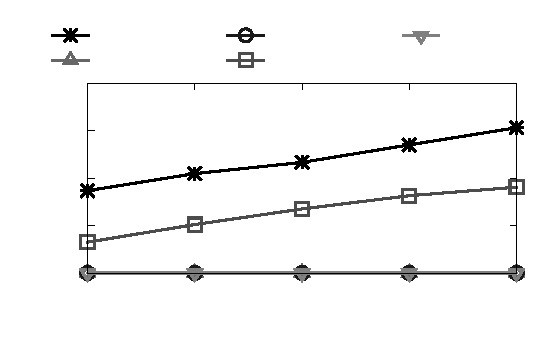
\includegraphics{fig1}}%
    \gplfronttext
  \end{picture}%
\endgroup
}
    \caption{P4 and fat-tree ($\portsPerSwitch=8$)}
    \label{fig:normal_update:p4}
  \end{subfigure}
    \begin{subfigure}[b]{0.49\linewidth}
    \resizebox{\linewidth}{!}{% GNUPLOT: LaTeX picture with Postscript
\begingroup
  \fontfamily{Times-Roman}%
  \selectfont
  \makeatletter
  \providecommand\color[2][]{%
    \GenericError{(gnuplot) \space\space\space\@spaces}{%
      Package color not loaded in conjunction with
      terminal option `colourtext'%
    }{See the gnuplot documentation for explanation.%
    }{Either use 'blacktext' in gnuplot or load the package
      color.sty in LaTeX.}%
    \renewcommand\color[2][]{}%
  }%
  \providecommand\includegraphics[2][]{%
    \GenericError{(gnuplot) \space\space\space\@spaces}{%
      Package graphicx or graphics not loaded%
    }{See the gnuplot documentation for explanation.%
    }{The gnuplot epslatex terminal needs graphicx.sty or graphics.sty.}%
    \renewcommand\includegraphics[2][]{}%
  }%
  \providecommand\rotatebox[2]{#2}%
  \@ifundefined{ifGPcolor}{%
    \newif\ifGPcolor
    \GPcolortrue
  }{}%
  \@ifundefined{ifGPblacktext}{%
    \newif\ifGPblacktext
    \GPblacktexttrue
  }{}%
  % define a \g@addto@macro without @ in the name:
  \let\gplgaddtomacro\g@addto@macro
  % define empty templates for all commands taking text:
  \gdef\gplbacktext{}%
  \gdef\gplfronttext{}%
  \makeatother
  \ifGPblacktext
    % no textcolor at all
    \def\colorrgb#1{}%
    \def\colorgray#1{}%
  \else
    % gray or color?
    \ifGPcolor
      \def\colorrgb#1{\color[rgb]{#1}}%
      \def\colorgray#1{\color[gray]{#1}}%
      \expandafter\def\csname LTw\endcsname{\color{white}}%
      \expandafter\def\csname LTb\endcsname{\color{black}}%
      \expandafter\def\csname LTa\endcsname{\color{black}}%
      \expandafter\def\csname LT0\endcsname{\color[rgb]{1,0,0}}%
      \expandafter\def\csname LT1\endcsname{\color[rgb]{0,1,0}}%
      \expandafter\def\csname LT2\endcsname{\color[rgb]{0,0,1}}%
      \expandafter\def\csname LT3\endcsname{\color[rgb]{1,0,1}}%
      \expandafter\def\csname LT4\endcsname{\color[rgb]{0,1,1}}%
      \expandafter\def\csname LT5\endcsname{\color[rgb]{1,1,0}}%
      \expandafter\def\csname LT6\endcsname{\color[rgb]{0,0,0}}%
      \expandafter\def\csname LT7\endcsname{\color[rgb]{1,0.3,0}}%
      \expandafter\def\csname LT8\endcsname{\color[rgb]{0.5,0.5,0.5}}%
    \else
      % gray
      \def\colorrgb#1{\color{black}}%
      \def\colorgray#1{\color[gray]{#1}}%
      \expandafter\def\csname LTw\endcsname{\color{white}}%
      \expandafter\def\csname LTb\endcsname{\color{black}}%
      \expandafter\def\csname LTa\endcsname{\color{black}}%
      \expandafter\def\csname LT0\endcsname{\color{black}}%
      \expandafter\def\csname LT1\endcsname{\color{black}}%
      \expandafter\def\csname LT2\endcsname{\color{black}}%
      \expandafter\def\csname LT3\endcsname{\color{black}}%
      \expandafter\def\csname LT4\endcsname{\color{black}}%
      \expandafter\def\csname LT5\endcsname{\color{black}}%
      \expandafter\def\csname LT6\endcsname{\color{black}}%
      \expandafter\def\csname LT7\endcsname{\color{black}}%
      \expandafter\def\csname LT8\endcsname{\color{black}}%
    \fi
  \fi
    \setlength{\unitlength}{0.0500bp}%
    \ifx\gptboxheight\undefined%
      \newlength{\gptboxheight}%
      \newlength{\gptboxwidth}%
      \newsavebox{\gptboxtext}%
    \fi%
    \setlength{\fboxrule}{0.5pt}%
    \setlength{\fboxsep}{1pt}%
\begin{picture}(4896.00,3024.00)%
    \gplgaddtomacro\gplbacktext{%
      \csname LTb\endcsname%
      \put(560,560){\makebox(0,0)[r]{\strut{}$0$}}%
      \put(560,1168){\makebox(0,0)[r]{\strut{}$20$}}%
      \put(560,1775){\makebox(0,0)[r]{\strut{}$40$}}%
      \put(560,2383){\makebox(0,0)[r]{\strut{}$60$}}%
      \put(680,360){\makebox(0,0){\strut{}$600$}}%
      \put(1710,360){\makebox(0,0){\strut{}$700$}}%
      \put(2740,360){\makebox(0,0){\strut{}$800$}}%
      \put(3769,360){\makebox(0,0){\strut{}$900$}}%
      \put(4799,360){\makebox(0,0){\strut{}$1000$}}%
    }%
    \gplgaddtomacro\gplfronttext{%
      \csname LTb\endcsname%
      \put(160,1471){\rotatebox{-270}{\makebox(0,0){\strut{}\ylabel}}}%
      \put(2739,140){\makebox(0,0){\strut{}\xlabel}}%
      \csname LTb\endcsname%
      \put(818,2841){\makebox(0,0)[l]{\strut{}\org}}%
      \csname LTb\endcsname%
      \put(818,2601){\makebox(0,0)[l]{\strut{}\sys}}%
      \csname LTb\endcsname%
      \put(2501,2841){\makebox(0,0)[l]{\strut{}\cu}}%
      \csname LTb\endcsname%
      \put(2501,2601){\makebox(0,0)[l]{\strut{}\coconut}}%
      \csname LTb\endcsname%
      \put(4184,2841){\makebox(0,0)[l]{\strut{}\tsu}}%
    }%
    \gplbacktext
    \put(0,0){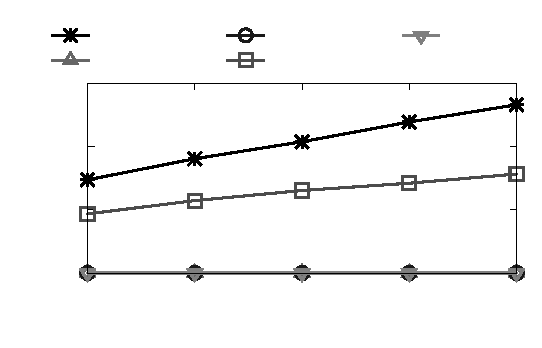
\includegraphics{loss}}%
    \gplfronttext
  \end{picture}%
\endgroup
}
    \caption{OVS and fat-tree ($\portsPerSwitch=8$)}
    \label{fig:normal_update:openvswitch}
  \end{subfigure}
\caption{Packet loss during normal update.  Each data point is an
average of 100 runs.}
\label{fig:normal_update}
\end{figure}

We measured the number of lost packets based on different packet
sending rates when pushing updates to the switches concurrently to
change the paths of packets in the fat-tree topology
($\portsPerSwitch=8$).  As shown in \figref{fig:normal_update}, our
protocol (SCC), TSU, and CU incur no packet loss because these two
mechanisms maintain black-hole freedom.  In addition, we set the TTL
of each packet to be twice its old path length plus its new path
length. So no packet loss also indicates bounded looping, since the
packet will be dropped if its TTL reaches zero.  In contrast, the
normal deployment without any consistent update mechanism and COCONUT
dropped packets because they do not prevent the case where a switch
forwards packets using an old rule to a switch that is not on the new
path for this packet and that has already deleted (or deprecated) its
old rule.  The ``original'' deployment approach also drops packets in
other cases that COCONUT addresses (and that CU, TSU, and SCC also
address).


\subsection{Packet Loss During Link Failure}
\label{sec:eval:link-failure}

\begin{figure}[h]
\centering
  \begin{subfigure}[b]{0.49\linewidth}
    \resizebox{\linewidth}{!}{% GNUPLOT: LaTeX picture with Postscript
\begingroup
  \fontfamily{Times-Roman}%
  \selectfont
  \makeatletter
  \providecommand\color[2][]{%
    \GenericError{(gnuplot) \space\space\space\@spaces}{%
      Package color not loaded in conjunction with
      terminal option `colourtext'%
    }{See the gnuplot documentation for explanation.%
    }{Either use 'blacktext' in gnuplot or load the package
      color.sty in LaTeX.}%
    \renewcommand\color[2][]{}%
  }%
  \providecommand\includegraphics[2][]{%
    \GenericError{(gnuplot) \space\space\space\@spaces}{%
      Package graphicx or graphics not loaded%
    }{See the gnuplot documentation for explanation.%
    }{The gnuplot epslatex terminal needs graphicx.sty or graphics.sty.}%
    \renewcommand\includegraphics[2][]{}%
  }%
  \providecommand\rotatebox[2]{#2}%
  \@ifundefined{ifGPcolor}{%
    \newif\ifGPcolor
    \GPcolortrue
  }{}%
  \@ifundefined{ifGPblacktext}{%
    \newif\ifGPblacktext
    \GPblacktexttrue
  }{}%
  % define a \g@addto@macro without @ in the name:
  \let\gplgaddtomacro\g@addto@macro
  % define empty templates for all commands taking text:
  \gdef\gplbacktext{}%
  \gdef\gplfronttext{}%
  \makeatother
  \ifGPblacktext
    % no textcolor at all
    \def\colorrgb#1{}%
    \def\colorgray#1{}%
  \else
    % gray or color?
    \ifGPcolor
      \def\colorrgb#1{\color[rgb]{#1}}%
      \def\colorgray#1{\color[gray]{#1}}%
      \expandafter\def\csname LTw\endcsname{\color{white}}%
      \expandafter\def\csname LTb\endcsname{\color{black}}%
      \expandafter\def\csname LTa\endcsname{\color{black}}%
      \expandafter\def\csname LT0\endcsname{\color[rgb]{1,0,0}}%
      \expandafter\def\csname LT1\endcsname{\color[rgb]{0,1,0}}%
      \expandafter\def\csname LT2\endcsname{\color[rgb]{0,0,1}}%
      \expandafter\def\csname LT3\endcsname{\color[rgb]{1,0,1}}%
      \expandafter\def\csname LT4\endcsname{\color[rgb]{0,1,1}}%
      \expandafter\def\csname LT5\endcsname{\color[rgb]{1,1,0}}%
      \expandafter\def\csname LT6\endcsname{\color[rgb]{0,0,0}}%
      \expandafter\def\csname LT7\endcsname{\color[rgb]{1,0.3,0}}%
      \expandafter\def\csname LT8\endcsname{\color[rgb]{0.5,0.5,0.5}}%
    \else
      % gray
      \def\colorrgb#1{\color{black}}%
      \def\colorgray#1{\color[gray]{#1}}%
      \expandafter\def\csname LTw\endcsname{\color{white}}%
      \expandafter\def\csname LTb\endcsname{\color{black}}%
      \expandafter\def\csname LTa\endcsname{\color{black}}%
      \expandafter\def\csname LT0\endcsname{\color{black}}%
      \expandafter\def\csname LT1\endcsname{\color{black}}%
      \expandafter\def\csname LT2\endcsname{\color{black}}%
      \expandafter\def\csname LT3\endcsname{\color{black}}%
      \expandafter\def\csname LT4\endcsname{\color{black}}%
      \expandafter\def\csname LT5\endcsname{\color{black}}%
      \expandafter\def\csname LT6\endcsname{\color{black}}%
      \expandafter\def\csname LT7\endcsname{\color{black}}%
      \expandafter\def\csname LT8\endcsname{\color{black}}%
    \fi
  \fi
    \setlength{\unitlength}{0.0500bp}%
    \ifx\gptboxheight\undefined%
      \newlength{\gptboxheight}%
      \newlength{\gptboxwidth}%
      \newsavebox{\gptboxtext}%
    \fi%
    \setlength{\fboxrule}{0.5pt}%
    \setlength{\fboxsep}{1pt}%
\begin{picture}(4896.00,3024.00)%
    \gplgaddtomacro\gplbacktext{%
      \csname LTb\endcsname%
      \put(680,560){\makebox(0,0)[r]{\strut{}$0$}}%
      \put(680,925){\makebox(0,0)[r]{\strut{}$100$}}%
      \put(680,1289){\makebox(0,0)[r]{\strut{}$200$}}%
      \put(680,1654){\makebox(0,0)[r]{\strut{}$300$}}%
      \put(680,2018){\makebox(0,0)[r]{\strut{}$400$}}%
      \put(680,2383){\makebox(0,0)[r]{\strut{}$500$}}%
      \put(800,360){\makebox(0,0){\strut{}$600$}}%
      \put(1800,360){\makebox(0,0){\strut{}$700$}}%
      \put(2800,360){\makebox(0,0){\strut{}$800$}}%
      \put(3799,360){\makebox(0,0){\strut{}$900$}}%
      \put(4799,360){\makebox(0,0){\strut{}$1000$}}%
    }%
    \gplgaddtomacro\gplfronttext{%
      \csname LTb\endcsname%
      \put(160,1471){\rotatebox{-270}{\makebox(0,0){\strut{}\ylabel}}}%
      \put(2799,140){\makebox(0,0){\strut{}\xlabel}}%
      \csname LTb\endcsname%
      \put(878,2841){\makebox(0,0)[l]{\strut{}\org}}%
      \csname LTb\endcsname%
      \put(878,2601){\makebox(0,0)[l]{\strut{}\sys}}%
      \csname LTb\endcsname%
      \put(2561,2841){\makebox(0,0)[l]{\strut{}\cu}}%
      \csname LTb\endcsname%
      \put(2561,2601){\makebox(0,0)[l]{\strut{}\coconut}}%
      \csname LTb\endcsname%
      \put(4244,2841){\makebox(0,0)[l]{\strut{}\tsu}}%
    }%
    \gplbacktext
    \put(0,0){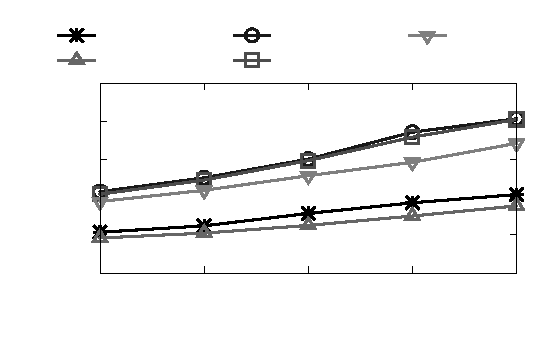
\includegraphics{fig2}}%
    \gplfronttext
  \end{picture}%
\endgroup
}
    \caption{P4 and fat-tree ($\portsPerSwitch=8$)}
    \label{fig:link_failure:fat_tree-p4}
  \end{subfigure}
    \begin{subfigure}[b]{0.49\linewidth}
    \resizebox{\linewidth}{!}{% GNUPLOT: LaTeX picture with Postscript
\begingroup
  \fontfamily{Times-Roman}%
  \selectfont
  \makeatletter
  \providecommand\color[2][]{%
    \GenericError{(gnuplot) \space\space\space\@spaces}{%
      Package color not loaded in conjunction with
      terminal option `colourtext'%
    }{See the gnuplot documentation for explanation.%
    }{Either use 'blacktext' in gnuplot or load the package
      color.sty in LaTeX.}%
    \renewcommand\color[2][]{}%
  }%
  \providecommand\includegraphics[2][]{%
    \GenericError{(gnuplot) \space\space\space\@spaces}{%
      Package graphicx or graphics not loaded%
    }{See the gnuplot documentation for explanation.%
    }{The gnuplot epslatex terminal needs graphicx.sty or graphics.sty.}%
    \renewcommand\includegraphics[2][]{}%
  }%
  \providecommand\rotatebox[2]{#2}%
  \@ifundefined{ifGPcolor}{%
    \newif\ifGPcolor
    \GPcolortrue
  }{}%
  \@ifundefined{ifGPblacktext}{%
    \newif\ifGPblacktext
    \GPblacktexttrue
  }{}%
  % define a \g@addto@macro without @ in the name:
  \let\gplgaddtomacro\g@addto@macro
  % define empty templates for all commands taking text:
  \gdef\gplbacktext{}%
  \gdef\gplfronttext{}%
  \makeatother
  \ifGPblacktext
    % no textcolor at all
    \def\colorrgb#1{}%
    \def\colorgray#1{}%
  \else
    % gray or color?
    \ifGPcolor
      \def\colorrgb#1{\color[rgb]{#1}}%
      \def\colorgray#1{\color[gray]{#1}}%
      \expandafter\def\csname LTw\endcsname{\color{white}}%
      \expandafter\def\csname LTb\endcsname{\color{black}}%
      \expandafter\def\csname LTa\endcsname{\color{black}}%
      \expandafter\def\csname LT0\endcsname{\color[rgb]{1,0,0}}%
      \expandafter\def\csname LT1\endcsname{\color[rgb]{0,1,0}}%
      \expandafter\def\csname LT2\endcsname{\color[rgb]{0,0,1}}%
      \expandafter\def\csname LT3\endcsname{\color[rgb]{1,0,1}}%
      \expandafter\def\csname LT4\endcsname{\color[rgb]{0,1,1}}%
      \expandafter\def\csname LT5\endcsname{\color[rgb]{1,1,0}}%
      \expandafter\def\csname LT6\endcsname{\color[rgb]{0,0,0}}%
      \expandafter\def\csname LT7\endcsname{\color[rgb]{1,0.3,0}}%
      \expandafter\def\csname LT8\endcsname{\color[rgb]{0.5,0.5,0.5}}%
    \else
      % gray
      \def\colorrgb#1{\color{black}}%
      \def\colorgray#1{\color[gray]{#1}}%
      \expandafter\def\csname LTw\endcsname{\color{white}}%
      \expandafter\def\csname LTb\endcsname{\color{black}}%
      \expandafter\def\csname LTa\endcsname{\color{black}}%
      \expandafter\def\csname LT0\endcsname{\color{black}}%
      \expandafter\def\csname LT1\endcsname{\color{black}}%
      \expandafter\def\csname LT2\endcsname{\color{black}}%
      \expandafter\def\csname LT3\endcsname{\color{black}}%
      \expandafter\def\csname LT4\endcsname{\color{black}}%
      \expandafter\def\csname LT5\endcsname{\color{black}}%
      \expandafter\def\csname LT6\endcsname{\color{black}}%
      \expandafter\def\csname LT7\endcsname{\color{black}}%
      \expandafter\def\csname LT8\endcsname{\color{black}}%
    \fi
  \fi
    \setlength{\unitlength}{0.0500bp}%
    \ifx\gptboxheight\undefined%
      \newlength{\gptboxheight}%
      \newlength{\gptboxwidth}%
      \newsavebox{\gptboxtext}%
    \fi%
    \setlength{\fboxrule}{0.5pt}%
    \setlength{\fboxsep}{1pt}%
\begin{picture}(4896.00,3024.00)%
    \gplgaddtomacro\gplbacktext{%
      \csname LTb\endcsname%
      \put(680,560){\makebox(0,0)[r]{\strut{}$0$}}%
      \put(680,1016){\makebox(0,0)[r]{\strut{}$100$}}%
      \put(680,1472){\makebox(0,0)[r]{\strut{}$200$}}%
      \put(680,1927){\makebox(0,0)[r]{\strut{}$300$}}%
      \put(680,2383){\makebox(0,0)[r]{\strut{}$400$}}%
      \put(800,360){\makebox(0,0){\strut{}$600$}}%
      \put(1800,360){\makebox(0,0){\strut{}$700$}}%
      \put(2800,360){\makebox(0,0){\strut{}$800$}}%
      \put(3799,360){\makebox(0,0){\strut{}$900$}}%
      \put(4799,360){\makebox(0,0){\strut{}$1000$}}%
    }%
    \gplgaddtomacro\gplfronttext{%
      \csname LTb\endcsname%
      \put(160,1471){\rotatebox{-270}{\makebox(0,0){\strut{}\ylabel}}}%
      \put(2799,140){\makebox(0,0){\strut{}\xlabel}}%
      \csname LTb\endcsname%
      \put(878,2841){\makebox(0,0)[l]{\strut{}\org}}%
      \csname LTb\endcsname%
      \put(878,2601){\makebox(0,0)[l]{\strut{}\sys}}%
      \csname LTb\endcsname%
      \put(2561,2841){\makebox(0,0)[l]{\strut{}\cu}}%
      \csname LTb\endcsname%
      \put(2561,2601){\makebox(0,0)[l]{\strut{}\coconut}}%
      \csname LTb\endcsname%
      \put(4244,2841){\makebox(0,0)[l]{\strut{}\tsu}}%
    }%
    \gplbacktext
    \put(0,0){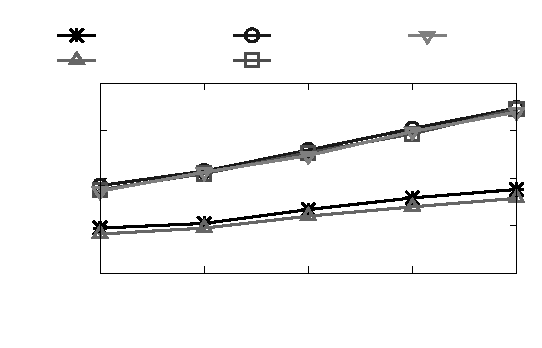
\includegraphics{loss2}}%
    \gplfronttext
  \end{picture}%
\endgroup
}
    \caption{OVS and fat-tree ($\portsPerSwitch=8$)}
    \label{fig:link_failure:fat_tree-ovs}
  \end{subfigure}
    \begin{subfigure}[b]{0.49\linewidth}
    \resizebox{\linewidth}{!}{% GNUPLOT: LaTeX picture with Postscript
\begingroup
  \fontfamily{Times-Roman}%
  \selectfont
  \makeatletter
  \providecommand\color[2][]{%
    \GenericError{(gnuplot) \space\space\space\@spaces}{%
      Package color not loaded in conjunction with
      terminal option `colourtext'%
    }{See the gnuplot documentation for explanation.%
    }{Either use 'blacktext' in gnuplot or load the package
      color.sty in LaTeX.}%
    \renewcommand\color[2][]{}%
  }%
  \providecommand\includegraphics[2][]{%
    \GenericError{(gnuplot) \space\space\space\@spaces}{%
      Package graphicx or graphics not loaded%
    }{See the gnuplot documentation for explanation.%
    }{The gnuplot epslatex terminal needs graphicx.sty or graphics.sty.}%
    \renewcommand\includegraphics[2][]{}%
  }%
  \providecommand\rotatebox[2]{#2}%
  \@ifundefined{ifGPcolor}{%
    \newif\ifGPcolor
    \GPcolortrue
  }{}%
  \@ifundefined{ifGPblacktext}{%
    \newif\ifGPblacktext
    \GPblacktexttrue
  }{}%
  % define a \g@addto@macro without @ in the name:
  \let\gplgaddtomacro\g@addto@macro
  % define empty templates for all commands taking text:
  \gdef\gplbacktext{}%
  \gdef\gplfronttext{}%
  \makeatother
  \ifGPblacktext
    % no textcolor at all
    \def\colorrgb#1{}%
    \def\colorgray#1{}%
  \else
    % gray or color?
    \ifGPcolor
      \def\colorrgb#1{\color[rgb]{#1}}%
      \def\colorgray#1{\color[gray]{#1}}%
      \expandafter\def\csname LTw\endcsname{\color{white}}%
      \expandafter\def\csname LTb\endcsname{\color{black}}%
      \expandafter\def\csname LTa\endcsname{\color{black}}%
      \expandafter\def\csname LT0\endcsname{\color[rgb]{1,0,0}}%
      \expandafter\def\csname LT1\endcsname{\color[rgb]{0,1,0}}%
      \expandafter\def\csname LT2\endcsname{\color[rgb]{0,0,1}}%
      \expandafter\def\csname LT3\endcsname{\color[rgb]{1,0,1}}%
      \expandafter\def\csname LT4\endcsname{\color[rgb]{0,1,1}}%
      \expandafter\def\csname LT5\endcsname{\color[rgb]{1,1,0}}%
      \expandafter\def\csname LT6\endcsname{\color[rgb]{0,0,0}}%
      \expandafter\def\csname LT7\endcsname{\color[rgb]{1,0.3,0}}%
      \expandafter\def\csname LT8\endcsname{\color[rgb]{0.5,0.5,0.5}}%
    \else
      % gray
      \def\colorrgb#1{\color{black}}%
      \def\colorgray#1{\color[gray]{#1}}%
      \expandafter\def\csname LTw\endcsname{\color{white}}%
      \expandafter\def\csname LTb\endcsname{\color{black}}%
      \expandafter\def\csname LTa\endcsname{\color{black}}%
      \expandafter\def\csname LT0\endcsname{\color{black}}%
      \expandafter\def\csname LT1\endcsname{\color{black}}%
      \expandafter\def\csname LT2\endcsname{\color{black}}%
      \expandafter\def\csname LT3\endcsname{\color{black}}%
      \expandafter\def\csname LT4\endcsname{\color{black}}%
      \expandafter\def\csname LT5\endcsname{\color{black}}%
      \expandafter\def\csname LT6\endcsname{\color{black}}%
      \expandafter\def\csname LT7\endcsname{\color{black}}%
      \expandafter\def\csname LT8\endcsname{\color{black}}%
    \fi
  \fi
    \setlength{\unitlength}{0.0500bp}%
    \ifx\gptboxheight\undefined%
      \newlength{\gptboxheight}%
      \newlength{\gptboxwidth}%
      \newsavebox{\gptboxtext}%
    \fi%
    \setlength{\fboxrule}{0.5pt}%
    \setlength{\fboxsep}{1pt}%
\begin{picture}(4896.00,3024.00)%
    \gplgaddtomacro\gplbacktext{%
      \csname LTb\endcsname%
      \put(680,560){\makebox(0,0)[r]{\strut{}$0$}}%
      \put(680,925){\makebox(0,0)[r]{\strut{}$100$}}%
      \put(680,1289){\makebox(0,0)[r]{\strut{}$200$}}%
      \put(680,1654){\makebox(0,0)[r]{\strut{}$300$}}%
      \put(680,2018){\makebox(0,0)[r]{\strut{}$400$}}%
      \put(680,2383){\makebox(0,0)[r]{\strut{}$500$}}%
      \put(800,360){\makebox(0,0){\strut{}$600$}}%
      \put(1800,360){\makebox(0,0){\strut{}$700$}}%
      \put(2800,360){\makebox(0,0){\strut{}$800$}}%
      \put(3799,360){\makebox(0,0){\strut{}$900$}}%
      \put(4799,360){\makebox(0,0){\strut{}$1000$}}%
    }%
    \gplgaddtomacro\gplfronttext{%
      \csname LTb\endcsname%
      \put(160,1471){\rotatebox{-270}{\makebox(0,0){\strut{}\ylabel}}}%
      \put(2799,140){\makebox(0,0){\strut{}\xlabel}}%
      \csname LTb\endcsname%
      \put(878,2841){\makebox(0,0)[l]{\strut{}\org}}%
      \csname LTb\endcsname%
      \put(878,2601){\makebox(0,0)[l]{\strut{}\sys}}%
      \csname LTb\endcsname%
      \put(2561,2841){\makebox(0,0)[l]{\strut{}\cu}}%
      \csname LTb\endcsname%
      \put(2561,2601){\makebox(0,0)[l]{\strut{}\coconut}}%
      \csname LTb\endcsname%
      \put(4244,2841){\makebox(0,0)[l]{\strut{}\tsu}}%
    }%
    \gplbacktext
    \put(0,0){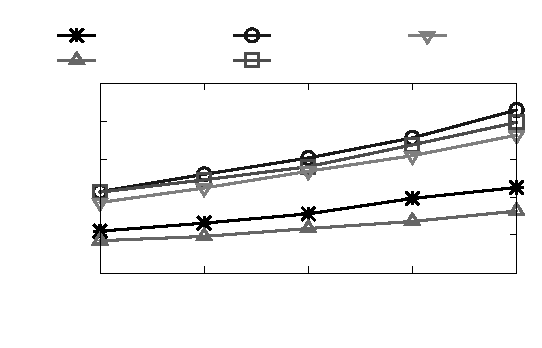
\includegraphics{fig5}}%
    \gplfronttext
  \end{picture}%
\endgroup
}
    \caption{P4 and DFN topology}
    \label{fig:link_failure:dfn}
  \end{subfigure}
  \caption{Packet loss during link failure.  Each data point is an
  average of 100 runs.}
  \label{fig:link_failure}
\end{figure}

In the tests reported in this section, we broke one randomly chosen
link of some existing path, forcing a new epoch with new paths for
the flows traversing that link.  During the delay to update the network with the new
paths, packets on those flows were lost.  For the $\portsPerSwitch=8$
fat-tree topology
(\figrefs{fig:link_failure:fat_tree-p4}{fig:link_failure:fat_tree-ovs}),
the response time included rule generation (i.e., the delay for
executing our algorithm), while we pre-computed the rules for the DFN
topology (\figref{fig:link_failure:dfn}).  The DFN results for Open
vSwitch are similar to those for P4 and so are omitted for brevity.
As we can see in \figref{fig:link_failure}, SCC dropped fewer packets
than COCONUT, TSU, and CU because our protocol has smaller delay to
put the new configuration in place. Specifically, in SCC, new rules
can be applied as soon as they are installed in the switch.  However,
CU and COCONUT require that updated rules reach all switches on the
new paths before any of them can start to be used to route packets, and
TSU deploys new rules over multiple steps. Also, SCC outperforms the
``original'' deployment due to the consistency that SCC offers; e.g.,
SCC prevents packets forwarded using a new rule from then being
matched to an old rule or otherwise dropped.

\subsection{Rule Deployment Time}
\label{sec:eval:deployment}

In the tests reported in this section, we measured the deployment time
of rule updates, including both the new rule installation and old rule
cleanup (and, in our case, send-back rule cleanup).  Each epoch in
these tests involved one path change, and \figref{fig:completion_time}
shows the distribution of rule deployment times for 100 such epochs
for the fat-tree topology ($\portsPerSwitch=8$).  SCC rule deployment
is considerably faster than TSU, CU and COCONUT, with the vast
majority of the 100 SCC deployments completing before even a minority
of the TSU and CU deployments and well before any COCONUT deployments.
Total completion time of SCC is only slightly larger than for the
``original'' protocol, owing to extra rule cleanup.

\begin{figure}[h]
\centering
  \begin{subfigure}[b]{0.49\linewidth}
    \resizebox{\linewidth}{!}{% GNUPLOT: LaTeX picture with Postscript
\begingroup
  \fontfamily{Times-Roman}%
  \selectfont
  \makeatletter
  \providecommand\color[2][]{%
    \GenericError{(gnuplot) \space\space\space\@spaces}{%
      Package color not loaded in conjunction with
      terminal option `colourtext'%
    }{See the gnuplot documentation for explanation.%
    }{Either use 'blacktext' in gnuplot or load the package
      color.sty in LaTeX.}%
    \renewcommand\color[2][]{}%
  }%
  \providecommand\includegraphics[2][]{%
    \GenericError{(gnuplot) \space\space\space\@spaces}{%
      Package graphicx or graphics not loaded%
    }{See the gnuplot documentation for explanation.%
    }{The gnuplot epslatex terminal needs graphicx.sty or graphics.sty.}%
    \renewcommand\includegraphics[2][]{}%
  }%
  \providecommand\rotatebox[2]{#2}%
  \@ifundefined{ifGPcolor}{%
    \newif\ifGPcolor
    \GPcolortrue
  }{}%
  \@ifundefined{ifGPblacktext}{%
    \newif\ifGPblacktext
    \GPblacktexttrue
  }{}%
  % define a \g@addto@macro without @ in the name:
  \let\gplgaddtomacro\g@addto@macro
  % define empty templates for all commands taking text:
  \gdef\gplbacktext{}%
  \gdef\gplfronttext{}%
  \makeatother
  \ifGPblacktext
    % no textcolor at all
    \def\colorrgb#1{}%
    \def\colorgray#1{}%
  \else
    % gray or color?
    \ifGPcolor
      \def\colorrgb#1{\color[rgb]{#1}}%
      \def\colorgray#1{\color[gray]{#1}}%
      \expandafter\def\csname LTw\endcsname{\color{white}}%
      \expandafter\def\csname LTb\endcsname{\color{black}}%
      \expandafter\def\csname LTa\endcsname{\color{black}}%
      \expandafter\def\csname LT0\endcsname{\color[rgb]{1,0,0}}%
      \expandafter\def\csname LT1\endcsname{\color[rgb]{0,1,0}}%
      \expandafter\def\csname LT2\endcsname{\color[rgb]{0,0,1}}%
      \expandafter\def\csname LT3\endcsname{\color[rgb]{1,0,1}}%
      \expandafter\def\csname LT4\endcsname{\color[rgb]{0,1,1}}%
      \expandafter\def\csname LT5\endcsname{\color[rgb]{1,1,0}}%
      \expandafter\def\csname LT6\endcsname{\color[rgb]{0,0,0}}%
      \expandafter\def\csname LT7\endcsname{\color[rgb]{1,0.3,0}}%
      \expandafter\def\csname LT8\endcsname{\color[rgb]{0.5,0.5,0.5}}%
    \else
      % gray
      \def\colorrgb#1{\color{black}}%
      \def\colorgray#1{\color[gray]{#1}}%
      \expandafter\def\csname LTw\endcsname{\color{white}}%
      \expandafter\def\csname LTb\endcsname{\color{black}}%
      \expandafter\def\csname LTa\endcsname{\color{black}}%
      \expandafter\def\csname LT0\endcsname{\color{black}}%
      \expandafter\def\csname LT1\endcsname{\color{black}}%
      \expandafter\def\csname LT2\endcsname{\color{black}}%
      \expandafter\def\csname LT3\endcsname{\color{black}}%
      \expandafter\def\csname LT4\endcsname{\color{black}}%
      \expandafter\def\csname LT5\endcsname{\color{black}}%
      \expandafter\def\csname LT6\endcsname{\color{black}}%
      \expandafter\def\csname LT7\endcsname{\color{black}}%
      \expandafter\def\csname LT8\endcsname{\color{black}}%
    \fi
  \fi
    \setlength{\unitlength}{0.0500bp}%
    \ifx\gptboxheight\undefined%
      \newlength{\gptboxheight}%
      \newlength{\gptboxwidth}%
      \newsavebox{\gptboxtext}%
    \fi%
    \setlength{\fboxrule}{0.5pt}%
    \setlength{\fboxsep}{1pt}%
\begin{picture}(4896.00,3024.00)%
    \gplgaddtomacro\gplbacktext{%
      \csname LTb\endcsname%
      \put(540,975){\makebox(0,0)[r]{\strut{}$0.2$}}%
      \csname LTb\endcsname%
      \put(540,1327){\makebox(0,0)[r]{\strut{}$0.4$}}%
      \csname LTb\endcsname%
      \put(540,1679){\makebox(0,0)[r]{\strut{}$0.6$}}%
      \csname LTb\endcsname%
      \put(540,2031){\makebox(0,0)[r]{\strut{}$0.8$}}%
      \csname LTb\endcsname%
      \put(540,2383){\makebox(0,0)[r]{\strut{}$1$}}%
      \csname LTb\endcsname%
      \put(660,440){\makebox(0,0){\strut{}$0$}}%
      \csname LTb\endcsname%
      \put(1036,440){\makebox(0,0){\strut{}$0.1$}}%
      \csname LTb\endcsname%
      \put(1413,440){\makebox(0,0){\strut{}$0.2$}}%
      \csname LTb\endcsname%
      \put(1789,440){\makebox(0,0){\strut{}$0.3$}}%
      \csname LTb\endcsname%
      \put(2165,440){\makebox(0,0){\strut{}$0.4$}}%
      \csname LTb\endcsname%
      \put(2541,440){\makebox(0,0){\strut{}$0.5$}}%
      \csname LTb\endcsname%
      \put(2918,440){\makebox(0,0){\strut{}$0.6$}}%
      \csname LTb\endcsname%
      \put(3294,440){\makebox(0,0){\strut{}$0.7$}}%
      \csname LTb\endcsname%
      \put(3670,440){\makebox(0,0){\strut{}$0.8$}}%
      \csname LTb\endcsname%
      \put(4046,440){\makebox(0,0){\strut{}$0.9$}}%
      \csname LTb\endcsname%
      \put(4423,440){\makebox(0,0){\strut{}$1$}}%
      \csname LTb\endcsname%
      \put(4799,440){\makebox(0,0){\strut{}$1.1$}}%
    }%
    \gplgaddtomacro\gplfronttext{%
      \csname LTb\endcsname%
      \put(200,1511){\rotatebox{-270}{\makebox(0,0){\strut{}}}}%
      \put(2729,140){\makebox(0,0){\strut{}\updateTime(s)}}%
      \csname LTb\endcsname%
      \put(808,2841){\makebox(0,0)[l]{\strut{}\org}}%
      \csname LTb\endcsname%
      \put(808,2601){\makebox(0,0)[l]{\strut{}\sys}}%
      \csname LTb\endcsname%
      \put(2491,2841){\makebox(0,0)[l]{\strut{}\cu}}%
      \csname LTb\endcsname%
      \put(2491,2601){\makebox(0,0)[l]{\strut{}\coconut}}%
      \csname LTb\endcsname%
      \put(4174,2841){\makebox(0,0)[l]{\strut{}\tsu}}%
    }%
    \gplbacktext
    \put(0,0){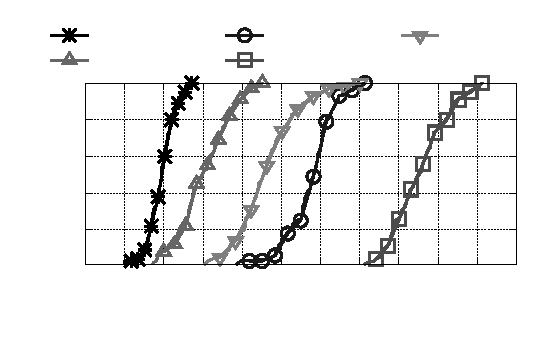
\includegraphics{p4CDF}}%
    \gplfronttext
  \end{picture}%
\endgroup
}
    \caption{P4 and fat-tree ($\portsPerSwitch=8$)}
    \label{fig:completion_time:p4}
  \end{subfigure}
    \begin{subfigure}[b]{0.49\linewidth}
    \resizebox{\linewidth}{!}{% GNUPLOT: LaTeX picture with Postscript
\begingroup
  \fontfamily{Times-Roman}%
  \selectfont
  \makeatletter
  \providecommand\color[2][]{%
    \GenericError{(gnuplot) \space\space\space\@spaces}{%
      Package color not loaded in conjunction with
      terminal option `colourtext'%
    }{See the gnuplot documentation for explanation.%
    }{Either use 'blacktext' in gnuplot or load the package
      color.sty in LaTeX.}%
    \renewcommand\color[2][]{}%
  }%
  \providecommand\includegraphics[2][]{%
    \GenericError{(gnuplot) \space\space\space\@spaces}{%
      Package graphicx or graphics not loaded%
    }{See the gnuplot documentation for explanation.%
    }{The gnuplot epslatex terminal needs graphicx.sty or graphics.sty.}%
    \renewcommand\includegraphics[2][]{}%
  }%
  \providecommand\rotatebox[2]{#2}%
  \@ifundefined{ifGPcolor}{%
    \newif\ifGPcolor
    \GPcolortrue
  }{}%
  \@ifundefined{ifGPblacktext}{%
    \newif\ifGPblacktext
    \GPblacktexttrue
  }{}%
  % define a \g@addto@macro without @ in the name:
  \let\gplgaddtomacro\g@addto@macro
  % define empty templates for all commands taking text:
  \gdef\gplbacktext{}%
  \gdef\gplfronttext{}%
  \makeatother
  \ifGPblacktext
    % no textcolor at all
    \def\colorrgb#1{}%
    \def\colorgray#1{}%
  \else
    % gray or color?
    \ifGPcolor
      \def\colorrgb#1{\color[rgb]{#1}}%
      \def\colorgray#1{\color[gray]{#1}}%
      \expandafter\def\csname LTw\endcsname{\color{white}}%
      \expandafter\def\csname LTb\endcsname{\color{black}}%
      \expandafter\def\csname LTa\endcsname{\color{black}}%
      \expandafter\def\csname LT0\endcsname{\color[rgb]{1,0,0}}%
      \expandafter\def\csname LT1\endcsname{\color[rgb]{0,1,0}}%
      \expandafter\def\csname LT2\endcsname{\color[rgb]{0,0,1}}%
      \expandafter\def\csname LT3\endcsname{\color[rgb]{1,0,1}}%
      \expandafter\def\csname LT4\endcsname{\color[rgb]{0,1,1}}%
      \expandafter\def\csname LT5\endcsname{\color[rgb]{1,1,0}}%
      \expandafter\def\csname LT6\endcsname{\color[rgb]{0,0,0}}%
      \expandafter\def\csname LT7\endcsname{\color[rgb]{1,0.3,0}}%
      \expandafter\def\csname LT8\endcsname{\color[rgb]{0.5,0.5,0.5}}%
    \else
      % gray
      \def\colorrgb#1{\color{black}}%
      \def\colorgray#1{\color[gray]{#1}}%
      \expandafter\def\csname LTw\endcsname{\color{white}}%
      \expandafter\def\csname LTb\endcsname{\color{black}}%
      \expandafter\def\csname LTa\endcsname{\color{black}}%
      \expandafter\def\csname LT0\endcsname{\color{black}}%
      \expandafter\def\csname LT1\endcsname{\color{black}}%
      \expandafter\def\csname LT2\endcsname{\color{black}}%
      \expandafter\def\csname LT3\endcsname{\color{black}}%
      \expandafter\def\csname LT4\endcsname{\color{black}}%
      \expandafter\def\csname LT5\endcsname{\color{black}}%
      \expandafter\def\csname LT6\endcsname{\color{black}}%
      \expandafter\def\csname LT7\endcsname{\color{black}}%
      \expandafter\def\csname LT8\endcsname{\color{black}}%
    \fi
  \fi
    \setlength{\unitlength}{0.0500bp}%
    \ifx\gptboxheight\undefined%
      \newlength{\gptboxheight}%
      \newlength{\gptboxwidth}%
      \newsavebox{\gptboxtext}%
    \fi%
    \setlength{\fboxrule}{0.5pt}%
    \setlength{\fboxsep}{1pt}%
\begin{picture}(4896.00,3024.00)%
    \gplgaddtomacro\gplbacktext{%
      \csname LTb\endcsname%
      \put(540,975){\makebox(0,0)[r]{\strut{}$0.2$}}%
      \csname LTb\endcsname%
      \put(540,1327){\makebox(0,0)[r]{\strut{}$0.4$}}%
      \csname LTb\endcsname%
      \put(540,1679){\makebox(0,0)[r]{\strut{}$0.6$}}%
      \csname LTb\endcsname%
      \put(540,2031){\makebox(0,0)[r]{\strut{}$0.8$}}%
      \csname LTb\endcsname%
      \put(540,2383){\makebox(0,0)[r]{\strut{}$1$}}%
      \csname LTb\endcsname%
      \put(660,440){\makebox(0,0){\strut{}$0.1$}}%
      \csname LTb\endcsname%
      \put(1074,440){\makebox(0,0){\strut{}$0.2$}}%
      \csname LTb\endcsname%
      \put(1488,440){\makebox(0,0){\strut{}$0.3$}}%
      \csname LTb\endcsname%
      \put(1902,440){\makebox(0,0){\strut{}$0.4$}}%
      \csname LTb\endcsname%
      \put(2316,440){\makebox(0,0){\strut{}$0.5$}}%
      \csname LTb\endcsname%
      \put(2730,440){\makebox(0,0){\strut{}$0.6$}}%
      \csname LTb\endcsname%
      \put(3143,440){\makebox(0,0){\strut{}$0.7$}}%
      \csname LTb\endcsname%
      \put(3557,440){\makebox(0,0){\strut{}$0.8$}}%
      \csname LTb\endcsname%
      \put(3971,440){\makebox(0,0){\strut{}$0.9$}}%
      \csname LTb\endcsname%
      \put(4385,440){\makebox(0,0){\strut{}$1$}}%
      \csname LTb\endcsname%
      \put(4799,440){\makebox(0,0){\strut{}$1.1$}}%
    }%
    \gplgaddtomacro\gplfronttext{%
      \csname LTb\endcsname%
      \put(200,1511){\rotatebox{-270}{\makebox(0,0){\strut{}}}}%
      \put(2729,140){\makebox(0,0){\strut{}\updateTime(s)}}%
      \csname LTb\endcsname%
      \put(808,2841){\makebox(0,0)[l]{\strut{}\org}}%
      \csname LTb\endcsname%
      \put(808,2601){\makebox(0,0)[l]{\strut{}\sys}}%
      \csname LTb\endcsname%
      \put(2491,2841){\makebox(0,0)[l]{\strut{}\cu}}%
      \csname LTb\endcsname%
      \put(2491,2601){\makebox(0,0)[l]{\strut{}\coconut}}%
      \csname LTb\endcsname%
      \put(4174,2841){\makebox(0,0)[l]{\strut{}\tsu}}%
    }%
    \gplbacktext
    \put(0,0){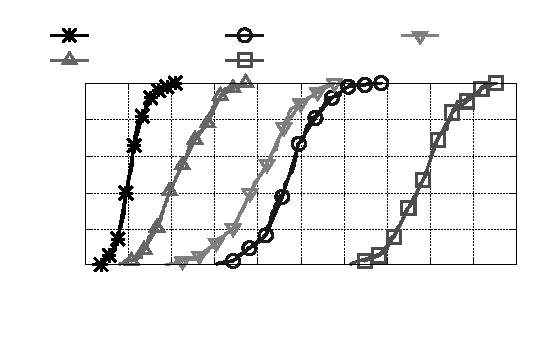
\includegraphics{dfnCDF}}%
    \gplfronttext
  \end{picture}%
\endgroup
}
    \caption{P4 and DFN}
    \label{fig:completion_time:openvswitch}
  \end{subfigure}
\caption{CDF of rule deployment times over 100 epochs.}
\label{fig:completion_time}
\end{figure}

SCC outperforms CU and COCONUT during rule deployment for two reasons.
First, SCC simply deploys rules to fewer switches, since it attempts
to minimize the number of switches to which it must do so.  Second,
SCC involves fewer phases of communication between the controller and
switches.  Here, COCONUT is worse than CU because it requires more
time to clean up old rules.  TSU is better than CU because CU needs to
update more switches.

\subsection{Memory Overhead in Switches}
\label{sec:eval:rules}

To evaluate the number of rules imposed on the switches by each
algorithm, we examined the per-switch logs of rule installations and
deletions over 100 consecutive path changes in the fat-tree topology
($\portsPerSwitch=8$).  We computed a time series of the total number
of rules installed across all switches in the network, if all 100 path
changes were included in one epoch.  This time series for each of SCC,
CU, and COCONUT is shown in \figref{fig:rule_number:fat_tree}.  We
repeated this evaluation on the DFN topology, but by breaking the
``busiest'' link; see \figref{fig:rule_number:dfn}.  Here, the
``busiest'' link is the link that causes the most path changes when
the link fails, which was 306 path changes in this case.  As these
figures show, SCC induced a rule overhead of significantly fewer rules
than CU and COCONUT, because SCC installs extra, send-back rules only
on selected switches on old paths.  In particular, SCC does not
temporarily retain old rules along with new rules, like CU and COCONUT
do.  Though TSU does not add extra rules on switches, old rules are
kept longer because TSU executes in multiple steps.


\begin{figure}[h]
\centering
  \begin{subfigure}[b]{0.49\linewidth}
    \resizebox{\linewidth}{!}{\footnotesize% GNUPLOT: LaTeX picture with Postscript
\begingroup
  \fontfamily{Times-Roman}%
  \selectfont
  \makeatletter
  \providecommand\color[2][]{%
    \GenericError{(gnuplot) \space\space\space\@spaces}{%
      Package color not loaded in conjunction with
      terminal option `colourtext'%
    }{See the gnuplot documentation for explanation.%
    }{Either use 'blacktext' in gnuplot or load the package
      color.sty in LaTeX.}%
    \renewcommand\color[2][]{}%
  }%
  \providecommand\includegraphics[2][]{%
    \GenericError{(gnuplot) \space\space\space\@spaces}{%
      Package graphicx or graphics not loaded%
    }{See the gnuplot documentation for explanation.%
    }{The gnuplot epslatex terminal needs graphicx.sty or graphics.sty.}%
    \renewcommand\includegraphics[2][]{}%
  }%
  \providecommand\rotatebox[2]{#2}%
  \@ifundefined{ifGPcolor}{%
    \newif\ifGPcolor
    \GPcolortrue
  }{}%
  \@ifundefined{ifGPblacktext}{%
    \newif\ifGPblacktext
    \GPblacktexttrue
  }{}%
  % define a \g@addto@macro without @ in the name:
  \let\gplgaddtomacro\g@addto@macro
  % define empty templates for all commands taking text:
  \gdef\gplbacktext{}%
  \gdef\gplfronttext{}%
  \makeatother
  \ifGPblacktext
    % no textcolor at all
    \def\colorrgb#1{}%
    \def\colorgray#1{}%
  \else
    % gray or color?
    \ifGPcolor
      \def\colorrgb#1{\color[rgb]{#1}}%
      \def\colorgray#1{\color[gray]{#1}}%
      \expandafter\def\csname LTw\endcsname{\color{white}}%
      \expandafter\def\csname LTb\endcsname{\color{black}}%
      \expandafter\def\csname LTa\endcsname{\color{black}}%
      \expandafter\def\csname LT0\endcsname{\color[rgb]{1,0,0}}%
      \expandafter\def\csname LT1\endcsname{\color[rgb]{0,1,0}}%
      \expandafter\def\csname LT2\endcsname{\color[rgb]{0,0,1}}%
      \expandafter\def\csname LT3\endcsname{\color[rgb]{1,0,1}}%
      \expandafter\def\csname LT4\endcsname{\color[rgb]{0,1,1}}%
      \expandafter\def\csname LT5\endcsname{\color[rgb]{1,1,0}}%
      \expandafter\def\csname LT6\endcsname{\color[rgb]{0,0,0}}%
      \expandafter\def\csname LT7\endcsname{\color[rgb]{1,0.3,0}}%
      \expandafter\def\csname LT8\endcsname{\color[rgb]{0.5,0.5,0.5}}%
    \else
      % gray
      \def\colorrgb#1{\color{black}}%
      \def\colorgray#1{\color[gray]{#1}}%
      \expandafter\def\csname LTw\endcsname{\color{white}}%
      \expandafter\def\csname LTb\endcsname{\color{black}}%
      \expandafter\def\csname LTa\endcsname{\color{black}}%
      \expandafter\def\csname LT0\endcsname{\color{black}}%
      \expandafter\def\csname LT1\endcsname{\color{black}}%
      \expandafter\def\csname LT2\endcsname{\color{black}}%
      \expandafter\def\csname LT3\endcsname{\color{black}}%
      \expandafter\def\csname LT4\endcsname{\color{black}}%
      \expandafter\def\csname LT5\endcsname{\color{black}}%
      \expandafter\def\csname LT6\endcsname{\color{black}}%
      \expandafter\def\csname LT7\endcsname{\color{black}}%
      \expandafter\def\csname LT8\endcsname{\color{black}}%
    \fi
  \fi
    \setlength{\unitlength}{0.0500bp}%
    \ifx\gptboxheight\undefined%
      \newlength{\gptboxheight}%
      \newlength{\gptboxwidth}%
      \newsavebox{\gptboxtext}%
    \fi%
    \setlength{\fboxrule}{0.5pt}%
    \setlength{\fboxsep}{1pt}%
\begin{picture}(4896.00,3024.00)%
    \gplgaddtomacro\gplbacktext{%
      \csname LTb\endcsname%%
      \put(860,640){\makebox(0,0)[r]{\strut{}$600$}}%
      \csname LTb\endcsname%%
      \put(860,997){\makebox(0,0)[r]{\strut{}$700$}}%
      \csname LTb\endcsname%%
      \put(860,1353){\makebox(0,0)[r]{\strut{}$800$}}%
      \csname LTb\endcsname%%
      \put(860,1710){\makebox(0,0)[r]{\strut{}$900$}}%
      \csname LTb\endcsname%%
      \put(860,2066){\makebox(0,0)[r]{\strut{}$1000$}}%
      \csname LTb\endcsname%%
      \put(860,2423){\makebox(0,0)[r]{\strut{}$1100$}}%
      \csname LTb\endcsname%%
      \put(980,440){\makebox(0,0){\strut{}$0$}}%
      \csname LTb\endcsname%%
      \put(1573,440){\makebox(0,0){\strut{}$0.2$}}%
      \csname LTb\endcsname%%
      \put(2165,440){\makebox(0,0){\strut{}$0.4$}}%
      \csname LTb\endcsname%%
      \put(2758,440){\makebox(0,0){\strut{}$0.6$}}%
      \csname LTb\endcsname%%
      \put(3350,440){\makebox(0,0){\strut{}$0.8$}}%
      \csname LTb\endcsname%%
      \put(3942,440){\makebox(0,0){\strut{}$1$}}%
      \csname LTb\endcsname%%
      \put(4535,440){\makebox(0,0){\strut{}$1.2$}}%
    }%
    \gplgaddtomacro\gplfronttext{%
      \csname LTb\endcsname%%
      \put(420,1531){\rotatebox{-270}{\makebox(0,0){\strut{}The total number of rules}}}%
      \put(2757,140){\makebox(0,0){\strut{}Time (s)}}%
      \csname LTb\endcsname%%
      \put(2157,2841){\makebox(0,0)[l]{\strut{}\sys}}%
      \csname LTb\endcsname%%
      \put(2157,2601){\makebox(0,0)[l]{\strut{}\cu}}%
      \csname LTb\endcsname%%
      \put(3420,2841){\makebox(0,0)[l]{\strut{}\tsu}}%
      \csname LTb\endcsname%%
      \put(3420,2601){\makebox(0,0)[l]{\strut{}\coconut}}%
    }%
    \gplbacktext
    \put(0,0){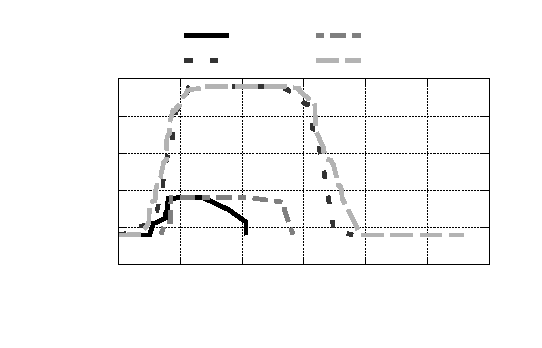
\includegraphics{rule}}%
    \gplfronttext
  \end{picture}%
\endgroup
}
    \caption{P4, fat-tree, 100 path changes}
    \label{fig:rule_number:fat_tree}
  \end{subfigure}
  \begin{subfigure}[b]{0.49\linewidth}
    \resizebox{\linewidth}{!}{\footnotesize% GNUPLOT: LaTeX picture with Postscript
\begingroup
  \fontfamily{Times-Roman}%
  \selectfont
  \makeatletter
  \providecommand\color[2][]{%
    \GenericError{(gnuplot) \space\space\space\@spaces}{%
      Package color not loaded in conjunction with
      terminal option `colourtext'%
    }{See the gnuplot documentation for explanation.%
    }{Either use 'blacktext' in gnuplot or load the package
      color.sty in LaTeX.}%
    \renewcommand\color[2][]{}%
  }%
  \providecommand\includegraphics[2][]{%
    \GenericError{(gnuplot) \space\space\space\@spaces}{%
      Package graphicx or graphics not loaded%
    }{See the gnuplot documentation for explanation.%
    }{The gnuplot epslatex terminal needs graphicx.sty or graphics.sty.}%
    \renewcommand\includegraphics[2][]{}%
  }%
  \providecommand\rotatebox[2]{#2}%
  \@ifundefined{ifGPcolor}{%
    \newif\ifGPcolor
    \GPcolortrue
  }{}%
  \@ifundefined{ifGPblacktext}{%
    \newif\ifGPblacktext
    \GPblacktexttrue
  }{}%
  % define a \g@addto@macro without @ in the name:
  \let\gplgaddtomacro\g@addto@macro
  % define empty templates for all commands taking text:
  \gdef\gplbacktext{}%
  \gdef\gplfronttext{}%
  \makeatother
  \ifGPblacktext
    % no textcolor at all
    \def\colorrgb#1{}%
    \def\colorgray#1{}%
  \else
    % gray or color?
    \ifGPcolor
      \def\colorrgb#1{\color[rgb]{#1}}%
      \def\colorgray#1{\color[gray]{#1}}%
      \expandafter\def\csname LTw\endcsname{\color{white}}%
      \expandafter\def\csname LTb\endcsname{\color{black}}%
      \expandafter\def\csname LTa\endcsname{\color{black}}%
      \expandafter\def\csname LT0\endcsname{\color[rgb]{1,0,0}}%
      \expandafter\def\csname LT1\endcsname{\color[rgb]{0,1,0}}%
      \expandafter\def\csname LT2\endcsname{\color[rgb]{0,0,1}}%
      \expandafter\def\csname LT3\endcsname{\color[rgb]{1,0,1}}%
      \expandafter\def\csname LT4\endcsname{\color[rgb]{0,1,1}}%
      \expandafter\def\csname LT5\endcsname{\color[rgb]{1,1,0}}%
      \expandafter\def\csname LT6\endcsname{\color[rgb]{0,0,0}}%
      \expandafter\def\csname LT7\endcsname{\color[rgb]{1,0.3,0}}%
      \expandafter\def\csname LT8\endcsname{\color[rgb]{0.5,0.5,0.5}}%
    \else
      % gray
      \def\colorrgb#1{\color{black}}%
      \def\colorgray#1{\color[gray]{#1}}%
      \expandafter\def\csname LTw\endcsname{\color{white}}%
      \expandafter\def\csname LTb\endcsname{\color{black}}%
      \expandafter\def\csname LTa\endcsname{\color{black}}%
      \expandafter\def\csname LT0\endcsname{\color{black}}%
      \expandafter\def\csname LT1\endcsname{\color{black}}%
      \expandafter\def\csname LT2\endcsname{\color{black}}%
      \expandafter\def\csname LT3\endcsname{\color{black}}%
      \expandafter\def\csname LT4\endcsname{\color{black}}%
      \expandafter\def\csname LT5\endcsname{\color{black}}%
      \expandafter\def\csname LT6\endcsname{\color{black}}%
      \expandafter\def\csname LT7\endcsname{\color{black}}%
      \expandafter\def\csname LT8\endcsname{\color{black}}%
    \fi
  \fi
    \setlength{\unitlength}{0.0500bp}%
    \ifx\gptboxheight\undefined%
      \newlength{\gptboxheight}%
      \newlength{\gptboxwidth}%
      \newsavebox{\gptboxtext}%
    \fi%
    \setlength{\fboxrule}{0.5pt}%
    \setlength{\fboxsep}{1pt}%
\begin{picture}(4896.00,3024.00)%
    \gplgaddtomacro\gplbacktext{%
      \csname LTb\endcsname%%
      \put(980,640){\makebox(0,0)[r]{\strut{}$13800$}}%
      \csname LTb\endcsname%%
      \put(980,937){\makebox(0,0)[r]{\strut{}$14100$}}%
      \csname LTb\endcsname%%
      \put(980,1234){\makebox(0,0)[r]{\strut{}$14400$}}%
      \csname LTb\endcsname%%
      \put(980,1532){\makebox(0,0)[r]{\strut{}$14700$}}%
      \csname LTb\endcsname%%
      \put(980,1829){\makebox(0,0)[r]{\strut{}$15000$}}%
      \csname LTb\endcsname%%
      \put(980,2126){\makebox(0,0)[r]{\strut{}$15300$}}%
      \csname LTb\endcsname%%
      \put(980,2423){\makebox(0,0)[r]{\strut{}$15600$}}%
      \csname LTb\endcsname%%
      \put(1100,440){\makebox(0,0){\strut{}$0$}}%
      \csname LTb\endcsname%%
      \put(1787,440){\makebox(0,0){\strut{}$0.5$}}%
      \csname LTb\endcsname%%
      \put(2474,440){\makebox(0,0){\strut{}$1$}}%
      \csname LTb\endcsname%%
      \put(3161,440){\makebox(0,0){\strut{}$1.5$}}%
      \csname LTb\endcsname%%
      \put(3848,440){\makebox(0,0){\strut{}$2$}}%
      \csname LTb\endcsname%%
      \put(4535,440){\makebox(0,0){\strut{}$2.5$}}%
    }%
    \gplgaddtomacro\gplfronttext{%
      \csname LTb\endcsname%%
      \put(420,1531){\rotatebox{-270}{\makebox(0,0){\strut{}The total number of rules}}}%
      \put(2817,140){\makebox(0,0){\strut{}Time (s)}}%
      \csname LTb\endcsname%%
      \put(2217,2841){\makebox(0,0)[l]{\strut{}\sys}}%
      \csname LTb\endcsname%%
      \put(2217,2601){\makebox(0,0)[l]{\strut{}\cu}}%
      \csname LTb\endcsname%%
      \put(3480,2841){\makebox(0,0)[l]{\strut{}\tsu}}%
      \csname LTb\endcsname%%
      \put(3480,2601){\makebox(0,0)[l]{\strut{}\coconut}}%
    }%
    \gplbacktext
    \put(0,0){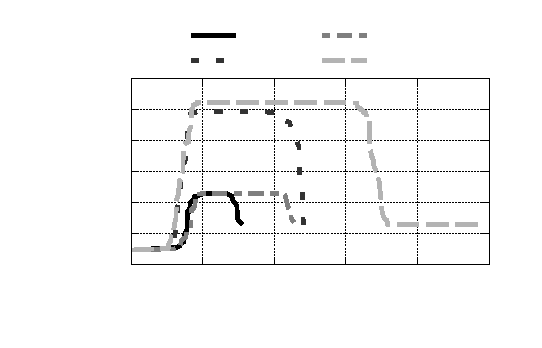
\includegraphics{isprule}}%
    \gplfronttext
  \end{picture}%
\endgroup
}
    \caption{P4, DFN, 306 path changes}
    \label{fig:rule_number:dfn}
  \end{subfigure}
\caption{Rules in the network during epoch installation.}
\label{fig:rule_number}
\end{figure}


\subsection{Rule Generation Time}
\label{sec:eval:rulegen}

Rule generation times for SCC are shown in \figref{fig:rulegen}.
There are two groups of box-plots shown in \figref{fig:rulegen}: one
for fat-tree topologies, and one for ISP topologies.  Of the listed
ISP topologies, the two numbers following each topology name (e.g.,
``40'' and ``61'' in ``Geant2012(40,61)'') are the number of switches
and links in the topology, respectively.  The numbers
in \figref{fig:rulegen} for the fat-tree topologies are
rule-generation times where the new epoch differs from the old epoch
by a sequence of 100 route changes present in the Facebook data (as
in \figref{fig:rule_number}).  The experiments with ISP topologies
reflect the cost of rule generation when a random link fails, causing
all routes traversing it to change.

\begin{figure}
\centering
  \resizebox{0.49\linewidth}{!}{% GNUPLOT: LaTeX picture with Postscript
\begingroup
  \fontfamily{Times-Roman}%
  \selectfont
  \makeatletter
  \providecommand\color[2][]{%
    \GenericError{(gnuplot) \space\space\space\@spaces}{%
      Package color not loaded in conjunction with
      terminal option `colourtext'%
    }{See the gnuplot documentation for explanation.%
    }{Either use 'blacktext' in gnuplot or load the package
      color.sty in LaTeX.}%
    \renewcommand\color[2][]{}%
  }%
  \providecommand\includegraphics[2][]{%
    \GenericError{(gnuplot) \space\space\space\@spaces}{%
      Package graphicx or graphics not loaded%
    }{See the gnuplot documentation for explanation.%
    }{The gnuplot epslatex terminal needs graphicx.sty or graphics.sty.}%
    \renewcommand\includegraphics[2][]{}%
  }%
  \providecommand\rotatebox[2]{#2}%
  \@ifundefined{ifGPcolor}{%
    \newif\ifGPcolor
    \GPcolortrue
  }{}%
  \@ifundefined{ifGPblacktext}{%
    \newif\ifGPblacktext
    \GPblacktexttrue
  }{}%
  % define a \g@addto@macro without @ in the name:
  \let\gplgaddtomacro\g@addto@macro
  % define empty templates for all commands taking text:
  \gdef\gplbacktext{}%
  \gdef\gplfronttext{}%
  \makeatother
  \ifGPblacktext
    % no textcolor at all
    \def\colorrgb#1{}%
    \def\colorgray#1{}%
  \else
    % gray or color?
    \ifGPcolor
      \def\colorrgb#1{\color[rgb]{#1}}%
      \def\colorgray#1{\color[gray]{#1}}%
      \expandafter\def\csname LTw\endcsname{\color{white}}%
      \expandafter\def\csname LTb\endcsname{\color{black}}%
      \expandafter\def\csname LTa\endcsname{\color{black}}%
      \expandafter\def\csname LT0\endcsname{\color[rgb]{1,0,0}}%
      \expandafter\def\csname LT1\endcsname{\color[rgb]{0,1,0}}%
      \expandafter\def\csname LT2\endcsname{\color[rgb]{0,0,1}}%
      \expandafter\def\csname LT3\endcsname{\color[rgb]{1,0,1}}%
      \expandafter\def\csname LT4\endcsname{\color[rgb]{0,1,1}}%
      \expandafter\def\csname LT5\endcsname{\color[rgb]{1,1,0}}%
      \expandafter\def\csname LT6\endcsname{\color[rgb]{0,0,0}}%
      \expandafter\def\csname LT7\endcsname{\color[rgb]{1,0.3,0}}%
      \expandafter\def\csname LT8\endcsname{\color[rgb]{0.5,0.5,0.5}}%
    \else
      % gray
      \def\colorrgb#1{\color{black}}%
      \def\colorgray#1{\color[gray]{#1}}%
      \expandafter\def\csname LTw\endcsname{\color{white}}%
      \expandafter\def\csname LTb\endcsname{\color{black}}%
      \expandafter\def\csname LTa\endcsname{\color{black}}%
      \expandafter\def\csname LT0\endcsname{\color{black}}%
      \expandafter\def\csname LT1\endcsname{\color{black}}%
      \expandafter\def\csname LT2\endcsname{\color{black}}%
      \expandafter\def\csname LT3\endcsname{\color{black}}%
      \expandafter\def\csname LT4\endcsname{\color{black}}%
      \expandafter\def\csname LT5\endcsname{\color{black}}%
      \expandafter\def\csname LT6\endcsname{\color{black}}%
      \expandafter\def\csname LT7\endcsname{\color{black}}%
      \expandafter\def\csname LT8\endcsname{\color{black}}%
    \fi
  \fi
    \setlength{\unitlength}{0.0500bp}%
    \ifx\gptboxheight\undefined%
      \newlength{\gptboxheight}%
      \newlength{\gptboxwidth}%
      \newsavebox{\gptboxtext}%
    \fi%
    \setlength{\fboxrule}{0.5pt}%
    \setlength{\fboxsep}{1pt}%
\begin{picture}(5760.00,3168.00)%
    \gplgaddtomacro\gplbacktext{%
      \csname LTb\endcsname%
      \put(484,1112){\makebox(0,0)[r]{\strut{}$0$}}%
      \csname LTb\endcsname%
      \put(484,1609){\makebox(0,0)[r]{\strut{}$1$}}%
      \csname LTb\endcsname%
      \put(484,2107){\makebox(0,0)[r]{\strut{}$2$}}%
      \csname LTb\endcsname%
      \put(484,2604){\makebox(0,0)[r]{\strut{}$3$}}%
      \csname LTb\endcsname%
      \put(484,3101){\makebox(0,0)[r]{\strut{}$4$}}%
      \csname LTb\endcsname%
      \put(1080,980){\rotatebox{25}{\makebox(0,0)[r]{\strut{}Abilene(11,14)}}}%
      \csname LTb\endcsname%
      \put(1682,980){\rotatebox{25}{\makebox(0,0)[r]{\strut{}Quest(20,31)}}}%
      \csname LTb\endcsname%
      \put(2284,980){\rotatebox{25}{\makebox(0,0)[r]{\strut{}Arnes(34,47)}}}%
      \csname LTb\endcsname%
      \put(2886,980){\rotatebox{25}{\makebox(0,0)[r]{\strut{}Geant2012(40,61)}}}%
      \csname LTb\endcsname%
      \put(3488,980){\rotatebox{25}{\makebox(0,0)[r]{\strut{}Dfn(58,87)}}}%
      \csname LTb\endcsname%
      \put(4692,980){\rotatebox{25}{\makebox(0,0)[r]{\strut{}FatTree(K=6)}}}%
      \csname LTb\endcsname%
      \put(5294,980){\rotatebox{25}{\makebox(0,0)[r]{\strut{}FatTree(K=8)}}}%
    }%
    \gplgaddtomacro\gplfronttext{%
      \csname LTb\endcsname%
      \put(176,2106){\rotatebox{-270}{\makebox(0,0){\strut{}Time (s)}}}%
    }%
    \gplgaddtomacro\gplbacktext{%
      \csname LTb\endcsname%
      \put(4081,1822){\makebox(0,0)[r]{\strut{}0.04}}%
      \put(4081,2297){\makebox(0,0)[r]{\strut{}0.06}}%
      \put(4081,2772){\makebox(0,0)[r]{\strut{}0.08}}%
    }%
    \gplgaddtomacro\gplfronttext{%
    }%
    \gplbacktext
    \put(0,0){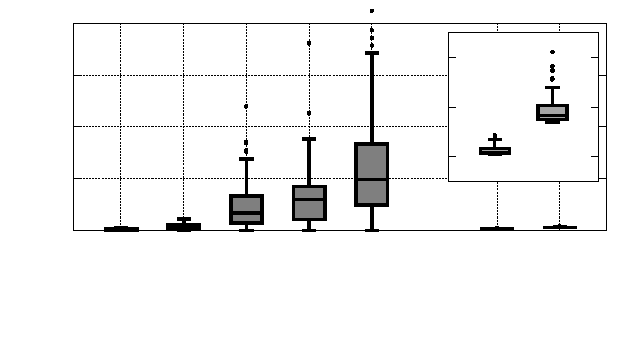
\includegraphics{boxperf}}%
    \gplfronttext
  \end{picture}%
\endgroup
}
  \caption{Distributions of SCC rule-generation times (100 path
  updates in fat-tree topologies; random link failure in ISP
  topologies).}
  \label{fig:rulegen}
\end{figure}


\figref{fig:rulegen} shows distributions of rule-generation times
as box-plots.  Each box shows the first, second (median),
and third quartiles, and whiskers extend to cover points that fall
within $1.5\times$ the interquartile range.  Outliers are shown as
dots.

Rule-generation times were minimal for the fat-tree topologies, even
for epochs modifying 100 routing paths.  Rule
generation times for ISP topologies were more substantial, but
typically completed in under $1\secs$ for all but one topology (DFN).
Rule generation for DFN rarely exceeded $3\secs$, but in these cases,
the link failure induced changes in over 250 routes.  While we
are encouraged by these results, there are numerous opportunities for
optimization in our current codebase (e.g., parallelization).

\subsection{Buffer Overhead}
\label{sec:eval:buffer}

\begin{figure}
\centering
  \resizebox{0.49\linewidth}{!}{% GNUPLOT: LaTeX picture with Postscript
\begingroup
  \fontfamily{Times-Roman}%
  \selectfont
  \makeatletter
  \providecommand\color[2][]{%
    \GenericError{(gnuplot) \space\space\space\@spaces}{%
      Package color not loaded in conjunction with
      terminal option `colourtext'%
    }{See the gnuplot documentation for explanation.%
    }{Either use 'blacktext' in gnuplot or load the package
      color.sty in LaTeX.}%
    \renewcommand\color[2][]{}%
  }%
  \providecommand\includegraphics[2][]{%
    \GenericError{(gnuplot) \space\space\space\@spaces}{%
      Package graphicx or graphics not loaded%
    }{See the gnuplot documentation for explanation.%
    }{The gnuplot epslatex terminal needs graphicx.sty or graphics.sty.}%
    \renewcommand\includegraphics[2][]{}%
  }%
  \providecommand\rotatebox[2]{#2}%
  \@ifundefined{ifGPcolor}{%
    \newif\ifGPcolor
    \GPcolortrue
  }{}%
  \@ifundefined{ifGPblacktext}{%
    \newif\ifGPblacktext
    \GPblacktexttrue
  }{}%
  % define a \g@addto@macro without @ in the name:
  \let\gplgaddtomacro\g@addto@macro
  % define empty templates for all commands taking text:
  \gdef\gplbacktext{}%
  \gdef\gplfronttext{}%
  \makeatother
  \ifGPblacktext
    % no textcolor at all
    \def\colorrgb#1{}%
    \def\colorgray#1{}%
  \else
    % gray or color?
    \ifGPcolor
      \def\colorrgb#1{\color[rgb]{#1}}%
      \def\colorgray#1{\color[gray]{#1}}%
      \expandafter\def\csname LTw\endcsname{\color{white}}%
      \expandafter\def\csname LTb\endcsname{\color{black}}%
      \expandafter\def\csname LTa\endcsname{\color{black}}%
      \expandafter\def\csname LT0\endcsname{\color[rgb]{1,0,0}}%
      \expandafter\def\csname LT1\endcsname{\color[rgb]{0,1,0}}%
      \expandafter\def\csname LT2\endcsname{\color[rgb]{0,0,1}}%
      \expandafter\def\csname LT3\endcsname{\color[rgb]{1,0,1}}%
      \expandafter\def\csname LT4\endcsname{\color[rgb]{0,1,1}}%
      \expandafter\def\csname LT5\endcsname{\color[rgb]{1,1,0}}%
      \expandafter\def\csname LT6\endcsname{\color[rgb]{0,0,0}}%
      \expandafter\def\csname LT7\endcsname{\color[rgb]{1,0.3,0}}%
      \expandafter\def\csname LT8\endcsname{\color[rgb]{0.5,0.5,0.5}}%
    \else
      % gray
      \def\colorrgb#1{\color{black}}%
      \def\colorgray#1{\color[gray]{#1}}%
      \expandafter\def\csname LTw\endcsname{\color{white}}%
      \expandafter\def\csname LTb\endcsname{\color{black}}%
      \expandafter\def\csname LTa\endcsname{\color{black}}%
      \expandafter\def\csname LT0\endcsname{\color{black}}%
      \expandafter\def\csname LT1\endcsname{\color{black}}%
      \expandafter\def\csname LT2\endcsname{\color{black}}%
      \expandafter\def\csname LT3\endcsname{\color{black}}%
      \expandafter\def\csname LT4\endcsname{\color{black}}%
      \expandafter\def\csname LT5\endcsname{\color{black}}%
      \expandafter\def\csname LT6\endcsname{\color{black}}%
      \expandafter\def\csname LT7\endcsname{\color{black}}%
      \expandafter\def\csname LT8\endcsname{\color{black}}%
    \fi
  \fi
    \setlength{\unitlength}{0.0500bp}%
    \ifx\gptboxheight\undefined%
      \newlength{\gptboxheight}%
      \newlength{\gptboxwidth}%
      \newsavebox{\gptboxtext}%
    \fi%
    \setlength{\fboxrule}{0.5pt}%
    \setlength{\fboxsep}{1pt}%
\begin{picture}(5760.00,3456.00)%
    \gplgaddtomacro\gplbacktext{%
      \csname LTb\endcsname%
      \put(682,707){\makebox(0,0)[r]{\strut{}$0$}}%
      \csname LTb\endcsname%
      \put(682,1378){\makebox(0,0)[r]{\strut{}$200$}}%
      \csname LTb\endcsname%
      \put(682,2048){\makebox(0,0)[r]{\strut{}$400$}}%
      \csname LTb\endcsname%
      \put(682,2719){\makebox(0,0)[r]{\strut{}$600$}}%
      \csname LTb\endcsname%
      \put(682,3389){\makebox(0,0)[r]{\strut{}$800$}}%
      \csname LTb\endcsname%
      \put(1555,575){\rotatebox{25}{\makebox(0,0)[r]{\strut{}600}}}%
      \csname LTb\endcsname%
      \put(2437,575){\rotatebox{25}{\makebox(0,0)[r]{\strut{}700}}}%
      \csname LTb\endcsname%
      \put(3319,575){\rotatebox{25}{\makebox(0,0)[r]{\strut{}800}}}%
      \csname LTb\endcsname%
      \put(4201,575){\rotatebox{25}{\makebox(0,0)[r]{\strut{}900}}}%
      \csname LTb\endcsname%
      \put(5083,575){\rotatebox{25}{\makebox(0,0)[r]{\strut{}1000}}}%
    }%
    \gplgaddtomacro\gplfronttext{%
      \csname LTb\endcsname%
      \put(176,2048){\rotatebox{-270}{\makebox(0,0){\strut{}Number of buffered packets}}}%
      \put(3372,154){\makebox(0,0){\strut{}Packets per second}}%
    }%
    \gplbacktext
    \put(0,0){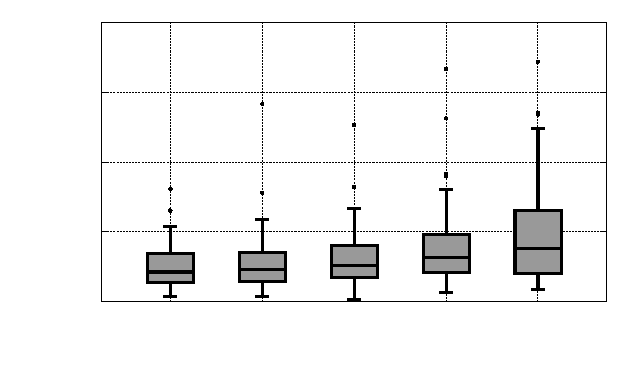
\includegraphics{buffer}}%
    \gplfronttext
  \end{picture}%
\endgroup
}
  \caption{Distributions of SCC maximum switch buffering during 10 path
  updates in fat-tree ($\portsPerSwitch = 8$).}
  \label{fig:buffer}
\end{figure}

In the tests reported in this section, we measured the peak number of
buffered packets on any switch, for different packet sending
rates. Each epoch in these tests involved ten path changes,
and \figref{fig:buffer} shows the distribution of the maximum number
of simultaneously buffered packets at any switch for 100 such epochs
for the fat-tree topology ($\portsPerSwitch = 8$).  As shown in the
figure, the number of buffered packets per switch rarely exceeded 200
and the buffering grew linearly as a function of packet sending rate.
Buffer sizes of commodity switches are usually in the $\megabytes$ or
even $\gigabytes$ range~\cite{buffer},
and so these buffering obligations should not be problematic.

\chapter{\uppercase{Nimble: Fast and Safe Migration of Network Functions}}
\label{chap:nimble}
\graphicspath{{./}{./fig/}{./fig/nimble/}}

Stateful network functions (NFs) are a staple of modern network
infrastructures.  For example, network intrusion detection/prevention systems (NIDS/NIPS) is critical to ensure network security. However, the
consequences of missing packets can be significant, and methods to
sneak attacks past NIDS/NIPS to destination targets have a long
history (e.g.,~\cite{chaboya2006:network, cheng2012:evasion,
  corona2013:adversarial}). The risk of traffic sidestepping intended NFs is particularly acute
during routing-policy updates.  Even if NFs remain in the same place
during the update, packets that transition from a point upstream of
the NF on the old routing path to a point downstream from the NF on
the new routing path can result in an NF missing these packets.
Routing-policy update algorithms that ensure \textit{consistent
  update} (e.g.,~\cite{CU, tsu}) can guarantee that all traffic
gets processed (again, when the NF doesn't itself move), for example
by ensuring that each packet traverses either its old path in its
entirety or its new path in its entirety.

In this chapter, we provide a method and accompanying implementation,
called \sysname, for interleaving routing-policy update and NF
migration in a software-defined network (SDN), in a way that
significantly reduces the latency to achieve both and without
permitting packets to evade processing by NFs.  Our technique works
with any route-update protocol that implements a property we call
\textit{relaxed waypoint correctness}, which includes
consistent-update protocols like CU~\cite{CU} and our SCC algorithm.
However, we provide a route-update protocol that is customized to
achieve relaxed waypoint correctness without conforming to
conventional ``consistent update'' semantics, as typically defined for
such protocols.

As we will show, permitting both routing updates and NF migrations to
proceed concurrently is a delicate endeavor that is fraught with
corner cases.  To holistically address these cases while synchronizing
these tasks as little as possible, \sysname leverages targeted
buffering and packet marking in the network to coordinate packet
processing with NF migration.  The benefits to this approach are
myriad, however, including lower latency for completion of both tasks
and, depending on the routing-update protocol with which NF migration
is being deployed and the circumstances requiring their update,
reduced packet loss and/or reduced rule overhead in switches.

We have implemented \sysname on Open vSwitch~\cite{ovs} and the Ryu
controller~\cite{ryu}.  We evaluate implementations of \sysname
building on both CU~\cite{CU} and SCC, as well as a
route-update protocol of our own design to satisfy specifically the
relaxed waypoint correctness property that we define.  We empirically
compare our implementations of \sysname to OpenNF~\cite{opennf} and
SwingState~\cite{swingstate}, and demonstrate the benefits of our
design in both FatTree and ISP topologies.


\section{Framework and Goals}
\label{sec:goals}

\subsection{SDN Model}
\label{sec:goals:network}

We adopt an SDN model, in which a \textit{controller} deploys
\textit{rules} to distributed \textit{switches} to implement routing
policy.

\paragraph{Flows}
As is standard, we define a \textit{flow} to consist of packets with
the same addressing information, i.e., IP 5-tuple.  The space of all
possible such 5-tuples, and so the space of all flows, is
denoted \flowSpace.  We denote by $\subFlowSpace \subset \flowSpace$
the space of possible flows between switches or between a switch and
the controller.  When convenient, we treat a flow \flowID{} as a set
of all possible packets with addressing information defined by
\flowID{} and use $\pktID{} \in \flowID{}$ to denote a packet \pktID{}
with the addressing information of \flowID{}.

\paragraph{Controller}
The network has a logically centralized controller that is responsible
for configuring the switches to update the route of each flow.  The
controller executes an SDN application consisting of a \textit{route
  generator} and an \textit{update scheduler}.  The route generator
decides whether to change the routes of flows by monitoring the
network conditions and topology changes. The output of the route
generator is the routing path of each flow \flowID{}.

The SDN update scheduler produces \textit{rules} (defined below) to be
deployed on each switch, and to schedule these switch updates to
preserve certain network routing properties when transitioning from
the old routing policies to the new.  Specifically, the update
scheduler outputs a schedule of rule deployment in \updateSteps steps,
denoted as $\updateID{1}, \updateID{2}, ...,
\updateID{\updateSteps}$. Each \updateID{\updateIdx} includes a set of
\flowAdd and \flowDel commands to add or remove rules on switches; we
discuss these commands and the structure of rules below. The commands
in \updateID{\updateIdx} are issued simultaneously to switches in the
network, and updates of \updateID{\updateIdx} are finished before
\updateID{\updateIdx+1} begins.

We refer to an invocation of the SDN application to reconfigure
routing policy as a new \textit{epoch}.  We assume that each routing
policy change completes---i.e., its rules are deployed throughout the
network---before the next epoch begins.

\paragraph{Switches}
Similiar to the switch model for SCC algorithm in \chapref{chap:scc}, each switch maintains a flow entry table which stores a set of rules
(see below) for flow management.  We denote the set of rules in the
flow table of switch \switchID{} as \switchID{}{\ruleSet}; e.g.,
$\switchID{}{\ruleSet} = \{\ruleID{1}, \ruleID{6}, \ruleID{10}\}$
means that switch \switchID{} includes rules $\ruleID{1}$,
$\ruleID{6}$ and $\ruleID{10}$.  The controller modifies this set by
invoking the following interface, which is similar to that provided by
OpenFlow:
\begin{itemize}[nosep,leftmargin=1em,labelwidth=*,align=left]
\item
\switchID{}{\flowAdd{\ruleID{\ruleIdx}}} inserts rule
\ruleID{\ruleIdx} into \switchID{}{\ruleSet}.  This command fails with
no effect if $\ruleID{\ruleIdx}{\switchField} \neq \switchID{}$ (i.e., \ruleID{\ruleIdx} should not be installed at \switchID{}) or if
\switchID{}{\ruleSet} already contains a rule \ruleID{\ruleIdxAlt}
such that $\ruleID{\ruleIdxAlt}{\priorityField} =
\ruleID{\ruleIdx}{\priorityField}$, $\ruleID{\ruleIdxAlt}{\coverField}
\cap \ruleID{\ruleIdx}{\coverField} \neq \emptyset$ (i.e., some packets can be matched by both \ruleID{\ruleIdx} and \ruleID{\ruleIdxAlt}).  The meanings of
these rule fields are described below.
\item \switchID{}{\flowDel{\ruleID{\ruleIdx}}} removes rule
  \ruleID{\ruleIdx} from \switchID{}{\ruleSet}.
\end{itemize}
We assume that switches support \textit{bundling}, i.e., that a set of
invocations from the controller will collectively be performed as a
single atomic transaction with respect to packet processing by the
switch.

\paragraph{Rules}
The instructions for how a switch should treat packets are specified
by \textit{rules}.  When a packet arrives at a switch, it can be
\textit{matched} to at most one rule installed on the switch, which
determines what happens to the packet.  Similiar to the definition of rules in \chapref{chap:scc}, each rule \ruleID{} includes
(at least) the following fields, all of which are immutable:
\begin{itemize}[nosep,leftmargin=1em,labelwidth=*,align=left]
\item \ruleID{}{\switchField{}} specifies the unique switch
  \switchID{} into which \ruleID{} can be installed.

\item \ruleID{}{\priorityField} specifies the priority of this rule,
  with higher priorities indicated by larger numbers, and with a
  special priority $\infty$ to represent the maximum priority, which
  can be used only by our algorithm;

\item $\ruleID{}{\coverField} \subseteq \flowSpace$ specifies the
  flows to which this rule can be matched, i.e., a packet \pktID{} can
  be matched to \ruleID{} only if $\flowID{} \in
  \ruleID{}{\coverField}$ for the flow \flowID{} containing \pktID{}.

\item \ruleID{}{\sendToField} specifies the switch identifier (in
  practice, an outbound port) to which packets matched to this rule
  should be forwarded.  If \ruleID{}{\sendToField} is switch
  \switchID{\switchIdx}, then there must be a link between
  \ruleID{}{\switchField{}} and \switchID{\switchIdx}.
\end{itemize}

\subsection{Network Functions}
\label{sec:goals:correctness}

Our goal is to extend the SDN model described above to support
\textit{network functions}.  Below we describe the form of these
network functions and the basic correctness requirement we have for
their traversal.

\paragraph{Network functions}
A \textit{network function} \nfID{\nfIdx} is an object with an
immutable field \\
$\nfID{\nfIdx}{}{\flowSpec} \subseteq \flowSpace$ and
a method \nfID{\nfIdx}{}{\processPkt} that takes as input a packet
\pktID{} in some $\flowID{} \in \nfID{\nfIdx}{}{\flowSpec}$ and
outputs a (possibly empty) set of packets \pktSet{}, also in
\flowID{}.  If \pktID{} is part of a flow $\flowID{} \not\in
\nfID{\nfIdx}{}{\flowSpec}$, then
\nfID{\nfIdx}{}{\processPkt{\pktID{}}} has no effect.  Correctness of
\nfID{\nfIdx} is defined by a \textit{sequential specification} that
specifies its correct behavior when \nfID{\nfIdx}{}{\processPkt} is
invoked sequentially, i.e., so that each method invocation returns
before the next invocation begins, and that execution of
\nfID{\nfIdx}{}{\processPkt} is
linearizable~\cite{herlihy1990:linearizability}.  Let \nfNmbr be the
number of network functions; i.e., the network functions are \nfID{1},
$\ldots$, \nfID{\nfNmbr}.



\paragraph{Waypoint correctness}
Let $\nats{\genericNat} = \{1, \ldots, \genericNat\}$.  For each flow
\flowID{}, there is a specified injective function $\wpFn{\flowID{}}:
\nats{\wpNmbr{\flowID{}}} \rightarrow \nats{\nfNmbr}$ where
\wpNmbr{\flowID{}} is the number of network functions that should process packets of \flowID{} sequentially on the entire path ($\wpNmbr{\flowID{}} \ge 0$) and \wpFn{\flowID{}}{\wpIdx} is the
$\wpIdx$-th network function that packets in \flowID{} must traverse.
We require that if $\wpFn{\flowID{}}{\wpIdx} = \nfIdx$, then
$\flowID{} \in \nfID{\nfIdx}{}{\flowSpec}$.  Our correctness condition
is that the network enforce the waypoint property, i.e., for any
\flowID{} and any packet \pktID{} in \flowID{} that enters the
network,
\begin{itemize}[nosep,leftmargin=1em,labelwidth=*,align=left]
  \item if $\wpNmbr{\flowID{}} > 0$, then
    \nfID{\nfIdx}{}{\processPkt{\pktID{}}} is invoked for $\nfIdx =
    \wpFn{\flowID{}}{1}$;
  \item for each \wpIdx, $1 \le \wpIdx < \wpNmbr{\flowID{}}$, if
    \nfID{\nfIdx}{}{\processPkt{\pktIDAlt{}}} is invoked for $\nfIdx =
    \wpFn{\flowID{}}{\wpIdx}$, outputting \pktSet,
    then \nfID{\nfIdxAlt}{}{\processPkt{\pktIDAltAlt{}}} is invoked
    for $\nfIdxAlt = \wpFn{\flowID{}}{\wpIdx+1}$ and for every
    $\pktIDAltAlt{} \in \pktSet$;
  \item no other invocations of any network function occur except by
    the above two rules; and
  \item if \nfID{\nfIdx}{}{\processPkt{\pktIDAlt{}}} is invoked for
    $\nfIdx = \wpFn{\flowID{}}{\wpNmbr{\flowID{}}}$, producing output
    \pktSet, then every $\pktIDAltAlt{} \in \pktSet$ is forwarded to
    its destination.
\end{itemize}
The first condition guarantees that if packets of \flowID{} need to be processed by at least one network function, they must be processed by the first NF \wpFn{\flowID{}}{1}. Together with the first condition, the second condition ensures that packets of \flowID{} are processed by network functions sequentially. The third condition prevents packets from being processed by network functions that are not specified. We use the last condition to guarantee the delivery of packets to the destination.
Let $\wpNmbrMax = \max_{\flowID{}} \wpNmbr{\flowID{}}$, i.e.,
\wpNmbrMax is the maximum number of waypoints that any flow can be
required to traverse.


\section{Migratable Network Functions}
\label{sec:migration}

Our framework uses an existing SDN route-update algorithm to generate
rules and schedules to update routing policy.  Specifically, with new
routing policies as input, the route-update algorithm generates a
schedule of rule deployment to update switches.  Most prior works on
SDN routing-policy updates that achieve waypoint enforcement
(e.g.,~\cite{CU, tsu, gnu}) do so assuming that NFs remain at fixed
locations of the network during the routing-policy update.  On the
contrary, here we allow NF locations to change from one epoch to the
next, and our contribution lies in ensuring that waypoint enforcement
continues to hold.

Several works (e.g.,~\cite{split, transfer, swingstate}) have explored
the possibility of migrating network functions in concert with
routing-policy updates.  A strength of these approaches is that they
make no assumptions regarding properties of the underlying
route-update algorithm, except that it eventually deploys the rules to
faithfully implement routing policies.  However, because these
NF-migration algorithms must tolerate any transitory behavior of the
underlying route-update algorithm, they necessarily must be
conservative in how they migrate NFs, to ensure that no packets bypass
their NF waypoints while the routing policy is updated.  In fact, for
this reason, all of them permit routing-policy updates to proceed only
after all NF migrations have completed.

\begin{figure}
\centering
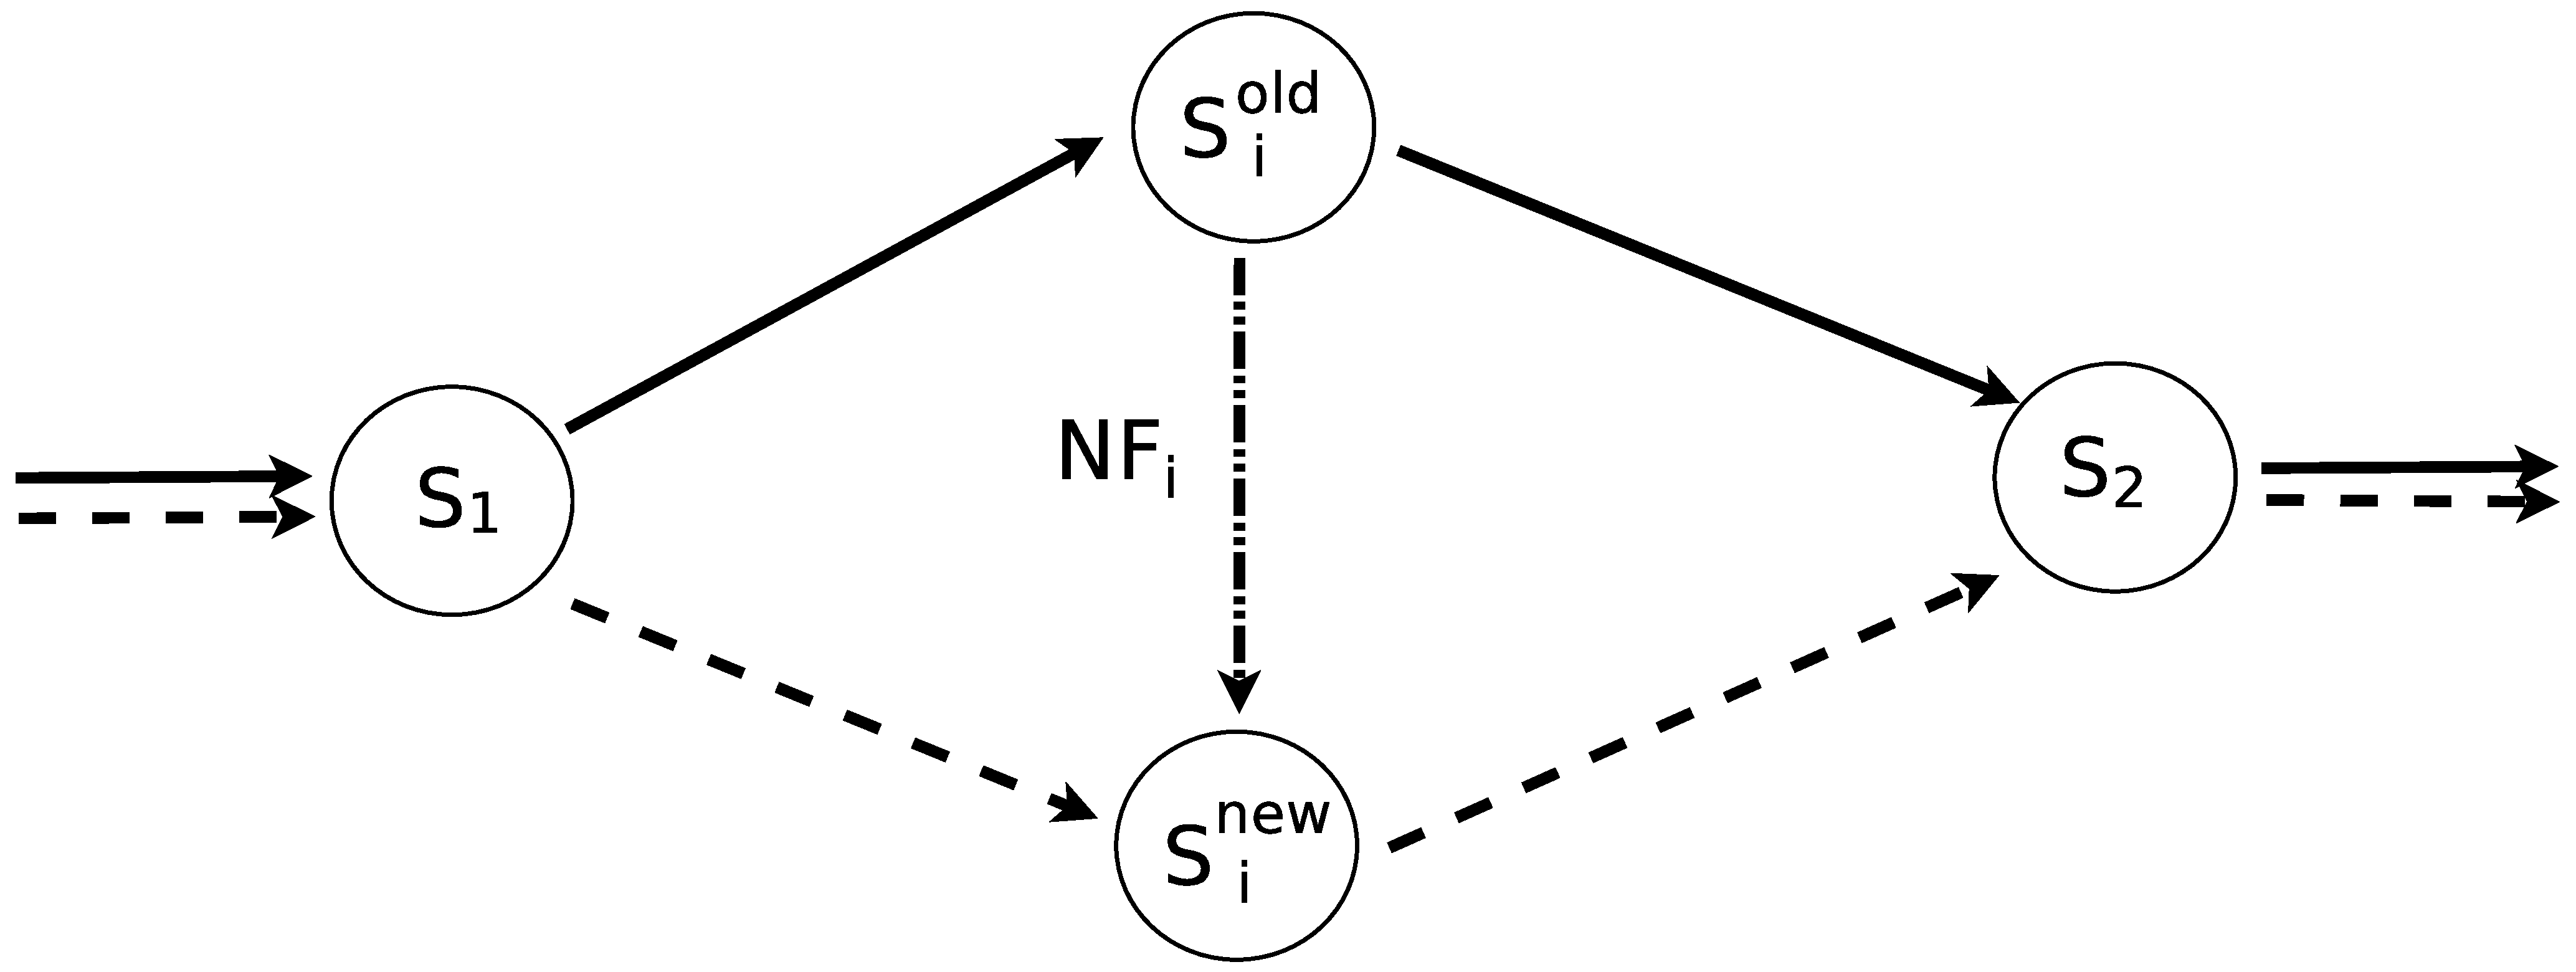
\includegraphics[width=0.85\textwidth]{basicExample.eps}
\vspace{-0.3cm}
\caption{Example of NF migration}
\label{fig:nfexample}
\vspace{-0.5cm}
\end{figure}

To understand the challenges in permitting migration alongside route
updates, consider a network function \nfID{\nfIdx} that migrates from
the old position \oldSwitchID{\nfIdx} to the new position
\newSwitchID{\nfIdx}, shown in \figref{fig:nfexample}.  The flow \flowID{}, which should be processed
by \nfID{\nfIdx}, also needs its path to be updated from $\switchID{1}
\rightarrow \oldSwitchID{\nfIdx} \rightarrow \switchID{2}$ to
$\switchID{1} \rightarrow \newSwitchID{\nfIdx} \rightarrow
\switchID{2}$. The path change can be accomplished by updating the
rule matched to \flowID{} at \switchID{1}. Migrating \nfID{\nfIdx} and
updating the path of \flowID{} without coordination can be harmful,
however. For example, if the controller sends commands to migrate
\nfID{\nfIdx} and updates \switchID{1} simultaneously, \switchID{1}
might be updated before \nfID{\nfIdx} migrates to
\newSwitchID{\nfIdx}. Then, packets of \flowID{} might start to arrive
at \newSwitchID{\nfIdx} before \nfID{\nfIdx} can process packets
there, which may cause problems since packets can bypass
\nfID{\nfIdx}. Also, if \switchID{1} has not been updated by the time
\nfID{\nfIdx} leaves \oldSwitchID{\nfIdx}, packets may arrive at
\oldSwitchID{\nfIdx} with \nfID{\nfIdx} no longer there; depending on
how \oldSwitchID{\nfIdx} handles these packets, this could result in
packet loss or packets bypassing \nfID{\nfIdx}.

Our goal is to migrate NFs and update routing-policies efficiently
while ensuring packets are processed by NFs correctly.  Specifically,
our contribution here is an algorithm that leverages consistency
properties of underlying routing-update algorithms to permit NFs to be
migrated \textit{alongside} rule deployment for new routing policies,
more efficiently than simply serializing routing-policy update after
NF migration.  In particular, our approach demonstrates that by
leveraging an SDN routing-policy update algorithm that provides a
property that we call \textit{relaxed waypoint correctness} (see
\secref{sec:schedule:condition}), we can implement waypoint
correctness when NFs are allowed to change locations much more
efficiently than known approaches to achieving both.

\subsection{Component Changes}
\label{sec:migration:components}

To support NF migration, we require that the controller, switches, and
rules be functionally enhanced in the following ways.  Below we refer
to each NF being hosted at a switch; this hosting could be implemented
on the switch for a simple NF or at an attached middlebox for a more
complex one.

\begin{figure}
\centering
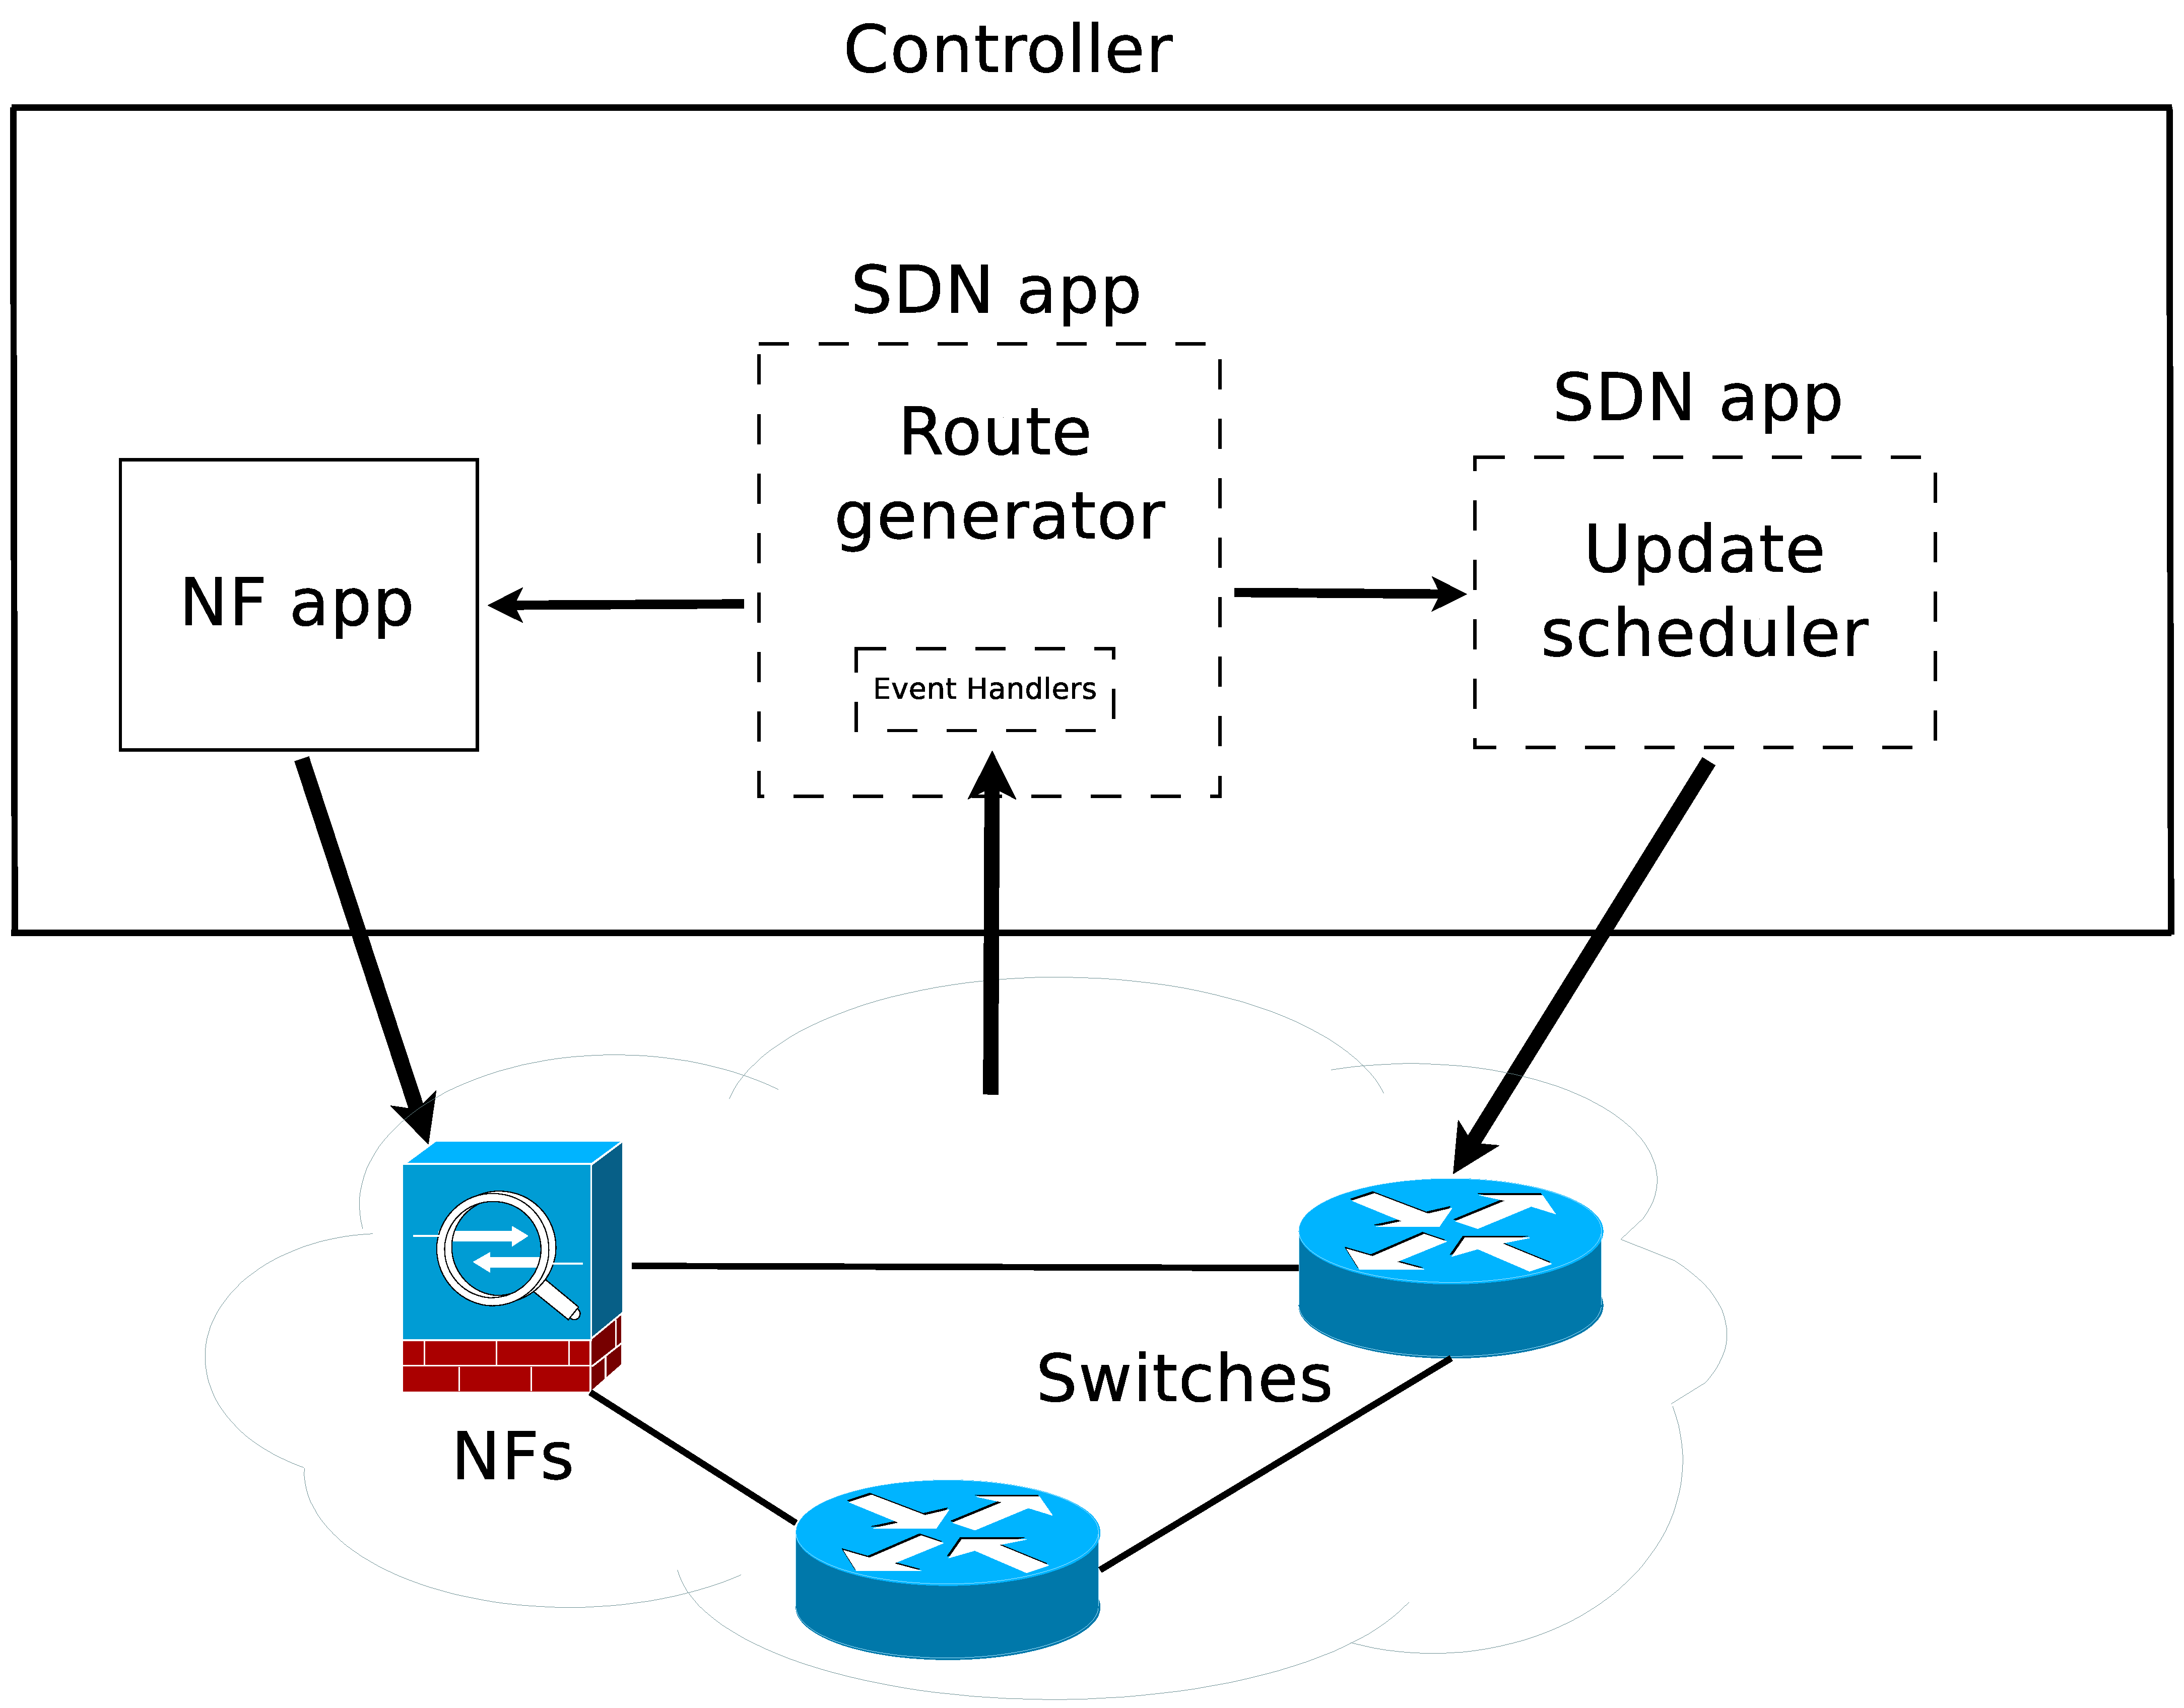
\includegraphics[width=0.8\columnwidth]{system.eps}
%\vspace{-0.3cm}
\caption{Typical components of a network controller}
\label{fig:architecture}
%\vspace{-0.5cm}
\end{figure}


\paragraph{Controller} The output from the route generator is also
provided to an NF application (see \figref{fig:architecture}), to
determine for each flow \flowID{} the switch at which \flowID{} will
be processed by each of its waypoint NFs; each NF will need to be
migrated to its corresponding switch as determined by the NF
application. It is necessary to assume that there is at least one
switch \switchID{} such that for every $\flowID{} \in
\nfID{\nfIdx}{}{\flowSpec}$, \switchID{} is included in the path of
\flowID{}, as else there is no switch to where \nfID{\nfIdx} can be
migrated to process every flow in \nfID{\nfIdx}{}{\flowSpec}.

\paragraph{Switches} We add three new switch interfaces to perform NF migration. 
\begin{itemize}[nosep,leftmargin=1em,labelwidth=*,align=left]
\item \switchID{}{\export{\nfIdx}{\switchIdx}} marshals \nfID{\nfIdx}
  into a set \pktSet of packets with source address (the IP address)
  of \switchID{} and destination address of \switchID{\switchIdx}, and
  outputs \pktSet.  \switchID{}{\export{\nfIdx}{\switchIdx}} executes
  only while no \nfID{\nfIdx}{}{\processPkt} invocations are underway
  at \switchID{}, and \switchID{} no longer permits invocations of
  \nfID{\nfIdx}{}{\processPkt} once
  \switchID{}{\export{\nfIdx}{\switchIdx}} completes.
\item \switchID{}{\import{\nfIdx}{\switchIdx}} instructs switch
  \switchID{} to await the arrival of packets \pktSet from
  \switchID{\switchIdx}, from which to reconstitute function
  \nfID{\nfIdx} locally.  This invocation causes \switchID{\switchIdx}
  to allocate two buffers, an \textit{inbound} buffer to hold packets
  to be processed in \nfID{\nfIdx}{}{\processPkt} invocations once
  \nfID{\nfIdx}{} is reconstituted locally, and an \textit{outbound}
  buffer to hold packets output from \nfID{\nfIdx}{}{\processPkt}
  invocations.  Starting from this invocation and until \nfID{\nfIdx}
  is reconstituted locally, packets matched to any $\ruleID{} \in
  \switchID{}{\ruleSet}$ for which $\ruleID{}{\sendToField} =
  \nfID{\nfIdx}{}$ (see below) are buffered in the inbound buffer for
  \nfID{\nfIdx}{}.  Packets output from \nfID{\nfIdx}{}{\processPkt}
  invocations are buffered in the outbound buffer for \nfID{\nfIdx},
  until a \switchID{}{\release{\nfIdx}} invocation.
\item \switchID{}{\release{\nfIdx}} releases the packets buffered in
  the outbound buffer for \nfID{\nfIdx} to be matched against
  \switchID{}{\ruleSet}, and disables buffering so that packets
  inbound to or outbound from \nfID{\nfIdx}{} are no longer buffered.
\end{itemize}
\switchID{}{\import}, \switchID{}{\export}, and \switchID{}{\release}
can be invoked by the controller, just like \switchID{}{\flowAdd} and
\switchID{}{\flowDel}.

\iffalse
\highlight{For example, if \nfID{2} needs to be migrated from \switchID{3} to \switchID{6}, the controller should first issue \switchID{6}{\import{2}{3}} to command \switchID{6} to wait for messages from \switchID{3}. 
Then the controller leverages the interface \switchID{3}{\export{2}{6}} to instruct \switchID{3} to create a set of packets to marshal \nfID{2} and send these packets to \switchID{6}. Upon receiving packets from \switchID{3}, \switchID{6} reconstructs \nfID{2} and starts to perform \nfID{2}{}{\processPkt} invocations. Finally, after new routing policy is enabled, the controller can issue \switchID{6}{\release{2}} command and \switchID{6} releases the buffered packets to the network.}
\fi

\paragraph{Waypoint counters}  We add to each packet a field, called its
\textit{waypoint counter}, that can hold any value in
$\nats{\wpNmbrMax+1} = \{1, \ldots, \wpNmbrMax+1\}$.  Upon arrival in
the network, a packet's ingress switch initializes the packet's
waypoint counter to $1$.  In brief, this counter is incremented in the
packet as it is submitted to each of its waypoints for processing (see
below).  In this way, rules can treat a packet differently depending
on how many of its waypoints it has already traversed.

\paragraph{Rules} We extend rules to include a new field
\ruleID{}{\wpField} that takes on a value in $\nats{\wpNmbrMax} \cup
\{\ast\}$, and stipulate that a packet can be matched to this rule
only if $\ruleID{}{\wpField} = \ast$ or the packet's waypoint counter
equals \ruleID{}{\wpField}.  As such, when packet \pktID{} in flow
\flowID{} arrives at switch \switchID{}, \pktID{} is matched to the
highest priority rule $\ruleID{} \in \switchID{}{\ruleSet}$ for which
$\flowID{} \in \ruleID{}{\coverField}$ and either $\ruleID{}{\wpField}
= \ast$ or the packet's waypoint counter equals \ruleID{}{\wpField};
we denote this rule as \ruleMatchNew{\switchID{}}{\pktID{}}.  If there is
no $\ruleID{} \in \switchID{}{\ruleSet}$ to which \pktID{} can be
matched, then \pktID{} is dropped.

We also extend rules to accommodate additional functionality
related to the \ruleID{}{\sendToField} field.
\begin{itemize}[nosep,leftmargin=1em,labelwidth=*,align=left]
\item \ruleID{}{\sendToField} can be a network function \nfID{\nfIdx},
  in which case for any packet \pktID{} it matches to \ruleID{},
  $\switchID{} = \ruleID{}{\switchField}$ increments the \pktID{}'s
  waypoint counter and then submits \pktID{} to \nfID{\nfIdx} in an
  \nfID{\nfIdx}{}{\processPkt{\pktID{}}} invocation.  If
  \nfID{\nfIdx}{} is not hosted locally at \ruleID{}{\switchField{}},
  then the packet must be buffered (in the inbound buffer for
  \nfID{\nfIdx}, see above) until it is.  Any packets returned from
  the \nfID{\nfIdx}{}{\processPkt{\pktID{}}} invocation are matched
  again to \switchID{}{\ruleSet}.  We do not require \nfID{\nfIdx} to
  process packets' waypoint counters, but we do require that any
  packets \nfID{\nfIdx}{}{\processPkt{\pktID{}}} emits bear
  the same waypoint counter as \pktID{}.
\item \ruleID{}{\sendToField} can take on two more possible values,
  namely functions \encapsulate{\flowID{}} and \decapsulate.  If a
  switch \switchID{} matches packet \pktID{} to rule $\ruleID{} \in
  \switchID{}{\ruleSet}$ where $\ruleID{}{\sendToField} =
  \encapsulate{\flowID{}}$, then the packet is encapsulated into a
  packet for flow \flowID{}, which is then resubmitted for matching
  against \switchID{}{\ruleSet} at this switch \switchID{}.  A packet
  matched to a rule $\ruleID{} \in \switchID{}{\ruleSet}$ where
  $\ruleID{}{\sendToField} = \decapsulate$ is decapsulated (i.e., the
  existing packet header is removed) and the packet contained therein
  is then resubmitted for matching against \switchID{}{\ruleSet}.
\end{itemize}
As before, all rule fields remain immutable.
\iffalse
\highlight{For example, \switchID{1} is the new location for \nfID{2} and has rules \ruleID{1}, \ruleID{2}, \ruleID{3}.
\flowID{1} matches to \ruleID{1} and $\ruleID{1}{\sendToField} = \decapsulate$. \ruleID{2} satisfies that $\flowID{2} \in \ruleID{2}{\coverField}$, $\ruleID{2}{\wpField} = 3$ and $\ruleID{2}{\sendToField} = \nfID{2}$.
\ruleID{3} satisfies that $\flowID{2} \in \ruleID{3}{\coverField}$, $\ruleID{3}{\wpField} = \ast$ and $\ruleID{3}{\sendToField} = \switchID{2}$. \ruleID{2} is of higher priority than \ruleID{3}, i.e., $\ruleID{2}{\priorityField} > \ruleID{3}{\priorityField}$. Say \switchID{1} receives a packet \pktID{1} of \flowID{1}. \switchID{1} decapsulates \pktID{1} to \pktID{2} of \flowID{2}, since \pktID{1} matches to \ruleID{1}. Assume \pktID{2} carries waypoint counter $3$. Then \switchID{1} resubmits \pktID{2} to the rule table and executes the action of \ruleID{2}. \pktID{2} is sent to \nfID{2} and its waypoint counter is increased to $4$. Therefore, when \switchID{1} processes \pktID{2} again, \pktID{2} matches to \ruleID{3} and is forwarded to \switchID{2}.
}
\fi

\subsection{Algorithm}
\label{sec:migration:algo}

\begin{figure}[t]
\centering
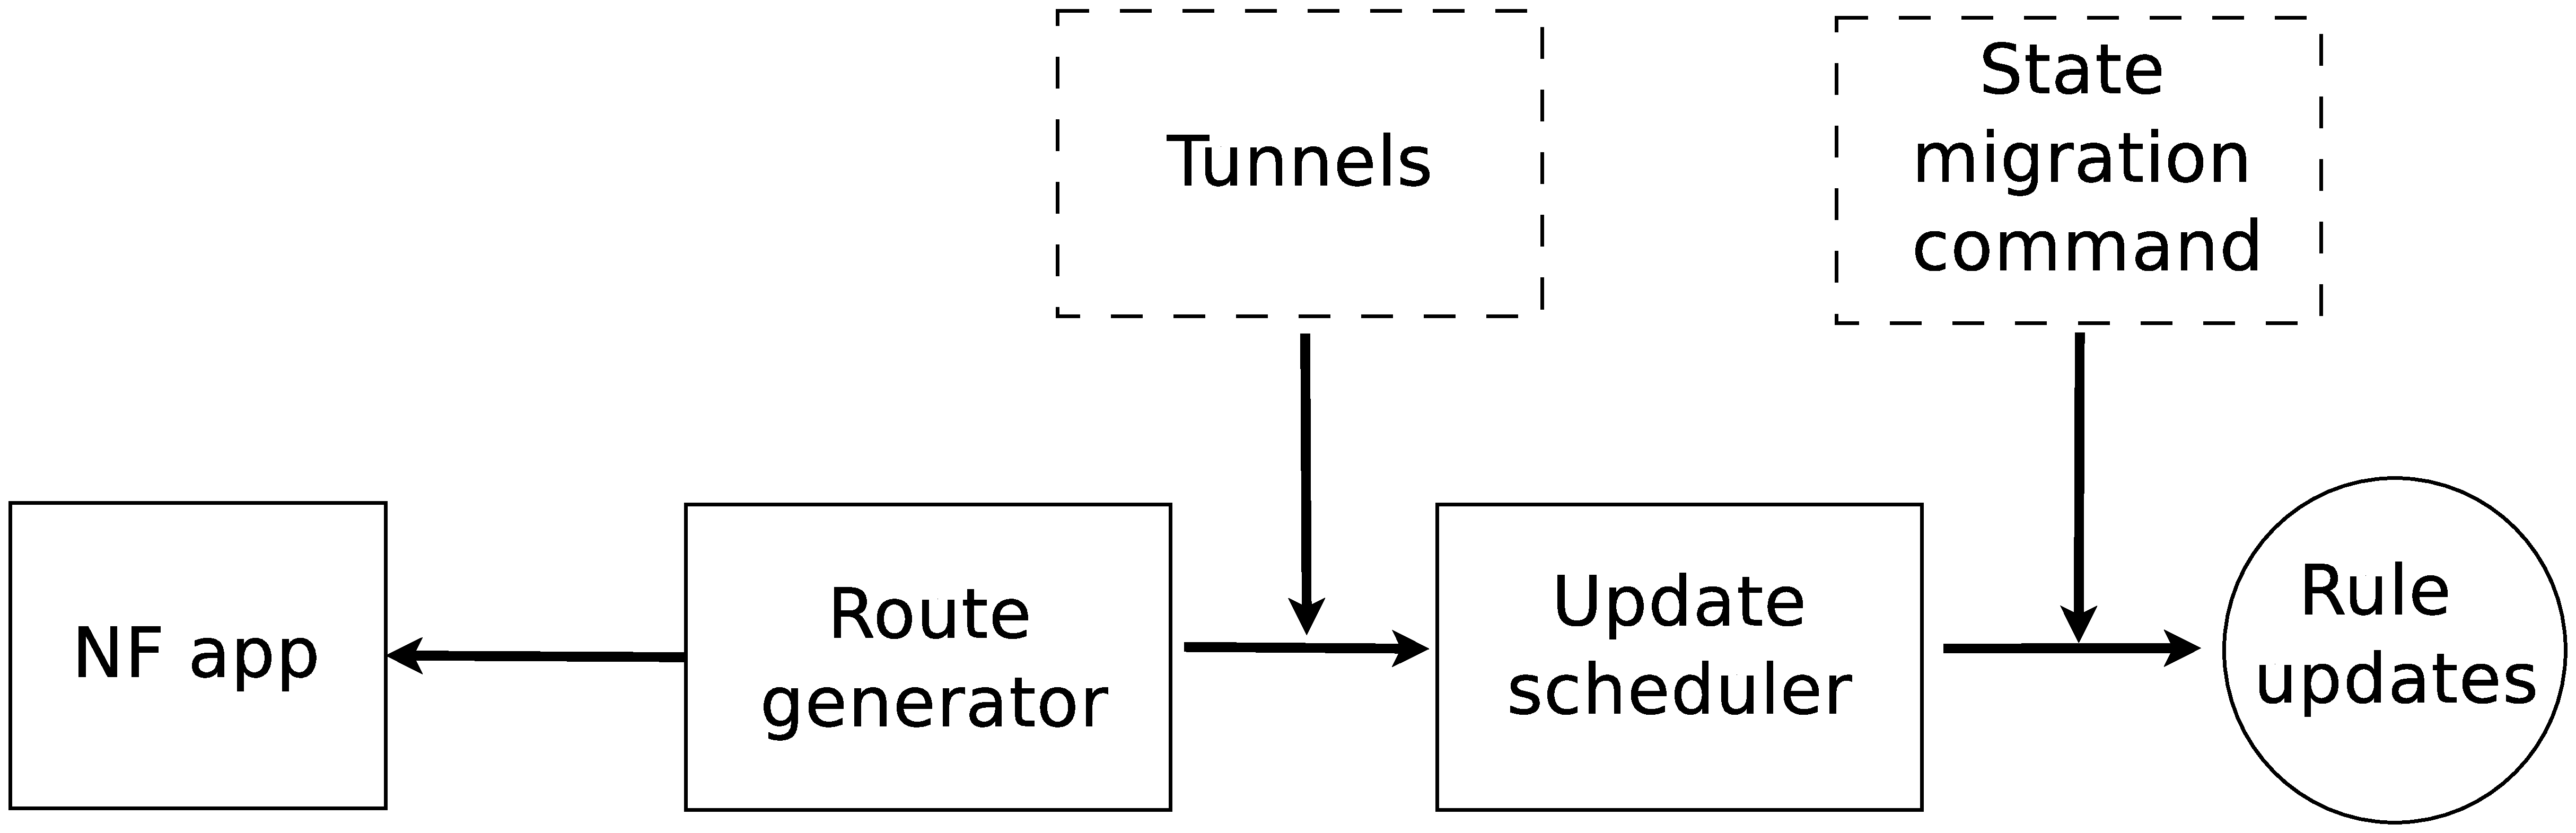
\includegraphics[width=0.9\textwidth]{algorithm.eps}
\caption{Conceptual additions by our algorithm}
\label{fig:algorithm}
\vspace{-0.3cm}
\end{figure}

Our algorithm augments the SDN framework outlined in
\secref{sec:goals} with two conceptual steps (see
\figref{fig:algorithm}).  The first instantiates routing policy for
tunnels to migrate NFs from their old locations to their new locations
and to relocate traffic that arrives at an NF's old location to its
new location.  Once these routes have been determined, the full
routing policy (including these new routes) is then submitted to the
routing-policy update scheduler, which produces the schedule for
deploying rules to switches.  The second phase of our algorithm then
augments this update schedule with commands to bridge traffic on/off
of tunnels as needed, to invoke each NF with packets destined for it
at its new location, and to initiate migration of NFs.  A later phase
of our algorithm (not shown in \figref{fig:algorithm}) cleans up the
bridging rules once they are no longer needed.



The first of these steps is implemented as follows, per \nfID{\nfIdx}
that migrates from \oldSwitchID{\nfIdx} to \newSwitchID{\nfIdx} in
this epoch.

\hspace*{-\parindent}
\fbox{\begin{minipage}[t]{0.95\columnwidth}
\textbf{Migration routes}: The controller constructs a route from
\oldSwitchID{\nfIdx} to \newSwitchID{\nfIdx} to carry flows
\flowIDMigrate{\nfIdx}, \flowIDTunnel{\nfIdx} with source
\oldSwitchID{\nfIdx} and destination \newSwitchID{\nfIdx}.
\flowIDMigrate{\nfIdx}, \flowIDTunnel{\nfIdx} and their associated
route are added to the routing policy that is input to the update
scheduler.
\end{minipage}}

\flowIDMigrate{\nfIdx} will be used to migrate \nfID{\nfIdx} from
\oldSwitchID{\nfIdx} to \newSwitchID{\nfIdx}, and
\flowIDTunnel{\nfIdx} will be used to tunnel packets from
\oldSwitchID{\nfIdx} to \newSwitchID{\nfIdx} that should be processed
by \nfID{\nfIdx}.  Because we assume that the IP addresses of
\oldSwitchID{\nfIdx} and \newSwitchID{\nfIdx} are distinct from the
source and destination addresses of flows routed according to the
policies output from the route generator, the routes chosen to carry
\flowIDMigrate{\nfIdx}, \flowIDTunnel{\nfIdx} cannot contradict the
routes output from the route generator.

\figref{fig:algorithmExample} shows an example for this step.  Suppose
a flow \flowID{} which is processed by \nfID{1} and \nfID{2} needs to
be rerouted from the path $\switchID{1} \rightarrow \switchID{2}
\rightarrow \switchID{3} \rightarrow \switchID{4} \rightarrow
\switchID{5} \rightarrow \switchID{6}$ (solid line) to the path
$\switchID{1} \rightarrow \switchID{7} \rightarrow \switchID{4}
\rightarrow \switchID{8} \rightarrow \switchID{9} \rightarrow
\switchID{6}$ (dash line).  And consequently, the controller decides
to migrate \nfID{1} from \switchID{2} ($= \oldSwitchID{1}$) to
\switchID{7} ($= \newSwitchID{1}$) and \nfID{2} from \switchID{3} ($=
\oldSwitchID{2}$) to \switchID{9} ($= \newSwitchID{2}$).
$\switchID{2} \rightarrow \switchID{1} \rightarrow \switchID{7}$ can
be selected for migration route between \oldSwitchID{1} and
\newSwitchID{1}. $\switchID{3} \rightarrow \switchID{4} \rightarrow
\switchID{8} \rightarrow \switchID{9}$ can be selected for migration
route between \oldSwitchID{2} and \newSwitchID{2}.

\begin{figure}
\centering
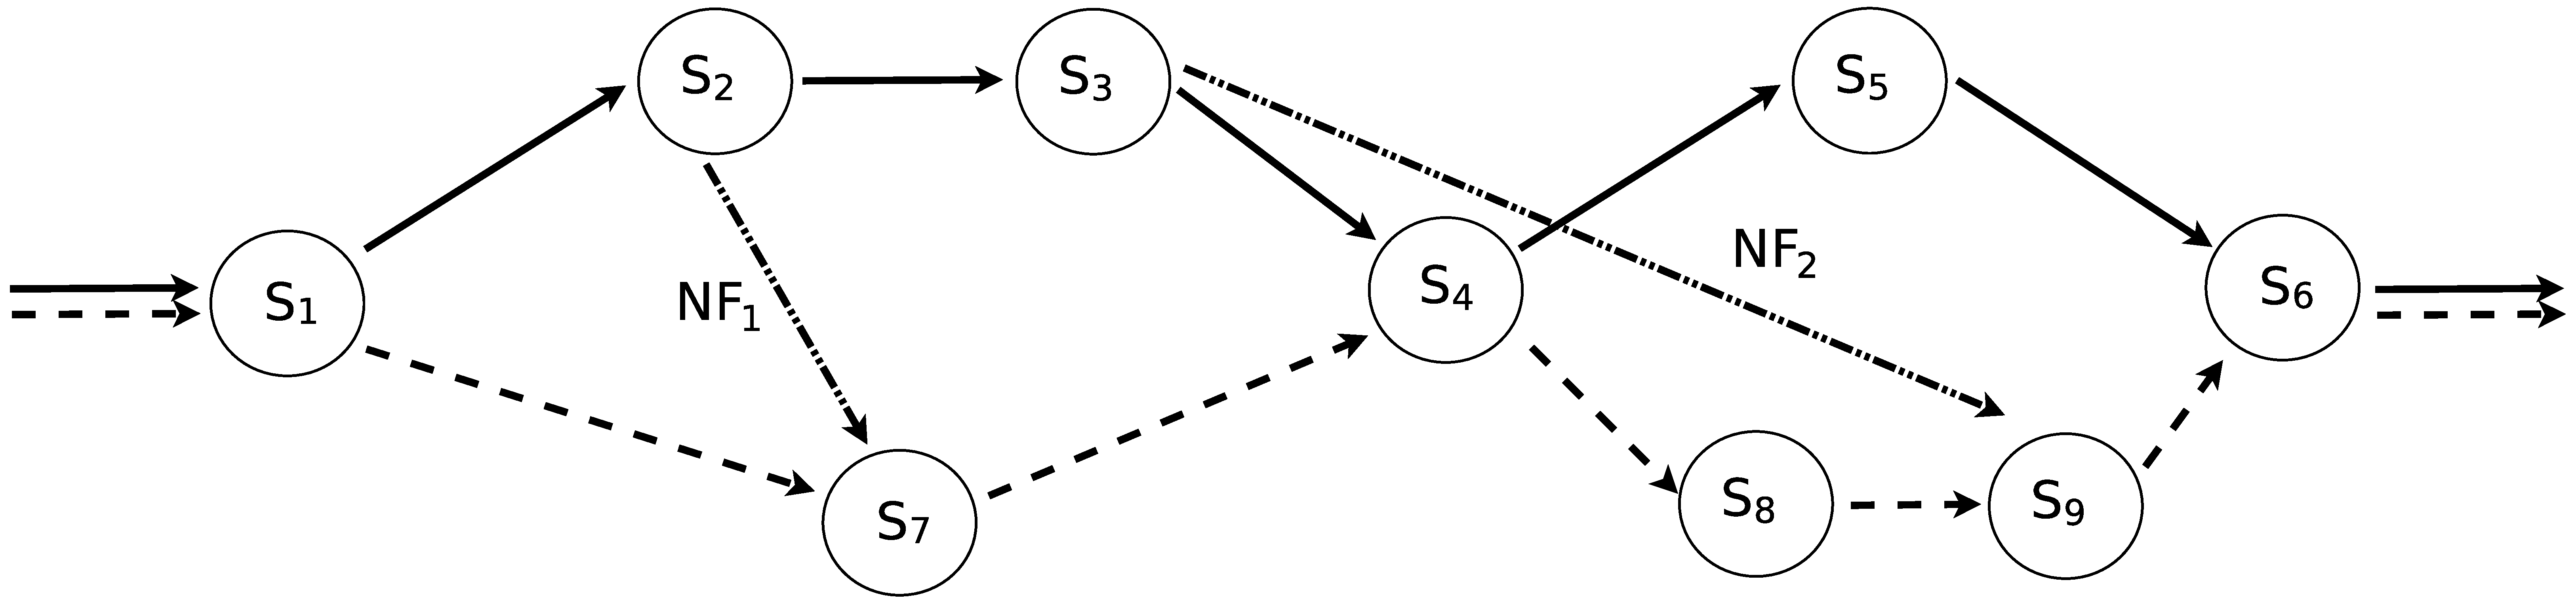
\includegraphics[width=0.95\columnwidth]{algorithmExample.eps}

\caption{Example for algorithm description}
\label{fig:algorithmExample}
\end{figure}

Recall that the update generator now outputs a schedule for rule
deployment in \updateSteps steps $\updateID{1}, \updateID{2}, \ldots,
\updateID{\updateSteps}$, where each \updateID{\updateIdx} includes a
set of \flowAdd and \flowDel commands.  Continuing with the example of
\figref{fig:algorithmExample}, to ensure that packets cannot bypass
waypoints, the update scheduler might formulate the following
three-step schedule.  In the first step, \switchID{7}, \switchID{8},
and \switchID{9} install new rules; i.e., \updateID{1} should include
the flow modification commands for these three switches.  In the
second step (\updateID{2}), \switchID{4} is updated to send packets to
\switchID{8}.  In the third step (\updateID{3}), \switchID{1} is
modified and packets are sent through the new path.  Recall that these
update steps include commands output by the update scheduler to
install rules to route the tunnels generated in the previous step of
our algorithm.

Continuing our algorithm, it first sets $\ruleID{}{\wpField} \gets
\ast$ for any rule \ruleID{} in any \flowAdd or \flowDel command
in any step of the given update schedule $\updateID{1}, \ldots,
\updateID{\updateSteps}$.  Then, for each \nfID{\nfIdx} to be hosted
at a switch \newSwitchID{\nfIdx} in this epoch different from the
switch \oldSwitchID{\nfIdx} where it was hosted in the last, the
controller performs the following steps.

\hspace*{-\parindent} \fbox{\begin{minipage}[t]{0.95\columnwidth}
    \textbf{Rules for routing to \nfID{\nfIdx}}: The controller constructs
    $\wpNmbrMax+2$ rules as follows.  First, the controller constructs
    a rule \ruleIDIn{\nfIdx} with the following fields:
\begin{itemize}[nosep,leftmargin=1em,labelwidth=*,align=left]
  \item $\ruleIDIn{\nfIdx}{\switchField} \gets \oldSwitchID{\nfIdx}$
  \item $\ruleIDIn{\nfIdx}{\coverField} \!\gets\!
    \left\{\flowID{} ~\left|~\!
    \begin{array}{@{}r@{\hspace{0.25em}}r@{}}
      \exists \pktID{}, \ruleID{}: & \pktID{} \in \flowID{} \\
      \wedge & \ruleID{} \in \oldSwitchID{\nfIdx}{\ruleSet} \\
      \wedge & \ruleID{} = \ruleMatchNew{\oldSwitchID{\nfIdx}}{\pktID{}}\\
      \wedge & \ruleID{}{\sendToField} = \nfID{\nfIdx}
    \end{array}
    \right.
    \right\}$
  \item $\ruleIDIn{\nfIdx}{\wpField} \gets \ast$
  \item $\ruleIDIn{\nfIdx}{\priorityField} \gets \infty$
  \item $\ruleIDIn{\nfIdx}{\sendToField} \gets
    \encapsulate{\flowIDTunnel{\nfIdx}}$
\end{itemize}
In addition, the controller constructs the rule \ruleIDOut{} with
the following fields:
\begin{itemize}[nosep,leftmargin=1em,labelwidth=*,align=left]
  \item $\ruleIDOut{\nfIdx}{\switchField} \gets \newSwitchID{\nfIdx}$
  \item $\ruleIDOut{\nfIdx}{\coverField} \gets \{\flowIDTunnel{\nfIdx}\}$
  \item $\ruleIDOut{\nfIdx}{\wpField} \gets \ast$
  \item $\ruleIDOut{\nfIdx}{\priorityField} \gets \infty$
  \item $\ruleIDOut{\nfIdx}{\sendToField} \gets \decapsulate$
\end{itemize}
Finally, for each $\wpIdx \in \nats{\wpNmbrMax}$, the controller
constructs a rule \ruleIDInv{\nfIdx}{\wpIdx} with the following
fields:
\begin{itemize}[nosep,leftmargin=1em,labelwidth=*,align=left]
  \item $\ruleIDInv{\nfIdx}{\wpIdx}{\switchField} \gets \newSwitchID{\nfIdx}$
  \item $\ruleIDInv{\nfIdx}{\wpIdx}{\coverField} \gets \{\flowID{} \mid \wpFn{\flowID{}}{\wpIdx} = \nfIdx\}$
  \item $\ruleIDInv{\nfIdx}{\wpIdx}{\wpField} \gets \wpIdx$
  \item $\ruleIDInv{\nfIdx}{\wpIdx}{\priorityField} \gets \infty$
  \item $\ruleIDInv{\nfIdx}{\wpIdx}{\sendToField} \gets \nfID{\nfIdx}$
\end{itemize}
\end{minipage}}

In the example of \figref{fig:algorithmExample}, \switchID{2} and
\switchID{3} should install rule \ruleIDIn{1} and \ruleIDIn{2},
respectively, to encapsulate packets of \flowID{} onto
\flowIDTunnel{\nfIdx}.  In this way, packets arriving at \switchID{2}
or \switchID{3} can be relocated to new positions \switchID{7} and
\switchID{9}, respectively, during NF migration. Packets relocated
through these tunnels to the new NF locations should be decapsulated
back to the original flow \flowID{} such that they can traverse the
remainder of the new path after being processed by the appropriate
NF. Therefore, \switchID{7} and \switchID{9} need rules \ruleIDOut{1}
and \ruleIDOut{2}, respectively.

\ruleIDInv{\nfIdx}{\wpIdx} has two functions. First, it sends packets
that need to be processed (i.e., with waypoint counter \wpIdx where
$\wpFn{\flowID{}}(\wpIdx) = \nfIdx$) to \nfID{\nfIdx}.  Note that
packets on \flowID{} output from \nfID{\nfIdx} will have a waypoint
counter of $\wpIdx+1$ and thus will not be matched to
\ruleIDInv{\nfIdx}{\wpIdx} again.  Second, \ruleIDInv{\nfIdx}{\wpIdx}
prevents packets from being processed twice by \nfID{\nfIdx}.
Continuing with the example of \figref{fig:algorithmExample}, since at
the beginning of $\updateID{3}$, \switchID{4} has been updated (in
\updateID{2}) but \switchID{1} has not yet been changed, packets on
\flowID{} traversing a part of old path ($\switchID{1} \rightarrow
\switchID{2} \rightarrow \switchID{3} \rightarrow \switchID{4}$) and a
part of new path ($\switchID{4} \rightarrow \switchID{8} \rightarrow
\switchID{9} \rightarrow \switchID{6}$) encounter both the old
(\switchID{3}) and new position (\switchID{9}) of \nfID{2}.
$\ruleIDInv{2}{2}$ at \switchID{9} ensures packets carrying waypoint
counter $2$ can be processed by \nfID{2}, but packets with waypoint
counter $3$ (\nfID{2} already processed these packets at \switchID{3})
are forwarded to next switch \switchID{6} immediately.

Now that these rules have been generated, we need to integrate them
into the update schedule.  To do so, the algorithm initializes
\updateID{\updateSteps+1} to be empty, i.e.,
$\updateID{\updateSteps+1} \gets \{\}$.  Then, for each migrating
network function \nfID{\nfIdx}, the controller performs the following.

\hspace*{-\parindent}
\fbox{\begin{minipage}[t]{0.95\columnwidth}
\textbf{Update schedule}: To deploy \ruleIDIn{\nfIdx},
\ruleIDOut{\nfIdx}, $\{\ruleIDInv{\nfIdx}{\wpIdx}\}_{\wpIdx \in
  \nats{\wpNmbrMax}}$ in the update schedule \updateID{1},
\updateID{2}, $\ldots$, \updateID{\updateSteps+1}, the controller
performs the following steps.
\begin{itemize}[nosep,leftmargin=1em,labelwidth=*,align=left]
  \item The controller adds
    \newSwitchID{\nfIdx}{\flowAdd{\ruleIDOut{\nfIdx}}},
    \newSwitchID{\nfIdx}{\import{\nfIdx}{\switchIdx}}, and
    \newSwitchID{\nfIdx}{\flowAdd{\ruleIDInv{\nfIdx}{\wpIdx}}} for
    each $\wpIdx \in \nats{\wpNmbrMax}$ to \updateID{1},
    where $\oldSwitchID{\nfIdx} = \switchID{\switchIdx}$.
  \item The controller searches for the last step
    \updateID{\updateIdx} in which rules to route
    \flowIDMigrate{\nfIdx}, \flowIDTunnel{\nfIdx} are deployed.  It
    adds \oldSwitchID{\nfIdx}{\flowAdd{\ruleIDIn{\nfIdx}}} and
    \oldSwitchID{\nfIdx}{\export{\nfIdx}{\switchIdx}} to
    \updateID{\updateIdx+1} where $\newSwitchID{\nfIdx} =
    \switchID{\switchIdx}$.
  \item The controller adds \newSwitchID{\nfIdx}{\release{\nfIdx}} to
    \updateID{\updateSteps+1}.
  \end{itemize}
\end{minipage}}

The first bullet incorporates commands to prepare switches at new
positions for NF migration. 
In the example of \figref{fig:algorithmExample}, the controller issues commands \switchID{7}{\import{1}{2}}, \switchID{7}{\flowAdd{\ruleIDOut{1}}} and \switchID{7}{\flowAdd{\ruleIDInv{1}{1}}} to \switchID{7}. So \switchID{7} waits for messages from \switchID{2} and prepares to reconstruct \nfID{1} locally. The controller also performs similar operations on \switchID{9}.

The second bullet incorporates commands to migrate \nfID{\nfIdx} from its old to its new
position. This should be done after the rules implementing the
migration route have been deployed (i.e., after step
$\updateID{\updateIdx}$). 
In the example of \figref{fig:algorithmExample}, assume the controller deploys rules to create a tunnel $\switchID{2} \rightarrow \switchID{1} \rightarrow \switchID{7}$ to migrate \nfID{1} from \switchID{2} to \switchID{7} in step \updateID{1}. Then, in step \updateID{2}, the controller can use the interface \switchID{2}{\export{1}{7}} to instruct \switchID{2} to create a set of packets to marshal \nfID{1} and send these packets to \switchID{7}. Upon receiving packets from \switchID{2}, \switchID{7} reconstructs \nfID{1} and starts to perform \nfID{1}{}{\processPkt} invocations. Meanwhile, \switchID{2} uses the rule \ruleIDIn{1} to encapsulate the packets of \flowID{} to packets of \flowIDTunnel{1}. Packets of \flowIDTunnel{1} are then forwarded to \switchID{7} and \switchID{7} uses the rule \ruleIDOut{1} to decapsulate these packets back to packets of \flowID{}. The packets have not been processed by \switchID{2} and therefore should carry the waypoint counter $1$. Thus, \switchID{7} uses the rule \ruleIDInv{1}{1} to forward packets to \nfID{1}. After processed by \nfID{1}, these packets are buffered at \switchID{7} with the waypoint counter $2$.

The last bullet ensures that packets
released from switches at new positions can be matched to rules
implementing new routing policy at all downstream switches.
In the example of \figref{fig:algorithmExample}, the controller sends \switchID{7}{\release{1}} in step \updateID{4}. \switchID{7} then releases the buffered packets to the network since \switchID{4}, \switchID{8} and \switchID{9} have installed rules to forward packets to the destination.

The last step of our algorithm cleans up migration-related rules once
they will no longer be used.  Specifically, for each migrated
\nfID{\nfIdx}, the following is performed:

\hspace*{-\parindent}
\fbox{\begin{minipage}[t]{0.95\columnwidth}
\textbf{Bridging rules cleanup}: After sufficient time passes to
ensure that \flowIDMigrate{\nfIdx} and \flowIDTunnel{\nfIdx} will
contain no more packets, the controller issues
\oldSwitchID{\nfIdx}{\flowDel{\ruleIDIn{\nfIdx}}} and
\newSwitchID{\nfIdx}{\flowDel{\ruleIDOut{\nfIdx}}} commands.
\end{minipage}}

In \figref{fig:algorithmExample}, this step causes the deletion of
\ruleIDIn{1} and \ruleIDOut{1} from \switchID{2} and \switchID{7},
respectively, and the deletion of \ruleIDIn{2} and \ruleIDOut{2} from
\switchID{3} and \switchID{9}, respectively.  The rules to implement
the migration routes $\switchID{2} \rightarrow \switchID{1}
\rightarrow \switchID{7}$ and $\switchID{3} \rightarrow \switchID{4}
\rightarrow \switchID{8} \rightarrow \switchID{9}$ can also be
removed, if doing so does not disrupt other routing policy.

\section{Update Scheduling}
\label{sec:schedule}

The algorithm described in the previous section adapts a given update
schedule with additional \flowDel, \flowAdd, \export, \import, and
\release commands to migrate NFs during path updates.  In this
section, we explore the requirements for the given update schedule
that, when combined with the algorithm of the previous section,
ensures waypoint correctness as defined in
\secref{sec:goals:correctness}.  We define a sufficient condition in
\secref{sec:schedule:condition}.  Finally, in
\secref{sec:schedule:rwc} we provide an update scheduling algorithm
that is tailored to implement specifically this condition.

\subsection{A Sufficient Condition for Waypoint Correctness}
\label{sec:schedule:condition}

In this section we give a sufficient condition for the NF-migration
algorithm of \secref{sec:migration} to ensure the waypoint correctness
property defined in \secref{sec:goals:correctness}.  Recall that
during a route change, each \nfID{\nfIdx} is migrated from its old
location \oldSwitchID{\nfIdx} to its new location
\newSwitchID{\nfIdx}, while traffic to be processed by \nfID{\nfIdx}
that arrives at \oldSwitchID{\nfIdx} and matched to a rule \ruleID{}
with $\ruleID{}{\sendToField} = \nfID{\nfIdx}$ is transported from
\oldSwitchID{\nfIdx} to \newSwitchID{\nfIdx} to be processed once
\nfID{\nfIdx} is reconstituted there.  Whether traffic reaches
\newSwitchID{\nfIdx} via this mechanism or by the new routing policy
does not matter.  Rather, all that really matters is that a packet on
flow \flowID{} with waypoint counter \wpIdx reaches either
\oldSwitchID{\wpFn{\flowID{}}{\wpIdx}} or
\newSwitchID{\wpFn{\flowID{}}{\wpIdx}}.  We call this property
\textit{relaxed waypoint correctness}:

\paragraph{Relaxed waypoint correctness} An update scheduling algorithm
satisfies \textit{relaxed waypoint correctness} if during any route
update, it ensures that for each flow \flowID{} and each $\wpIdx \in
\nats{\wpNmbr{\flowID{}}}$, each packet on flow \flowID{} with
waypoint counter \wpIdx reaches \oldSwitchID{\wpFn{\flowID{}}{\wpIdx}}
or \newSwitchID{\wpFn{\flowID{}}(\wpIdx)}.\footnote{Strictly speaking,
  since a packet on flow \flowID{} has its waypoint counter
  incremented to $\wpIdx+1$ right \textit{before} processing by
  \nfID{\nfIdx} for $\nfIdx = \wpFn{\flowID{}}(\wpIdx)$, it is
  possible that this property will fail for a packet that is not then
  output from \nfID{\nfIdx} (e.g., because \nfID{\nfIdx} drops it).
  We require this property for every packet on \flowID{} output from
  \nfID{\nfIdx}, however.}

\medskip

Our NF-migration algorithm in \secref{sec:migration} guarantees the waypoint correctness property defined in \secref{sec:goals:correctness}, if the underlying update scheduling algorithm (used by the update scheduler in the controller) satisfies the relaxed waypoint correctness.
An example of an update scheduling algorithm that implements this
property is CU~\cite{CU}, which on its own ensures that each packet
traverses either the old path in its entirety or the new path in its
entirety.  When conjoined with our NF migration algorithm, a packet
that is being routed along its old path might be tunneled from
\oldSwitchID{\nfIdx} to \newSwitchID{\nfIdx} for processing by
\nfID{\nfIdx}, after which it will be buffered until the route update
is complete.  From that point forward, it will be routed along its new
path.  A natural question is whether there are route update algorithms
that satisfy relaxed waypoint correctness without enforcing a packet
to traverse only the path of its old flow or of its new one.  In
the next section we answer this question in the affirmative.

%\input{modelchecking}


\subsection{Update Scheduling for Relaxed Waypoint Correctness}
\label{sec:schedule:rwc}

In this section we provide an update scheduling algorithm, which we
call \ourRouteUpdateName (for \ourRouteUpdateNameLong), that is
specifically designed to satisfy relaxed waypoint correctness, no
more, no less, whenever it is possible to achieve this property while
updating each switch only once during an epoch change.  The algorithm
is inspired by the TSU~\cite{tsu} routing update algorithm, though we
have adapted it to accommodate NF migration and waypoint ordering.

The algorithm computes the update schedule \updateID{1}, \updateID{2},
$\ldots$, \updateID{\updateSteps} using an optimization expressed as a
0-1 integer linear program, which can be solved (if it has a solution)
using solvers like CPLEX~\cite{CPLEX} or Gurobi~\cite{gurobi}.  This algorithm assumes that the
old and new routing policies differ only in a single path; i.e., a
flow \flowID{} (or set of flows) transitions from the same old path to
the same new path.  (Multiple path changes can be implemented
one-by-one in multiple updates.)  Moreover, this algorithm assumes
that both the old and new path are loop-free.

\subsubsection{Integer program}
\label{sec:schedule:tsu:ip}

Let \oldSwitchesSet be the set of switches that appear on the old
path; \newSwitchesSet the set of switches that appear on the new path;
$\switchesSet = \oldSwitchesSet \cup \newSwitchesSet$; $\oldPathNB{}
\subseteq \oldSwitchesSet \times \oldSwitchesSet$ the links comprising
the old path; and $\newPathNB{} \subseteq \newSwitchesSet \times
\newSwitchesSet$ the links comprising the new path.  Therefore,
$\oldPathNB{} \setminus \newPathNB{}$ is the set of links that will be
\textit{disabled} by the path change (i.e., that will no longer be
traversed by the rerouted flow \flowID{}), and $\newPathNB{} \setminus
\oldPathNB{}$ is the set of links that will be \textit{enabled} by the
path change.  Let $\switchesWLinkSwapSet \subseteq \oldSwitchesSet
\cap \newSwitchesSet$ contain the switches at which links to carry
\flowID{} must be both enabled and disabled, i.e.,
$\switchID{\switchIdx} \in \switchesWLinkSwapSet$ iff
$\switchID{\switchIdx} \in \oldSwitchesSet \cap \newSwitchesSet$ and
for some \switchID{\switchIdxAlt}, $(\switchID{\switchIdx},
\switchID{\switchIdxAlt}) \in (\oldPathNB{} \setminus \newPathNB{}) \cup
(\newPathNB{} \setminus \oldPathNB{})$.  Let \enableLinksSet be the new links
enabled at the switches in \switchesWLinkSwapSet, and let
\disableLinksSet bet the old links disabled at the switches in
\switchesWLinkSwapSet; i.e., $(\switchID{\switchIdx},
\switchID{\switchIdxAlt}) \in \enableLinksSet$ iff
$\switchID{\switchIdx} \in \switchesWLinkSwapSet$ and
$(\switchID{\switchIdx}, \switchID{\switchIdxAlt}) \in \newPathNB{}
\setminus \oldPathNB{}$, and $(\switchID{\switchIdx},
\switchID{\switchIdxAlt}) \in \disableLinksSet$ iff
$\switchID{\switchIdx} \in \switchesWLinkSwapSet$ and
$(\switchID{\switchIdx}, \switchID{\switchIdxAlt}) \in \oldPathNB{}
\setminus \newPathNB{}$.  For a natural number \genericNat, let
$\nats{\genericNat} = \{1, \ldots, \genericNat\}$.


\begin{figure*}[t]
\centering
\noindent
\fbox{\begin{minipage}{0.95\linewidth}
  
  \begin{align}
    \mathclap{\mbox{Minimize } \updateStepsAlt \mbox{ subject to:}}
    \label{eqn:update:goal} \\
    \updateStepsAlt & \geq \updateIdx \cdot \switchUpdateInd{\updateIdx}{\switchIdx}
    & \forall \updateIdx \in \nats{\switchNmbr}, \switchID{\switchIdx} \in \switchesWLinkSwapSet
    \label{eqn:update:roundBound} \\
    1 & = \sum_{\updateIdx \in \nats{\switchNmbr}} \switchUpdateInd{\updateIdx}{\switchIdx}
    & \forall \switchID{\switchIdx} \in \switchesWLinkSwapSet
    \label{eqn:update:oneChange} \\
    \linkActiveInd{\updateIdx}{\switchIdx}{\switchIdxAlt} & = 1 - \sum_{\updateIdxAlt \leq \updateIdx} \switchUpdateInd{\updateIdxAlt}{\switchIdx}
    & \forall \updateIdx \in \nats{\switchNmbr}, (\switchID{\switchIdx}, \switchID{\switchIdxAlt}) \in \disableLinksSet
    \label{eqn:update:disableLinks} \\
    \linkActiveInd{\updateIdx}{\switchIdx}{\switchIdxAlt} & = \sum_{\updateIdxAlt \leq \updateIdx} \switchUpdateInd{\updateIdxAlt}{\switchIdx}
    & \forall \updateIdx \in \nats{\switchNmbr}, (\switchID{\switchIdx}, \switchID{\switchIdxAlt}) \in \enableLinksSet
    \label{eqn:update:enableLinks} \\
    \linkActiveInd{\updateIdx}{\switchIdx}{\switchIdxAlt} & = 1
    & \forall \updateIdx \in \nats{\switchNmbr},
    (\switchID{\switchIdx}, \switchID{\switchIdxAlt}) \in
    (\oldPathNB{} \cup \newPathNB) \setminus (\enableLinksSet \cup \disableLinksSet)
    \label{eqn:update:keepLinks} \\
    \todoNF{\updateIdx}{\wpIdx}{\switchIdxAlt} & \geq \todoNF{\updateIdx}{\wpIdx}{\switchIdx} + \linkActiveInd{\updateIdx-1}{\switchIdx}{\switchIdxAlt} - 1
    & \forall \updateIdx \in \nats{\switchNmbr}, \wpIdx \in \nats{\wpNmbr{\flowID{}}}, \switchID{\switchIdxAlt} \in \switchesSet,
     \switchID{\switchIdx} \in \switchesSet \setminus \{\oldSwitchID{\wpFn{\flowID{}}{\wpIdx}}, \newSwitchID{\wpFn{\flowID{}}{\wpIdx}}\}
    \label{eqn:update:stillToDoBegin} \\
    \todoNF{\updateIdx}{\wpIdx}{\switchIdxAlt} & \geq \todoNF{\updateIdx}{\wpIdx}{\switchIdx} + \linkActiveInd{\updateIdx}{\switchIdx}{\switchIdxAlt} - 1
    & \forall \updateIdx \in \nats{\switchNmbr}, \wpIdx \in \nats{\wpNmbr{\flowID{}}}, \switchID{\switchIdxAlt} \in \switchesSet,
     \switchID{\switchIdx} \in \switchesSet \setminus \{\oldSwitchID{\wpFn{\flowID{}}{\wpIdx}}, \newSwitchID{\wpFn{\flowID{}}{\wpIdx}}\}
    \label{eqn:update:stillToDoEnd} \\
    \todoNF{\updateIdx}{\wpIdx}{\switchIdx} & = 1
    & \forall \updateIdx \in \nats{\switchNmbr}, \wpIdx \in \nats{\wpNmbr{\flowID{}}}, \switchID{\switchIdx} \in \{\inSwitch{\flowID{}}\}
    \label{eqn:update:toDo} \\
    \todoNF{\updateIdx}{\wpIdx}{\switchIdx} & = 0
    & \forall \updateIdx \in \nats{\switchNmbr}, \wpIdx \in \nats{\wpNmbr{\flowID{}}}, \switchID{\switchIdx} \in \{\outSwitch{\flowID{}}\}
    \label{eqn:update:done} \\
    \todoNF{\updateIdx}{\wpIdx+1}{\switchIdx} & \ge \todoNF{\updateIdx}{\wpIdx}{\switchIdx}
    & \forall \updateIdx \in \nats{\switchNmbr}, \wpIdx \in \nats{\wpNmbr{\flowID{}}-1},
    \switchID{\switchIdx} \in \switchesSet
    \label{eqn:update:order}
  \end{align}
\end{minipage}}
\caption{\ourRouteUpdateName integer program for generating update schedule \label{fig:update}}
\end{figure*}


The optimization, shown in \figref{fig:update}, minimizes the number
\updateStepsAlt of update steps subject to constraints
\eqnrefs{eqn:update:roundBound}{eqn:update:order}.
\switchUpdateInd{\updateIdx}{\switchIdx} is a binary indicator
variable signaling whether switch $\switchID{\switchIdx} \in
\switchesWLinkSwapSet$ is updated in step \updateIdx; i.e., if the
solution to the integer program has
$\switchUpdateInd{\updateIdx}{\switchIdx} = 1$, then the controller
will include its updates to \switchID{\switchIdx} in
\updateID{\updateIdx}.  Constraint~\eqnref{eqn:update:oneChange}
ensures that each switch in \switchesWLinkSwapSet is updated exactly
once.

The binary variable
\linkActiveInd{\updateIdx}{\switchIdx}{\switchIdxAlt} for each
$(\switchID{\switchIdx}, \switchID{\switchIdxAlt}) \in \oldPathNB{} \cup
\newPathNB{}$ indicates whether the rerouted flows will be forwarded
directly from \switchID{\switchIdx} to \switchID{\switchIdxAlt} as of
the end of update \updateID{\updateIdx}.
Constraint~\eqnref{eqn:update:disableLinks} ensures that
$\linkActiveInd{\updateIdx}{\switchIdx}{\switchIdxAlt} = 0$ once link
$(\switchID{\switchIdx}, \switchID{\switchIdxAlt}) \in
\disableLinksSet$ has been disabled, and
constraint~\eqnref{eqn:update:enableLinks} ensures that
$\linkActiveInd{\updateIdx}{\switchIdx}{\switchIdxAlt} = 1$ once link
$(\switchID{\switchIdx}, \switchID{\switchIdxAlt}) \in
\enableLinksSet$ has been enabled.
Constraint~\eqnref{eqn:update:keepLinks} ensures that
$\linkActiveInd{\updateIdx}{\switchIdx}{\switchIdxAlt} = 1$ for any
other link in $\oldPathNB{} \cup \newPathNB{}$.

The binary variable \todoNF{\updateIdx}{\wpIdx}{\switchIdx} indicates
whether a packet on the rerouted flow \flowID{}, upon reaching switch
\switchIdx after the end of update $\updateIdx-1$ and before the end
of update \updateIdx, has yet to be processed by \nfID{\nfIdx} where
$\nfIdx = \wpFn{\flowID{}}{\wpIdx}$.
Constraints~\eqnref{eqn:update:stillToDoBegin}
and~\eqnref{eqn:update:stillToDoEnd} ensure that if
$\linkActiveInd{\updateIdx-1}{\switchIdx}{\switchIdxAlt} =
\linkActiveInd{\updateIdx}{\switchIdx}{\switchIdxAlt} = 1$ and so the
packet is forwarded directly from \switchID{\switchIdx} to
\switchID{\switchIdxAlt}, and if the packet was not yet processed by
\nfID{\nfIdx} upon reaching \switchID{\switchIdx} (i.e.,
$\todoNF{\updateIdx}{\wpIdx}{\switchIdx} = 1$), then it still remains
to be processed upon reaching \switchID{\switchIdxAlt} (i.e.,
$\todoNF{\updateIdx}{\wpIdx}{\switchIdxAlt} = 1$).  Of course, this
reasoning is valid only if $\switchID{\switchIdx} \not\in
\{\oldSwitchID{\nfIdx}, \newSwitchID{\nfIdx}\}$; if
$\switchID{\switchIdx} = \oldSwitchID{\nfIdx}$ then the packet will be
processed by \nfID{\nfIdx} there, and if $\switchID{\switchIdx} =
\newSwitchID{\nfIdx}$ then the packet will be buffered at
\switchID{\switchIdx} awaiting \nfID{\nfIdx}.  Therefore,
constraints~\eqnref{eqn:update:stillToDoBegin}
and~\eqnref{eqn:update:stillToDoEnd} are included only for
$\switchID{\switchIdx} \not\in \{\oldSwitchID{\nfIdx},
\newSwitchID{\nfIdx}\}$.  Constraints~\eqnref{eqn:update:toDo}
and~\eqnref{eqn:update:done} indicate that the packets on flow
\flowID{} have yet to be processed by \nfID{\nfIdx} upon their arrival
at their ingress \inSwitch{\flowID{}} and must be processed by
\nfID{\nfIdx} upon departing the network at their egress
\outSwitch{\flowID{}}.  Finally, constraint~\eqnref{eqn:update:order}
ensures that if a packet has yet to be processed by \nfID{\nfIdx} for
$\nfIdx = \wpFn{\flowID{}}{\wpIdx}$, then it also has yet to be
processed by \nfID{\nfIdxAlt} for $\nfIdxAlt =
\wpFn{\flowID{}}{\wpIdx+1}$.

\subsubsection{Generating the update schedule}
\label{sec:schedule:tsu:schedule}

Given a solution to the integer program of \figref{fig:update}, the
update scheduler generates the update schedule as follows.  We assume
that $\switchesSet \setminus ((\oldSwitchesSet \cap \newSwitchesSet)
\setminus \switchesWLinkSwapSet)$ is the set of switches at which the
new rules \newRules to implement the new routing policy differ from
the rules \oldRules already deployed to the network to implement the
old routing policy.
\begin{itemize}[nosep,leftmargin=1em,labelwidth=*,align=left]
\item For each $\switchID{\switchIdx} \in \newSwitchesSet
  \setminus \oldSwitchesSet$, the update scheduler adds
  \switchID{\switchIdx}{\flowAdd{\ruleID{}}} to \updateID{1} for each
  $\ruleID{} \in \newRules\setminus\oldRules$ for which
  $\ruleID{}{\switchField} = \switchID{\switchIdx}$.

\item For $\switchID{\switchIdx} \in \switchesWLinkSwapSet$ for
  which $\switchUpdateInd{\updateIdx}{\switchIdx} = 1$, the update
  scheduler adds \switchID{\switchIdx}{\flowAdd{\ruleID{}}} to
  \updateID{\updateIdx+1} for each $\ruleID{} \in
  \newRules\setminus\oldRules$ for which $\ruleID{}{\switchField} =
  \switchID{\switchIdx}$, and \switchID{}{\flowDel{\ruleID{}}} to
  \updateID{\updateIdx+1} for each $\ruleID{} \in
  \oldRules\setminus\newRules$ for which $\ruleID{}{\switchField} =
  \switchID{\switchIdx}$.

\item For $\switchID{\switchIdx} \in \oldSwitchesSet \setminus
  \newSwitchesSet$, the scheduler adds
  \switchID{\switchIdx}{\flowDel{\ruleID{}}} to \updateID{\updateStepsAlt+2} and for each $\ruleID{} \in \oldRules\setminus\newRules$ for
  which $\ruleID{}{\switchField} = \switchID{\switchIdx}$.
\end{itemize}
After we obtain the update schedule \updateID{1}, \updateID{2},
$\ldots$, \updateID{\updateSteps} ($\updateSteps = \updateStepsAlt + 2$), it can then be turned over to the algorithm of
\secref{sec:migration:algo} for adaptation as prescribed there.


\section{Implementation}
\label{sec:implementation}

We implemented our NF migration algorithm (\secref{sec:migration})
using Open vSwitch~\cite{ovs} and the Ryu
controller~\cite{ryu}. Packets' waypoint counters were stored in six
bits of the VLAN tag, permitting up to $\wpNmbrMax = 2^6 - 2$
waypoints per flow.  PRADS~\cite{prads} was used to instantiate
network functions and was modified to provide APIs for migration. We
used and implemented three underlying route-update algorithms, namely
SCC, CU~\cite{CU}, and \ourRouteUpdateName to generate
rule-deployment schedules to transition to a new routing policy. We
incorporated our state migration algorithm into the rule-update
schedule as described in \secref{sec:migration} to achieve waypoint
correctness.  The \ourRouteUpdateName integer program in
\figref{fig:update} was solved using Gurobi~\cite{gurobi}.

\subsection{Route-Update Algorithms}
\label{sec:implementation:route}

\paragraph{SCC}
\iffalse
SCC is a route-update algorithm that uses rule timestamps and packet
timestamps to ensure a property the authors call \textit{suffix causal
  consistency}.  In SCC, each packet carries a packet
timestamp that may be changed by the rules to which it is matched as
it traverses switches in the network. Each switch receiving this
packet searches for the rule of the highest priority in its flow table
that covers this packet and ensures this rule is recent enough to
match to this packet by comparing the packet timestamp with the rule
timestamp.  To implement relaxed waypoint correctness, the algorithm
performs updates in two steps. First, the ingress switch is updated to
guarantee packets can be matched to rules consistent with the new
routing policy.  Then the remaining switches are updated
simultaneously to forward each packet through its new path.
\fi

We optimized the implementation of our SCC algorithm described in \chapref{chap:scc}.
Our implementation leverages unused header bits, namely six bits of
the VLAN tag, to store the timestamp in each packet.  (The remaining
six bits of the VLAN tag was used to record the packet's waypoint
counter, as already mentioned.)  We
modified Open vSwitch(OVS) to extract these bits from each packet and
to set these bits based on the action of the rule to which it is
matched. The SCC rule timestamp value for each rule \ruleID{} is
embedded into the corresponding field of the rule to avoid changing
the OpenFlow protocol used between OVS and the controller. However,
this value is not used for rule matching.  Rather, it is extracted
from the rule upon rule installation and masked during matching. If
the timestamp of the rule to which the packet is matched is smaller
than the packet timestamp, then this packet is buffered awaiting
more up-to-date rules.

Since OVS does not provide packet buffering anymore, we connected each
OVS with a local Ryu controller. Instead of buffering packets itself,
OVS forwards packets to the local controller. The local controller
is in charge of buffering packets and updating rules for this
switch. A globally centralized controller running our algorithm uses a
RESTful API to issue rule modification commands to the local
controller. Then the local controller updates OVS using OpenFlow and
also sends buffered packets back to the switch when appropriate.


\paragraph{CU}
\iffalse
Consistent Update (CU) uses a two-phase commit to apply rule updates
atomically throughout a network.  Like SCC, each ingress switch marks
each inbound packet with a timestamp indicating if the old or new
configuration should be used to route it, and each downstream switch
uses rules with the same timestamp to match the packet. However,
unlike SCC, the timestamp carried by the packet will not be changed as
it traverses the network. The algorithm first deploys, but does not
yet enable, rules with a new timestamp at all switches.  Then, after
all the new rules have been installed, the controller updates the
ingress switch to start tagging packets with the new timestamp to
allow each downstream switch to apply the new
configuration. Therefore, CU makes each packet traverse either its old
or new path in its entirety, and in this way enforces relaxed waypoint
correctness. After waiting sufficient time for any packets marked with
the old timestamp to have departed the network, the controller
instructs all switches to delete the old rules.
\fi

Like in SCC, our implementation leverages six bits of the VLAN tag to
store the CU timestamp in each packet. However, unlike SCC, the value
of the rule timestamp is used to match packets; i.e., the value of the
rule timestamp must be equal to the value of timestamp carried by the
packet in order to match to this packet. Also, since CU does not need
to buffer packets, local controllers are not required. A centralized
controller running the CU algorithm used OpenFlow to directly issue
rule modification commands to OVS.

\paragraph{\ourRouteUpdateName}
We used Gurobi to solve the optimization formulated in
\figref{fig:update}. The centralized controller runs
\ourRouteUpdateName and deploys updates in multiple steps.
$\ourRouteUpdateName$ does not use any timestamp to ensure
consistency.

\subsection{NF Migration}

The centralized controller runs SCC, CU, or \ourRouteUpdateName to
generate a rule-update schedule and incorporates our state migration
rules into the update deployment as described in
\secref{sec:migration}.  We used the IP addresses of
\newSwitchID{\nfIdx} and \oldSwitchID{\nfIdx} to create rules to
forward flows \flowIDMigrate{\nfIdx}, \flowIDTunnel{\nfIdx}.  In our
experiments, we used the Passive Real-time Assets Detection Systems
(PRADS) to instantiate network functions. PRADS passively listens to
network traffic and gathers information about hosts and services
sending traffic. We modified PRADS to permit import/export of portions
of its state, such as per flow statistics. After receiving the
\oldSwitchID{\nfIdx}{\export} command, \oldSwitchID{\nfIdx} exported
the relevant PRADS state and crafted packets on \flowIDMigrate{\nfIdx}.
Each PRADS instance executed on a host directly connected to
$\oldSwitchID{\nfIdx}$ or $\newSwitchID{\nfIdx}$.
$\oldSwitchID{\nfIdx}$ and $\newSwitchID{\nfIdx}$ were in charge of
forwarding packets to the PRADS instance.  To implement encapsulation
and decapsulation, we used the IP tunnel command to configure Generic
Routing Encapsulation (GRE) tunnel on each host.  Moreover, to
guarantee that packets carrying NF state are delivered to destination
NF instances, a TCP connection was used. $\newSwitchID{\nfIdx}$ used
the local controller to buffer packets until receiving a
$\switchID{}{\release{\nfIdx}}$ invocation.

For comparison purposes in our empirical evaluations, we also
leveraged implementations of SwingState~\cite{swingstate} and
OpenNF~\cite{opennf}.

\paragraph{SwingState}
SwingState migrates an NF over a tunnel between its old and new
locations.  First, a GRE tunnel is built between \oldSwitchID{\nfIdx}
and \newSwitchID{\nfIdx}. Any route-update algorithm can be leveraged
to deploy forwarding rules on switches. Then, \oldSwitchID{\nfIdx}
starts to migrate the NF by prepending its state to the clone of
incoming packets and forwarding those packets to \newSwitchID{\nfIdx}.
Meanwhile, \oldSwitchID{\nfIdx} still forwards incoming packets to the
destination through the old path. When \newSwitchID{\nfIdx} receives
packets with NF state piggybacked on them, it instantiates the NF
before processing these packets.  After states are synchronized
between \oldSwitchID{\nfIdx} and \newSwitchID{\nfIdx},
\oldSwitchID{\nfIdx} forwards packets normally and meanwhile tunnels a
copy of each incoming packet to \newSwitchID{\nfIdx}.  Finally, the
path change is performed.  Different from our algorithm, SwingState
has to transfer NF states before path changes can begin.

\paragraph{OpenNF}
OpenNF utilizes the centralized controller as a relay node to transfer
NF states and redistribute incoming packets. Specifically, before the
Ryu controller issues a command to \oldSwitchID{\nfIdx} to export
state for \nfID{\nfIdx}, it deploys a rule for an OpenFlow packet-in
event to \oldSwitchID{\nfIdx} to redistribute affected packets to the
controller. Then, the Ryu controller transfers the NF states to
\newSwitchID{\nfIdx}.  Next, incoming packets buffered on the
controller are delivered to \newSwitchID{\nfIdx} using OpenFlow
packet-out messages.  Finally, the path change is performed using some
route-update algorithm.  Similar to SwingState, OpenNF also separates
state migration from path change.


\section{Evaluation}
\label{sec:evaluation}

In this section we evaluate our design and demonstrate our algorithm
outperforms SwingState and OpenNF.

\subsection{Setup}
Our experiments were conducted on topologies emulated in
Mininet~\cite{Mininet} on a 32-core, 2.1\gigahertz computer with
256\gigabytes of memory. We used a fat-tree topology with
$\portsPerSwitch = 8$ ports per switch, and one ISP topology (Forthnet
from Topology Zoo~\cite{ISP}) for these tests. The $\portsPerSwitch =
8$ fat-tree contained 80 switches, and IP addresses were assigned as
prescribed by Al-Fares et al. \cite{FatTree}. The Forthnet topology
contained 62 switches and 62 links. To simulate the delay between the
controller and switches, we randomly chose the position of the
controller and computed the path from the controller to each switch
using a Spanning Tree Protocol.  The delay for each hop was measured
using a simple topology with one OVS switch and two hosts sending ping
packets.  Specifically, the delay between each switch and the
controller was computed as $\delayBase + \oneHopDelay \times
\hopNumber$ where $\delayBase$ is the control path delay measured by
Huang et al.~\cite{switchSimulator} for a setting similar to ours and
$\oneHopDelay \times \hopNumber$ is the delay for one extra hop
multiplied by the number of hops.  \delayBase was sampled from a
normal distribution with mean $32\millisecs$ and standard deviation
$5.1\millisecs$ and \oneHopDelay from normal distribution with mean
$3\millisecs$ and standard deviation $0.3\millisecs$.

To create realistic path changes on the fat-tree networks, we replayed
a log of route changes collected from Facebook's
network~\cite{Facebookdata}. For the ISP topologies, we used
shortest-path routing and induced route changes by breaking links.  In
each case, NFs were reassigned from the old path to the new path
randomly but constrained to appear on the new path in waypoint order.

In our evaluations, we primarily compare our state migration algorithm
with OpenNF~\cite{opennf} and SwingState~\cite{swingstate} when
applied with three route-update algorithms, namely SCC,
CU~\cite{CU} and \ourRouteUpdateName~\cite{tsu}, based on our own
implementation of each.

\subsection{NF Migration and Path Change Time}
\begin{figure}[h]
\centering
 \begin{subfigure}[b]{0.79\linewidth}
    \resizebox{\textwidth}{!}{\footnotesize{% GNUPLOT: LaTeX picture with Postscript
\begingroup
  \fontfamily{Times-Roman}%
  \selectfont
  \makeatletter
  \providecommand\color[2][]{%
    \GenericError{(gnuplot) \space\space\space\@spaces}{%
      Package color not loaded in conjunction with
      terminal option `colourtext'%
    }{See the gnuplot documentation for explanation.%
    }{Either use 'blacktext' in gnuplot or load the package
      color.sty in LaTeX.}%
    \renewcommand\color[2][]{}%
  }%
  \providecommand\includegraphics[2][]{%
    \GenericError{(gnuplot) \space\space\space\@spaces}{%
      Package graphicx or graphics not loaded%
    }{See the gnuplot documentation for explanation.%
    }{The gnuplot epslatex terminal needs graphicx.sty or graphics.sty.}%
    \renewcommand\includegraphics[2][]{}%
  }%
  \providecommand\rotatebox[2]{#2}%
  \@ifundefined{ifGPcolor}{%
    \newif\ifGPcolor
    \GPcolortrue
  }{}%
  \@ifundefined{ifGPblacktext}{%
    \newif\ifGPblacktext
    \GPblacktexttrue
  }{}%
  % define a \g@addto@macro without @ in the name:
  \let\gplgaddtomacro\g@addto@macro
  % define empty templates for all commands taking text:
  \gdef\gplbacktext{}%
  \gdef\gplfronttext{}%
  \makeatother
  \ifGPblacktext
    % no textcolor at all
    \def\colorrgb#1{}%
    \def\colorgray#1{}%
  \else
    % gray or color?
    \ifGPcolor
      \def\colorrgb#1{\color[rgb]{#1}}%
      \def\colorgray#1{\color[gray]{#1}}%
      \expandafter\def\csname LTw\endcsname{\color{white}}%
      \expandafter\def\csname LTb\endcsname{\color{black}}%
      \expandafter\def\csname LTa\endcsname{\color{black}}%
      \expandafter\def\csname LT0\endcsname{\color[rgb]{1,0,0}}%
      \expandafter\def\csname LT1\endcsname{\color[rgb]{0,1,0}}%
      \expandafter\def\csname LT2\endcsname{\color[rgb]{0,0,1}}%
      \expandafter\def\csname LT3\endcsname{\color[rgb]{1,0,1}}%
      \expandafter\def\csname LT4\endcsname{\color[rgb]{0,1,1}}%
      \expandafter\def\csname LT5\endcsname{\color[rgb]{1,1,0}}%
      \expandafter\def\csname LT6\endcsname{\color[rgb]{0,0,0}}%
      \expandafter\def\csname LT7\endcsname{\color[rgb]{1,0.3,0}}%
      \expandafter\def\csname LT8\endcsname{\color[rgb]{0.5,0.5,0.5}}%
    \else
      % gray
      \def\colorrgb#1{\color{black}}%
      \def\colorgray#1{\color[gray]{#1}}%
      \expandafter\def\csname LTw\endcsname{\color{white}}%
      \expandafter\def\csname LTb\endcsname{\color{black}}%
      \expandafter\def\csname LTa\endcsname{\color{black}}%
      \expandafter\def\csname LT0\endcsname{\color{black}}%
      \expandafter\def\csname LT1\endcsname{\color{black}}%
      \expandafter\def\csname LT2\endcsname{\color{black}}%
      \expandafter\def\csname LT3\endcsname{\color{black}}%
      \expandafter\def\csname LT4\endcsname{\color{black}}%
      \expandafter\def\csname LT5\endcsname{\color{black}}%
      \expandafter\def\csname LT6\endcsname{\color{black}}%
      \expandafter\def\csname LT7\endcsname{\color{black}}%
      \expandafter\def\csname LT8\endcsname{\color{black}}%
    \fi
  \fi
    \setlength{\unitlength}{0.0500bp}%
    \ifx\gptboxheight\undefined%
      \newlength{\gptboxheight}%
      \newlength{\gptboxwidth}%
      \newsavebox{\gptboxtext}%
    \fi%
    \setlength{\fboxrule}{0.5pt}%
    \setlength{\fboxsep}{1pt}%
\begin{picture}(7200.00,2880.00)%
    \gplgaddtomacro\gplbacktext{%
      \csname LTb\endcsname%%
      \put(782,528){\makebox(0,0)[r]{\strut{}$600$}}%
      \csname LTb\endcsname%%
      \put(782,1089){\makebox(0,0)[r]{\strut{}$700$}}%
      \csname LTb\endcsname%%
      \put(782,1651){\makebox(0,0)[r]{\strut{}$800$}}%
      \csname LTb\endcsname%%
      \put(782,2212){\makebox(0,0)[r]{\strut{}$900$}}%
      \csname LTb\endcsname%%
      \put(1126,242){\rotatebox{25}{\makebox(0,0)[r]{\strut{}SCC}}}%
      \csname LTb\endcsname%%
      \put(1617,242){\rotatebox{25}{\makebox(0,0)[r]{\strut{}CU}}}%
      \csname LTb\endcsname%%
      \put(2107,242){\rotatebox{25}{\makebox(0,0)[r]{\strut{}RWC}}}%
    }%
    \gplgaddtomacro\gplfronttext{%
      \csname LTb\endcsname%%
      \put(269,1482){\rotatebox{-270}{\makebox(0,0){\strut{}Time (ms)}}}%
      \csname LTb\endcsname%%
      \put(1439,2701){\makebox(0,0){\strut{}Nimble}}%
    }%
    \gplgaddtomacro\gplbacktext{%
      \csname LTb\endcsname%%
      \put(2942,528){\makebox(0,0)[r]{\strut{}$1300$}}%
      \csname LTb\endcsname%%
      \put(2942,1089){\makebox(0,0)[r]{\strut{}$1500$}}%
      \csname LTb\endcsname%%
      \put(2942,1651){\makebox(0,0)[r]{\strut{}$1700$}}%
      \csname LTb\endcsname%%
      \put(2942,2212){\makebox(0,0)[r]{\strut{}$1900$}}%
      \csname LTb\endcsname%%
      \put(3286,242){\rotatebox{25}{\makebox(0,0)[r]{\strut{}SCC}}}%
      \csname LTb\endcsname%%
      \put(3777,242){\rotatebox{25}{\makebox(0,0)[r]{\strut{}CU}}}%
      \csname LTb\endcsname%%
      \put(4267,242){\rotatebox{25}{\makebox(0,0)[r]{\strut{}RWC}}}%
    }%
    \gplgaddtomacro\gplfronttext{%
      \csname LTb\endcsname%%
      \put(3599,2701){\makebox(0,0){\strut{}SwingState}}%
    }%
    \gplgaddtomacro\gplbacktext{%
      \csname LTb\endcsname%%
      \put(5102,528){\makebox(0,0)[r]{\strut{}$3000$}}%
      \csname LTb\endcsname%%
      \put(5102,1089){\makebox(0,0)[r]{\strut{}$3400$}}%
      \csname LTb\endcsname%%
      \put(5102,1651){\makebox(0,0)[r]{\strut{}$3800$}}%
      \csname LTb\endcsname%%
      \put(5102,2212){\makebox(0,0)[r]{\strut{}$4200$}}%
      \csname LTb\endcsname%%
      \put(5446,242){\rotatebox{25}{\makebox(0,0)[r]{\strut{}SCC}}}%
      \csname LTb\endcsname%%
      \put(5937,242){\rotatebox{25}{\makebox(0,0)[r]{\strut{}CU}}}%
      \csname LTb\endcsname%%
      \put(6427,242){\rotatebox{25}{\makebox(0,0)[r]{\strut{}RWC}}}%
    }%
    \gplgaddtomacro\gplfronttext{%
      \csname LTb\endcsname%%
      \put(5759,2701){\makebox(0,0){\strut{}OpenNF}}%
    }%
    \gplbacktext
    \put(0,0){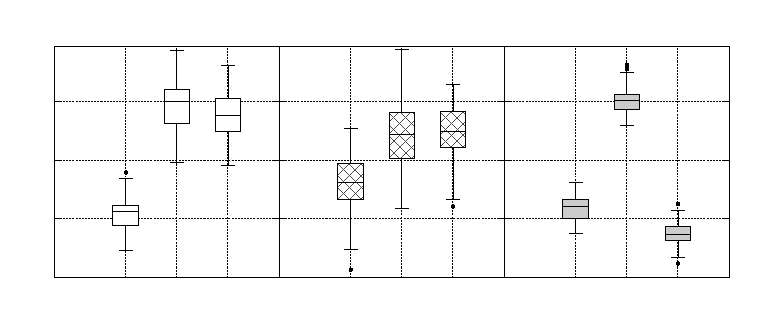
\includegraphics[width={360.00bp},height={144.00bp}]{Fat_path}}%
    \gplfronttext
  \end{picture}%
\endgroup
}}
    \caption{fat-tree}
    \label{fig:time:fat}
  \end{subfigure}
   \begin{subfigure}[b]{0.79\linewidth}
    \resizebox{\textwidth}{!}{\footnotesize{% GNUPLOT: LaTeX picture with Postscript
\begingroup
  \fontfamily{Times-Roman}%
  \selectfont
  \makeatletter
  \providecommand\color[2][]{%
    \GenericError{(gnuplot) \space\space\space\@spaces}{%
      Package color not loaded in conjunction with
      terminal option `colourtext'%
    }{See the gnuplot documentation for explanation.%
    }{Either use 'blacktext' in gnuplot or load the package
      color.sty in LaTeX.}%
    \renewcommand\color[2][]{}%
  }%
  \providecommand\includegraphics[2][]{%
    \GenericError{(gnuplot) \space\space\space\@spaces}{%
      Package graphicx or graphics not loaded%
    }{See the gnuplot documentation for explanation.%
    }{The gnuplot epslatex terminal needs graphicx.sty or graphics.sty.}%
    \renewcommand\includegraphics[2][]{}%
  }%
  \providecommand\rotatebox[2]{#2}%
  \@ifundefined{ifGPcolor}{%
    \newif\ifGPcolor
    \GPcolortrue
  }{}%
  \@ifundefined{ifGPblacktext}{%
    \newif\ifGPblacktext
    \GPblacktexttrue
  }{}%
  % define a \g@addto@macro without @ in the name:
  \let\gplgaddtomacro\g@addto@macro
  % define empty templates for all commands taking text:
  \gdef\gplbacktext{}%
  \gdef\gplfronttext{}%
  \makeatother
  \ifGPblacktext
    % no textcolor at all
    \def\colorrgb#1{}%
    \def\colorgray#1{}%
  \else
    % gray or color?
    \ifGPcolor
      \def\colorrgb#1{\color[rgb]{#1}}%
      \def\colorgray#1{\color[gray]{#1}}%
      \expandafter\def\csname LTw\endcsname{\color{white}}%
      \expandafter\def\csname LTb\endcsname{\color{black}}%
      \expandafter\def\csname LTa\endcsname{\color{black}}%
      \expandafter\def\csname LT0\endcsname{\color[rgb]{1,0,0}}%
      \expandafter\def\csname LT1\endcsname{\color[rgb]{0,1,0}}%
      \expandafter\def\csname LT2\endcsname{\color[rgb]{0,0,1}}%
      \expandafter\def\csname LT3\endcsname{\color[rgb]{1,0,1}}%
      \expandafter\def\csname LT4\endcsname{\color[rgb]{0,1,1}}%
      \expandafter\def\csname LT5\endcsname{\color[rgb]{1,1,0}}%
      \expandafter\def\csname LT6\endcsname{\color[rgb]{0,0,0}}%
      \expandafter\def\csname LT7\endcsname{\color[rgb]{1,0.3,0}}%
      \expandafter\def\csname LT8\endcsname{\color[rgb]{0.5,0.5,0.5}}%
    \else
      % gray
      \def\colorrgb#1{\color{black}}%
      \def\colorgray#1{\color[gray]{#1}}%
      \expandafter\def\csname LTw\endcsname{\color{white}}%
      \expandafter\def\csname LTb\endcsname{\color{black}}%
      \expandafter\def\csname LTa\endcsname{\color{black}}%
      \expandafter\def\csname LT0\endcsname{\color{black}}%
      \expandafter\def\csname LT1\endcsname{\color{black}}%
      \expandafter\def\csname LT2\endcsname{\color{black}}%
      \expandafter\def\csname LT3\endcsname{\color{black}}%
      \expandafter\def\csname LT4\endcsname{\color{black}}%
      \expandafter\def\csname LT5\endcsname{\color{black}}%
      \expandafter\def\csname LT6\endcsname{\color{black}}%
      \expandafter\def\csname LT7\endcsname{\color{black}}%
      \expandafter\def\csname LT8\endcsname{\color{black}}%
    \fi
  \fi
    \setlength{\unitlength}{0.0500bp}%
    \ifx\gptboxheight\undefined%
      \newlength{\gptboxheight}%
      \newlength{\gptboxwidth}%
      \newsavebox{\gptboxtext}%
    \fi%
    \setlength{\fboxrule}{0.5pt}%
    \setlength{\fboxsep}{1pt}%
\begin{picture}(7200.00,2880.00)%
    \gplgaddtomacro\gplbacktext{%
      \csname LTb\endcsname%%
      \put(782,528){\makebox(0,0)[r]{\strut{}$1900$}}%
      \csname LTb\endcsname%%
      \put(782,1089){\makebox(0,0)[r]{\strut{}$2100$}}%
      \csname LTb\endcsname%%
      \put(782,1651){\makebox(0,0)[r]{\strut{}$2300$}}%
      \csname LTb\endcsname%%
      \put(782,2212){\makebox(0,0)[r]{\strut{}$2500$}}%
      \csname LTb\endcsname%%
      \put(1126,242){\rotatebox{25}{\makebox(0,0)[r]{\strut{}SCC}}}%
      \csname LTb\endcsname%%
      \put(1617,242){\rotatebox{25}{\makebox(0,0)[r]{\strut{}CU}}}%
      \csname LTb\endcsname%%
      \put(2107,242){\rotatebox{25}{\makebox(0,0)[r]{\strut{}RWC}}}%
    }%
    \gplgaddtomacro\gplfronttext{%
      \csname LTb\endcsname%%
      \put(126,1482){\rotatebox{-270}{\makebox(0,0){\strut{}Time (ms)}}}%
      \put(1439,2701){\makebox(0,0){\strut{}Nimble}}%
    }%
    \gplgaddtomacro\gplbacktext{%
      \csname LTb\endcsname%%
      \put(2942,528){\makebox(0,0)[r]{\strut{}$2600$}}%
      \csname LTb\endcsname%%
      \put(2942,1089){\makebox(0,0)[r]{\strut{}$3000$}}%
      \csname LTb\endcsname%%
      \put(2942,1651){\makebox(0,0)[r]{\strut{}$3400$}}%
      \csname LTb\endcsname%%
      \put(2942,2212){\makebox(0,0)[r]{\strut{}$3800$}}%
      \csname LTb\endcsname%%
      \put(3286,242){\rotatebox{25}{\makebox(0,0)[r]{\strut{}SCC}}}%
      \csname LTb\endcsname%%
      \put(3777,242){\rotatebox{25}{\makebox(0,0)[r]{\strut{}CU}}}%
      \csname LTb\endcsname%%
      \put(4267,242){\rotatebox{25}{\makebox(0,0)[r]{\strut{}RWC}}}%
    }%
    \gplgaddtomacro\gplfronttext{%
      \csname LTb\endcsname%%
      \put(3599,2701){\makebox(0,0){\strut{}SwingState}}%
    }%
    \gplgaddtomacro\gplbacktext{%
      \csname LTb\endcsname%%
      \put(5102,528){\makebox(0,0)[r]{\strut{}$6600$}}%
      \csname LTb\endcsname%%
      \put(5102,1089){\makebox(0,0)[r]{\strut{}$7600$}}%
      \csname LTb\endcsname%%
      \put(5102,1651){\makebox(0,0)[r]{\strut{}$8600$}}%
      \csname LTb\endcsname%%
      \put(5102,2212){\makebox(0,0)[r]{\strut{}$9600$}}%
      \csname LTb\endcsname%%
      \put(5446,242){\rotatebox{25}{\makebox(0,0)[r]{\strut{}SCC}}}%
      \csname LTb\endcsname%%
      \put(5937,242){\rotatebox{25}{\makebox(0,0)[r]{\strut{}CU}}}%
      \csname LTb\endcsname%%
      \put(6427,242){\rotatebox{25}{\makebox(0,0)[r]{\strut{}RWC}}}%
    }%
    \gplgaddtomacro\gplfronttext{%
      \csname LTb\endcsname%%
      \put(5759,2701){\makebox(0,0){\strut{}OpenNF}}%
    }%
    \gplbacktext
    \put(0,0){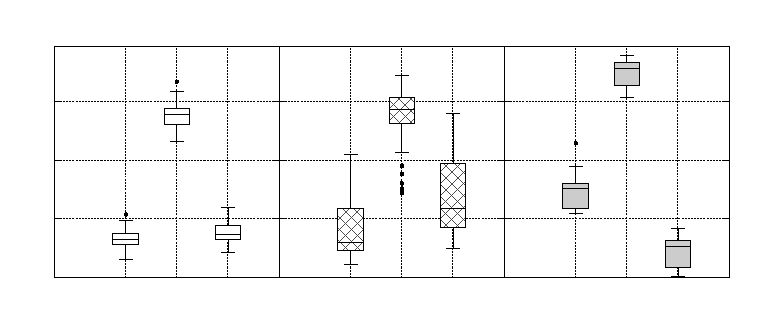
\includegraphics{Forthnet_path}}%
    \gplfronttext
  \end{picture}%
\endgroup
}}
    \caption{Forthnet}
    \label{fig:time:forthnet}
  \end{subfigure}
\caption{NF migration and path change times}
\label{fig:time}
\end{figure}



\iffalse
\begin{figure}[h!]
\centering
\begin{minipage}{0.49\linewidth}
   \begin{subfigure}[b]{0.99\linewidth}
    \resizebox{\textwidth}{!}{\footnotesize{% GNUPLOT: LaTeX picture with Postscript
\begingroup
  \fontfamily{Times-Roman}%
  \selectfont
  \makeatletter
  \providecommand\color[2][]{%
    \GenericError{(gnuplot) \space\space\space\@spaces}{%
      Package color not loaded in conjunction with
      terminal option `colourtext'%
    }{See the gnuplot documentation for explanation.%
    }{Either use 'blacktext' in gnuplot or load the package
      color.sty in LaTeX.}%
    \renewcommand\color[2][]{}%
  }%
  \providecommand\includegraphics[2][]{%
    \GenericError{(gnuplot) \space\space\space\@spaces}{%
      Package graphicx or graphics not loaded%
    }{See the gnuplot documentation for explanation.%
    }{The gnuplot epslatex terminal needs graphicx.sty or graphics.sty.}%
    \renewcommand\includegraphics[2][]{}%
  }%
  \providecommand\rotatebox[2]{#2}%
  \@ifundefined{ifGPcolor}{%
    \newif\ifGPcolor
    \GPcolortrue
  }{}%
  \@ifundefined{ifGPblacktext}{%
    \newif\ifGPblacktext
    \GPblacktexttrue
  }{}%
  % define a \g@addto@macro without @ in the name:
  \let\gplgaddtomacro\g@addto@macro
  % define empty templates for all commands taking text:
  \gdef\gplbacktext{}%
  \gdef\gplfronttext{}%
  \makeatother
  \ifGPblacktext
    % no textcolor at all
    \def\colorrgb#1{}%
    \def\colorgray#1{}%
  \else
    % gray or color?
    \ifGPcolor
      \def\colorrgb#1{\color[rgb]{#1}}%
      \def\colorgray#1{\color[gray]{#1}}%
      \expandafter\def\csname LTw\endcsname{\color{white}}%
      \expandafter\def\csname LTb\endcsname{\color{black}}%
      \expandafter\def\csname LTa\endcsname{\color{black}}%
      \expandafter\def\csname LT0\endcsname{\color[rgb]{1,0,0}}%
      \expandafter\def\csname LT1\endcsname{\color[rgb]{0,1,0}}%
      \expandafter\def\csname LT2\endcsname{\color[rgb]{0,0,1}}%
      \expandafter\def\csname LT3\endcsname{\color[rgb]{1,0,1}}%
      \expandafter\def\csname LT4\endcsname{\color[rgb]{0,1,1}}%
      \expandafter\def\csname LT5\endcsname{\color[rgb]{1,1,0}}%
      \expandafter\def\csname LT6\endcsname{\color[rgb]{0,0,0}}%
      \expandafter\def\csname LT7\endcsname{\color[rgb]{1,0.3,0}}%
      \expandafter\def\csname LT8\endcsname{\color[rgb]{0.5,0.5,0.5}}%
    \else
      % gray
      \def\colorrgb#1{\color{black}}%
      \def\colorgray#1{\color[gray]{#1}}%
      \expandafter\def\csname LTw\endcsname{\color{white}}%
      \expandafter\def\csname LTb\endcsname{\color{black}}%
      \expandafter\def\csname LTa\endcsname{\color{black}}%
      \expandafter\def\csname LT0\endcsname{\color{black}}%
      \expandafter\def\csname LT1\endcsname{\color{black}}%
      \expandafter\def\csname LT2\endcsname{\color{black}}%
      \expandafter\def\csname LT3\endcsname{\color{black}}%
      \expandafter\def\csname LT4\endcsname{\color{black}}%
      \expandafter\def\csname LT5\endcsname{\color{black}}%
      \expandafter\def\csname LT6\endcsname{\color{black}}%
      \expandafter\def\csname LT7\endcsname{\color{black}}%
      \expandafter\def\csname LT8\endcsname{\color{black}}%
    \fi
  \fi
    \setlength{\unitlength}{0.0500bp}%
    \ifx\gptboxheight\undefined%
      \newlength{\gptboxheight}%
      \newlength{\gptboxwidth}%
      \newsavebox{\gptboxtext}%
    \fi%
    \setlength{\fboxrule}{0.5pt}%
    \setlength{\fboxsep}{1pt}%
\begin{picture}(5760.00,2880.00)%
    \gplgaddtomacro\gplbacktext{%
      \csname LTb\endcsname%%
      \put(686,554){\makebox(0,0)[r]{\strut{}$12250$}}%
      \put(686,1043){\makebox(0,0)[r]{\strut{}$12500$}}%
      \put(686,1532){\makebox(0,0)[r]{\strut{}$12750$}}%
      \put(686,2021){\makebox(0,0)[r]{\strut{}$13000$}}%
      \put(686,2510){\makebox(0,0)[r]{\strut{}$13250$}}%
      \put(770,252){\makebox(0,0){\strut{}$0$}}%
      \put(1260,252){\makebox(0,0){\strut{}$500$}}%
      \put(1750,252){\makebox(0,0){\strut{}$1000$}}%
      \put(2240,252){\makebox(0,0){\strut{}$1500$}}%
      \put(2730,252){\makebox(0,0){\strut{}$2000$}}%
      \put(3220,252){\makebox(0,0){\strut{}$2500$}}%
      \put(3710,252){\makebox(0,0){\strut{}$3000$}}%
      \put(4200,252){\makebox(0,0){\strut{}$3500$}}%
      \put(4690,252){\makebox(0,0){\strut{}$4000$}}%
      \put(5180,252){\makebox(0,0){\strut{}$4500$}}%
    }%
    \gplgaddtomacro\gplfronttext{%
      \csname LTb\endcsname%%
      \put(168,1474){\rotatebox{-270}{\makebox(0,0){\strut{}Total number of rules}}}%
      \put(3138,98){\makebox(0,0){\strut{}Time (ms)}}%
      \csname LTb\endcsname%%
      \put(1133,2733){\makebox(0,0)[l]{\strut{}SCC+Nimble}}%
      \csname LTb\endcsname%%
      \put(2792,2733){\makebox(0,0)[l]{\strut{}SCC+OpenNF}}%
      \csname LTb\endcsname%%
      \put(4451,2733){\makebox(0,0)[l]{\strut{}SCC+SwingState}}%
    }%
    \gplbacktext
    \put(0,0){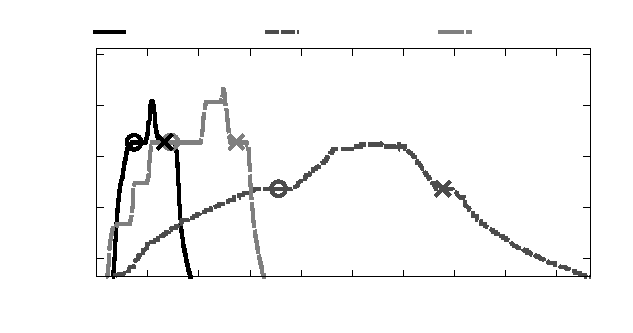
\includegraphics{SCCRuleFat}}%
    \gplfronttext
  \end{picture}%
\endgroup
}}
    \caption{SCC}
    \label{fig:rule_number:fat:scc}
  \end{subfigure}
  \par\bigskip
  \begin{subfigure}[b]{0.99\linewidth}
    \resizebox{\textwidth}{!}{\footnotesize{% GNUPLOT: LaTeX picture with Postscript
\begingroup
  \fontfamily{Times-Roman}%
  \selectfont
  \makeatletter
  \providecommand\color[2][]{%
    \GenericError{(gnuplot) \space\space\space\@spaces}{%
      Package color not loaded in conjunction with
      terminal option `colourtext'%
    }{See the gnuplot documentation for explanation.%
    }{Either use 'blacktext' in gnuplot or load the package
      color.sty in LaTeX.}%
    \renewcommand\color[2][]{}%
  }%
  \providecommand\includegraphics[2][]{%
    \GenericError{(gnuplot) \space\space\space\@spaces}{%
      Package graphicx or graphics not loaded%
    }{See the gnuplot documentation for explanation.%
    }{The gnuplot epslatex terminal needs graphicx.sty or graphics.sty.}%
    \renewcommand\includegraphics[2][]{}%
  }%
  \providecommand\rotatebox[2]{#2}%
  \@ifundefined{ifGPcolor}{%
    \newif\ifGPcolor
    \GPcolortrue
  }{}%
  \@ifundefined{ifGPblacktext}{%
    \newif\ifGPblacktext
    \GPblacktexttrue
  }{}%
  % define a \g@addto@macro without @ in the name:
  \let\gplgaddtomacro\g@addto@macro
  % define empty templates for all commands taking text:
  \gdef\gplbacktext{}%
  \gdef\gplfronttext{}%
  \makeatother
  \ifGPblacktext
    % no textcolor at all
    \def\colorrgb#1{}%
    \def\colorgray#1{}%
  \else
    % gray or color?
    \ifGPcolor
      \def\colorrgb#1{\color[rgb]{#1}}%
      \def\colorgray#1{\color[gray]{#1}}%
      \expandafter\def\csname LTw\endcsname{\color{white}}%
      \expandafter\def\csname LTb\endcsname{\color{black}}%
      \expandafter\def\csname LTa\endcsname{\color{black}}%
      \expandafter\def\csname LT0\endcsname{\color[rgb]{1,0,0}}%
      \expandafter\def\csname LT1\endcsname{\color[rgb]{0,1,0}}%
      \expandafter\def\csname LT2\endcsname{\color[rgb]{0,0,1}}%
      \expandafter\def\csname LT3\endcsname{\color[rgb]{1,0,1}}%
      \expandafter\def\csname LT4\endcsname{\color[rgb]{0,1,1}}%
      \expandafter\def\csname LT5\endcsname{\color[rgb]{1,1,0}}%
      \expandafter\def\csname LT6\endcsname{\color[rgb]{0,0,0}}%
      \expandafter\def\csname LT7\endcsname{\color[rgb]{1,0.3,0}}%
      \expandafter\def\csname LT8\endcsname{\color[rgb]{0.5,0.5,0.5}}%
    \else
      % gray
      \def\colorrgb#1{\color{black}}%
      \def\colorgray#1{\color[gray]{#1}}%
      \expandafter\def\csname LTw\endcsname{\color{white}}%
      \expandafter\def\csname LTb\endcsname{\color{black}}%
      \expandafter\def\csname LTa\endcsname{\color{black}}%
      \expandafter\def\csname LT0\endcsname{\color{black}}%
      \expandafter\def\csname LT1\endcsname{\color{black}}%
      \expandafter\def\csname LT2\endcsname{\color{black}}%
      \expandafter\def\csname LT3\endcsname{\color{black}}%
      \expandafter\def\csname LT4\endcsname{\color{black}}%
      \expandafter\def\csname LT5\endcsname{\color{black}}%
      \expandafter\def\csname LT6\endcsname{\color{black}}%
      \expandafter\def\csname LT7\endcsname{\color{black}}%
      \expandafter\def\csname LT8\endcsname{\color{black}}%
    \fi
  \fi
    \setlength{\unitlength}{0.0500bp}%
    \ifx\gptboxheight\undefined%
      \newlength{\gptboxheight}%
      \newlength{\gptboxwidth}%
      \newsavebox{\gptboxtext}%
    \fi%
    \setlength{\fboxrule}{0.5pt}%
    \setlength{\fboxsep}{1pt}%
\begin{picture}(5760.00,2880.00)%
    \gplgaddtomacro\gplbacktext{%
      \csname LTb\endcsname%%
      \put(686,588){\makebox(0,0)[r]{\strut{}$12300$}}%
      \put(686,1039){\makebox(0,0)[r]{\strut{}$12600$}}%
      \put(686,1490){\makebox(0,0)[r]{\strut{}$12900$}}%
      \put(686,1940){\makebox(0,0)[r]{\strut{}$13200$}}%
      \put(686,2391){\makebox(0,0)[r]{\strut{}$13500$}}%
      \put(770,252){\makebox(0,0){\strut{}$0$}}%
      \put(1557,252){\makebox(0,0){\strut{}$1000$}}%
      \put(2344,252){\makebox(0,0){\strut{}$2000$}}%
      \put(3130,252){\makebox(0,0){\strut{}$3000$}}%
      \put(3917,252){\makebox(0,0){\strut{}$4000$}}%
      \put(4704,252){\makebox(0,0){\strut{}$5000$}}%
      \put(5491,252){\makebox(0,0){\strut{}$6000$}}%
    }%
    \gplgaddtomacro\gplfronttext{%
      \csname LTb\endcsname%%
      \put(168,1474){\rotatebox{-270}{\makebox(0,0){\strut{}Total number of rules}}}%
      \put(3138,98){\makebox(0,0){\strut{}Time (ms)}}%
      \csname LTb\endcsname%%
      \put(1259,2733){\makebox(0,0)[l]{\strut{}CU+Nimble}}%
      \csname LTb\endcsname%%
      \put(2834,2733){\makebox(0,0)[l]{\strut{}CU+OpenNF}}%
      \csname LTb\endcsname%%
      \put(4409,2733){\makebox(0,0)[l]{\strut{}CU+SwingState}}%
    }%
    \gplbacktext
    \put(0,0){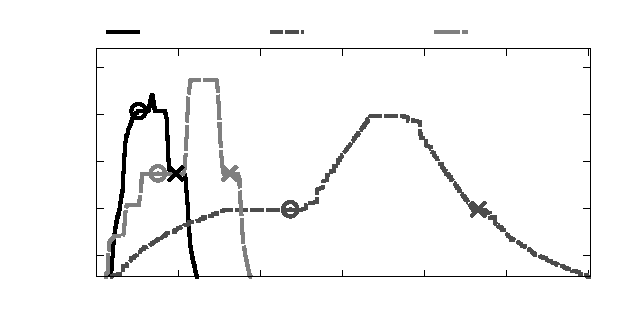
\includegraphics{CURuleFat}}%
    \gplfronttext
  \end{picture}%
\endgroup
}}
    \caption{CU}
    \label{fig:rule_number:fat:scc}
  \end{subfigure}
  \par\bigskip
  \begin{subfigure}[b]{0.99\linewidth}
    \resizebox{\textwidth}{!}{\footnotesize{% GNUPLOT: LaTeX picture with Postscript
\begingroup
  \fontfamily{Times-Roman}%
  \selectfont
  \makeatletter
  \providecommand\color[2][]{%
    \GenericError{(gnuplot) \space\space\space\@spaces}{%
      Package color not loaded in conjunction with
      terminal option `colourtext'%
    }{See the gnuplot documentation for explanation.%
    }{Either use 'blacktext' in gnuplot or load the package
      color.sty in LaTeX.}%
    \renewcommand\color[2][]{}%
  }%
  \providecommand\includegraphics[2][]{%
    \GenericError{(gnuplot) \space\space\space\@spaces}{%
      Package graphicx or graphics not loaded%
    }{See the gnuplot documentation for explanation.%
    }{The gnuplot epslatex terminal needs graphicx.sty or graphics.sty.}%
    \renewcommand\includegraphics[2][]{}%
  }%
  \providecommand\rotatebox[2]{#2}%
  \@ifundefined{ifGPcolor}{%
    \newif\ifGPcolor
    \GPcolortrue
  }{}%
  \@ifundefined{ifGPblacktext}{%
    \newif\ifGPblacktext
    \GPblacktexttrue
  }{}%
  % define a \g@addto@macro without @ in the name:
  \let\gplgaddtomacro\g@addto@macro
  % define empty templates for all commands taking text:
  \gdef\gplbacktext{}%
  \gdef\gplfronttext{}%
  \makeatother
  \ifGPblacktext
    % no textcolor at all
    \def\colorrgb#1{}%
    \def\colorgray#1{}%
  \else
    % gray or color?
    \ifGPcolor
      \def\colorrgb#1{\color[rgb]{#1}}%
      \def\colorgray#1{\color[gray]{#1}}%
      \expandafter\def\csname LTw\endcsname{\color{white}}%
      \expandafter\def\csname LTb\endcsname{\color{black}}%
      \expandafter\def\csname LTa\endcsname{\color{black}}%
      \expandafter\def\csname LT0\endcsname{\color[rgb]{1,0,0}}%
      \expandafter\def\csname LT1\endcsname{\color[rgb]{0,1,0}}%
      \expandafter\def\csname LT2\endcsname{\color[rgb]{0,0,1}}%
      \expandafter\def\csname LT3\endcsname{\color[rgb]{1,0,1}}%
      \expandafter\def\csname LT4\endcsname{\color[rgb]{0,1,1}}%
      \expandafter\def\csname LT5\endcsname{\color[rgb]{1,1,0}}%
      \expandafter\def\csname LT6\endcsname{\color[rgb]{0,0,0}}%
      \expandafter\def\csname LT7\endcsname{\color[rgb]{1,0.3,0}}%
      \expandafter\def\csname LT8\endcsname{\color[rgb]{0.5,0.5,0.5}}%
    \else
      % gray
      \def\colorrgb#1{\color{black}}%
      \def\colorgray#1{\color[gray]{#1}}%
      \expandafter\def\csname LTw\endcsname{\color{white}}%
      \expandafter\def\csname LTb\endcsname{\color{black}}%
      \expandafter\def\csname LTa\endcsname{\color{black}}%
      \expandafter\def\csname LT0\endcsname{\color{black}}%
      \expandafter\def\csname LT1\endcsname{\color{black}}%
      \expandafter\def\csname LT2\endcsname{\color{black}}%
      \expandafter\def\csname LT3\endcsname{\color{black}}%
      \expandafter\def\csname LT4\endcsname{\color{black}}%
      \expandafter\def\csname LT5\endcsname{\color{black}}%
      \expandafter\def\csname LT6\endcsname{\color{black}}%
      \expandafter\def\csname LT7\endcsname{\color{black}}%
      \expandafter\def\csname LT8\endcsname{\color{black}}%
    \fi
  \fi
    \setlength{\unitlength}{0.0500bp}%
    \ifx\gptboxheight\undefined%
      \newlength{\gptboxheight}%
      \newlength{\gptboxwidth}%
      \newsavebox{\gptboxtext}%
    \fi%
    \setlength{\fboxrule}{0.5pt}%
    \setlength{\fboxsep}{1pt}%
\begin{picture}(5760.00,2880.00)%
    \gplgaddtomacro\gplbacktext{%
      \csname LTb\endcsname%%
      \put(686,547){\makebox(0,0)[r]{\strut{}$12250$}}%
      \put(686,1015){\makebox(0,0)[r]{\strut{}$12500$}}%
      \put(686,1484){\makebox(0,0)[r]{\strut{}$12750$}}%
      \put(686,1952){\makebox(0,0)[r]{\strut{}$13000$}}%
      \put(686,2421){\makebox(0,0)[r]{\strut{}$13250$}}%
      \put(770,252){\makebox(0,0){\strut{}$0$}}%
      \put(1272,252){\makebox(0,0){\strut{}$500$}}%
      \put(1775,252){\makebox(0,0){\strut{}$1000$}}%
      \put(2277,252){\makebox(0,0){\strut{}$1500$}}%
      \put(2780,252){\makebox(0,0){\strut{}$2000$}}%
      \put(3282,252){\makebox(0,0){\strut{}$2500$}}%
      \put(3785,252){\makebox(0,0){\strut{}$3000$}}%
      \put(4287,252){\makebox(0,0){\strut{}$3500$}}%
      \put(4790,252){\makebox(0,0){\strut{}$4000$}}%
      \put(5292,252){\makebox(0,0){\strut{}$4500$}}%
    }%
    \gplgaddtomacro\gplfronttext{%
      \csname LTb\endcsname%%
      \put(168,1474){\rotatebox{-270}{\makebox(0,0){\strut{}Total number of rules}}}%
      \put(3138,98){\makebox(0,0){\strut{}Time (ms)}}%
      \csname LTb\endcsname%%
      \put(1133,2733){\makebox(0,0)[l]{\strut{}RWC+Nimble}}%
      \csname LTb\endcsname%%
      \put(2792,2733){\makebox(0,0)[l]{\strut{}RWC+OpenNF}}%
      \csname LTb\endcsname%%
      \put(4451,2733){\makebox(0,0)[l]{\strut{}RWC+SwingState}}%
    }%
    \gplbacktext
    \put(0,0){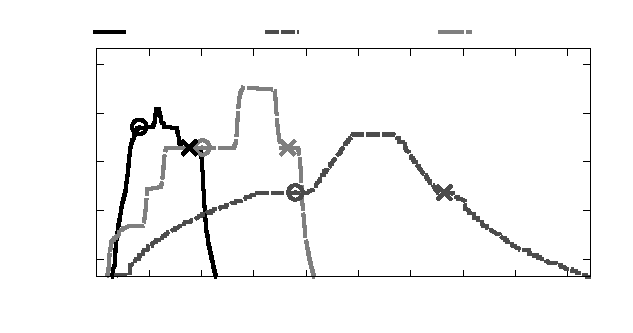
\includegraphics{RWCRuleFat}}%
    \gplfronttext
  \end{picture}%
\endgroup
}}
    \caption{\ourRouteUpdateName}
    \label{fig:rule_number:fat:cu}
  \end{subfigure}
  \caption{Rules in the network during 100 path changes and
    accompanying NF migrations for fat-tree topology; markers show
    completion of path changes ($\times$) and NF migrations
    ({\LARGE $\circ$})}
\label{fig:rule_number:fat}
\end{minipage}
\centering
\begin{minipage}{0.49\linewidth}
   \begin{subfigure}[b]{0.99\linewidth}
    \resizebox{\textwidth}{!}{\footnotesize{% GNUPLOT: LaTeX picture with Postscript
\begingroup
  \fontfamily{Times-Roman}%
  \selectfont
  \makeatletter
  \providecommand\color[2][]{%
    \GenericError{(gnuplot) \space\space\space\@spaces}{%
      Package color not loaded in conjunction with
      terminal option `colourtext'%
    }{See the gnuplot documentation for explanation.%
    }{Either use 'blacktext' in gnuplot or load the package
      color.sty in LaTeX.}%
    \renewcommand\color[2][]{}%
  }%
  \providecommand\includegraphics[2][]{%
    \GenericError{(gnuplot) \space\space\space\@spaces}{%
      Package graphicx or graphics not loaded%
    }{See the gnuplot documentation for explanation.%
    }{The gnuplot epslatex terminal needs graphicx.sty or graphics.sty.}%
    \renewcommand\includegraphics[2][]{}%
  }%
  \providecommand\rotatebox[2]{#2}%
  \@ifundefined{ifGPcolor}{%
    \newif\ifGPcolor
    \GPcolortrue
  }{}%
  \@ifundefined{ifGPblacktext}{%
    \newif\ifGPblacktext
    \GPblacktexttrue
  }{}%
  % define a \g@addto@macro without @ in the name:
  \let\gplgaddtomacro\g@addto@macro
  % define empty templates for all commands taking text:
  \gdef\gplbacktext{}%
  \gdef\gplfronttext{}%
  \makeatother
  \ifGPblacktext
    % no textcolor at all
    \def\colorrgb#1{}%
    \def\colorgray#1{}%
  \else
    % gray or color?
    \ifGPcolor
      \def\colorrgb#1{\color[rgb]{#1}}%
      \def\colorgray#1{\color[gray]{#1}}%
      \expandafter\def\csname LTw\endcsname{\color{white}}%
      \expandafter\def\csname LTb\endcsname{\color{black}}%
      \expandafter\def\csname LTa\endcsname{\color{black}}%
      \expandafter\def\csname LT0\endcsname{\color[rgb]{1,0,0}}%
      \expandafter\def\csname LT1\endcsname{\color[rgb]{0,1,0}}%
      \expandafter\def\csname LT2\endcsname{\color[rgb]{0,0,1}}%
      \expandafter\def\csname LT3\endcsname{\color[rgb]{1,0,1}}%
      \expandafter\def\csname LT4\endcsname{\color[rgb]{0,1,1}}%
      \expandafter\def\csname LT5\endcsname{\color[rgb]{1,1,0}}%
      \expandafter\def\csname LT6\endcsname{\color[rgb]{0,0,0}}%
      \expandafter\def\csname LT7\endcsname{\color[rgb]{1,0.3,0}}%
      \expandafter\def\csname LT8\endcsname{\color[rgb]{0.5,0.5,0.5}}%
    \else
      % gray
      \def\colorrgb#1{\color{black}}%
      \def\colorgray#1{\color[gray]{#1}}%
      \expandafter\def\csname LTw\endcsname{\color{white}}%
      \expandafter\def\csname LTb\endcsname{\color{black}}%
      \expandafter\def\csname LTa\endcsname{\color{black}}%
      \expandafter\def\csname LT0\endcsname{\color{black}}%
      \expandafter\def\csname LT1\endcsname{\color{black}}%
      \expandafter\def\csname LT2\endcsname{\color{black}}%
      \expandafter\def\csname LT3\endcsname{\color{black}}%
      \expandafter\def\csname LT4\endcsname{\color{black}}%
      \expandafter\def\csname LT5\endcsname{\color{black}}%
      \expandafter\def\csname LT6\endcsname{\color{black}}%
      \expandafter\def\csname LT7\endcsname{\color{black}}%
      \expandafter\def\csname LT8\endcsname{\color{black}}%
    \fi
  \fi
    \setlength{\unitlength}{0.0500bp}%
    \ifx\gptboxheight\undefined%
      \newlength{\gptboxheight}%
      \newlength{\gptboxwidth}%
      \newsavebox{\gptboxtext}%
    \fi%
    \setlength{\fboxrule}{0.5pt}%
    \setlength{\fboxsep}{1pt}%
\begin{picture}(5760.00,2880.00)%
    \gplgaddtomacro\gplbacktext{%
      \csname LTb\endcsname%%
      \put(686,553){\makebox(0,0)[r]{\strut{}$12000$}}%
      \put(686,1005){\makebox(0,0)[r]{\strut{}$12400$}}%
      \put(686,1456){\makebox(0,0)[r]{\strut{}$12800$}}%
      \put(686,1908){\makebox(0,0)[r]{\strut{}$13200$}}%
      \put(686,2360){\makebox(0,0)[r]{\strut{}$13600$}}%
      \put(770,252){\makebox(0,0){\strut{}$0$}}%
      \put(1627,252){\makebox(0,0){\strut{}$2000$}}%
      \put(2483,252){\makebox(0,0){\strut{}$4000$}}%
      \put(3340,252){\makebox(0,0){\strut{}$6000$}}%
      \put(4197,252){\makebox(0,0){\strut{}$8000$}}%
      \put(5053,252){\makebox(0,0){\strut{}$10000$}}%
    }%
    \gplgaddtomacro\gplfronttext{%
      \csname LTb\endcsname%%
      \put(168,1474){\rotatebox{-270}{\makebox(0,0){\strut{}Total number of rules}}}%
      \put(3138,98){\makebox(0,0){\strut{}Time (ms)}}%
      \csname LTb\endcsname%%
      \put(1133,2733){\makebox(0,0)[l]{\strut{}SCC+Nimble}}%
      \csname LTb\endcsname%%
      \put(2792,2733){\makebox(0,0)[l]{\strut{}SCC+OpenNF}}%
      \csname LTb\endcsname%%
      \put(4451,2733){\makebox(0,0)[l]{\strut{}SCC+SwingState}}%
    }%
    \gplbacktext
    \put(0,0){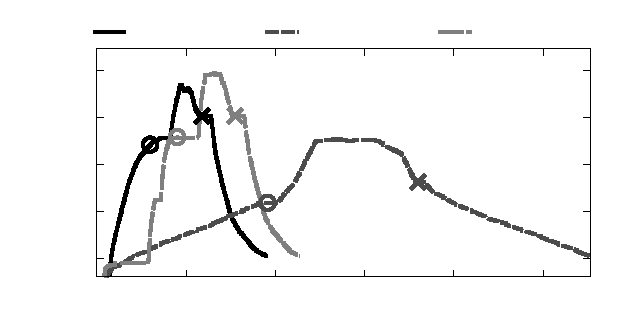
\includegraphics{SCCRuleForthnet}}%
    \gplfronttext
  \end{picture}%
\endgroup
}}
    \caption{SCC}
    \label{fig:rule_number:Forthnet:scc}
  \end{subfigure}
  \par\bigskip
  \begin{subfigure}[b]{0.99\linewidth}
    \resizebox{\textwidth}{!}{\footnotesize{% GNUPLOT: LaTeX picture with Postscript
\begingroup
  \fontfamily{Times-Roman}%
  \selectfont
  \makeatletter
  \providecommand\color[2][]{%
    \GenericError{(gnuplot) \space\space\space\@spaces}{%
      Package color not loaded in conjunction with
      terminal option `colourtext'%
    }{See the gnuplot documentation for explanation.%
    }{Either use 'blacktext' in gnuplot or load the package
      color.sty in LaTeX.}%
    \renewcommand\color[2][]{}%
  }%
  \providecommand\includegraphics[2][]{%
    \GenericError{(gnuplot) \space\space\space\@spaces}{%
      Package graphicx or graphics not loaded%
    }{See the gnuplot documentation for explanation.%
    }{The gnuplot epslatex terminal needs graphicx.sty or graphics.sty.}%
    \renewcommand\includegraphics[2][]{}%
  }%
  \providecommand\rotatebox[2]{#2}%
  \@ifundefined{ifGPcolor}{%
    \newif\ifGPcolor
    \GPcolortrue
  }{}%
  \@ifundefined{ifGPblacktext}{%
    \newif\ifGPblacktext
    \GPblacktexttrue
  }{}%
  % define a \g@addto@macro without @ in the name:
  \let\gplgaddtomacro\g@addto@macro
  % define empty templates for all commands taking text:
  \gdef\gplbacktext{}%
  \gdef\gplfronttext{}%
  \makeatother
  \ifGPblacktext
    % no textcolor at all
    \def\colorrgb#1{}%
    \def\colorgray#1{}%
  \else
    % gray or color?
    \ifGPcolor
      \def\colorrgb#1{\color[rgb]{#1}}%
      \def\colorgray#1{\color[gray]{#1}}%
      \expandafter\def\csname LTw\endcsname{\color{white}}%
      \expandafter\def\csname LTb\endcsname{\color{black}}%
      \expandafter\def\csname LTa\endcsname{\color{black}}%
      \expandafter\def\csname LT0\endcsname{\color[rgb]{1,0,0}}%
      \expandafter\def\csname LT1\endcsname{\color[rgb]{0,1,0}}%
      \expandafter\def\csname LT2\endcsname{\color[rgb]{0,0,1}}%
      \expandafter\def\csname LT3\endcsname{\color[rgb]{1,0,1}}%
      \expandafter\def\csname LT4\endcsname{\color[rgb]{0,1,1}}%
      \expandafter\def\csname LT5\endcsname{\color[rgb]{1,1,0}}%
      \expandafter\def\csname LT6\endcsname{\color[rgb]{0,0,0}}%
      \expandafter\def\csname LT7\endcsname{\color[rgb]{1,0.3,0}}%
      \expandafter\def\csname LT8\endcsname{\color[rgb]{0.5,0.5,0.5}}%
    \else
      % gray
      \def\colorrgb#1{\color{black}}%
      \def\colorgray#1{\color[gray]{#1}}%
      \expandafter\def\csname LTw\endcsname{\color{white}}%
      \expandafter\def\csname LTb\endcsname{\color{black}}%
      \expandafter\def\csname LTa\endcsname{\color{black}}%
      \expandafter\def\csname LT0\endcsname{\color{black}}%
      \expandafter\def\csname LT1\endcsname{\color{black}}%
      \expandafter\def\csname LT2\endcsname{\color{black}}%
      \expandafter\def\csname LT3\endcsname{\color{black}}%
      \expandafter\def\csname LT4\endcsname{\color{black}}%
      \expandafter\def\csname LT5\endcsname{\color{black}}%
      \expandafter\def\csname LT6\endcsname{\color{black}}%
      \expandafter\def\csname LT7\endcsname{\color{black}}%
      \expandafter\def\csname LT8\endcsname{\color{black}}%
    \fi
  \fi
    \setlength{\unitlength}{0.0500bp}%
    \ifx\gptboxheight\undefined%
      \newlength{\gptboxheight}%
      \newlength{\gptboxwidth}%
      \newsavebox{\gptboxtext}%
    \fi%
    \setlength{\fboxrule}{0.5pt}%
    \setlength{\fboxsep}{1pt}%
\begin{picture}(5760.00,2880.00)%
    \gplgaddtomacro\gplbacktext{%
      \csname LTb\endcsname%%
      \put(686,417){\makebox(0,0)[r]{\strut{}$11900$}}%
      \put(686,920){\makebox(0,0)[r]{\strut{}$12600$}}%
      \put(686,1422){\makebox(0,0)[r]{\strut{}$13300$}}%
      \put(686,1924){\makebox(0,0)[r]{\strut{}$14000$}}%
      \put(686,2427){\makebox(0,0)[r]{\strut{}$14700$}}%
      \put(770,252){\makebox(0,0){\strut{}$0$}}%
      \put(1509,252){\makebox(0,0){\strut{}$2000$}}%
      \put(2248,252){\makebox(0,0){\strut{}$4000$}}%
      \put(2986,252){\makebox(0,0){\strut{}$6000$}}%
      \put(3725,252){\makebox(0,0){\strut{}$8000$}}%
      \put(4464,252){\makebox(0,0){\strut{}$10000$}}%
      \put(5203,252){\makebox(0,0){\strut{}$12000$}}%
    }%
    \gplgaddtomacro\gplfronttext{%
      \csname LTb\endcsname%%
      \put(168,1474){\rotatebox{-270}{\makebox(0,0){\strut{}Total number of rules}}}%
      \put(3138,98){\makebox(0,0){\strut{}Time (ms)}}%
      \csname LTb\endcsname%%
      \put(1259,2733){\makebox(0,0)[l]{\strut{}CU+Nimble}}%
      \csname LTb\endcsname%%
      \put(2834,2733){\makebox(0,0)[l]{\strut{}CU+OpenNF}}%
      \csname LTb\endcsname%%
      \put(4409,2733){\makebox(0,0)[l]{\strut{}CU+SwingState}}%
    }%
    \gplbacktext
    \put(0,0){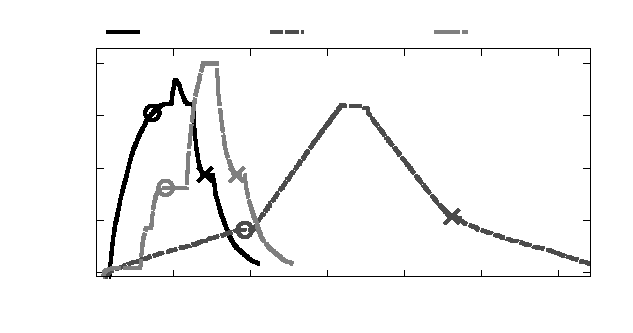
\includegraphics{CURuleForthnet}}%
    \gplfronttext
  \end{picture}%
\endgroup
}}
    \caption{CU}
    \label{fig:rule_number:Forthnet:scc}
  \end{subfigure}
  \par\bigskip
  \begin{subfigure}[b]{0.99\linewidth}
    \resizebox{\textwidth}{!}{\small{% GNUPLOT: LaTeX picture with Postscript
\begingroup
  \fontfamily{Times-Roman}%
  \selectfont
  \makeatletter
  \providecommand\color[2][]{%
    \GenericError{(gnuplot) \space\space\space\@spaces}{%
      Package color not loaded in conjunction with
      terminal option `colourtext'%
    }{See the gnuplot documentation for explanation.%
    }{Either use 'blacktext' in gnuplot or load the package
      color.sty in LaTeX.}%
    \renewcommand\color[2][]{}%
  }%
  \providecommand\includegraphics[2][]{%
    \GenericError{(gnuplot) \space\space\space\@spaces}{%
      Package graphicx or graphics not loaded%
    }{See the gnuplot documentation for explanation.%
    }{The gnuplot epslatex terminal needs graphicx.sty or graphics.sty.}%
    \renewcommand\includegraphics[2][]{}%
  }%
  \providecommand\rotatebox[2]{#2}%
  \@ifundefined{ifGPcolor}{%
    \newif\ifGPcolor
    \GPcolortrue
  }{}%
  \@ifundefined{ifGPblacktext}{%
    \newif\ifGPblacktext
    \GPblacktexttrue
  }{}%
  % define a \g@addto@macro without @ in the name:
  \let\gplgaddtomacro\g@addto@macro
  % define empty templates for all commands taking text:
  \gdef\gplbacktext{}%
  \gdef\gplfronttext{}%
  \makeatother
  \ifGPblacktext
    % no textcolor at all
    \def\colorrgb#1{}%
    \def\colorgray#1{}%
  \else
    % gray or color?
    \ifGPcolor
      \def\colorrgb#1{\color[rgb]{#1}}%
      \def\colorgray#1{\color[gray]{#1}}%
      \expandafter\def\csname LTw\endcsname{\color{white}}%
      \expandafter\def\csname LTb\endcsname{\color{black}}%
      \expandafter\def\csname LTa\endcsname{\color{black}}%
      \expandafter\def\csname LT0\endcsname{\color[rgb]{1,0,0}}%
      \expandafter\def\csname LT1\endcsname{\color[rgb]{0,1,0}}%
      \expandafter\def\csname LT2\endcsname{\color[rgb]{0,0,1}}%
      \expandafter\def\csname LT3\endcsname{\color[rgb]{1,0,1}}%
      \expandafter\def\csname LT4\endcsname{\color[rgb]{0,1,1}}%
      \expandafter\def\csname LT5\endcsname{\color[rgb]{1,1,0}}%
      \expandafter\def\csname LT6\endcsname{\color[rgb]{0,0,0}}%
      \expandafter\def\csname LT7\endcsname{\color[rgb]{1,0.3,0}}%
      \expandafter\def\csname LT8\endcsname{\color[rgb]{0.5,0.5,0.5}}%
    \else
      % gray
      \def\colorrgb#1{\color{black}}%
      \def\colorgray#1{\color[gray]{#1}}%
      \expandafter\def\csname LTw\endcsname{\color{white}}%
      \expandafter\def\csname LTb\endcsname{\color{black}}%
      \expandafter\def\csname LTa\endcsname{\color{black}}%
      \expandafter\def\csname LT0\endcsname{\color{black}}%
      \expandafter\def\csname LT1\endcsname{\color{black}}%
      \expandafter\def\csname LT2\endcsname{\color{black}}%
      \expandafter\def\csname LT3\endcsname{\color{black}}%
      \expandafter\def\csname LT4\endcsname{\color{black}}%
      \expandafter\def\csname LT5\endcsname{\color{black}}%
      \expandafter\def\csname LT6\endcsname{\color{black}}%
      \expandafter\def\csname LT7\endcsname{\color{black}}%
      \expandafter\def\csname LT8\endcsname{\color{black}}%
    \fi
  \fi
    \setlength{\unitlength}{0.0500bp}%
    \ifx\gptboxheight\undefined%
      \newlength{\gptboxheight}%
      \newlength{\gptboxwidth}%
      \newsavebox{\gptboxtext}%
    \fi%
    \setlength{\fboxrule}{0.5pt}%
    \setlength{\fboxsep}{1pt}%
\begin{picture}(5760.00,2880.00)%
    \gplgaddtomacro\gplbacktext{%
      \csname LTb\endcsname%%
      \put(686,540){\makebox(0,0)[r]{\strut{}$12000$}}%
      \put(686,1061){\makebox(0,0)[r]{\strut{}$12500$}}%
      \put(686,1582){\makebox(0,0)[r]{\strut{}$13000$}}%
      \put(686,2104){\makebox(0,0)[r]{\strut{}$13500$}}%
      \put(770,252){\makebox(0,0){\strut{}$0$}}%
      \put(1716,252){\makebox(0,0){\strut{}$2000$}}%
      \put(2662,252){\makebox(0,0){\strut{}$4000$}}%
      \put(3608,252){\makebox(0,0){\strut{}$6000$}}%
      \put(4554,252){\makebox(0,0){\strut{}$8000$}}%
      \put(5500,252){\makebox(0,0){\strut{}$10000$}}%
    }%
    \gplgaddtomacro\gplfronttext{%
      \csname LTb\endcsname%%
      \put(168,1474){\rotatebox{-270}{\makebox(0,0){\strut{}Total number of rules}}}%
      \put(3138,98){\makebox(0,0){\strut{}Time (ms)}}%
      \csname LTb\endcsname%%
      \put(1133,2733){\makebox(0,0)[l]{\strut{}RWC+Nimble}}%
      \csname LTb\endcsname%%
      \put(2792,2733){\makebox(0,0)[l]{\strut{}RWC+OpenNF}}%
      \csname LTb\endcsname%%
      \put(4451,2733){\makebox(0,0)[l]{\strut{}RWC+SwingState}}%
    }%
    \gplbacktext
    \put(0,0){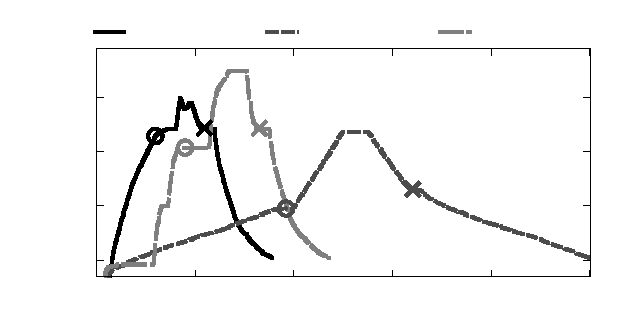
\includegraphics{RWCRuleForthnet}}%
    \gplfronttext
  \end{picture}%
\endgroup
}}
    \caption{\ourRouteUpdateName}
    \label{fig:rule_number:Forthnet:cu}
  \end{subfigure}
  \caption{Rules in the network during 178 path changes and
    accompanying NF migrations for Forthnet topology; markers show
    completion of path changes ($\times$) and NF migrations
    ({\LARGE $\circ$})}
\label{fig:rule_number:Forthnet}
\end{minipage}
\end{figure}
\fi

We measured the performance of our algorithm for NF migration and path
change, in comparison to other algorithms.  Each evaluation involved
$100$ runs, in which hosts sent $100$ packets per second for each
flow. \figref{fig:time} demonstrates the times required to finish both
NF migration and path changes; \figref{fig:time:fat} shows times for
100 path changes with two NF migrations per path change in a fat-tree
topology ($\portsPerSwitch = 8$), and \figref{fig:time:forthnet} shows
times for 178 path changes with three NF migrations per path change in
the Forthnet topology induced by breaking its ``busiest'' link
carrying the most flows.  Each boxplot in these figures represents 100
points, one per run; the box marks the first, second (median), and
third quartiles, and whiskers extend to cover points within
$1.5\times$ the interquartile range.  Outliers are shown as dots.


As can be seen in these figures, \sysname performed much faster than
SwingState and OpenNF, since NF migration and path change were
executed simultaneously. OpenNF required much more time to perform the
updates because it uses a single controller to buffer and redistribute
packets. Upon receiving a large number of incoming packets, the
controller consumed a lot of resources to process these packets, which
significantly slowed down the rule-update process.


\begin{figure}[H]
\centering
   \begin{subfigure}[b]{0.69\linewidth}
    \resizebox{\textwidth}{!}{\footnotesize{% GNUPLOT: LaTeX picture with Postscript
\begingroup
  \fontfamily{Times-Roman}%
  \selectfont
  \makeatletter
  \providecommand\color[2][]{%
    \GenericError{(gnuplot) \space\space\space\@spaces}{%
      Package color not loaded in conjunction with
      terminal option `colourtext'%
    }{See the gnuplot documentation for explanation.%
    }{Either use 'blacktext' in gnuplot or load the package
      color.sty in LaTeX.}%
    \renewcommand\color[2][]{}%
  }%
  \providecommand\includegraphics[2][]{%
    \GenericError{(gnuplot) \space\space\space\@spaces}{%
      Package graphicx or graphics not loaded%
    }{See the gnuplot documentation for explanation.%
    }{The gnuplot epslatex terminal needs graphicx.sty or graphics.sty.}%
    \renewcommand\includegraphics[2][]{}%
  }%
  \providecommand\rotatebox[2]{#2}%
  \@ifundefined{ifGPcolor}{%
    \newif\ifGPcolor
    \GPcolortrue
  }{}%
  \@ifundefined{ifGPblacktext}{%
    \newif\ifGPblacktext
    \GPblacktexttrue
  }{}%
  % define a \g@addto@macro without @ in the name:
  \let\gplgaddtomacro\g@addto@macro
  % define empty templates for all commands taking text:
  \gdef\gplbacktext{}%
  \gdef\gplfronttext{}%
  \makeatother
  \ifGPblacktext
    % no textcolor at all
    \def\colorrgb#1{}%
    \def\colorgray#1{}%
  \else
    % gray or color?
    \ifGPcolor
      \def\colorrgb#1{\color[rgb]{#1}}%
      \def\colorgray#1{\color[gray]{#1}}%
      \expandafter\def\csname LTw\endcsname{\color{white}}%
      \expandafter\def\csname LTb\endcsname{\color{black}}%
      \expandafter\def\csname LTa\endcsname{\color{black}}%
      \expandafter\def\csname LT0\endcsname{\color[rgb]{1,0,0}}%
      \expandafter\def\csname LT1\endcsname{\color[rgb]{0,1,0}}%
      \expandafter\def\csname LT2\endcsname{\color[rgb]{0,0,1}}%
      \expandafter\def\csname LT3\endcsname{\color[rgb]{1,0,1}}%
      \expandafter\def\csname LT4\endcsname{\color[rgb]{0,1,1}}%
      \expandafter\def\csname LT5\endcsname{\color[rgb]{1,1,0}}%
      \expandafter\def\csname LT6\endcsname{\color[rgb]{0,0,0}}%
      \expandafter\def\csname LT7\endcsname{\color[rgb]{1,0.3,0}}%
      \expandafter\def\csname LT8\endcsname{\color[rgb]{0.5,0.5,0.5}}%
    \else
      % gray
      \def\colorrgb#1{\color{black}}%
      \def\colorgray#1{\color[gray]{#1}}%
      \expandafter\def\csname LTw\endcsname{\color{white}}%
      \expandafter\def\csname LTb\endcsname{\color{black}}%
      \expandafter\def\csname LTa\endcsname{\color{black}}%
      \expandafter\def\csname LT0\endcsname{\color{black}}%
      \expandafter\def\csname LT1\endcsname{\color{black}}%
      \expandafter\def\csname LT2\endcsname{\color{black}}%
      \expandafter\def\csname LT3\endcsname{\color{black}}%
      \expandafter\def\csname LT4\endcsname{\color{black}}%
      \expandafter\def\csname LT5\endcsname{\color{black}}%
      \expandafter\def\csname LT6\endcsname{\color{black}}%
      \expandafter\def\csname LT7\endcsname{\color{black}}%
      \expandafter\def\csname LT8\endcsname{\color{black}}%
    \fi
  \fi
    \setlength{\unitlength}{0.0500bp}%
    \ifx\gptboxheight\undefined%
      \newlength{\gptboxheight}%
      \newlength{\gptboxwidth}%
      \newsavebox{\gptboxtext}%
    \fi%
    \setlength{\fboxrule}{0.5pt}%
    \setlength{\fboxsep}{1pt}%
\begin{picture}(5760.00,2880.00)%
    \gplgaddtomacro\gplbacktext{%
      \csname LTb\endcsname%%
      \put(686,554){\makebox(0,0)[r]{\strut{}$12250$}}%
      \put(686,1043){\makebox(0,0)[r]{\strut{}$12500$}}%
      \put(686,1532){\makebox(0,0)[r]{\strut{}$12750$}}%
      \put(686,2021){\makebox(0,0)[r]{\strut{}$13000$}}%
      \put(686,2510){\makebox(0,0)[r]{\strut{}$13250$}}%
      \put(770,252){\makebox(0,0){\strut{}$0$}}%
      \put(1260,252){\makebox(0,0){\strut{}$500$}}%
      \put(1750,252){\makebox(0,0){\strut{}$1000$}}%
      \put(2240,252){\makebox(0,0){\strut{}$1500$}}%
      \put(2730,252){\makebox(0,0){\strut{}$2000$}}%
      \put(3220,252){\makebox(0,0){\strut{}$2500$}}%
      \put(3710,252){\makebox(0,0){\strut{}$3000$}}%
      \put(4200,252){\makebox(0,0){\strut{}$3500$}}%
      \put(4690,252){\makebox(0,0){\strut{}$4000$}}%
      \put(5180,252){\makebox(0,0){\strut{}$4500$}}%
    }%
    \gplgaddtomacro\gplfronttext{%
      \csname LTb\endcsname%%
      \put(168,1474){\rotatebox{-270}{\makebox(0,0){\strut{}Total number of rules}}}%
      \put(3138,98){\makebox(0,0){\strut{}Time (ms)}}%
      \csname LTb\endcsname%%
      \put(1133,2733){\makebox(0,0)[l]{\strut{}SCC+Nimble}}%
      \csname LTb\endcsname%%
      \put(2792,2733){\makebox(0,0)[l]{\strut{}SCC+OpenNF}}%
      \csname LTb\endcsname%%
      \put(4451,2733){\makebox(0,0)[l]{\strut{}SCC+SwingState}}%
    }%
    \gplbacktext
    \put(0,0){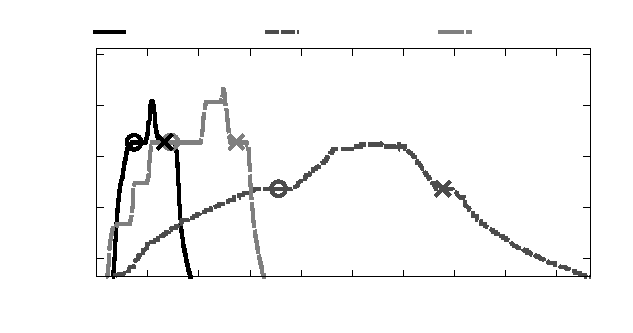
\includegraphics{SCCRuleFat}}%
    \gplfronttext
  \end{picture}%
\endgroup
}}
    \caption{SCC}
    \label{fig:rule_number:fat:scc}
  \end{subfigure}
  \par\bigskip
  \begin{subfigure}[b]{0.69\linewidth}
    \resizebox{\textwidth}{!}{\footnotesize{% GNUPLOT: LaTeX picture with Postscript
\begingroup
  \fontfamily{Times-Roman}%
  \selectfont
  \makeatletter
  \providecommand\color[2][]{%
    \GenericError{(gnuplot) \space\space\space\@spaces}{%
      Package color not loaded in conjunction with
      terminal option `colourtext'%
    }{See the gnuplot documentation for explanation.%
    }{Either use 'blacktext' in gnuplot or load the package
      color.sty in LaTeX.}%
    \renewcommand\color[2][]{}%
  }%
  \providecommand\includegraphics[2][]{%
    \GenericError{(gnuplot) \space\space\space\@spaces}{%
      Package graphicx or graphics not loaded%
    }{See the gnuplot documentation for explanation.%
    }{The gnuplot epslatex terminal needs graphicx.sty or graphics.sty.}%
    \renewcommand\includegraphics[2][]{}%
  }%
  \providecommand\rotatebox[2]{#2}%
  \@ifundefined{ifGPcolor}{%
    \newif\ifGPcolor
    \GPcolortrue
  }{}%
  \@ifundefined{ifGPblacktext}{%
    \newif\ifGPblacktext
    \GPblacktexttrue
  }{}%
  % define a \g@addto@macro without @ in the name:
  \let\gplgaddtomacro\g@addto@macro
  % define empty templates for all commands taking text:
  \gdef\gplbacktext{}%
  \gdef\gplfronttext{}%
  \makeatother
  \ifGPblacktext
    % no textcolor at all
    \def\colorrgb#1{}%
    \def\colorgray#1{}%
  \else
    % gray or color?
    \ifGPcolor
      \def\colorrgb#1{\color[rgb]{#1}}%
      \def\colorgray#1{\color[gray]{#1}}%
      \expandafter\def\csname LTw\endcsname{\color{white}}%
      \expandafter\def\csname LTb\endcsname{\color{black}}%
      \expandafter\def\csname LTa\endcsname{\color{black}}%
      \expandafter\def\csname LT0\endcsname{\color[rgb]{1,0,0}}%
      \expandafter\def\csname LT1\endcsname{\color[rgb]{0,1,0}}%
      \expandafter\def\csname LT2\endcsname{\color[rgb]{0,0,1}}%
      \expandafter\def\csname LT3\endcsname{\color[rgb]{1,0,1}}%
      \expandafter\def\csname LT4\endcsname{\color[rgb]{0,1,1}}%
      \expandafter\def\csname LT5\endcsname{\color[rgb]{1,1,0}}%
      \expandafter\def\csname LT6\endcsname{\color[rgb]{0,0,0}}%
      \expandafter\def\csname LT7\endcsname{\color[rgb]{1,0.3,0}}%
      \expandafter\def\csname LT8\endcsname{\color[rgb]{0.5,0.5,0.5}}%
    \else
      % gray
      \def\colorrgb#1{\color{black}}%
      \def\colorgray#1{\color[gray]{#1}}%
      \expandafter\def\csname LTw\endcsname{\color{white}}%
      \expandafter\def\csname LTb\endcsname{\color{black}}%
      \expandafter\def\csname LTa\endcsname{\color{black}}%
      \expandafter\def\csname LT0\endcsname{\color{black}}%
      \expandafter\def\csname LT1\endcsname{\color{black}}%
      \expandafter\def\csname LT2\endcsname{\color{black}}%
      \expandafter\def\csname LT3\endcsname{\color{black}}%
      \expandafter\def\csname LT4\endcsname{\color{black}}%
      \expandafter\def\csname LT5\endcsname{\color{black}}%
      \expandafter\def\csname LT6\endcsname{\color{black}}%
      \expandafter\def\csname LT7\endcsname{\color{black}}%
      \expandafter\def\csname LT8\endcsname{\color{black}}%
    \fi
  \fi
    \setlength{\unitlength}{0.0500bp}%
    \ifx\gptboxheight\undefined%
      \newlength{\gptboxheight}%
      \newlength{\gptboxwidth}%
      \newsavebox{\gptboxtext}%
    \fi%
    \setlength{\fboxrule}{0.5pt}%
    \setlength{\fboxsep}{1pt}%
\begin{picture}(5760.00,2880.00)%
    \gplgaddtomacro\gplbacktext{%
      \csname LTb\endcsname%%
      \put(686,588){\makebox(0,0)[r]{\strut{}$12300$}}%
      \put(686,1039){\makebox(0,0)[r]{\strut{}$12600$}}%
      \put(686,1490){\makebox(0,0)[r]{\strut{}$12900$}}%
      \put(686,1940){\makebox(0,0)[r]{\strut{}$13200$}}%
      \put(686,2391){\makebox(0,0)[r]{\strut{}$13500$}}%
      \put(770,252){\makebox(0,0){\strut{}$0$}}%
      \put(1557,252){\makebox(0,0){\strut{}$1000$}}%
      \put(2344,252){\makebox(0,0){\strut{}$2000$}}%
      \put(3130,252){\makebox(0,0){\strut{}$3000$}}%
      \put(3917,252){\makebox(0,0){\strut{}$4000$}}%
      \put(4704,252){\makebox(0,0){\strut{}$5000$}}%
      \put(5491,252){\makebox(0,0){\strut{}$6000$}}%
    }%
    \gplgaddtomacro\gplfronttext{%
      \csname LTb\endcsname%%
      \put(168,1474){\rotatebox{-270}{\makebox(0,0){\strut{}Total number of rules}}}%
      \put(3138,98){\makebox(0,0){\strut{}Time (ms)}}%
      \csname LTb\endcsname%%
      \put(1259,2733){\makebox(0,0)[l]{\strut{}CU+Nimble}}%
      \csname LTb\endcsname%%
      \put(2834,2733){\makebox(0,0)[l]{\strut{}CU+OpenNF}}%
      \csname LTb\endcsname%%
      \put(4409,2733){\makebox(0,0)[l]{\strut{}CU+SwingState}}%
    }%
    \gplbacktext
    \put(0,0){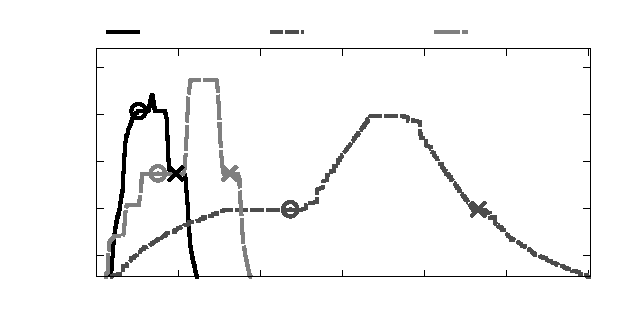
\includegraphics{CURuleFat}}%
    \gplfronttext
  \end{picture}%
\endgroup
}}
    \caption{CU}
    \label{fig:rule_number:fat:scc}
  \end{subfigure}
  \par\bigskip
  \begin{subfigure}[b]{0.69\linewidth}
    \resizebox{\textwidth}{!}{\footnotesize{% GNUPLOT: LaTeX picture with Postscript
\begingroup
  \fontfamily{Times-Roman}%
  \selectfont
  \makeatletter
  \providecommand\color[2][]{%
    \GenericError{(gnuplot) \space\space\space\@spaces}{%
      Package color not loaded in conjunction with
      terminal option `colourtext'%
    }{See the gnuplot documentation for explanation.%
    }{Either use 'blacktext' in gnuplot or load the package
      color.sty in LaTeX.}%
    \renewcommand\color[2][]{}%
  }%
  \providecommand\includegraphics[2][]{%
    \GenericError{(gnuplot) \space\space\space\@spaces}{%
      Package graphicx or graphics not loaded%
    }{See the gnuplot documentation for explanation.%
    }{The gnuplot epslatex terminal needs graphicx.sty or graphics.sty.}%
    \renewcommand\includegraphics[2][]{}%
  }%
  \providecommand\rotatebox[2]{#2}%
  \@ifundefined{ifGPcolor}{%
    \newif\ifGPcolor
    \GPcolortrue
  }{}%
  \@ifundefined{ifGPblacktext}{%
    \newif\ifGPblacktext
    \GPblacktexttrue
  }{}%
  % define a \g@addto@macro without @ in the name:
  \let\gplgaddtomacro\g@addto@macro
  % define empty templates for all commands taking text:
  \gdef\gplbacktext{}%
  \gdef\gplfronttext{}%
  \makeatother
  \ifGPblacktext
    % no textcolor at all
    \def\colorrgb#1{}%
    \def\colorgray#1{}%
  \else
    % gray or color?
    \ifGPcolor
      \def\colorrgb#1{\color[rgb]{#1}}%
      \def\colorgray#1{\color[gray]{#1}}%
      \expandafter\def\csname LTw\endcsname{\color{white}}%
      \expandafter\def\csname LTb\endcsname{\color{black}}%
      \expandafter\def\csname LTa\endcsname{\color{black}}%
      \expandafter\def\csname LT0\endcsname{\color[rgb]{1,0,0}}%
      \expandafter\def\csname LT1\endcsname{\color[rgb]{0,1,0}}%
      \expandafter\def\csname LT2\endcsname{\color[rgb]{0,0,1}}%
      \expandafter\def\csname LT3\endcsname{\color[rgb]{1,0,1}}%
      \expandafter\def\csname LT4\endcsname{\color[rgb]{0,1,1}}%
      \expandafter\def\csname LT5\endcsname{\color[rgb]{1,1,0}}%
      \expandafter\def\csname LT6\endcsname{\color[rgb]{0,0,0}}%
      \expandafter\def\csname LT7\endcsname{\color[rgb]{1,0.3,0}}%
      \expandafter\def\csname LT8\endcsname{\color[rgb]{0.5,0.5,0.5}}%
    \else
      % gray
      \def\colorrgb#1{\color{black}}%
      \def\colorgray#1{\color[gray]{#1}}%
      \expandafter\def\csname LTw\endcsname{\color{white}}%
      \expandafter\def\csname LTb\endcsname{\color{black}}%
      \expandafter\def\csname LTa\endcsname{\color{black}}%
      \expandafter\def\csname LT0\endcsname{\color{black}}%
      \expandafter\def\csname LT1\endcsname{\color{black}}%
      \expandafter\def\csname LT2\endcsname{\color{black}}%
      \expandafter\def\csname LT3\endcsname{\color{black}}%
      \expandafter\def\csname LT4\endcsname{\color{black}}%
      \expandafter\def\csname LT5\endcsname{\color{black}}%
      \expandafter\def\csname LT6\endcsname{\color{black}}%
      \expandafter\def\csname LT7\endcsname{\color{black}}%
      \expandafter\def\csname LT8\endcsname{\color{black}}%
    \fi
  \fi
    \setlength{\unitlength}{0.0500bp}%
    \ifx\gptboxheight\undefined%
      \newlength{\gptboxheight}%
      \newlength{\gptboxwidth}%
      \newsavebox{\gptboxtext}%
    \fi%
    \setlength{\fboxrule}{0.5pt}%
    \setlength{\fboxsep}{1pt}%
\begin{picture}(5760.00,2880.00)%
    \gplgaddtomacro\gplbacktext{%
      \csname LTb\endcsname%%
      \put(686,547){\makebox(0,0)[r]{\strut{}$12250$}}%
      \put(686,1015){\makebox(0,0)[r]{\strut{}$12500$}}%
      \put(686,1484){\makebox(0,0)[r]{\strut{}$12750$}}%
      \put(686,1952){\makebox(0,0)[r]{\strut{}$13000$}}%
      \put(686,2421){\makebox(0,0)[r]{\strut{}$13250$}}%
      \put(770,252){\makebox(0,0){\strut{}$0$}}%
      \put(1272,252){\makebox(0,0){\strut{}$500$}}%
      \put(1775,252){\makebox(0,0){\strut{}$1000$}}%
      \put(2277,252){\makebox(0,0){\strut{}$1500$}}%
      \put(2780,252){\makebox(0,0){\strut{}$2000$}}%
      \put(3282,252){\makebox(0,0){\strut{}$2500$}}%
      \put(3785,252){\makebox(0,0){\strut{}$3000$}}%
      \put(4287,252){\makebox(0,0){\strut{}$3500$}}%
      \put(4790,252){\makebox(0,0){\strut{}$4000$}}%
      \put(5292,252){\makebox(0,0){\strut{}$4500$}}%
    }%
    \gplgaddtomacro\gplfronttext{%
      \csname LTb\endcsname%%
      \put(168,1474){\rotatebox{-270}{\makebox(0,0){\strut{}Total number of rules}}}%
      \put(3138,98){\makebox(0,0){\strut{}Time (ms)}}%
      \csname LTb\endcsname%%
      \put(1133,2733){\makebox(0,0)[l]{\strut{}RWC+Nimble}}%
      \csname LTb\endcsname%%
      \put(2792,2733){\makebox(0,0)[l]{\strut{}RWC+OpenNF}}%
      \csname LTb\endcsname%%
      \put(4451,2733){\makebox(0,0)[l]{\strut{}RWC+SwingState}}%
    }%
    \gplbacktext
    \put(0,0){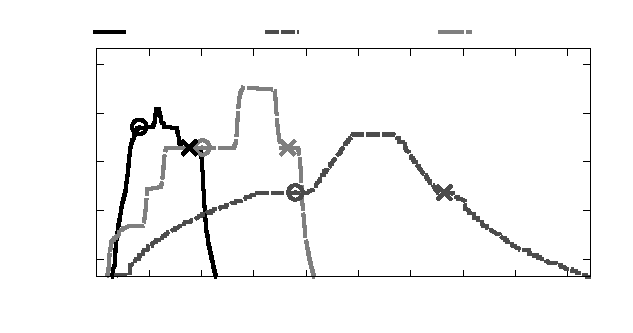
\includegraphics{RWCRuleFat}}%
    \gplfronttext
  \end{picture}%
\endgroup
}}
    \caption{\ourRouteUpdateName}
    \label{fig:rule_number:fat:cu}
  \end{subfigure}
  \caption{Rules in the network during 100 path changes and
    accompanying NF migrations for fat-tree topology; markers show
    completion of path changes ($\times$) and NF migrations
    ({\LARGE $\circ$})}
\label{fig:rule_number:fat}
\end{figure}



\subsection{Memory Overhead in Switches}


To evaluate the number of rules (including rules to build tunnels)
imposed on the switches by each algorithm, we examined the per-switch
logs of rule installations and deletions over 100 consecutive path
changes in the fat-tree topology ($\portsPerSwitch = 8$). We computed
a time series of the total number of rules installed across all
switches in the network, including the time cleaning up tunnels used
to migrate NFs and to tunnel traffic. This time series for a
representative run of each of SCC, CU, and \ourRouteUpdateName using
\sysname, SwingState and OpenNF is shown in
\figref{fig:rule_number:fat}.  We repeated this evaluation on the
Forthnet topology, but by breaking the busiest link; see
\figref{fig:rule_number:Forthnet}.  Each curve is marked with the time
when NF migration for all flows was done and the time when all path
changes were completed.  All three algorithms require installing rules
on \oldSwitchID{\nfIdx} and \newSwitchID{\nfIdx} to deal with incoming
packets and also to clean up these rules.  Different from OpenNF,
\sysname and SwingState need to build tunnels to migrate NFs and to
tunnel traffic.  As these figures show, \sysname requires less time to
finish NF migrations and path changes, because it performs both
operations simultaneously. OpenNF needs more time to finish path changes
than SwingState since OpenNF buffers and redistributes all incoming packets in the controller,
which induces a large delay before path change can be executed.


\begin{figure}[H]
\centering
   \begin{subfigure}[b]{0.69\linewidth}
    \resizebox{\textwidth}{!}{\footnotesize{% GNUPLOT: LaTeX picture with Postscript
\begingroup
  \fontfamily{Times-Roman}%
  \selectfont
  \makeatletter
  \providecommand\color[2][]{%
    \GenericError{(gnuplot) \space\space\space\@spaces}{%
      Package color not loaded in conjunction with
      terminal option `colourtext'%
    }{See the gnuplot documentation for explanation.%
    }{Either use 'blacktext' in gnuplot or load the package
      color.sty in LaTeX.}%
    \renewcommand\color[2][]{}%
  }%
  \providecommand\includegraphics[2][]{%
    \GenericError{(gnuplot) \space\space\space\@spaces}{%
      Package graphicx or graphics not loaded%
    }{See the gnuplot documentation for explanation.%
    }{The gnuplot epslatex terminal needs graphicx.sty or graphics.sty.}%
    \renewcommand\includegraphics[2][]{}%
  }%
  \providecommand\rotatebox[2]{#2}%
  \@ifundefined{ifGPcolor}{%
    \newif\ifGPcolor
    \GPcolortrue
  }{}%
  \@ifundefined{ifGPblacktext}{%
    \newif\ifGPblacktext
    \GPblacktexttrue
  }{}%
  % define a \g@addto@macro without @ in the name:
  \let\gplgaddtomacro\g@addto@macro
  % define empty templates for all commands taking text:
  \gdef\gplbacktext{}%
  \gdef\gplfronttext{}%
  \makeatother
  \ifGPblacktext
    % no textcolor at all
    \def\colorrgb#1{}%
    \def\colorgray#1{}%
  \else
    % gray or color?
    \ifGPcolor
      \def\colorrgb#1{\color[rgb]{#1}}%
      \def\colorgray#1{\color[gray]{#1}}%
      \expandafter\def\csname LTw\endcsname{\color{white}}%
      \expandafter\def\csname LTb\endcsname{\color{black}}%
      \expandafter\def\csname LTa\endcsname{\color{black}}%
      \expandafter\def\csname LT0\endcsname{\color[rgb]{1,0,0}}%
      \expandafter\def\csname LT1\endcsname{\color[rgb]{0,1,0}}%
      \expandafter\def\csname LT2\endcsname{\color[rgb]{0,0,1}}%
      \expandafter\def\csname LT3\endcsname{\color[rgb]{1,0,1}}%
      \expandafter\def\csname LT4\endcsname{\color[rgb]{0,1,1}}%
      \expandafter\def\csname LT5\endcsname{\color[rgb]{1,1,0}}%
      \expandafter\def\csname LT6\endcsname{\color[rgb]{0,0,0}}%
      \expandafter\def\csname LT7\endcsname{\color[rgb]{1,0.3,0}}%
      \expandafter\def\csname LT8\endcsname{\color[rgb]{0.5,0.5,0.5}}%
    \else
      % gray
      \def\colorrgb#1{\color{black}}%
      \def\colorgray#1{\color[gray]{#1}}%
      \expandafter\def\csname LTw\endcsname{\color{white}}%
      \expandafter\def\csname LTb\endcsname{\color{black}}%
      \expandafter\def\csname LTa\endcsname{\color{black}}%
      \expandafter\def\csname LT0\endcsname{\color{black}}%
      \expandafter\def\csname LT1\endcsname{\color{black}}%
      \expandafter\def\csname LT2\endcsname{\color{black}}%
      \expandafter\def\csname LT3\endcsname{\color{black}}%
      \expandafter\def\csname LT4\endcsname{\color{black}}%
      \expandafter\def\csname LT5\endcsname{\color{black}}%
      \expandafter\def\csname LT6\endcsname{\color{black}}%
      \expandafter\def\csname LT7\endcsname{\color{black}}%
      \expandafter\def\csname LT8\endcsname{\color{black}}%
    \fi
  \fi
    \setlength{\unitlength}{0.0500bp}%
    \ifx\gptboxheight\undefined%
      \newlength{\gptboxheight}%
      \newlength{\gptboxwidth}%
      \newsavebox{\gptboxtext}%
    \fi%
    \setlength{\fboxrule}{0.5pt}%
    \setlength{\fboxsep}{1pt}%
\begin{picture}(5760.00,2880.00)%
    \gplgaddtomacro\gplbacktext{%
      \csname LTb\endcsname%%
      \put(686,553){\makebox(0,0)[r]{\strut{}$12000$}}%
      \put(686,1005){\makebox(0,0)[r]{\strut{}$12400$}}%
      \put(686,1456){\makebox(0,0)[r]{\strut{}$12800$}}%
      \put(686,1908){\makebox(0,0)[r]{\strut{}$13200$}}%
      \put(686,2360){\makebox(0,0)[r]{\strut{}$13600$}}%
      \put(770,252){\makebox(0,0){\strut{}$0$}}%
      \put(1627,252){\makebox(0,0){\strut{}$2000$}}%
      \put(2483,252){\makebox(0,0){\strut{}$4000$}}%
      \put(3340,252){\makebox(0,0){\strut{}$6000$}}%
      \put(4197,252){\makebox(0,0){\strut{}$8000$}}%
      \put(5053,252){\makebox(0,0){\strut{}$10000$}}%
    }%
    \gplgaddtomacro\gplfronttext{%
      \csname LTb\endcsname%%
      \put(168,1474){\rotatebox{-270}{\makebox(0,0){\strut{}Total number of rules}}}%
      \put(3138,98){\makebox(0,0){\strut{}Time (ms)}}%
      \csname LTb\endcsname%%
      \put(1133,2733){\makebox(0,0)[l]{\strut{}SCC+Nimble}}%
      \csname LTb\endcsname%%
      \put(2792,2733){\makebox(0,0)[l]{\strut{}SCC+OpenNF}}%
      \csname LTb\endcsname%%
      \put(4451,2733){\makebox(0,0)[l]{\strut{}SCC+SwingState}}%
    }%
    \gplbacktext
    \put(0,0){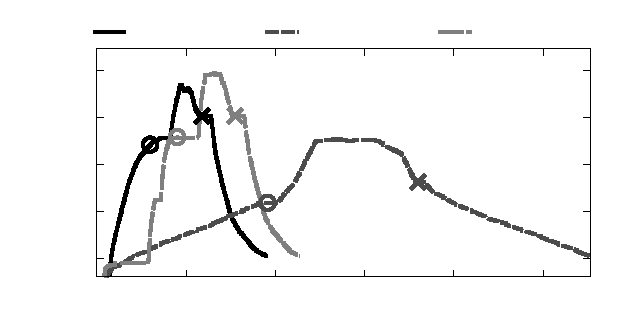
\includegraphics{SCCRuleForthnet}}%
    \gplfronttext
  \end{picture}%
\endgroup
}}
    \caption{SCC}
    \label{fig:rule_number:Forthnet:scc}
  \end{subfigure}
  \par\bigskip
  \begin{subfigure}[b]{0.69\linewidth}
    \resizebox{\textwidth}{!}{\footnotesize{% GNUPLOT: LaTeX picture with Postscript
\begingroup
  \fontfamily{Times-Roman}%
  \selectfont
  \makeatletter
  \providecommand\color[2][]{%
    \GenericError{(gnuplot) \space\space\space\@spaces}{%
      Package color not loaded in conjunction with
      terminal option `colourtext'%
    }{See the gnuplot documentation for explanation.%
    }{Either use 'blacktext' in gnuplot or load the package
      color.sty in LaTeX.}%
    \renewcommand\color[2][]{}%
  }%
  \providecommand\includegraphics[2][]{%
    \GenericError{(gnuplot) \space\space\space\@spaces}{%
      Package graphicx or graphics not loaded%
    }{See the gnuplot documentation for explanation.%
    }{The gnuplot epslatex terminal needs graphicx.sty or graphics.sty.}%
    \renewcommand\includegraphics[2][]{}%
  }%
  \providecommand\rotatebox[2]{#2}%
  \@ifundefined{ifGPcolor}{%
    \newif\ifGPcolor
    \GPcolortrue
  }{}%
  \@ifundefined{ifGPblacktext}{%
    \newif\ifGPblacktext
    \GPblacktexttrue
  }{}%
  % define a \g@addto@macro without @ in the name:
  \let\gplgaddtomacro\g@addto@macro
  % define empty templates for all commands taking text:
  \gdef\gplbacktext{}%
  \gdef\gplfronttext{}%
  \makeatother
  \ifGPblacktext
    % no textcolor at all
    \def\colorrgb#1{}%
    \def\colorgray#1{}%
  \else
    % gray or color?
    \ifGPcolor
      \def\colorrgb#1{\color[rgb]{#1}}%
      \def\colorgray#1{\color[gray]{#1}}%
      \expandafter\def\csname LTw\endcsname{\color{white}}%
      \expandafter\def\csname LTb\endcsname{\color{black}}%
      \expandafter\def\csname LTa\endcsname{\color{black}}%
      \expandafter\def\csname LT0\endcsname{\color[rgb]{1,0,0}}%
      \expandafter\def\csname LT1\endcsname{\color[rgb]{0,1,0}}%
      \expandafter\def\csname LT2\endcsname{\color[rgb]{0,0,1}}%
      \expandafter\def\csname LT3\endcsname{\color[rgb]{1,0,1}}%
      \expandafter\def\csname LT4\endcsname{\color[rgb]{0,1,1}}%
      \expandafter\def\csname LT5\endcsname{\color[rgb]{1,1,0}}%
      \expandafter\def\csname LT6\endcsname{\color[rgb]{0,0,0}}%
      \expandafter\def\csname LT7\endcsname{\color[rgb]{1,0.3,0}}%
      \expandafter\def\csname LT8\endcsname{\color[rgb]{0.5,0.5,0.5}}%
    \else
      % gray
      \def\colorrgb#1{\color{black}}%
      \def\colorgray#1{\color[gray]{#1}}%
      \expandafter\def\csname LTw\endcsname{\color{white}}%
      \expandafter\def\csname LTb\endcsname{\color{black}}%
      \expandafter\def\csname LTa\endcsname{\color{black}}%
      \expandafter\def\csname LT0\endcsname{\color{black}}%
      \expandafter\def\csname LT1\endcsname{\color{black}}%
      \expandafter\def\csname LT2\endcsname{\color{black}}%
      \expandafter\def\csname LT3\endcsname{\color{black}}%
      \expandafter\def\csname LT4\endcsname{\color{black}}%
      \expandafter\def\csname LT5\endcsname{\color{black}}%
      \expandafter\def\csname LT6\endcsname{\color{black}}%
      \expandafter\def\csname LT7\endcsname{\color{black}}%
      \expandafter\def\csname LT8\endcsname{\color{black}}%
    \fi
  \fi
    \setlength{\unitlength}{0.0500bp}%
    \ifx\gptboxheight\undefined%
      \newlength{\gptboxheight}%
      \newlength{\gptboxwidth}%
      \newsavebox{\gptboxtext}%
    \fi%
    \setlength{\fboxrule}{0.5pt}%
    \setlength{\fboxsep}{1pt}%
\begin{picture}(5760.00,2880.00)%
    \gplgaddtomacro\gplbacktext{%
      \csname LTb\endcsname%%
      \put(686,417){\makebox(0,0)[r]{\strut{}$11900$}}%
      \put(686,920){\makebox(0,0)[r]{\strut{}$12600$}}%
      \put(686,1422){\makebox(0,0)[r]{\strut{}$13300$}}%
      \put(686,1924){\makebox(0,0)[r]{\strut{}$14000$}}%
      \put(686,2427){\makebox(0,0)[r]{\strut{}$14700$}}%
      \put(770,252){\makebox(0,0){\strut{}$0$}}%
      \put(1509,252){\makebox(0,0){\strut{}$2000$}}%
      \put(2248,252){\makebox(0,0){\strut{}$4000$}}%
      \put(2986,252){\makebox(0,0){\strut{}$6000$}}%
      \put(3725,252){\makebox(0,0){\strut{}$8000$}}%
      \put(4464,252){\makebox(0,0){\strut{}$10000$}}%
      \put(5203,252){\makebox(0,0){\strut{}$12000$}}%
    }%
    \gplgaddtomacro\gplfronttext{%
      \csname LTb\endcsname%%
      \put(168,1474){\rotatebox{-270}{\makebox(0,0){\strut{}Total number of rules}}}%
      \put(3138,98){\makebox(0,0){\strut{}Time (ms)}}%
      \csname LTb\endcsname%%
      \put(1259,2733){\makebox(0,0)[l]{\strut{}CU+Nimble}}%
      \csname LTb\endcsname%%
      \put(2834,2733){\makebox(0,0)[l]{\strut{}CU+OpenNF}}%
      \csname LTb\endcsname%%
      \put(4409,2733){\makebox(0,0)[l]{\strut{}CU+SwingState}}%
    }%
    \gplbacktext
    \put(0,0){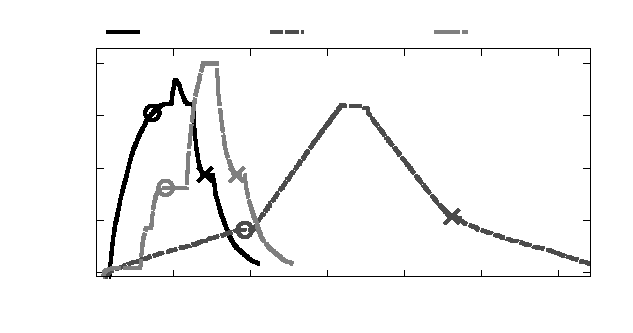
\includegraphics{CURuleForthnet}}%
    \gplfronttext
  \end{picture}%
\endgroup
}}
    \caption{CU}
    \label{fig:rule_number:Forthnet:scc}
  \end{subfigure}
  \par\bigskip
  \begin{subfigure}[b]{0.69\linewidth}
    \resizebox{\textwidth}{!}{\small{% GNUPLOT: LaTeX picture with Postscript
\begingroup
  \fontfamily{Times-Roman}%
  \selectfont
  \makeatletter
  \providecommand\color[2][]{%
    \GenericError{(gnuplot) \space\space\space\@spaces}{%
      Package color not loaded in conjunction with
      terminal option `colourtext'%
    }{See the gnuplot documentation for explanation.%
    }{Either use 'blacktext' in gnuplot or load the package
      color.sty in LaTeX.}%
    \renewcommand\color[2][]{}%
  }%
  \providecommand\includegraphics[2][]{%
    \GenericError{(gnuplot) \space\space\space\@spaces}{%
      Package graphicx or graphics not loaded%
    }{See the gnuplot documentation for explanation.%
    }{The gnuplot epslatex terminal needs graphicx.sty or graphics.sty.}%
    \renewcommand\includegraphics[2][]{}%
  }%
  \providecommand\rotatebox[2]{#2}%
  \@ifundefined{ifGPcolor}{%
    \newif\ifGPcolor
    \GPcolortrue
  }{}%
  \@ifundefined{ifGPblacktext}{%
    \newif\ifGPblacktext
    \GPblacktexttrue
  }{}%
  % define a \g@addto@macro without @ in the name:
  \let\gplgaddtomacro\g@addto@macro
  % define empty templates for all commands taking text:
  \gdef\gplbacktext{}%
  \gdef\gplfronttext{}%
  \makeatother
  \ifGPblacktext
    % no textcolor at all
    \def\colorrgb#1{}%
    \def\colorgray#1{}%
  \else
    % gray or color?
    \ifGPcolor
      \def\colorrgb#1{\color[rgb]{#1}}%
      \def\colorgray#1{\color[gray]{#1}}%
      \expandafter\def\csname LTw\endcsname{\color{white}}%
      \expandafter\def\csname LTb\endcsname{\color{black}}%
      \expandafter\def\csname LTa\endcsname{\color{black}}%
      \expandafter\def\csname LT0\endcsname{\color[rgb]{1,0,0}}%
      \expandafter\def\csname LT1\endcsname{\color[rgb]{0,1,0}}%
      \expandafter\def\csname LT2\endcsname{\color[rgb]{0,0,1}}%
      \expandafter\def\csname LT3\endcsname{\color[rgb]{1,0,1}}%
      \expandafter\def\csname LT4\endcsname{\color[rgb]{0,1,1}}%
      \expandafter\def\csname LT5\endcsname{\color[rgb]{1,1,0}}%
      \expandafter\def\csname LT6\endcsname{\color[rgb]{0,0,0}}%
      \expandafter\def\csname LT7\endcsname{\color[rgb]{1,0.3,0}}%
      \expandafter\def\csname LT8\endcsname{\color[rgb]{0.5,0.5,0.5}}%
    \else
      % gray
      \def\colorrgb#1{\color{black}}%
      \def\colorgray#1{\color[gray]{#1}}%
      \expandafter\def\csname LTw\endcsname{\color{white}}%
      \expandafter\def\csname LTb\endcsname{\color{black}}%
      \expandafter\def\csname LTa\endcsname{\color{black}}%
      \expandafter\def\csname LT0\endcsname{\color{black}}%
      \expandafter\def\csname LT1\endcsname{\color{black}}%
      \expandafter\def\csname LT2\endcsname{\color{black}}%
      \expandafter\def\csname LT3\endcsname{\color{black}}%
      \expandafter\def\csname LT4\endcsname{\color{black}}%
      \expandafter\def\csname LT5\endcsname{\color{black}}%
      \expandafter\def\csname LT6\endcsname{\color{black}}%
      \expandafter\def\csname LT7\endcsname{\color{black}}%
      \expandafter\def\csname LT8\endcsname{\color{black}}%
    \fi
  \fi
    \setlength{\unitlength}{0.0500bp}%
    \ifx\gptboxheight\undefined%
      \newlength{\gptboxheight}%
      \newlength{\gptboxwidth}%
      \newsavebox{\gptboxtext}%
    \fi%
    \setlength{\fboxrule}{0.5pt}%
    \setlength{\fboxsep}{1pt}%
\begin{picture}(5760.00,2880.00)%
    \gplgaddtomacro\gplbacktext{%
      \csname LTb\endcsname%%
      \put(686,540){\makebox(0,0)[r]{\strut{}$12000$}}%
      \put(686,1061){\makebox(0,0)[r]{\strut{}$12500$}}%
      \put(686,1582){\makebox(0,0)[r]{\strut{}$13000$}}%
      \put(686,2104){\makebox(0,0)[r]{\strut{}$13500$}}%
      \put(770,252){\makebox(0,0){\strut{}$0$}}%
      \put(1716,252){\makebox(0,0){\strut{}$2000$}}%
      \put(2662,252){\makebox(0,0){\strut{}$4000$}}%
      \put(3608,252){\makebox(0,0){\strut{}$6000$}}%
      \put(4554,252){\makebox(0,0){\strut{}$8000$}}%
      \put(5500,252){\makebox(0,0){\strut{}$10000$}}%
    }%
    \gplgaddtomacro\gplfronttext{%
      \csname LTb\endcsname%%
      \put(168,1474){\rotatebox{-270}{\makebox(0,0){\strut{}Total number of rules}}}%
      \put(3138,98){\makebox(0,0){\strut{}Time (ms)}}%
      \csname LTb\endcsname%%
      \put(1133,2733){\makebox(0,0)[l]{\strut{}RWC+Nimble}}%
      \csname LTb\endcsname%%
      \put(2792,2733){\makebox(0,0)[l]{\strut{}RWC+OpenNF}}%
      \csname LTb\endcsname%%
      \put(4451,2733){\makebox(0,0)[l]{\strut{}RWC+SwingState}}%
    }%
    \gplbacktext
    \put(0,0){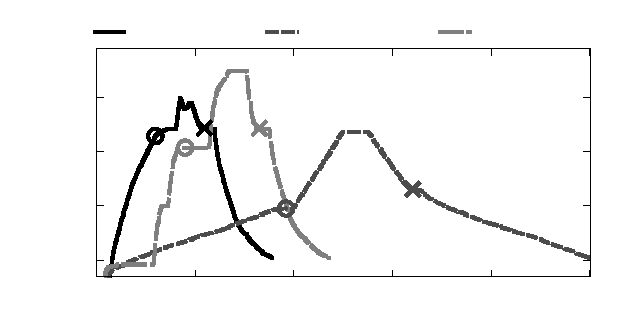
\includegraphics{RWCRuleForthnet}}%
    \gplfronttext
  \end{picture}%
\endgroup
}}
    \caption{\ourRouteUpdateName}
    \label{fig:rule_number:Forthnet:cu}
  \end{subfigure}
  \caption{Rules in the network during 178 path changes and
    accompanying NF migrations for Forthnet topology; markers show
    completion of path changes ($\times$) and NF migrations
    ({\LARGE $\circ$})}
\label{fig:rule_number:Forthnet}
\end{figure}



\subsection{Packet Latency During Link Failure}

To evaluate the latency imposed on each flow upon link failure by each
algorithm, we measured the time required for a destination host to
receive $10\megabytes$ from a source host through a TCP connection. We
broke one random link and selected $10$ flows to update their routing
polices.  The source host of each flow started to send a stream of
packets at speed $100\megabits/\sec$ to the destination host upon link
failure. The time shown in \figref{fig:latency} shows the times for
the destination to receive $10\megabytes$ using each
algorithm. \sysname outperforms SwingState and OpenNF because \sysname
recovers the new path more efficiently by performing NF migration and
path update simultaneously.  Though SwingState also uses tunnels to
migrate NFs, it mirrors packets but still delivers packets through
the old path during NF migration.  Plus, OpenNF uses a single
controller to redistribute incoming packets, which significantly slows
down the speed.

\begin{figure}[t]
\centering
 \begin{subfigure}[b]{0.7\columnwidth}
    \resizebox{\textwidth}{!}{\footnotesize{% GNUPLOT: LaTeX picture with Postscript
\begingroup
  \fontfamily{Times-Roman}%
  \selectfont
  \makeatletter
  \providecommand\color[2][]{%
    \GenericError{(gnuplot) \space\space\space\@spaces}{%
      Package color not loaded in conjunction with
      terminal option `colourtext'%
    }{See the gnuplot documentation for explanation.%
    }{Either use 'blacktext' in gnuplot or load the package
      color.sty in LaTeX.}%
    \renewcommand\color[2][]{}%
  }%
  \providecommand\includegraphics[2][]{%
    \GenericError{(gnuplot) \space\space\space\@spaces}{%
      Package graphicx or graphics not loaded%
    }{See the gnuplot documentation for explanation.%
    }{The gnuplot epslatex terminal needs graphicx.sty or graphics.sty.}%
    \renewcommand\includegraphics[2][]{}%
  }%
  \providecommand\rotatebox[2]{#2}%
  \@ifundefined{ifGPcolor}{%
    \newif\ifGPcolor
    \GPcolortrue
  }{}%
  \@ifundefined{ifGPblacktext}{%
    \newif\ifGPblacktext
    \GPblacktexttrue
  }{}%
  % define a \g@addto@macro without @ in the name:
  \let\gplgaddtomacro\g@addto@macro
  % define empty templates for all commands taking text:
  \gdef\gplbacktext{}%
  \gdef\gplfronttext{}%
  \makeatother
  \ifGPblacktext
    % no textcolor at all
    \def\colorrgb#1{}%
    \def\colorgray#1{}%
  \else
    % gray or color?
    \ifGPcolor
      \def\colorrgb#1{\color[rgb]{#1}}%
      \def\colorgray#1{\color[gray]{#1}}%
      \expandafter\def\csname LTw\endcsname{\color{white}}%
      \expandafter\def\csname LTb\endcsname{\color{black}}%
      \expandafter\def\csname LTa\endcsname{\color{black}}%
      \expandafter\def\csname LT0\endcsname{\color[rgb]{1,0,0}}%
      \expandafter\def\csname LT1\endcsname{\color[rgb]{0,1,0}}%
      \expandafter\def\csname LT2\endcsname{\color[rgb]{0,0,1}}%
      \expandafter\def\csname LT3\endcsname{\color[rgb]{1,0,1}}%
      \expandafter\def\csname LT4\endcsname{\color[rgb]{0,1,1}}%
      \expandafter\def\csname LT5\endcsname{\color[rgb]{1,1,0}}%
      \expandafter\def\csname LT6\endcsname{\color[rgb]{0,0,0}}%
      \expandafter\def\csname LT7\endcsname{\color[rgb]{1,0.3,0}}%
      \expandafter\def\csname LT8\endcsname{\color[rgb]{0.5,0.5,0.5}}%
    \else
      % gray
      \def\colorrgb#1{\color{black}}%
      \def\colorgray#1{\color[gray]{#1}}%
      \expandafter\def\csname LTw\endcsname{\color{white}}%
      \expandafter\def\csname LTb\endcsname{\color{black}}%
      \expandafter\def\csname LTa\endcsname{\color{black}}%
      \expandafter\def\csname LT0\endcsname{\color{black}}%
      \expandafter\def\csname LT1\endcsname{\color{black}}%
      \expandafter\def\csname LT2\endcsname{\color{black}}%
      \expandafter\def\csname LT3\endcsname{\color{black}}%
      \expandafter\def\csname LT4\endcsname{\color{black}}%
      \expandafter\def\csname LT5\endcsname{\color{black}}%
      \expandafter\def\csname LT6\endcsname{\color{black}}%
      \expandafter\def\csname LT7\endcsname{\color{black}}%
      \expandafter\def\csname LT8\endcsname{\color{black}}%
    \fi
  \fi
    \setlength{\unitlength}{0.0500bp}%
    \ifx\gptboxheight\undefined%
      \newlength{\gptboxheight}%
      \newlength{\gptboxwidth}%
      \newsavebox{\gptboxtext}%
    \fi%
    \setlength{\fboxrule}{0.5pt}%
    \setlength{\fboxsep}{1pt}%
\begin{picture}(7200.00,2880.00)%
    \gplgaddtomacro\gplbacktext{%
      \csname LTb\endcsname%%
      \put(782,528){\makebox(0,0)[r]{\strut{}$1100$}}%
      \csname LTb\endcsname%%
      \put(782,1089){\makebox(0,0)[r]{\strut{}$1110$}}%
      \csname LTb\endcsname%%
      \put(782,1651){\makebox(0,0)[r]{\strut{}$1120$}}%
      \csname LTb\endcsname%%
      \put(782,2212){\makebox(0,0)[r]{\strut{}$1130$}}%
      \csname LTb\endcsname%%
      \put(1126,242){\rotatebox{25}{\makebox(0,0)[r]{\strut{}SCC}}}%
      \csname LTb\endcsname%%
      \put(1617,242){\rotatebox{25}{\makebox(0,0)[r]{\strut{}CU}}}%
      \csname LTb\endcsname%%
      \put(2107,242){\rotatebox{25}{\makebox(0,0)[r]{\strut{}RWC}}}%
    }%
    \gplgaddtomacro\gplfronttext{%
      \csname LTb\endcsname%%
      \put(137,1482){\rotatebox{-270}{\makebox(0,0){\strut{}Time (ms)}}}%
      \csname LTb\endcsname%%
      \put(1439,2701){\makebox(0,0){\strut{}Nimble}}%
    }%
    \gplgaddtomacro\gplbacktext{%
      \csname LTb\endcsname%%
      \put(2942,528){\makebox(0,0)[r]{\strut{}$2330$}}%
      \csname LTb\endcsname%%
      \put(2942,1089){\makebox(0,0)[r]{\strut{}$2338$}}%
      \csname LTb\endcsname%%
      \put(2942,1651){\makebox(0,0)[r]{\strut{}$2346$}}%
      \csname LTb\endcsname%%
      \put(2942,2212){\makebox(0,0)[r]{\strut{}$2354$}}%
      \csname LTb\endcsname%%
      \put(3286,242){\rotatebox{25}{\makebox(0,0)[r]{\strut{}SCC}}}%
      \csname LTb\endcsname%%
      \put(3777,242){\rotatebox{25}{\makebox(0,0)[r]{\strut{}CU}}}%
      \csname LTb\endcsname%%
      \put(4267,242){\rotatebox{25}{\makebox(0,0)[r]{\strut{}RWC}}}%
    }%
    \gplgaddtomacro\gplfronttext{%
      \csname LTb\endcsname%%
      \put(3599,2701){\makebox(0,0){\strut{}SwingState}}%
    }%
    \gplgaddtomacro\gplbacktext{%
      \csname LTb\endcsname%%
      \put(5102,528){\makebox(0,0)[r]{\strut{}$1520$}}%
      \csname LTb\endcsname%%
      \put(5102,1089){\makebox(0,0)[r]{\strut{}$1526$}}%
      \csname LTb\endcsname%%
      \put(5102,1651){\makebox(0,0)[r]{\strut{}$1532$}}%
      \csname LTb\endcsname%%
      \put(5102,2212){\makebox(0,0)[r]{\strut{}$1538$}}%
      \csname LTb\endcsname%%
      \put(5446,242){\rotatebox{25}{\makebox(0,0)[r]{\strut{}SCC}}}%
      \csname LTb\endcsname%%
      \put(5937,242){\rotatebox{25}{\makebox(0,0)[r]{\strut{}CU}}}%
      \csname LTb\endcsname%%
      \put(6427,242){\rotatebox{25}{\makebox(0,0)[r]{\strut{}RWC}}}%
    }%
    \gplgaddtomacro\gplfronttext{%
      \csname LTb\endcsname%%
      \put(5759,2701){\makebox(0,0){\strut{}OpenNF}}%
    }%
    \gplbacktext
    \put(0,0){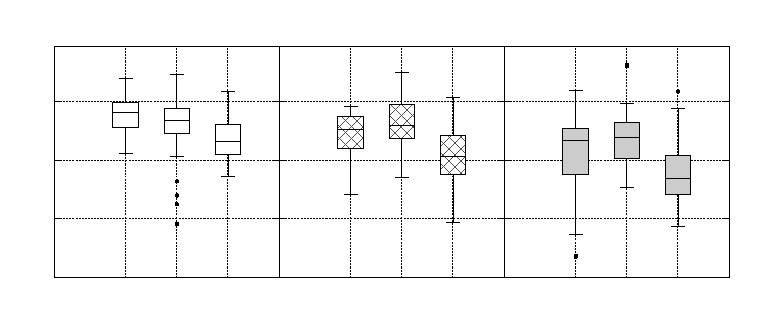
\includegraphics[width={360.00bp},height={144.00bp}]{Fat_latency}}%
    \gplfronttext
  \end{picture}%
\endgroup
}}
    \caption{fat-tree}
    \label{fig:latency:fat}
  \end{subfigure}
   \begin{subfigure}[b]{0.7\columnwidth}
    \resizebox{\textwidth}{!}{\footnotesize{% GNUPLOT: LaTeX picture with Postscript
\begingroup
  \fontfamily{Times-Roman}%
  \selectfont
  \makeatletter
  \providecommand\color[2][]{%
    \GenericError{(gnuplot) \space\space\space\@spaces}{%
      Package color not loaded in conjunction with
      terminal option `colourtext'%
    }{See the gnuplot documentation for explanation.%
    }{Either use 'blacktext' in gnuplot or load the package
      color.sty in LaTeX.}%
    \renewcommand\color[2][]{}%
  }%
  \providecommand\includegraphics[2][]{%
    \GenericError{(gnuplot) \space\space\space\@spaces}{%
      Package graphicx or graphics not loaded%
    }{See the gnuplot documentation for explanation.%
    }{The gnuplot epslatex terminal needs graphicx.sty or graphics.sty.}%
    \renewcommand\includegraphics[2][]{}%
  }%
  \providecommand\rotatebox[2]{#2}%
  \@ifundefined{ifGPcolor}{%
    \newif\ifGPcolor
    \GPcolortrue
  }{}%
  \@ifundefined{ifGPblacktext}{%
    \newif\ifGPblacktext
    \GPblacktexttrue
  }{}%
  % define a \g@addto@macro without @ in the name:
  \let\gplgaddtomacro\g@addto@macro
  % define empty templates for all commands taking text:
  \gdef\gplbacktext{}%
  \gdef\gplfronttext{}%
  \makeatother
  \ifGPblacktext
    % no textcolor at all
    \def\colorrgb#1{}%
    \def\colorgray#1{}%
  \else
    % gray or color?
    \ifGPcolor
      \def\colorrgb#1{\color[rgb]{#1}}%
      \def\colorgray#1{\color[gray]{#1}}%
      \expandafter\def\csname LTw\endcsname{\color{white}}%
      \expandafter\def\csname LTb\endcsname{\color{black}}%
      \expandafter\def\csname LTa\endcsname{\color{black}}%
      \expandafter\def\csname LT0\endcsname{\color[rgb]{1,0,0}}%
      \expandafter\def\csname LT1\endcsname{\color[rgb]{0,1,0}}%
      \expandafter\def\csname LT2\endcsname{\color[rgb]{0,0,1}}%
      \expandafter\def\csname LT3\endcsname{\color[rgb]{1,0,1}}%
      \expandafter\def\csname LT4\endcsname{\color[rgb]{0,1,1}}%
      \expandafter\def\csname LT5\endcsname{\color[rgb]{1,1,0}}%
      \expandafter\def\csname LT6\endcsname{\color[rgb]{0,0,0}}%
      \expandafter\def\csname LT7\endcsname{\color[rgb]{1,0.3,0}}%
      \expandafter\def\csname LT8\endcsname{\color[rgb]{0.5,0.5,0.5}}%
    \else
      % gray
      \def\colorrgb#1{\color{black}}%
      \def\colorgray#1{\color[gray]{#1}}%
      \expandafter\def\csname LTw\endcsname{\color{white}}%
      \expandafter\def\csname LTb\endcsname{\color{black}}%
      \expandafter\def\csname LTa\endcsname{\color{black}}%
      \expandafter\def\csname LT0\endcsname{\color{black}}%
      \expandafter\def\csname LT1\endcsname{\color{black}}%
      \expandafter\def\csname LT2\endcsname{\color{black}}%
      \expandafter\def\csname LT3\endcsname{\color{black}}%
      \expandafter\def\csname LT4\endcsname{\color{black}}%
      \expandafter\def\csname LT5\endcsname{\color{black}}%
      \expandafter\def\csname LT6\endcsname{\color{black}}%
      \expandafter\def\csname LT7\endcsname{\color{black}}%
      \expandafter\def\csname LT8\endcsname{\color{black}}%
    \fi
  \fi
    \setlength{\unitlength}{0.0500bp}%
    \ifx\gptboxheight\undefined%
      \newlength{\gptboxheight}%
      \newlength{\gptboxwidth}%
      \newsavebox{\gptboxtext}%
    \fi%
    \setlength{\fboxrule}{0.5pt}%
    \setlength{\fboxsep}{1pt}%
\begin{picture}(7200.00,2880.00)%
    \gplgaddtomacro\gplbacktext{%
      \csname LTb\endcsname%%
      \put(782,528){\makebox(0,0)[r]{\strut{}$1120$}}%
      \csname LTb\endcsname%%
      \put(782,1089){\makebox(0,0)[r]{\strut{}$1128$}}%
      \csname LTb\endcsname%%
      \put(782,1651){\makebox(0,0)[r]{\strut{}$1136$}}%
      \csname LTb\endcsname%%
      \put(782,2212){\makebox(0,0)[r]{\strut{}$1144$}}%
      \csname LTb\endcsname%%
      \put(1126,242){\rotatebox{25}{\makebox(0,0)[r]{\strut{}SCC}}}%
      \csname LTb\endcsname%%
      \put(1617,242){\rotatebox{25}{\makebox(0,0)[r]{\strut{}CU}}}%
      \csname LTb\endcsname%%
      \put(2107,242){\rotatebox{25}{\makebox(0,0)[r]{\strut{}RWC}}}%
    }%
    \gplgaddtomacro\gplfronttext{%
      \csname LTb\endcsname%%
      \put(137,1482){\rotatebox{-270}{\makebox(0,0){\strut{}Time (ms)}}}%
      \csname LTb\endcsname%%
      \put(1439,2701){\makebox(0,0){\strut{}Nimble}}%
    }%
    \gplgaddtomacro\gplbacktext{%
      \csname LTb\endcsname%%
      \put(2942,528){\makebox(0,0)[r]{\strut{}$2340$}}%
      \csname LTb\endcsname%%
      \put(2942,1089){\makebox(0,0)[r]{\strut{}$2348$}}%
      \csname LTb\endcsname%%
      \put(2942,1651){\makebox(0,0)[r]{\strut{}$2356$}}%
      \csname LTb\endcsname%%
      \put(2942,2212){\makebox(0,0)[r]{\strut{}$2364$}}%
      \csname LTb\endcsname%%
      \put(3286,242){\rotatebox{25}{\makebox(0,0)[r]{\strut{}SCC}}}%
      \csname LTb\endcsname%%
      \put(3777,242){\rotatebox{25}{\makebox(0,0)[r]{\strut{}CU}}}%
      \csname LTb\endcsname%%
      \put(4267,242){\rotatebox{25}{\makebox(0,0)[r]{\strut{}RWC}}}%
    }%
    \gplgaddtomacro\gplfronttext{%
      \csname LTb\endcsname%%
      \put(3599,2701){\makebox(0,0){\strut{}SwingState}}%
    }%
    \gplgaddtomacro\gplbacktext{%
      \csname LTb\endcsname%%
      \put(5102,528){\makebox(0,0)[r]{\strut{}$1520$}}%
      \csname LTb\endcsname%%
      \put(5102,1089){\makebox(0,0)[r]{\strut{}$1532$}}%
      \csname LTb\endcsname%%
      \put(5102,1651){\makebox(0,0)[r]{\strut{}$1544$}}%
      \csname LTb\endcsname%%
      \put(5102,2212){\makebox(0,0)[r]{\strut{}$1556$}}%
      \csname LTb\endcsname%%
      \put(5446,242){\rotatebox{25}{\makebox(0,0)[r]{\strut{}SCC}}}%
      \csname LTb\endcsname%%
      \put(5937,242){\rotatebox{25}{\makebox(0,0)[r]{\strut{}CU}}}%
      \csname LTb\endcsname%%
      \put(6427,242){\rotatebox{25}{\makebox(0,0)[r]{\strut{}RWC}}}%
    }%
    \gplgaddtomacro\gplfronttext{%
      \csname LTb\endcsname%%
      \put(5759,2701){\makebox(0,0){\strut{}OpenNF}}%
    }%
    \gplbacktext
    \put(0,0){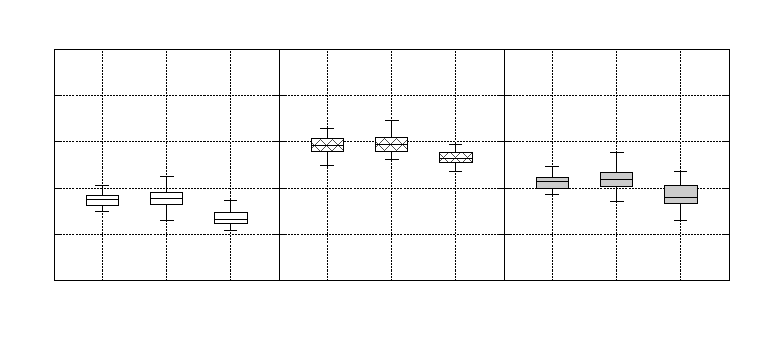
\includegraphics[width={360.00bp},height={144.00bp}]{Forthnet_latency}}%
    \gplfronttext
  \end{picture}%
\endgroup
}}
    \caption{Forthnet}
    \label{fig:latency:forthnet}
  \end{subfigure}
\caption{Times for receiving $10\megabytes$ upon link failure}
\label{fig:latency}
\end{figure}

\chapter{\uppercase{Model Checking}}
\label{chap:modelchecking}
\graphicspath{{./}{./fig/}{./fig/nimble/}}

It is important to prove the correctness of our algorithms. Specifically, we need to verify the suffix causal consistency property for SCC and the waypoint enforcement property for \sysname. In this chapter, we describe how to use model checking to demonstrate the correctness of SCC and \sysname, respectively. Model-checking tools have long been used to check for violations of network properties and automatically find bugs in network applications.  Recent works~\cite{mcopenflow, flowchecker, nice} use model checking to verify network-wide properties for SDN. It is not easy to do so since these methods need to consider the ample space of switch states and the large space of input packets. An SDN switch maintains a flow table that may store a large number of rules and that processes a packet based on the matching rule of the highest priority. Also, the OpenFlow specification allows switches to match packets to rules based on source and destination IP addresses, source MAC addresses, destination MAC addresses, and specific network protocol.  Though prior works try to address these issues use symbolic execution~\cite{symbolic} or simplified switch and packet models, there are additional challenges that prevent existing tools~\cite{mcopenflow, flowchecker, netplumber, hsa, sdnracer, nice, atpg, veriflow} from being directly applied to our algorithms.
 

First, we need to model unknown delays for each switch update to occur since updates are pushed to switches simultaneously (within a single update step for \sysname). This indicates each switch can possibly have an old or new state depending on the delay during the update. Naively, we can use the model checking tool to explore all possibilities for switch states. However, our SCC algorithm guarantees that, once a packet is matched to a forwarding rule in a switch (i.e., reads a switch state), it can be matched in downstream switches only to rules that are equally or more up-to-date (i.e., it cannot read a stale state for downstream switches). Therefore, we explicitly formulate these constraints to model our algorithms. 

Second, our SCC algorithm needs to compare an extra header field $\pktID{}{\tagTmpField}$ of a packet with $\ruleID{}{\epochField}$ when searching for a matching rule on a switch. This field $\pktID{}{\tagTmpField}$ may be updated by any switch depending on the value of $\ruleID{}{\tagTmpField}$. Also, some rules remain unchanged during the previous configurations and thus $\pktID{}{\tagTmpField}$ can be any value from the range of $[1, \epochField]$. To tackle this, our model adds two fields $\ruleID{}{\epochField}$, $\ruleID{}{\tagTmpField}$ for each rule \ruleID{} and a field $\pktID{}{\tagTmpField}$ for each packet \pktID{}. The model checking tool explores all possibilies for $\pktID{}{\tagTmpField}$ as long as the constraints defined for SCC protocol are satisfied.

Third, \sysname can work with any routing-update algorithm that guarantees relaxed waypoint correctness. The update of switches may be executed in multiple steps and in any order. Therefore, the model checking tool cannot focus on only a specific protocol but needs to model diverse protocol behaviors. Our model should also take into account the behavior of the tunnel protocol since \sysname uses tunnels to redistribute packets from old to new positions of network functions. We formulate the definition of relaxed waypoint correctness, simplify the behavior of tunnels and let the model checking tool explore all possible rule-update schedules. Next, we elaborate on how we formulate our models using Z3Py~\cite{z3py}, a Python API for the Z3 solver~\cite{Z3Solver}, and how we use the Z3 solver to verify the desired property. 




%Most of the existing works~\cite{netplumber, hsa, sdnracer, nice, atpg, veriflow} either cannot support the verification of properties we need (suffix causal consistency and waypoint correctness), or is not efficient enough to explore all possible update schedule for violations. Therefore, we use SMT solver to model the network settings and update-schedule algorithms. 

\section{Model checking for SCC}
We subjected SCC to
model checking to verify its enforcement of suffix causal
  consistency, as well as black-hole freedom and bounded looping.
We constructed our model with ten switches in a mesh topology and with
three flows. The maximum length of each routing path was six
  switches.  Each switch was allowed ten rules
($\setSize{\switchID{\switchIdx}{\ruleSet}} \le 10$), which was
  adequate to accommodate the rules deployed by our algorithm for any
  well-formed routing policy for a system of this size.  Deployed
rules satisfied the constraints of \secref{sec:model:net}; e.g., if
$\ruleID{\ruleIdx}, \ruleID{\ruleIdxAlt} \in
\switchID{\switchIdx}{\ruleSet}$ then
$\ruleID{\ruleIdx}{\priorityField} \neq
\ruleID{\ruleIdxAlt}{\priorityField}$ or
$\ruleID{\ruleIdx}{\coverField} \cap \ruleID{\ruleIdxAlt}{\coverField}
= \emptyset$.  The fields of each rule were unspecified and so
explored by the model checker; in particular, each rule could cover
any number of flows.  Each flow was routed from its ingress to its
egress using normal switch behavior (e.g., a switch matches a packet
to the highest priority rule that covers it).  For each initial
  rule $\ruleID{}$, $\ruleID{}{\epochField}$ and
  $\ruleID{}{\tagTmpField}$ were allowed to range over $\{1, 2, 3\}$
  (explored by the model checker). We modeled the effects of one new
  epoch\footnote{This is reasonable since we require that one epoch's
  rule changes are deployed to the network prior to starting the
  next.} ($\epochIdx = 4$) that implemented some different routing
policy (i.e., at least one flow traveled a different
path to its egress) using rules for which \ruleID{}{\epochField} and
\ruleID{}{\tagTmpField} were set according to our algorithm.

Z3 explored all possibilities for each new rule and, so, for the
  new path traversed by each flow, constrained only so that each flow's
  ingress was unchanged.  To model unknown delays for switch updates
to occur, each switch that had not yet applied a new rule to a packet
could apply either an old rule \ruleID{1} or new rule \ruleID{2} to
match the current packet \pktID{}, according to
\pktID{}{\tagTmpField}.  Specifically, if $\pktID{}{\tagTmpField} \le
\ruleID{1}{\epochField}$ and $\pktID{}{\tagTmpField} \le
\ruleID{2}{\epochField}$, either rule could be applied to the packet,
creating two branches. If $\pktID{}{\tagTmpField} >
\ruleID{1}{\epochField}$ and $\pktID{}{\tagTmpField} \le
\ruleID{2}{\epochField}$, then only the new rule $\ruleID{2}$ could be
used to match the packet.

To test black-hole freedom, we set a condition that the trace of
each packet should end with the egress node for the packet. The
bounded looping property was defined to require that any unordered
pair of switches cannot occur in the trace more than twice.
The suffix causal consistency property was modeled to require
  that, once a packet arrives at a switch belonging to its new path
  but not its old path, it stays on the new path.
We let the Z3 solver explore all possible switch configurations to
check for violations of these properties.  In previous, incomplete
versions of our algorithm, this model checking revealed corner cases
that we had failed to consider and that resulted in property
violations; several of these corner cases were used in the examples
given in \secref{sec:algo:controller} to motivate the algorithm
stages.  For the algorithm presented in \secref{sec:algo:controller},
however, after running about $6$ days, the model checker successfully 
terminated and found no violations.



\section{Model Checking for Nimble}
\label{sec:schedule:model_checking}

We subjected our algorithm of \secref{sec:migration} to model checking to verify its enforcement of
waypoint correctness described in \secref{sec:goals:correctness}.
We constructed our model with fifteen switches in a mesh topology and
with three flows.  Each routing path was eight switches and each path
contained three NFs.  We modeled the effects of one new epoch that
implemented a routing policy with NF migration (i.e., each network
function for each flow was moved to a different position) using rules
in the old and new configuration.

The underlying route-update algorithm deployed rule updates on
switches (i.e., deleting unused rules and installing new rules) in at
most $\updateSteps = 15$ steps, with each switch being updated at most
once.  Each switch utilized either old or new rules to process packets
based on the step during which it received those packets. For example,
if \switchID{1} was scheduled to be updated in step \updateID{3},
\switchID{1} used an old rule \ruleID{1} to match \flowID{1} before
\updateID{3} began and a new rule \ruleID{2} after \updateID{3}
completed.  During \updateID{3}, to model unknown delays for switch
updates to occur, either \ruleID{1} or \ruleID{2} was used to match
\flowID{1} nondeterministically. The step at which packets were
received by each switch through the network was non-decreasing.
Moreover, the update schedule generated by the underlying route-update
algorithm ensured relaxed waypoint correctness.  Z3 explored all
possible rule-update schedules constrained by the above conditions to
enforce new routing policy of each flow.  As such, the model checked
was not dependent on any specific route-update protocol, but rather
permitted any route-update strategy as long as it satisfied these
properties.

Our algorithm incorporated NF migration into the rule-update schedule
generated by the underlying route-update algorithm and used tunnels to
redistribute packets from old NF locations to new ones. For
simplicity, the correctness of tunnels was assumed, and tunnels were
not modeled explicitly.  Specifically, when a packet on flow \flowID{}
arrived at \oldSwitchID{\nfIdx} and was matched to rule
\ruleIDIn{\nfIdx}, the packet was delivered to \newSwitchID{\nfIdx},
as if through the tunnel.

To model the delay caused by buffering packets at new NF locations,
the specific step at which \newSwitchID{\nfIdx} forwarded packets
using its new rule should not be earlier than the step at which
\newSwitchID{\nfIdx}{\release{\nfIdx}} is invoked. For example, if a
packet arrived at \oldSwitchID{\nfIdx} for \nfID{\nfIdx} at step
\updateID{3} and then was forwarded through the tunnel to
\newSwitchID{\nfIdx}, \newSwitchID{\nfIdx} could not release packets
until \newSwitchID{\nfIdx}{\release{\nfIdx}} was deployed at step
\updateID{5}. We let the Z3 solver explore all possible delays before
the \newSwitchID{\nfIdx} released packets and check for violations of
waypoint correctness as defined in \secref{sec:goals:correctness}.  In
previous, incorrect versions of our algorithm, this model checking
revealed corner cases that we had failed to consider and that resulted
in property violations.  For the algorithm presented in the previous
sections, however, after running about one day on a 32-core,
2.1\gigahertz computer with 256\gigabytes of memory, the model checker
successfully terminated and found no violations.

\iffalse
\liu{I am not sure if we need this counterexample. It is quite artificial. Just leave here in case you are interested.}
It is hard to determine the time for the controller to deploy \newSwitchID{\nfIdx}{\release{\nfIdx}} on \newSwitchID{\nfIdx} to release packets buffered by \nfID{\nfIdx}.
\mkr{The algorithm in \secref{sec:migration} adds these invocations
  to \updateID{\updateSteps+1}.  Is that wrong?}
In most cases, the controller can send releasing command at step when rule update is scheduled for \newSwitchID{\nfIdx} if the tunnel has been built, since the rule deployment on \newSwitchID{\nfIdx} usually means the downstream switches have been updated and the new forwarding rule on \newSwitchID{\nfIdx} is ready to use. However, our model checking found a counter example shown in \figref{fig:counterexample}. Assume the path of packets was changed from $\switchID{1} \rightarrow \switchID{2} \rightarrow \switchID{3}$ (solid line) to $\switchID{1} \rightarrow \switchID{4} \rightarrow \switchID{5} \rightarrow \switchID{6} \rightarrow \switchID{3}$ (dash line). \nfID{1} was migrated from \switchID{2} to \switchID{4}. The underlying route-update algorithm generated the following rule-update schedule for the path change. The controller updated \switchID{6} and built a tunnel between \switchID{2} and \switchID{4} at step $1$, and then installed forwarding rule on \switchID{4} at step $2$ before updating \switchID{6} at step $3$ and \switchID{5} at step $4$. At last, \switchID{2} was updated to forward packets through the new path so that packets traversed either old or new path. If \switchID{2} received \ruleIDIn{2} at step $2$ and \switchID{4} received \switchID{4}{\release{\nfIdx}} to release packets at step $3$. Packets were dropped on \switchID{5} since it did not have a new rule yet. Therefore, packets can only be released by \newSwitchID{\nfIdx} when \newSwitchID{\nfIdx} starts to receive packets sent from the upstream switch (not through the tunnel).  
\mkr{We should discuss this.  Are you saying that we need to change the
  semantics of the release command?} \liu{This should be an example motivating "update schedule" step in our algorithm.}

\begin{figure}
\centering
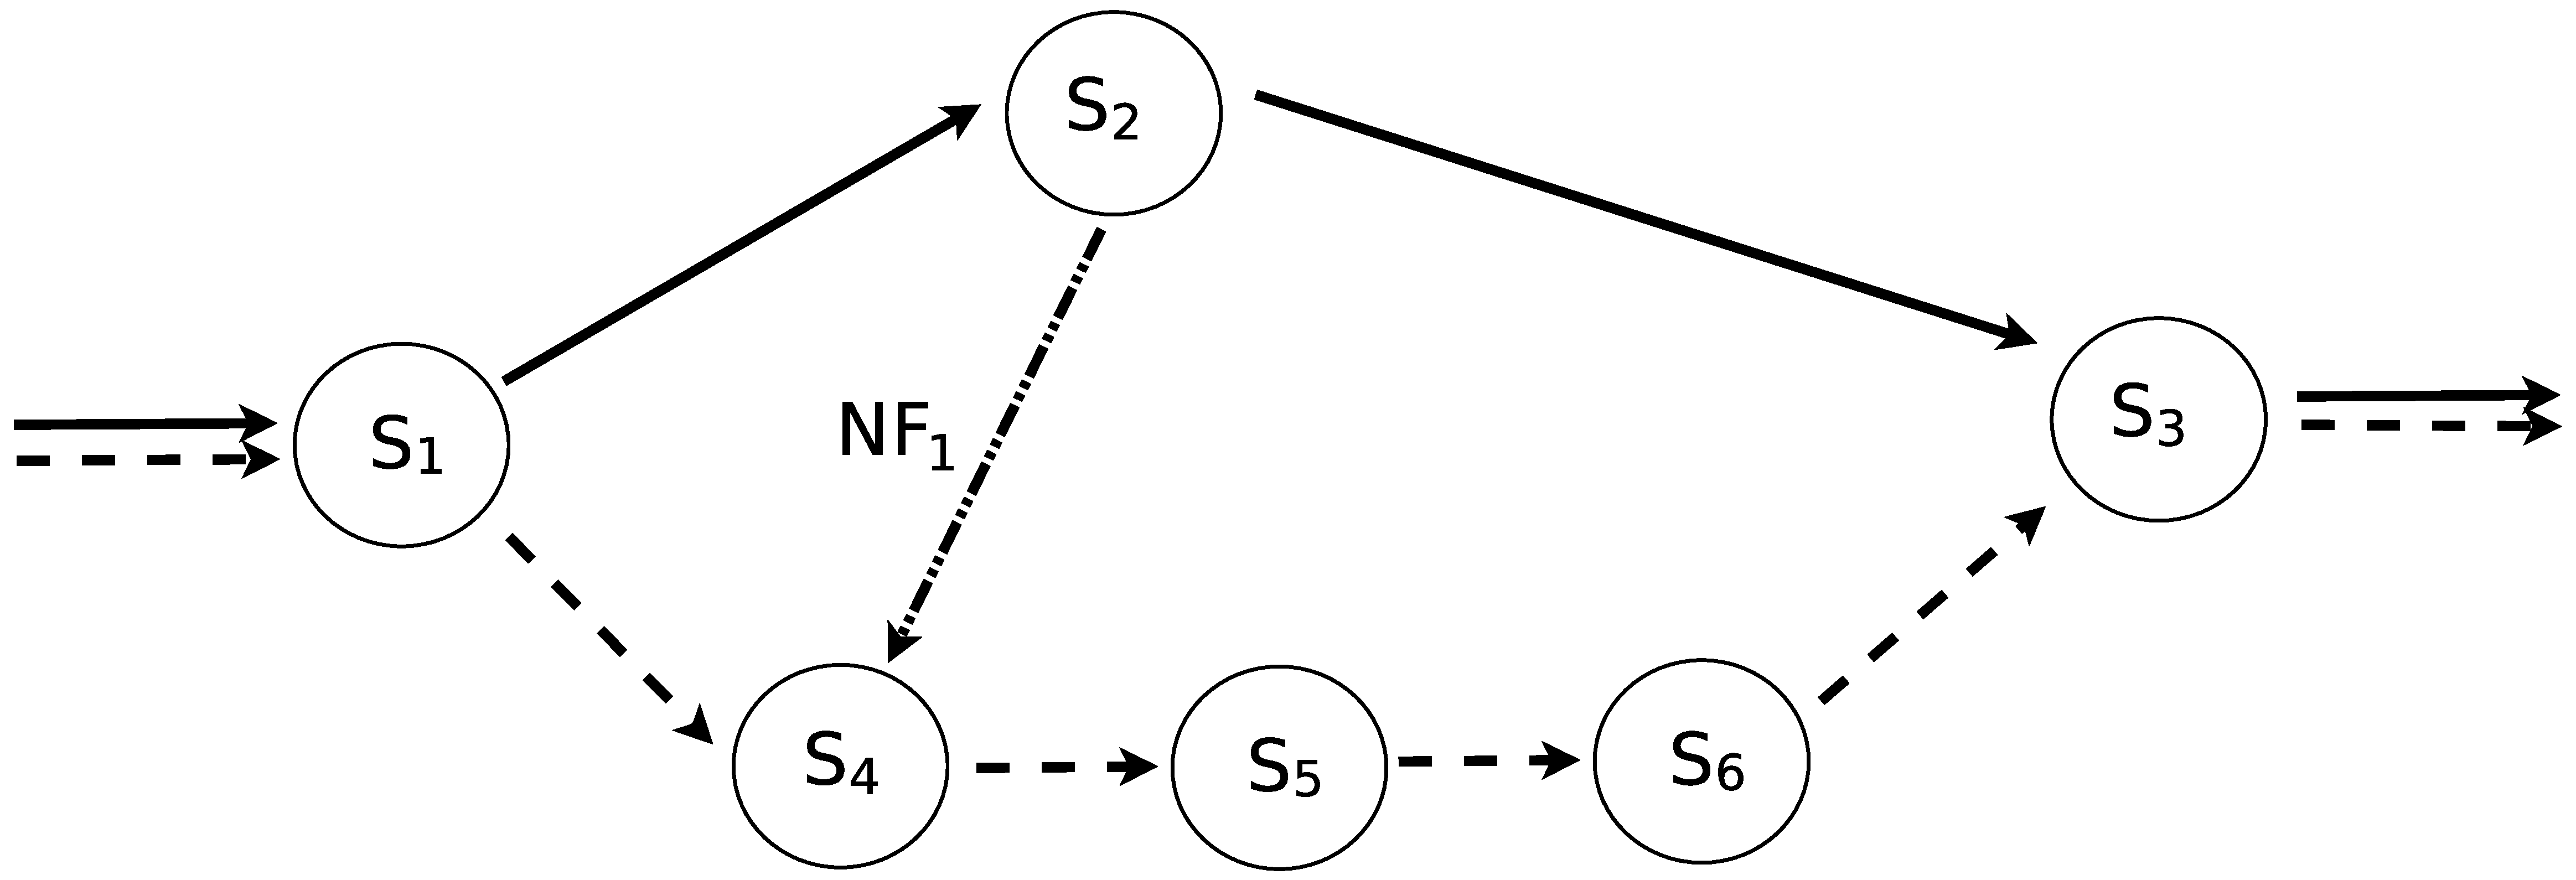
\includegraphics[width=0.45\textwidth]{counterexample.eps}
\vspace{-0.3cm}
\caption{Counterexample for model checking}
\label{fig:counterexample}
\vspace{-0.5cm}
\end{figure}
\fi

\chapter{\uppercase{Conclusion}}

Rapid NF migration and accompanying path changes can be critical for
alleviating problems in a network, and doing so in a way that ensures
that all traffic is processed by its required waypoints is important
to avoid violations of network policy. Realizing this requires both efficient network forwarding-state update and safe NF migration. In this dissertation, we have proposed suffix causal consistency (SCC) as an interpretation of causal consistency for network forwarding-state updates in an SDN network.  SCC ensures that a packet will be matched only to rules at least as recent as
those to which it has been matched previously, thus ensuring that a
packet will exit the network on a suffix of the most recent path's
rules to which it was matched.  Our algorithm implements this property
without updating switches unnecessarily.  We showed that SCC
implements bounded looping and black-hole freedom during updates and
formally verified that our algorithm achieves SCC as well as these
additional properties.  Through empirical tests with implementations
in P4 and Open vSwitch, and using real traffic traces from Facebook,
we showed that our algorithm supports faster rule deployment than CU,
TSU and COCONUT, leading to fewer dropped packets during updates.  SCC also requires the retention of fewer additional rules during the update, and its rule generation scales across a wide range of topologies.


To coordinate NF migration with the routing policy update, we have
presented an algorithm that accelerates the deployment of these
changes in SDN networks over current best solutions.  Our design
accomplishes this through a careful interleaving of NF migrations with
path changes, and ensures the correctness of traffic processing provided
that the route-update protocol on which we build ensures a property
that we call \textit{relaxed waypoint correctness}.  We provided a
route-update protocol designed to achieve this property, without
enforcing other properties typically associated with consistent-update
protocols.  We showed the sufficiency of this property through model
checking, and then demonstrated the performance improvements achieved by our algorithm in empirical comparisons to state-of-the-art.

We believe our work paves the way for future research in SDN and network function migration. For example, is it feasible to balance the workload of each network function by choosing where NFs should be migrated to and which path traffic should be rerouted through?  Is it possible to design a one big switch framework that can automatically and consistently manage state for programmable switches? We leave these open issues for future work. 


%%%%%%%%%%%%%%%%%%%%%%%%%%%%%%%%
%% BIBLIOGRAPHY AND OTHER LISTS
%%%%%%%%%%%%%%%%%%%%%%%%%%%%%%%%
\backmatter

% Bibliography
\bibliography{dissertation}
%\addtocontentsline{toc}{\protect\vspace*{\baselineskip}}

% Add bibliography to contents page
%\addcontentsline{toc}{chapter}{Bibliography} %'Bibliography' into toc



\end{document}
